%%%%%%%%%%%%%%%%%%%%%%%%%%%%%%%%%%%%%%%%%%%%%%%%%%%%%%%%%%%%%%%%%%%%%%%%
\clearpage
\section{Cylindrical objects}
\label{sect:CylindricalObjects}

\subsection{Disc}
\label{sect:Disc}
\hspace{1pt} \\

\begin{figure}[htb]
\begin{center}
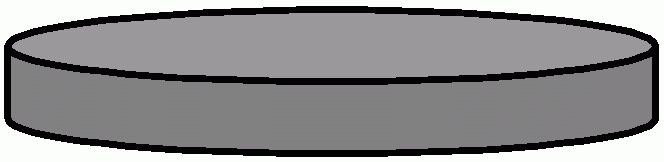
\includegraphics[width=0.5\textwidth]{../images/form_factor/cylindrical_obj/disc.png}
\end{center}
\caption{} \label{disc}
\end{figure}
\begin{align}
I_\text{Disc}(q,R)=\pi^2R^4\Delta\eta^2\frac{2}{(qR)^2}
\left(1-\frac{1}{qR}\text{J}_1(2qR)\right)
\end{align}
with $\DS \lim_{q=0}I_\text{Disc}(q,R) = \pi^2R^4\Delta\eta^2$

\vspace{5mm}

\uline{Input Parameters for model \texttt{Disc}:}
\begin{description}
\item[\texttt{R}] radius of disc $R$
\item[\texttt{eta}] scattering contrast $\Delta\eta$
\end{description}

\noindent\uline{Note:}
\begin{itemize}
\item none
\end{itemize}

\begin{figure}[htb]
\begin{center}
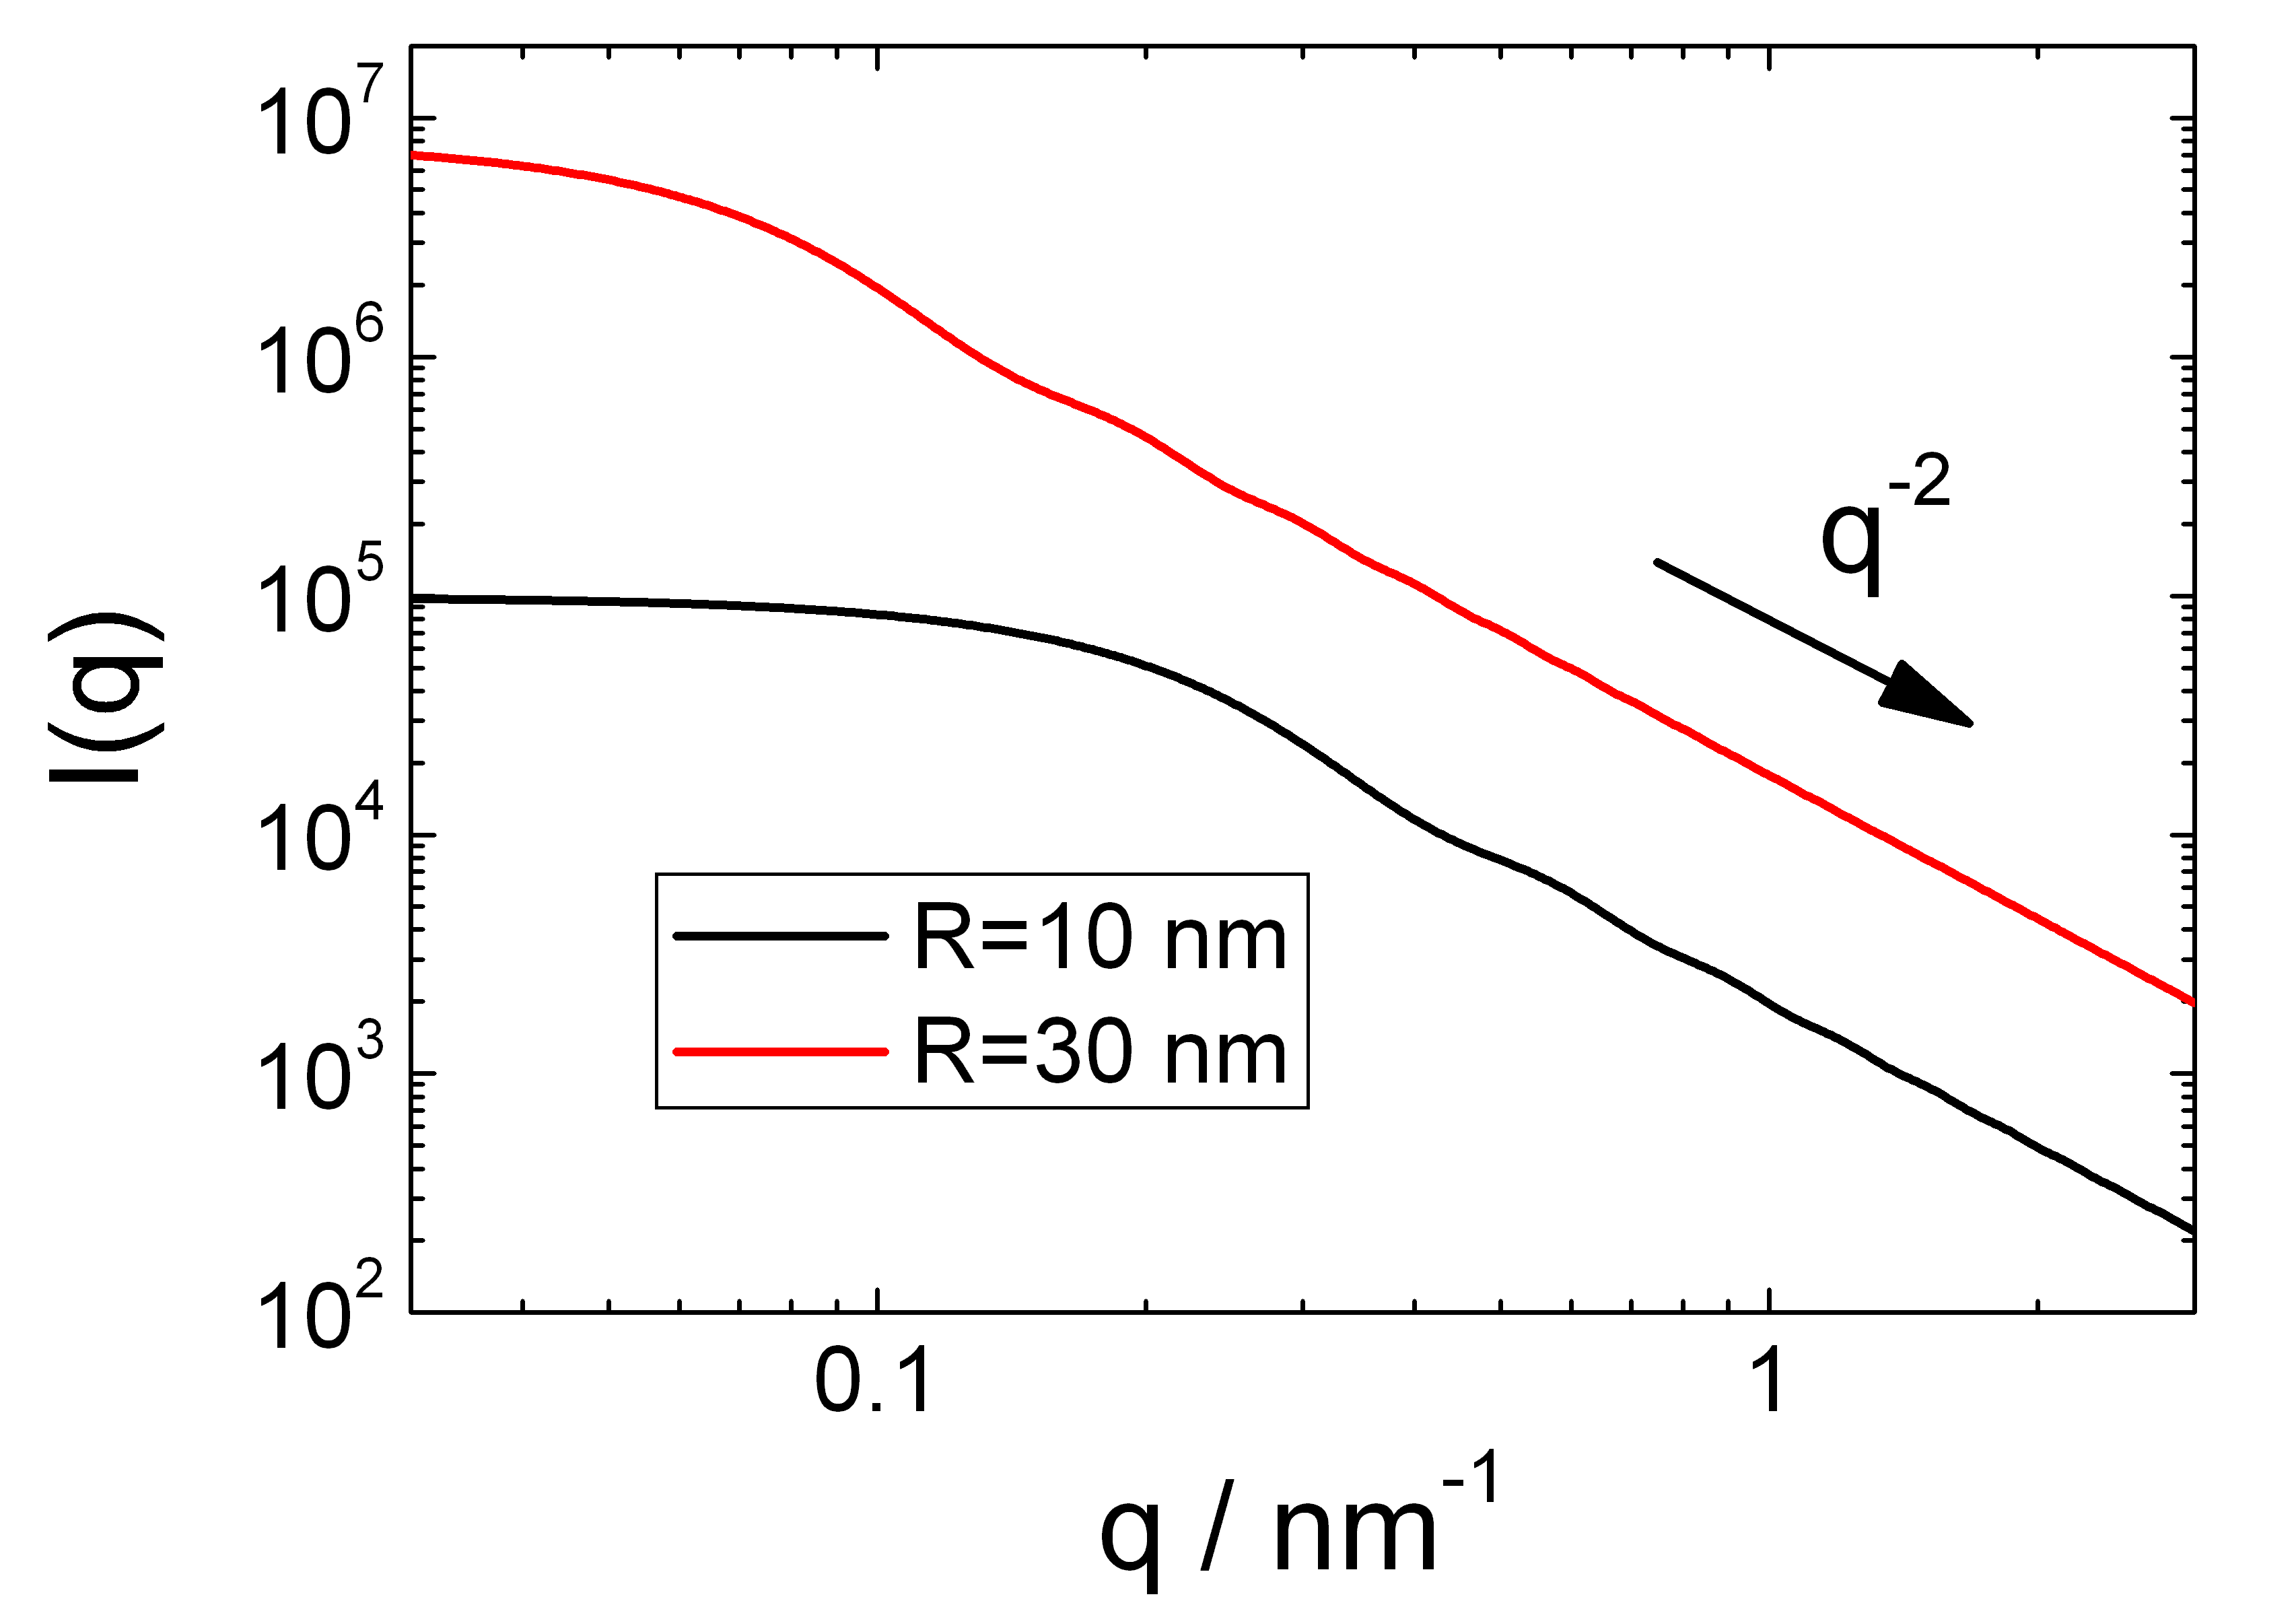
\includegraphics[width=0.668\textwidth]{../images/form_factor/cylindrical_obj/DiscIQ.png}
\end{center}
\caption{Scattering intensity of a disc with radii $R=10$ nm and $R=30$ nm.
The scattering length density contrast is set to 1.}
\label{fig:I_disc}
\end{figure}

%%%%%%%%%%%%%%%%%%%%%%%%%%%%%%%%%%%%%%%%%%%%%%%%%%%%%%%%%%%%%%%%%

\newpage
\subsection{Rod}
\label{sect:Rod}
~\\

\begin{figure}[htb]
\begin{center}
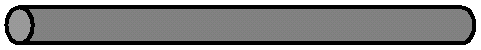
\includegraphics[width=0.5\textwidth]{../images/form_factor/cylindrical_obj/rod.png}
\end{center}
\caption{} \label{rod}
\end{figure}
\begin{align}
I_\text{Rod}(q,L) = \Delta\eta^2L^2\left(\frac{2}{qL}\text{Si}(qL)
                                         - \left(\frac{\sin(qL/2)}{qL/2}\right)^2
                                   \right)
\end{align}
with $\DS \text{Si}(x)=\int_0^x\!\frac{\sin t}{t}\,\,dt$ and $\DS
\lim_{q=0} I_\text{Rod}(q,L) = \Delta\eta^2L^2$

\vspace{5mm}

\uline{Input Parameters for model \texttt{Rod}:}
\begin{description}
\item[\texttt{L}] length of rod $L$
\item[\texttt{eta}] scattering contrast $\Delta\eta$
\end{description}

\uline{Note:}
\begin{itemize}
\item none
\end{itemize}

\begin{figure}[htb]
\begin{center}
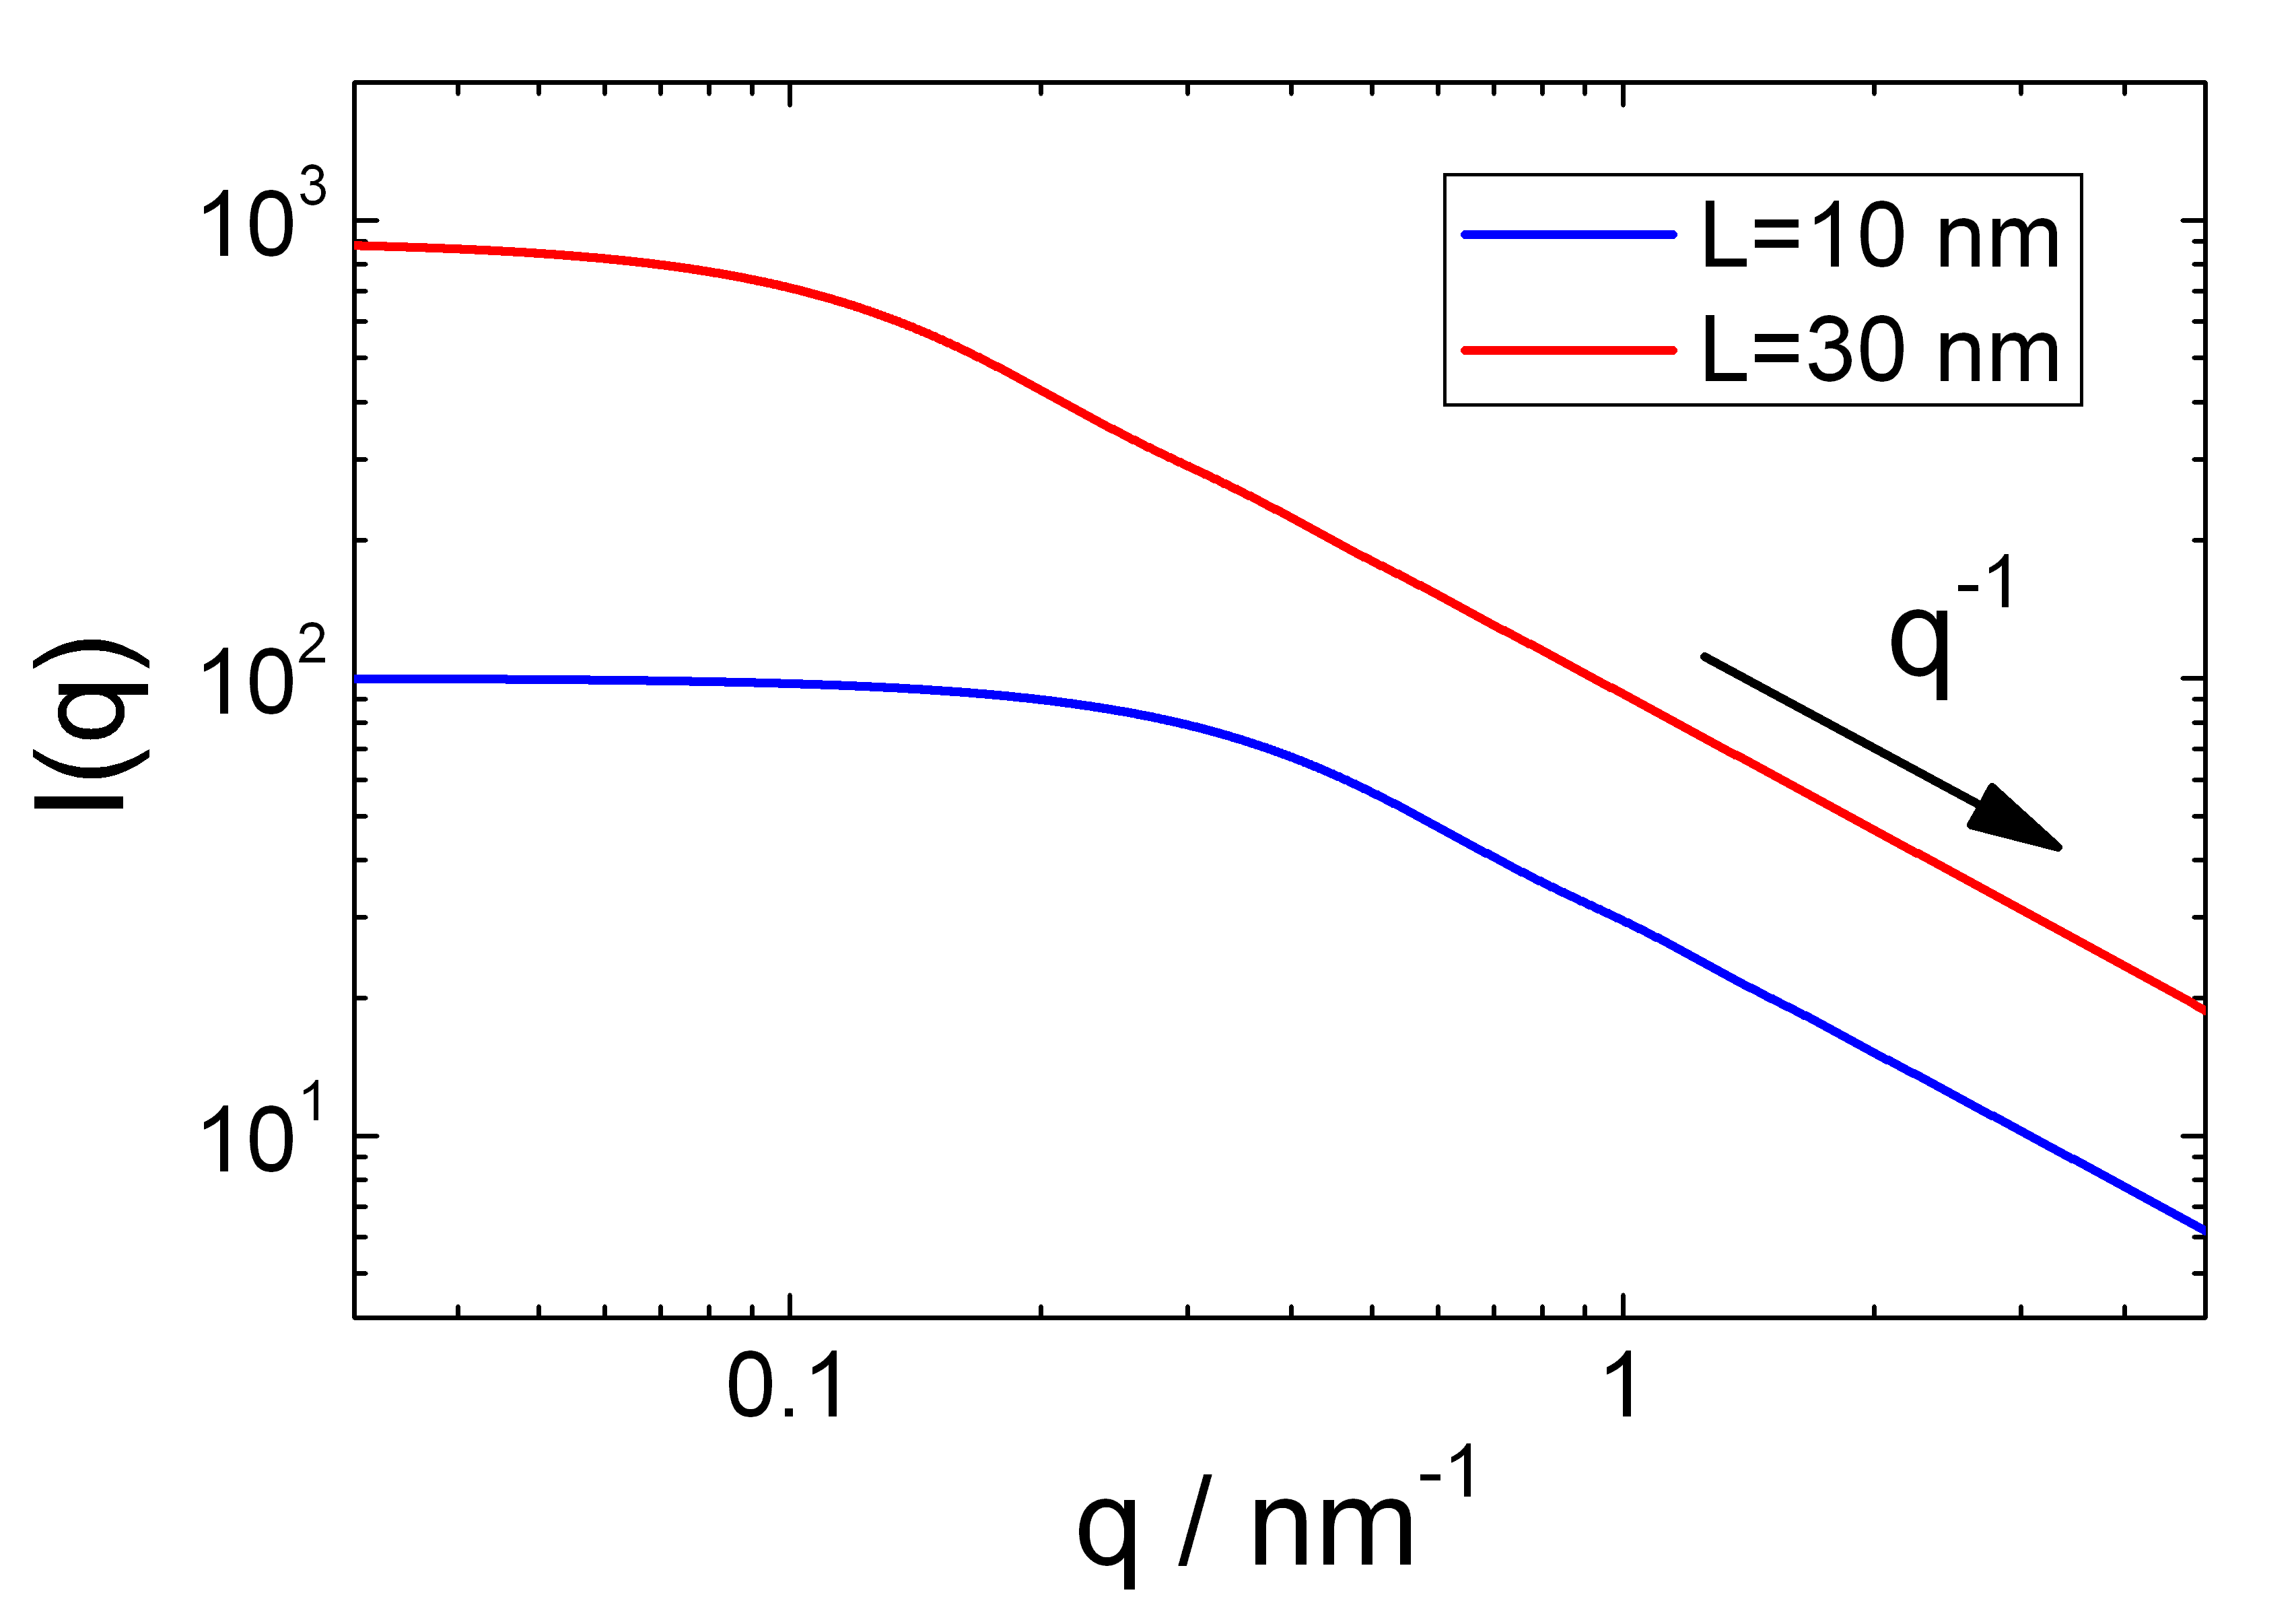
\includegraphics[width=0.668\textwidth]{../images/form_factor/cylindrical_obj/RodIQ.png}
\end{center}
\caption{Scattering intensity of a rod of length $L=10$ nm and $L=30$ nm.
The scattering length density contrast is set to 1.}
\label{fig:I_rod}
\end{figure}
%%%%%%%%%%%%%%%%%%%%%%%%%%%%%%%%%%%%%%%%%%%%%%%%%%%%%%%%%%%%%%%%%%%%%%

\clearpage
\subsection{Porod's approximation for a long cylinder} \cite{Porod1948}
\label{sect:LongCylinder}
~\\

\begin{figure}[htb]
\begin{center}
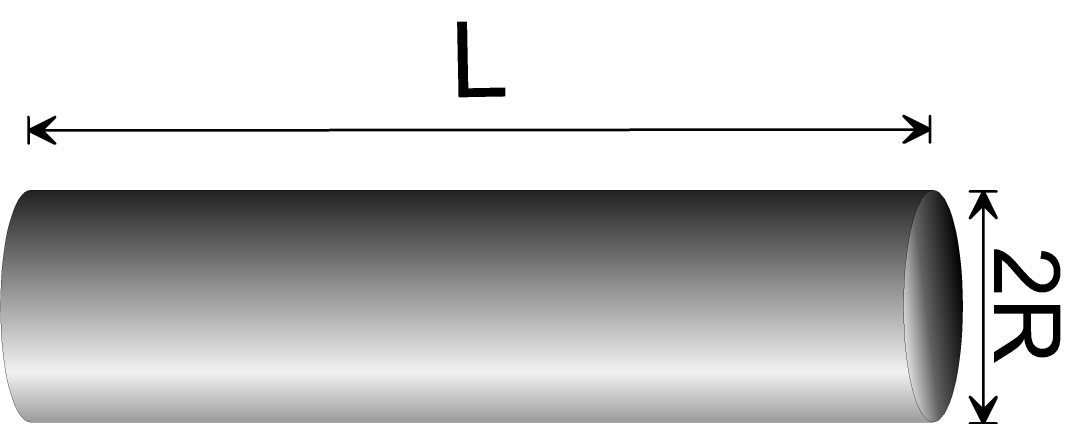
\includegraphics[width=0.8\textwidth]{../images/form_factor/cylindrical_obj/long_cylinder.png}
\end{center}
\caption{} \label{longcylinder}
\end{figure}

\begin{align}
\text{Si}_\frac{\pi}{2}(x) &= \left( \mathrm{Si}(x)+\frac{\cos x}{x}+\frac{\sin x}{x^2} \right)
\quad \xrightarrow{x \rightarrow\infty} \quad \frac{\pi}{2} \\
\Lambda_1(x) &= \frac{2}{x} \mathrm{J}_1(x) \\
\Lambda_2(x) &= \frac{8}{x^2} \mathrm{J}_2(x) \\
\omega(x) &= \frac{8}{x^2} \left(3 \mathrm{J}_2(x) +\mathrm{J}_0(x)-1\right) \\
%\Phi_\text{disc}(x) &= \frac{2}{x^2}
%\left[1-\Lambda_1(x)\right] \\
\Phi_\text{long}(q,R,L) &= \left(\Delta\eta\pi
R^2L\right)^2 \frac{2}{QL}  \label{eq:LongCylinder}\\
& \quad \times \left\{\text{Si}_\frac{\pi}{2}(QL)\Lambda_1^2(QR)
%-\frac{2\Lambda_2(2QR)-\Phi_\text{disc}(2QR)}{QL}
-\frac{\omega(2QR)}{QL}
-\frac{\sin(QL)}{(QL)^2}\right\}\nonumber
\end{align}
$\mathrm{J}_n(x)$ are the regular cylindrical Bessel function of order $n$.

\vspace{5mm}

\uline{Input Parameters for model \texttt{LongCylinder}:}
\begin{description}
\item[\texttt{R}] radius of cylinder $R$
\item[\texttt{L}] length of cylinder $L$
\item[\texttt{eta}] scattering contrast $\Delta\eta$
\end{description}

\uline{Note:}
\begin{itemize}
\item The approximation is valid for $L>2R$
\end{itemize}

\begin{figure}[htb]
\begin{center}
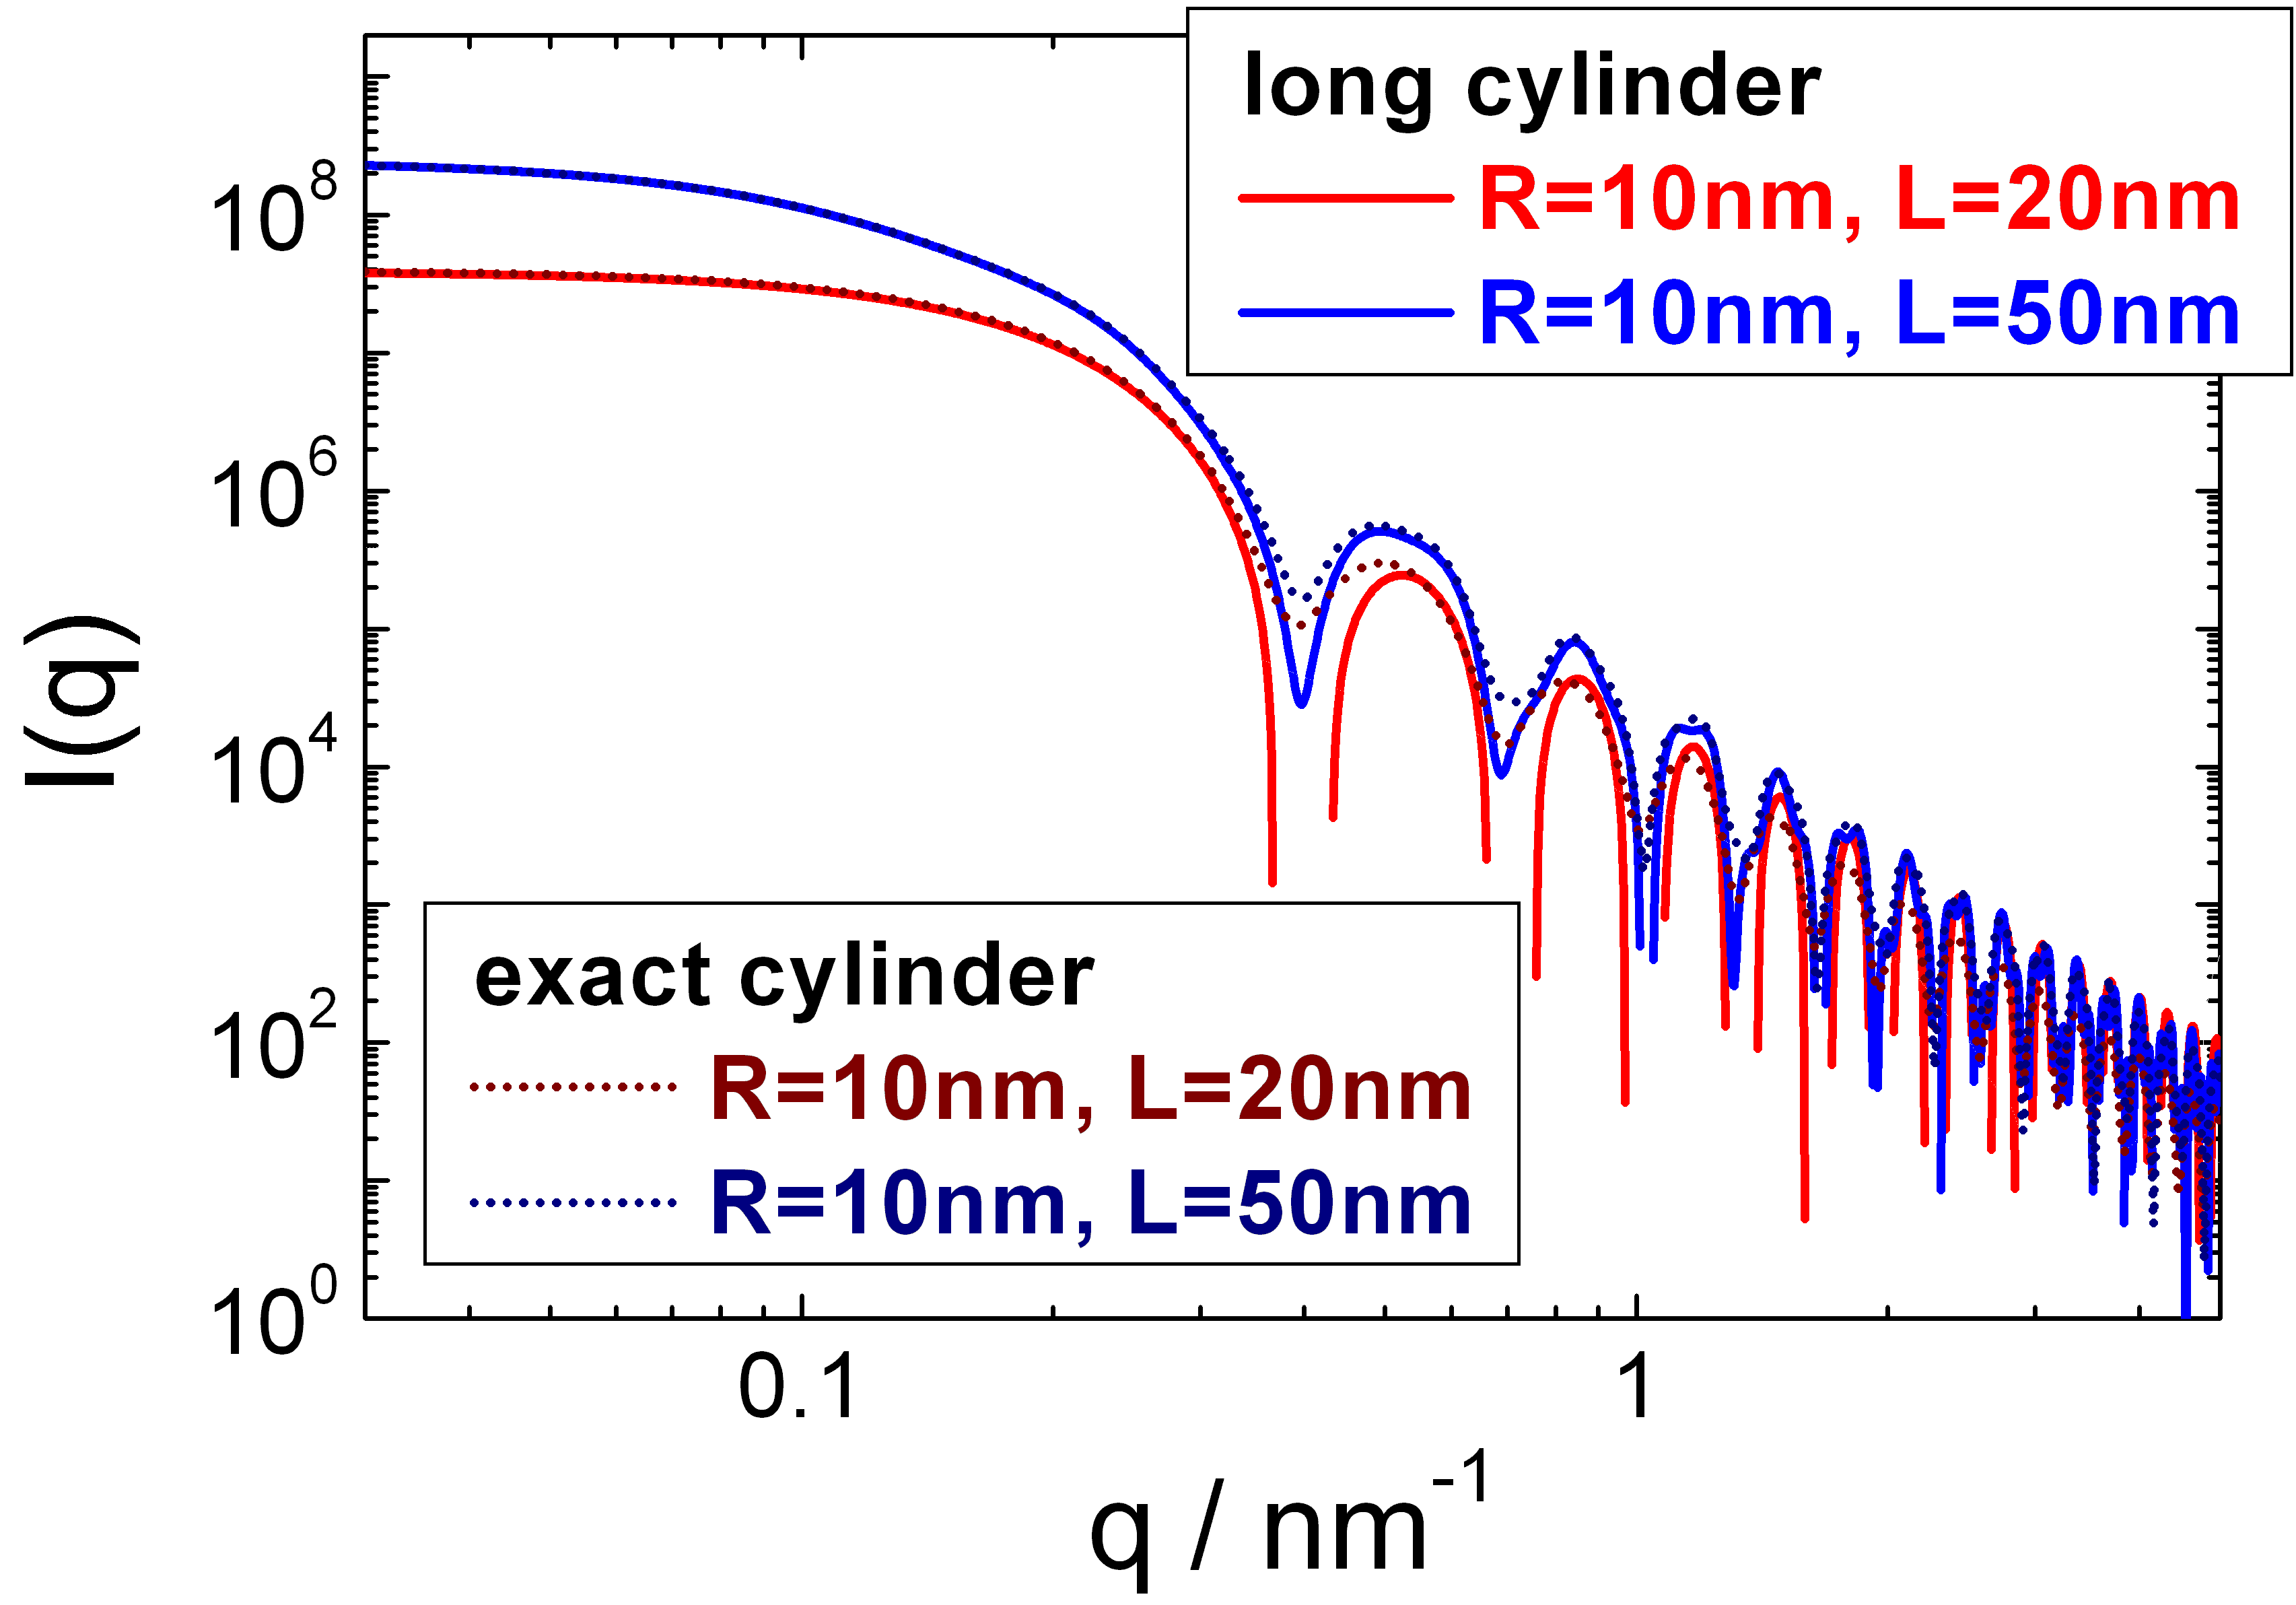
\includegraphics[width=0.668\textwidth]{../images/form_factor/cylindrical_obj/LongCylinder.png}
\end{center}
\caption{Scattering intensity of a cylinder with radius $R=10$ nm and lengths of $L=20$ nm
and $L=50$ nm. Next to Porod's approximation for long cylinders also
the exact integral solution is shown for comparison.
The scattering length density contrast is set to 1.}
\label{fig:LongCylinder}
\end{figure}

%%%%%%%%%%%%%%%%%%%%%%%%%%%%%%%%%%%%%%%%%%%%%%%%%%%%%%%%%%%%%%%%%%%%%%%%%%%%%%%%

\clearpage
\subsection{Porod's approximation for a flat cylinder} \cite{Porod1948}
\label{sect:flatCylinder}
~\\

\begin{figure}[htb]
\begin{center}
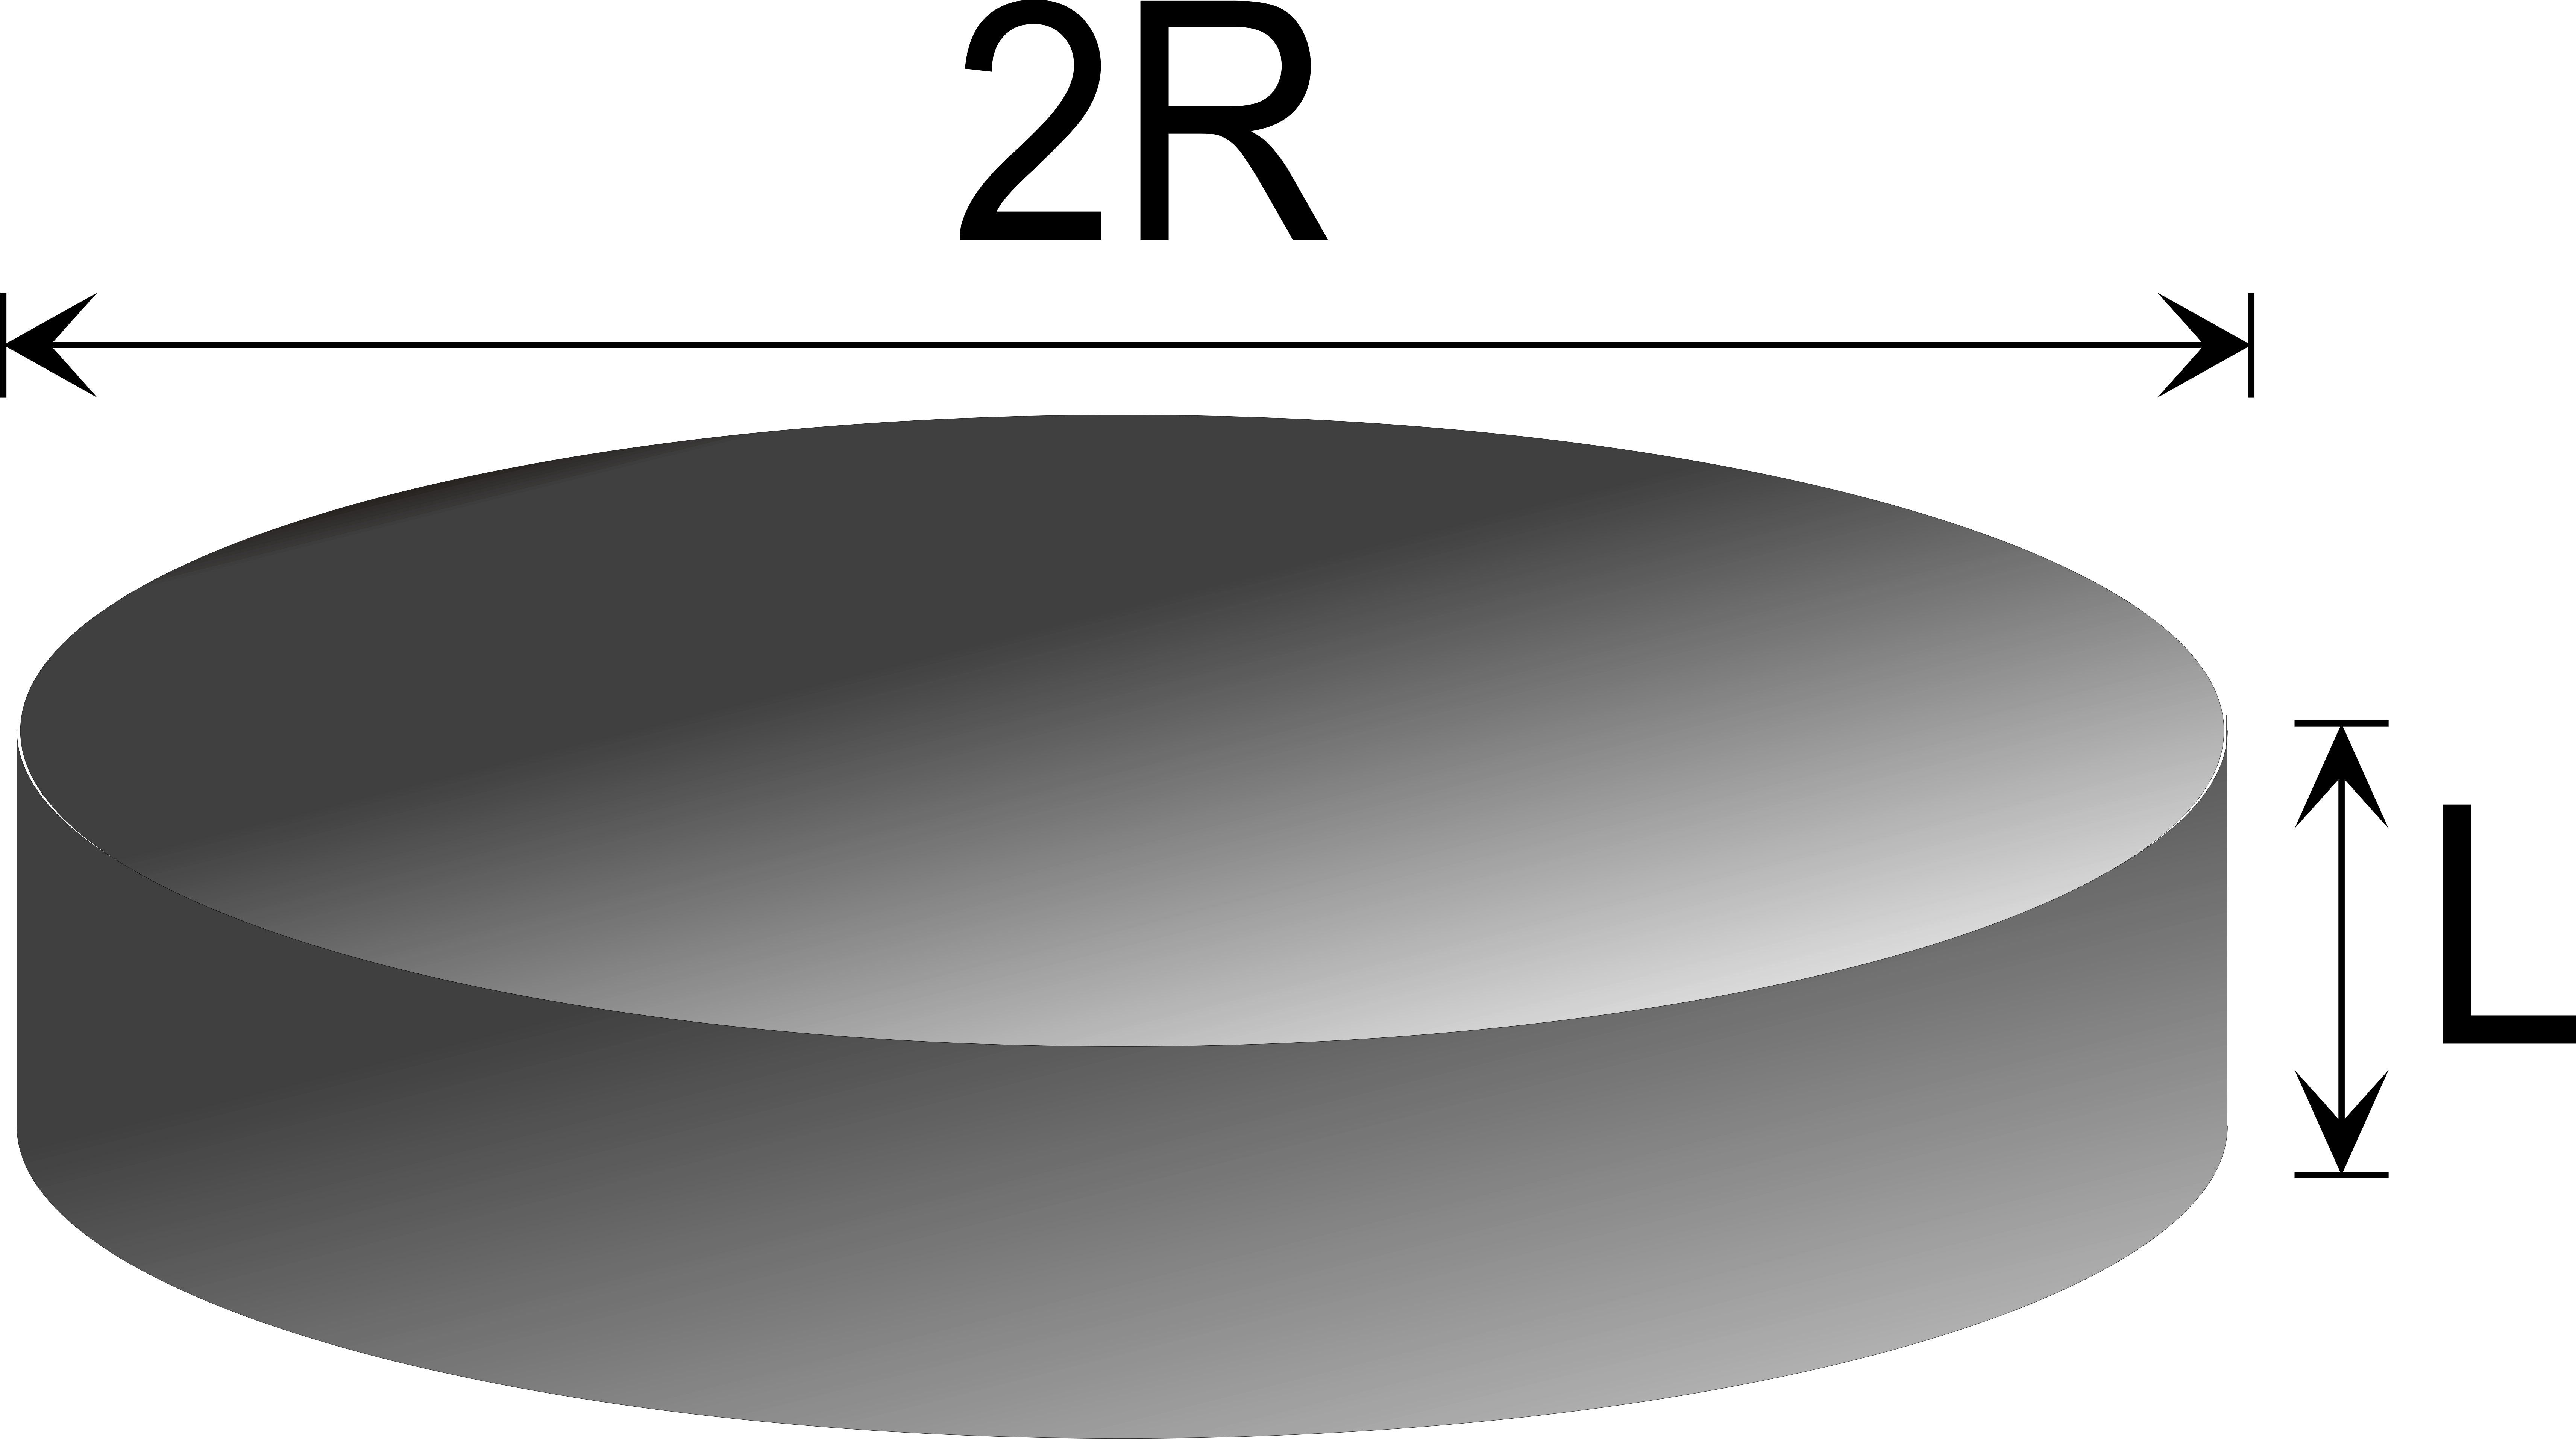
\includegraphics[width=0.7\textwidth]{../images/form_factor/cylindrical_obj/flat_cylinder.png}
\end{center}
\caption{} \label{flatcylinder}
\end{figure}

\begin{align}
\Lambda_1(x) &= \frac{2}{x} J_1(x) \\
I_1(x) &= \int\limits_0^x \Lambda_1(x') dx' = \\
& \quad 2x \mathrm{J}_0(x)-2\mathrm{J}_1(x)-\pi x \left[J_0(x)\mathrm{H}_1(x)-\mathrm{J}_1(x)\mathrm{H}_0(x)\right] \nonumber \\
I_0(x) &= \frac{I_1(x)+x\Lambda_1(x)}{2}\\
\Omega(x) &= \frac{2}{x} \left[ I_0(x)-2\mathrm{J}_1(x)\right]\\
\chi(x) &= \left( \frac{\sin(x/2)}{x/2}\right)^2\\
\Phi_\text{flat}(q,R,L) &= \left(\Delta\eta\pi R^2L\right)^2 \frac{8}{(2qR)^2}  \label{eq:FlatCylinder}\\
& \quad \times \left\{ \chi(qL) +
\frac{I_1(2QR)\;\Omega(qL)}{2qR}-\Lambda_1(2qR)\right\}\nonumber
\end{align}
$\mathrm{H}_\alpha(x)$ is the Struve function of order $\alpha$ and $\mathrm{J}_n(x)$ are the regular cylindrical Bessel function of order $n$.

\vspace{5mm}

\uline{Input Parameters for model \texttt{FlatCylinder}:}
\begin{description}
\item[\texttt{R}] radius of cylinder $R$
\item[\texttt{L}] length of cylinder $L$
\item[\texttt{eta}] scattering contrast $\Delta\eta$
\end{description}

\uline{Note:}
\begin{itemize}
\item The approximation is valid for $L<2R$
\end{itemize}

\begin{figure}[htb]
\begin{center}
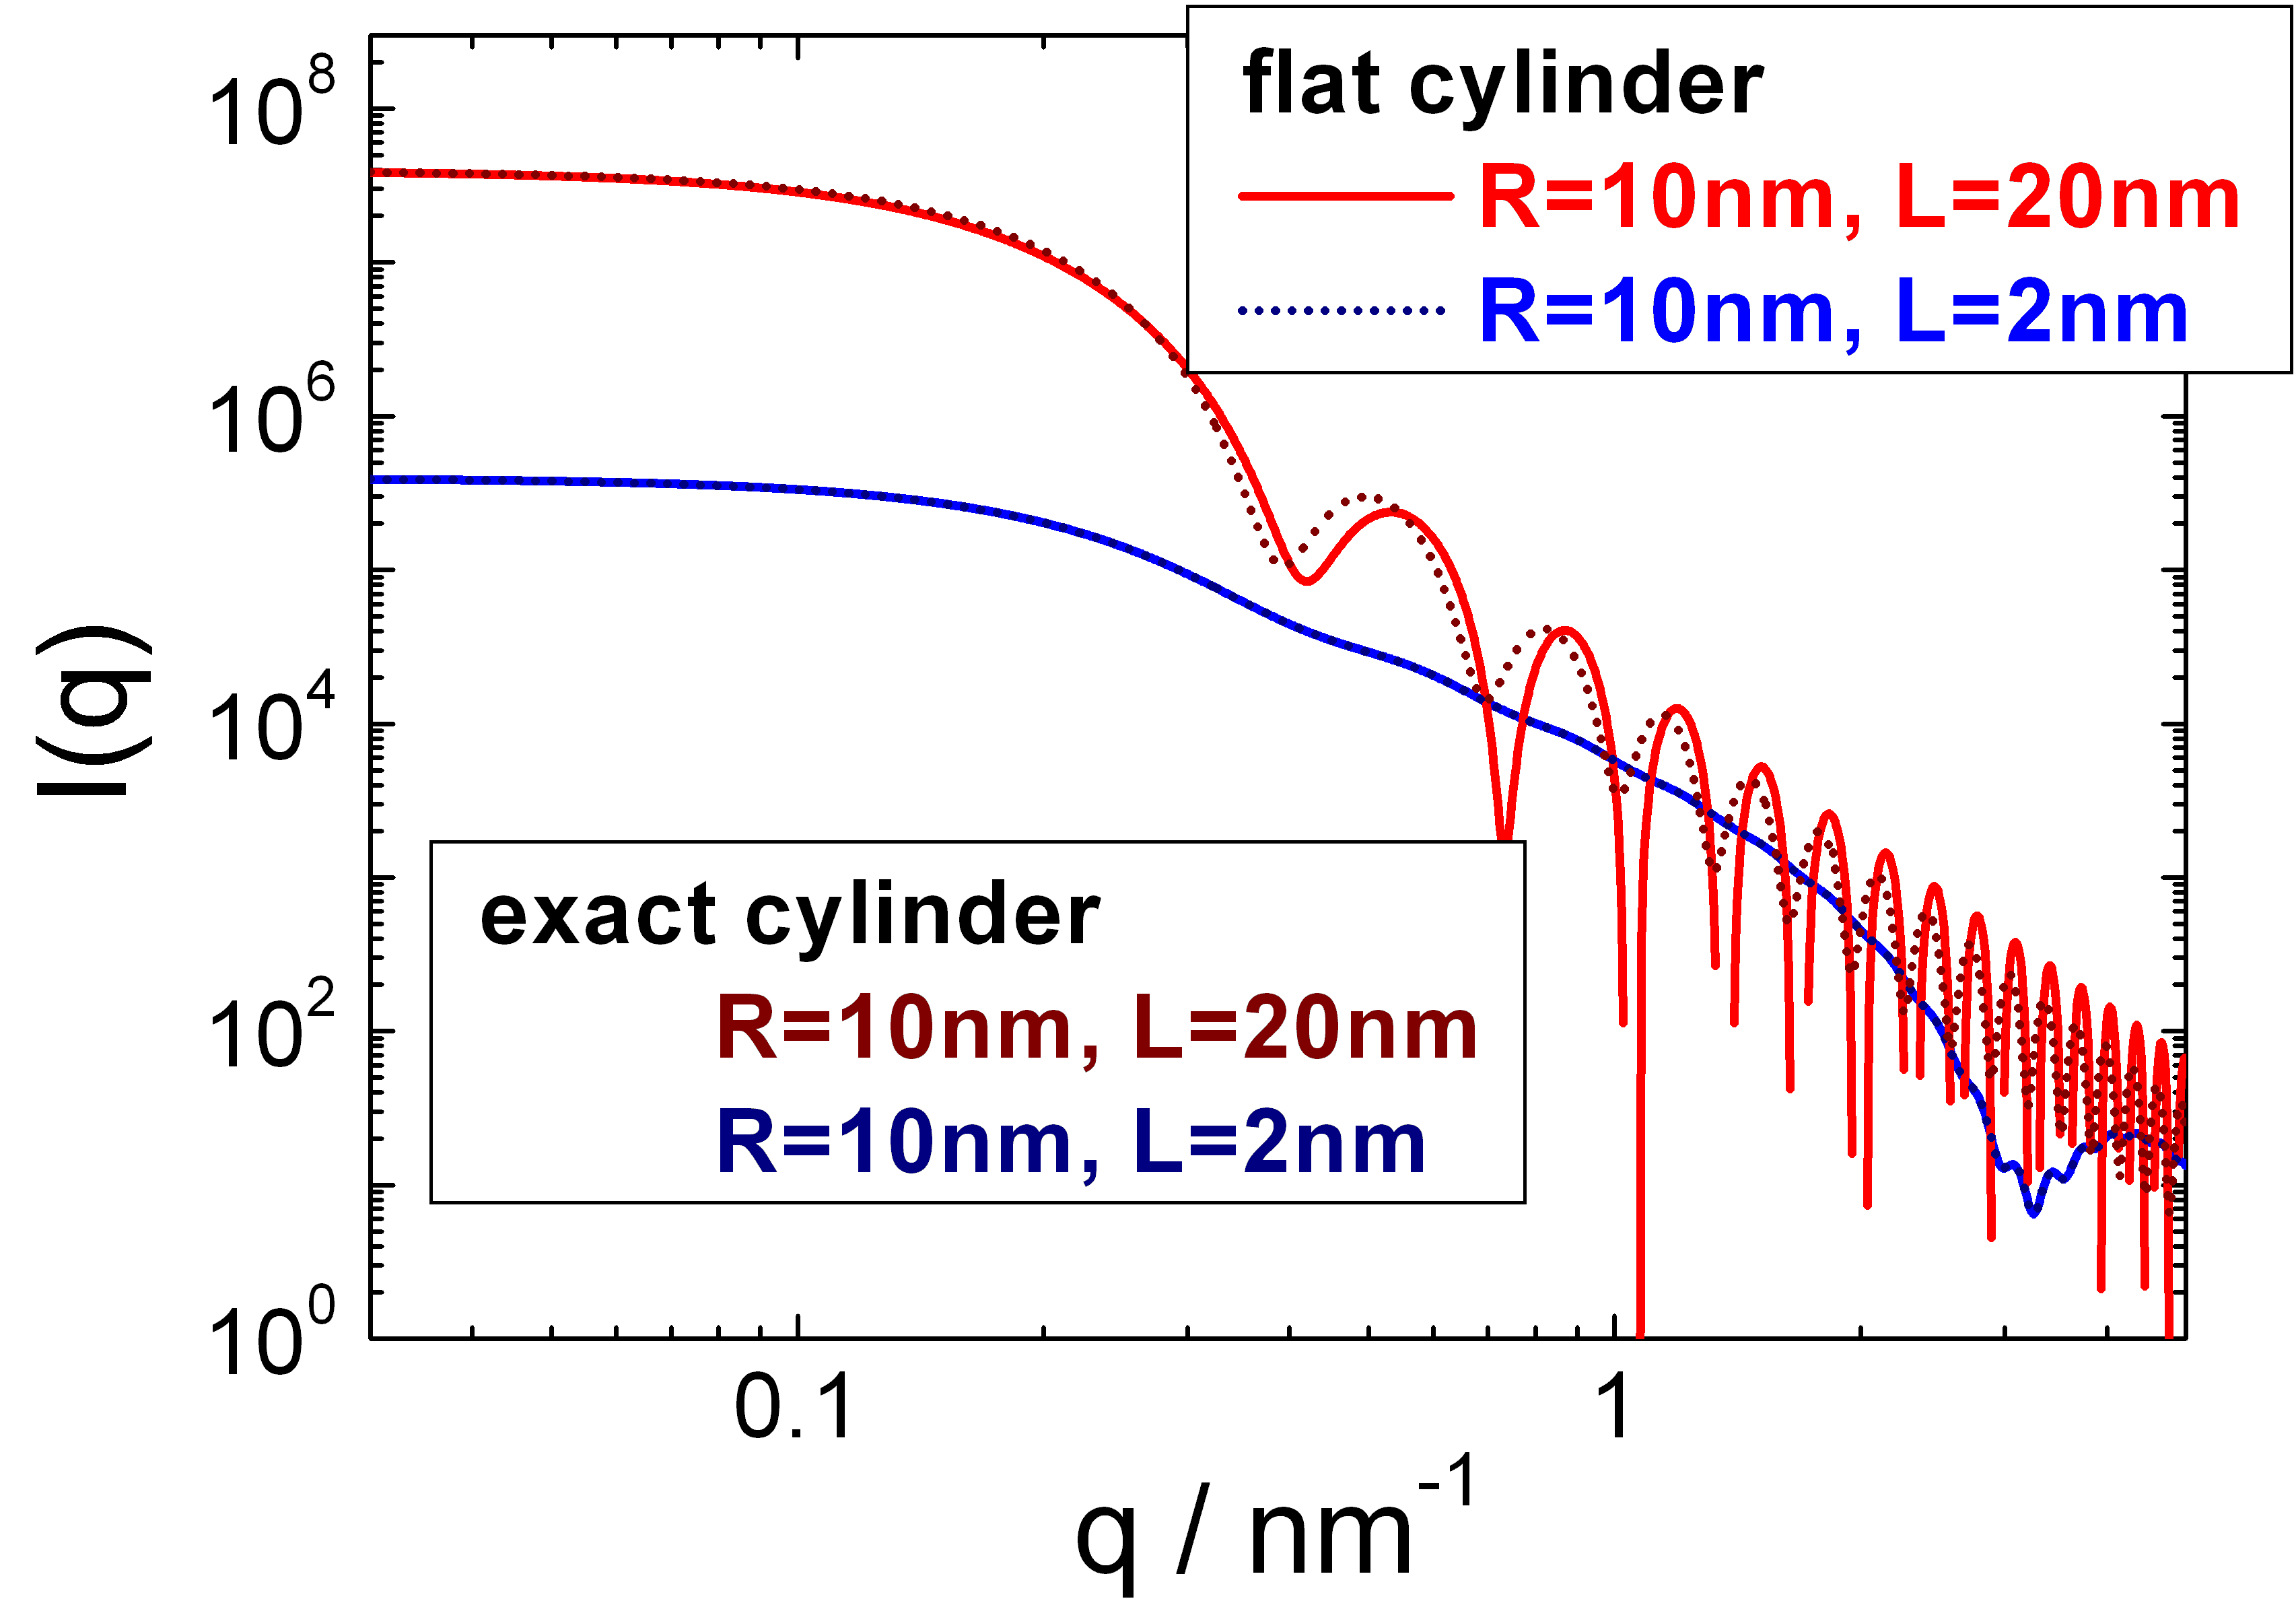
\includegraphics[width=0.668\textwidth]{../images/form_factor/cylindrical_obj/FlatCylinder.png}
\end{center}
\caption{Scattering intensity of a cylinder with radius $R=10$ nm and lengths of $L=2$ nm
and $L=20$ nm. Next to Porod's approximation for flat cylinders also
the exact integral solution is shown for comparison.
The scattering length density contrast is set to 1.}
\label{fig:FlatCylinder}
\end{figure}

\clearpage

\subsection{Porod's approximations for cylinder} \cite{Porod1948}
\label{sect:PorodCylinder}
~\\
\begin{figure}[htb]
\begin{center}
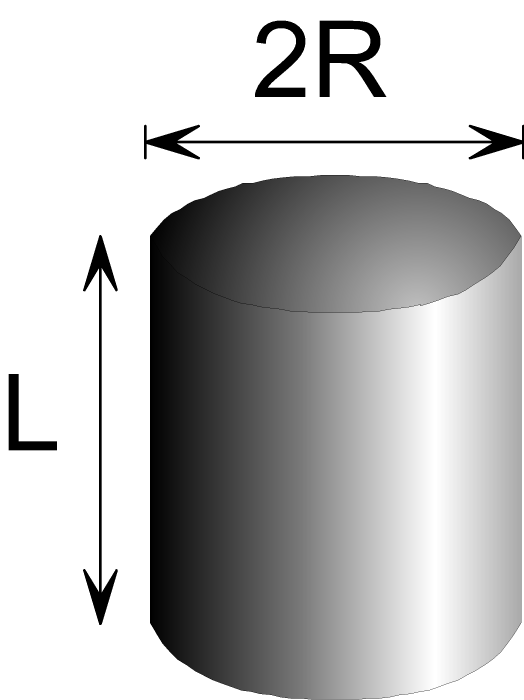
\includegraphics[width=0.288\textwidth]{../images/form_factor/cylindrical_obj/cylinder.png}
\end{center}
\caption{} \label{PorodCylinder}
\end{figure}

This form factor combines the two solutions of Porod for a long $\Phi_\text{long}(q,R,L)$
(\ref{eq:LongCylinder}) and a flat $\Phi_\text{flat}(q,R,L)$ (\ref{eq:FlatCylinder}) cylinder
by a linear combination of both. A simple linear transition at $L=2R$ is assumed.
\begin{align}
\Phi_\text{Porod}(q,R,L) &= p\left(\frac{2R}{L}\right)\Phi_\text{flat}(q,R,L) + \left(1-p\left(\frac{2R}{L}\right)\right)\Phi_\text{long}(q,R,L) \\
p(x) &=
\begin{cases}
    1 & \mbox{for } x > \frac54 \\
    2\left(x-\frac34\right) & \mbox{for }\frac34 \leq x \leq \frac54 \\
    0 & \mbox{for } x < \frac34
\end{cases}
\end{align}

\vspace{5mm}

\uline{Input Parameters for model \texttt{PorodCylinder}:}
\begin{description}
\item[\texttt{R}] radius of cylinder $R$
\item[\texttt{L}] length of cylinder $L$
\item[\texttt{eta}] scattering contrast $\Delta\eta$
\end{description}

\uline{Note:}
\begin{itemize}
\item less good approximation  for $L \sim 2R$
\end{itemize}

\begin{figure}[htb]
\begin{center}
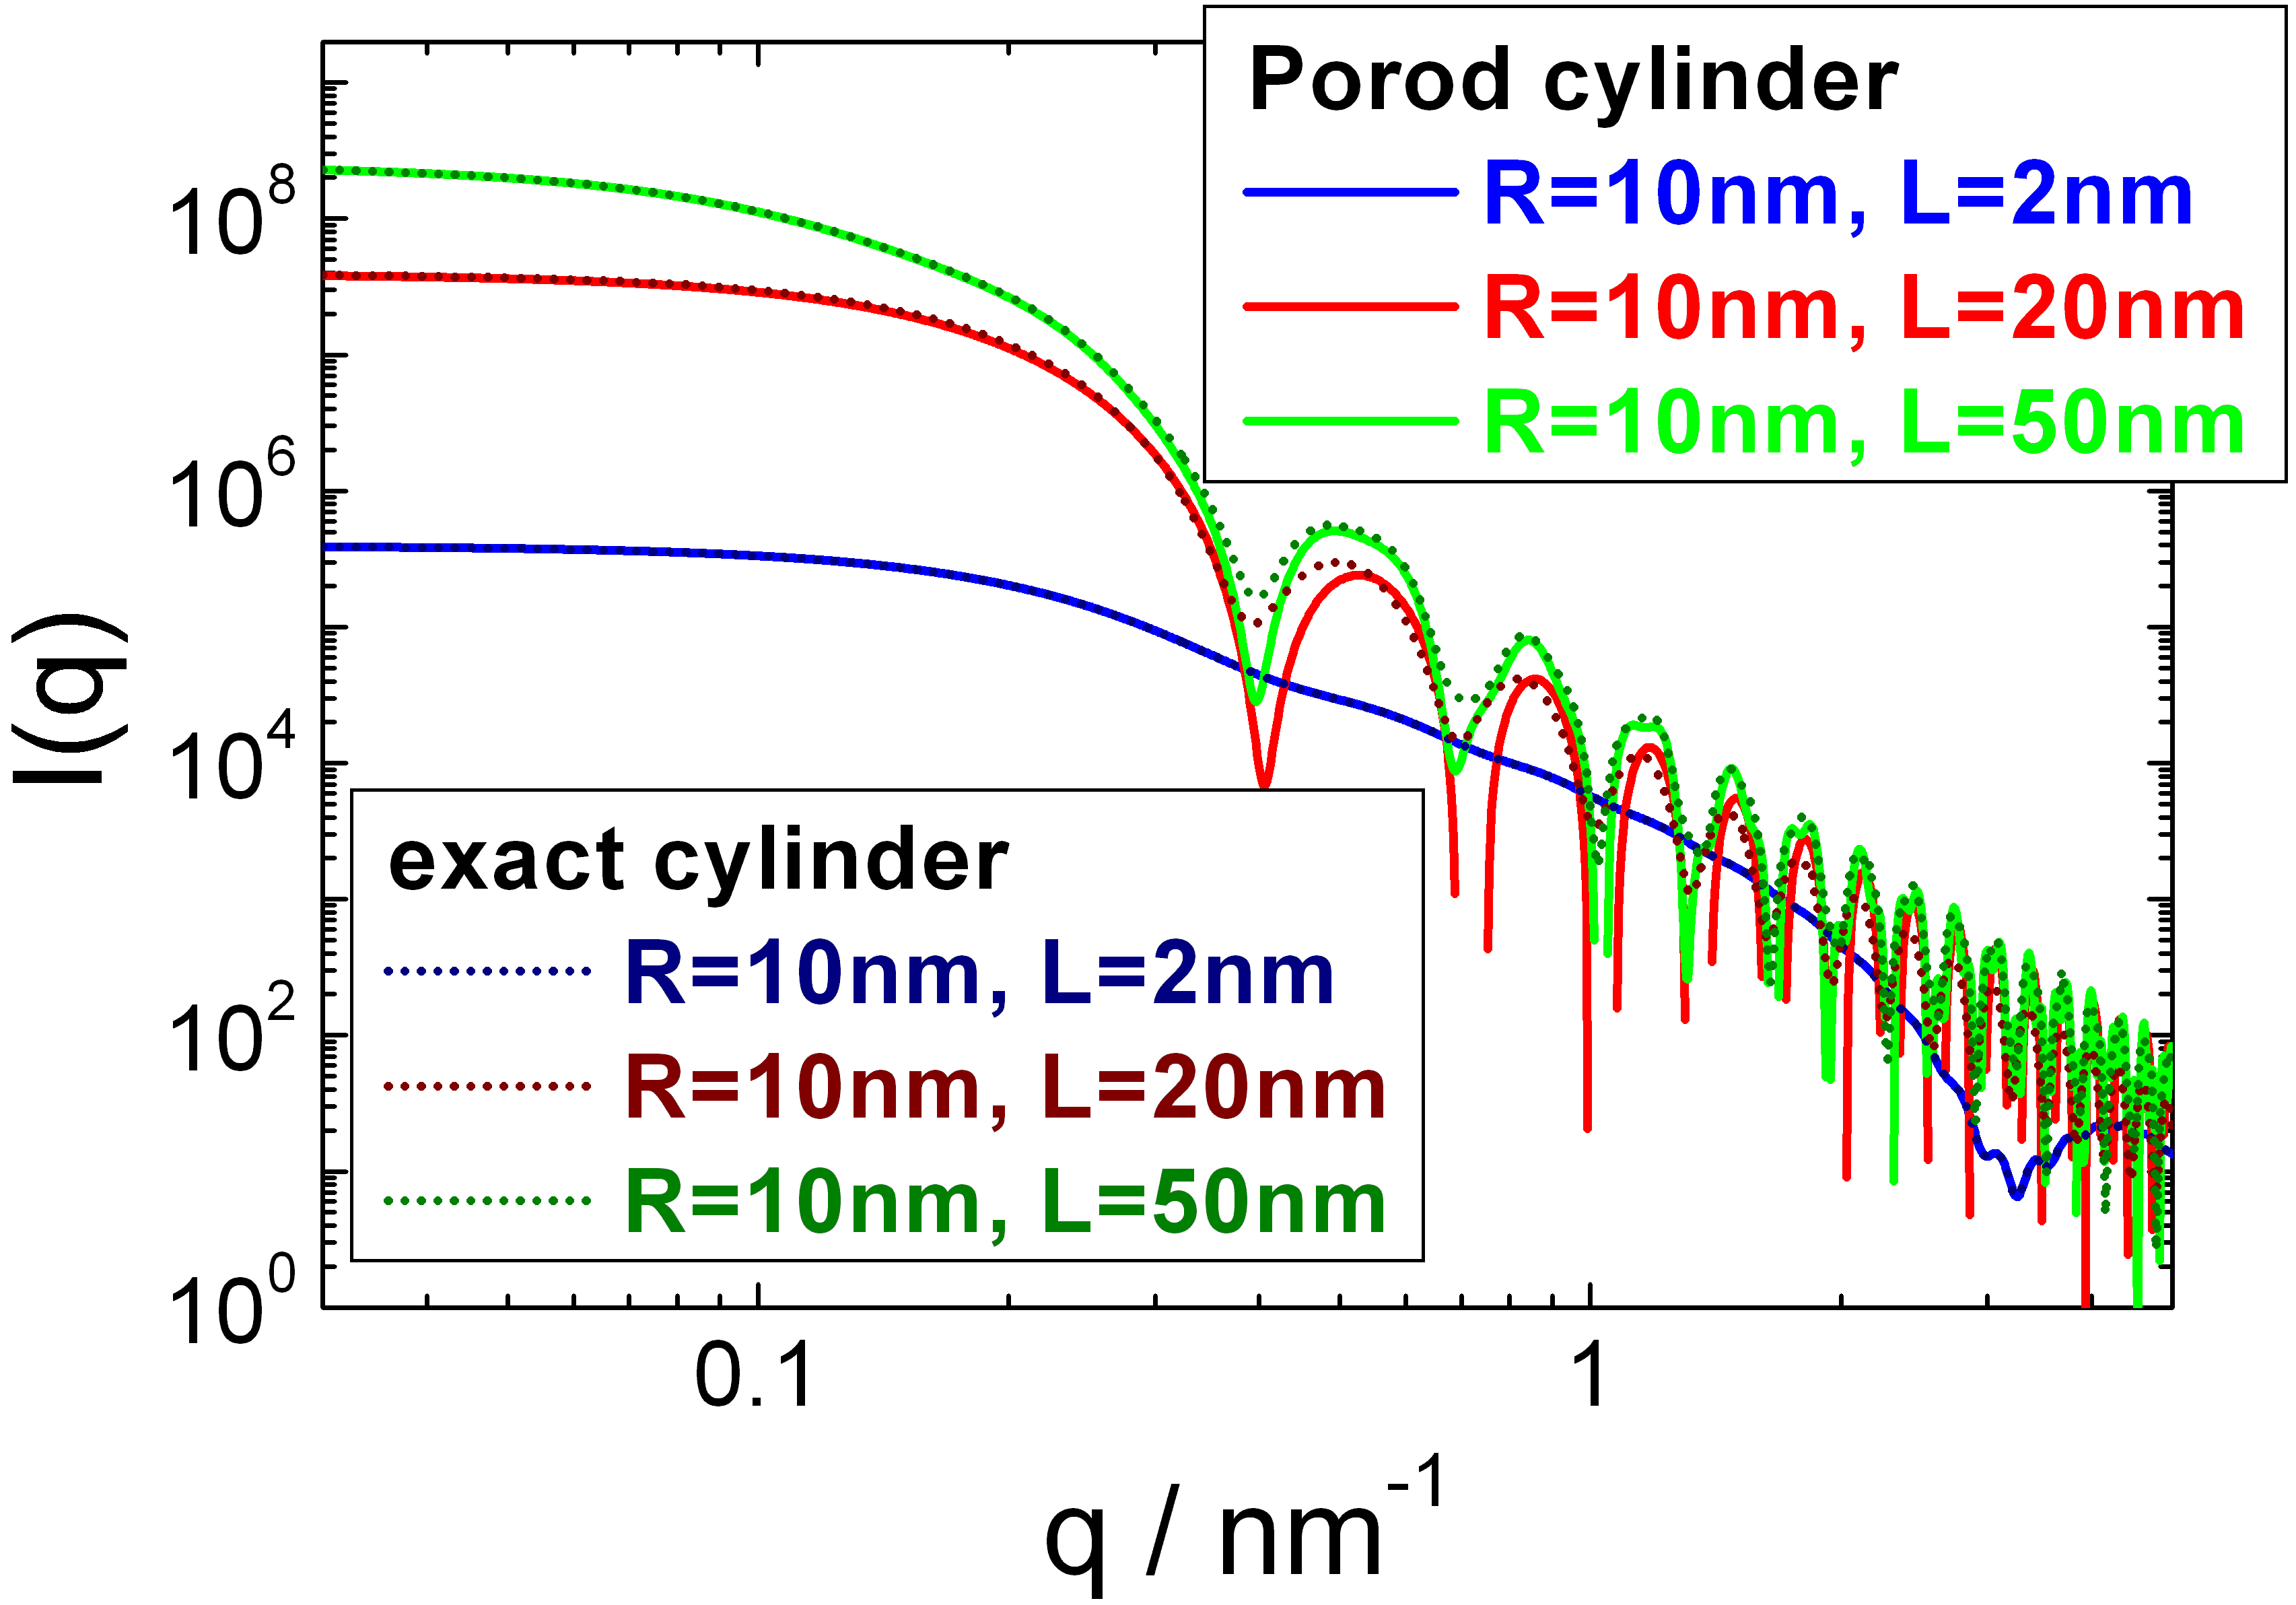
\includegraphics[width=0.55\textwidth]{../images/form_factor/cylindrical_obj/PorodCylinder.png}
\end{center}
\caption{Scattering intensity of a cylinder with radius $R=10$ nm and lengths of $L=2$ nm,
$L=20$ nm, and $L=50$ nm. Next to Porod's approximation for a cylinders also
the exact integral solution is shown for comparison.
The scattering length density contrast is set to 1.}
\label{fig:PorodCylinder}
\end{figure}
%%%%%%%%%%%%%%%%%%%%%%%%%%%%%%%%%%%%%%%%%%%%%%%%%%%%%%%%%%%%%%%%%%%%%%%%%%

\clearpage
\subsection{Cylinder of length $L$, radius $R$ and scattering
contrast $\Delta\eta$}
\label{sect:Cylinder}
~\\

\begin{figure}[htb]
\begin{center}
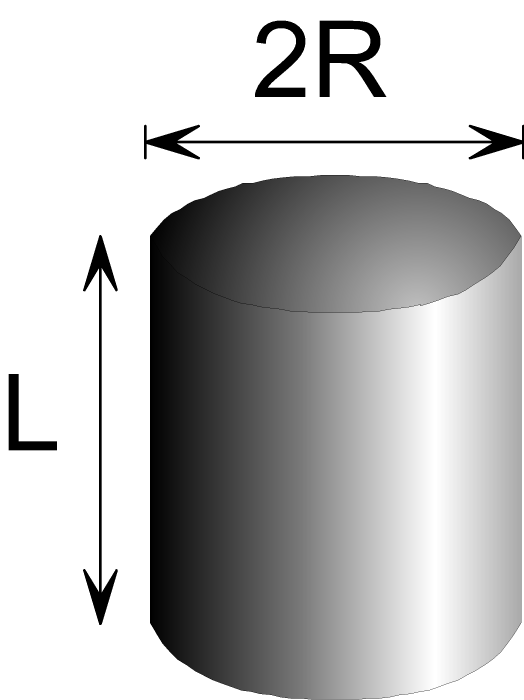
\includegraphics[width=0.192\textwidth]{../images/form_factor/cylindrical_obj/cylinder.png}
\end{center}
\caption{} \label{fig:cylinder}
\end{figure}
\begin{align}
I_\text{cyl} = 16 (\pi R^2 L)^2 \Delta\eta^2 \int_0^1 \left(
\frac{J_1\left(Q R \sqrt{1-x^2}\right)
                         \sin(Q L x/2)}{Q^2 R \sqrt{1-x^2} L x}
                      \right)^2 dx
\end{align}
\vspace{5mm}

\uline{Input Parameters for model \texttt{Cylinder}:}
\begin{description}
\item[\texttt{R}] radius of cylinder $R$
\item[\texttt{L}] length of cylinder $L$
\item[\texttt{eta}] scattering contrast $\Delta\eta$
\end{description}

\uline{Note:}
\begin{itemize}
\item None
\end{itemize}

\begin{figure}[htb]
\begin{center}
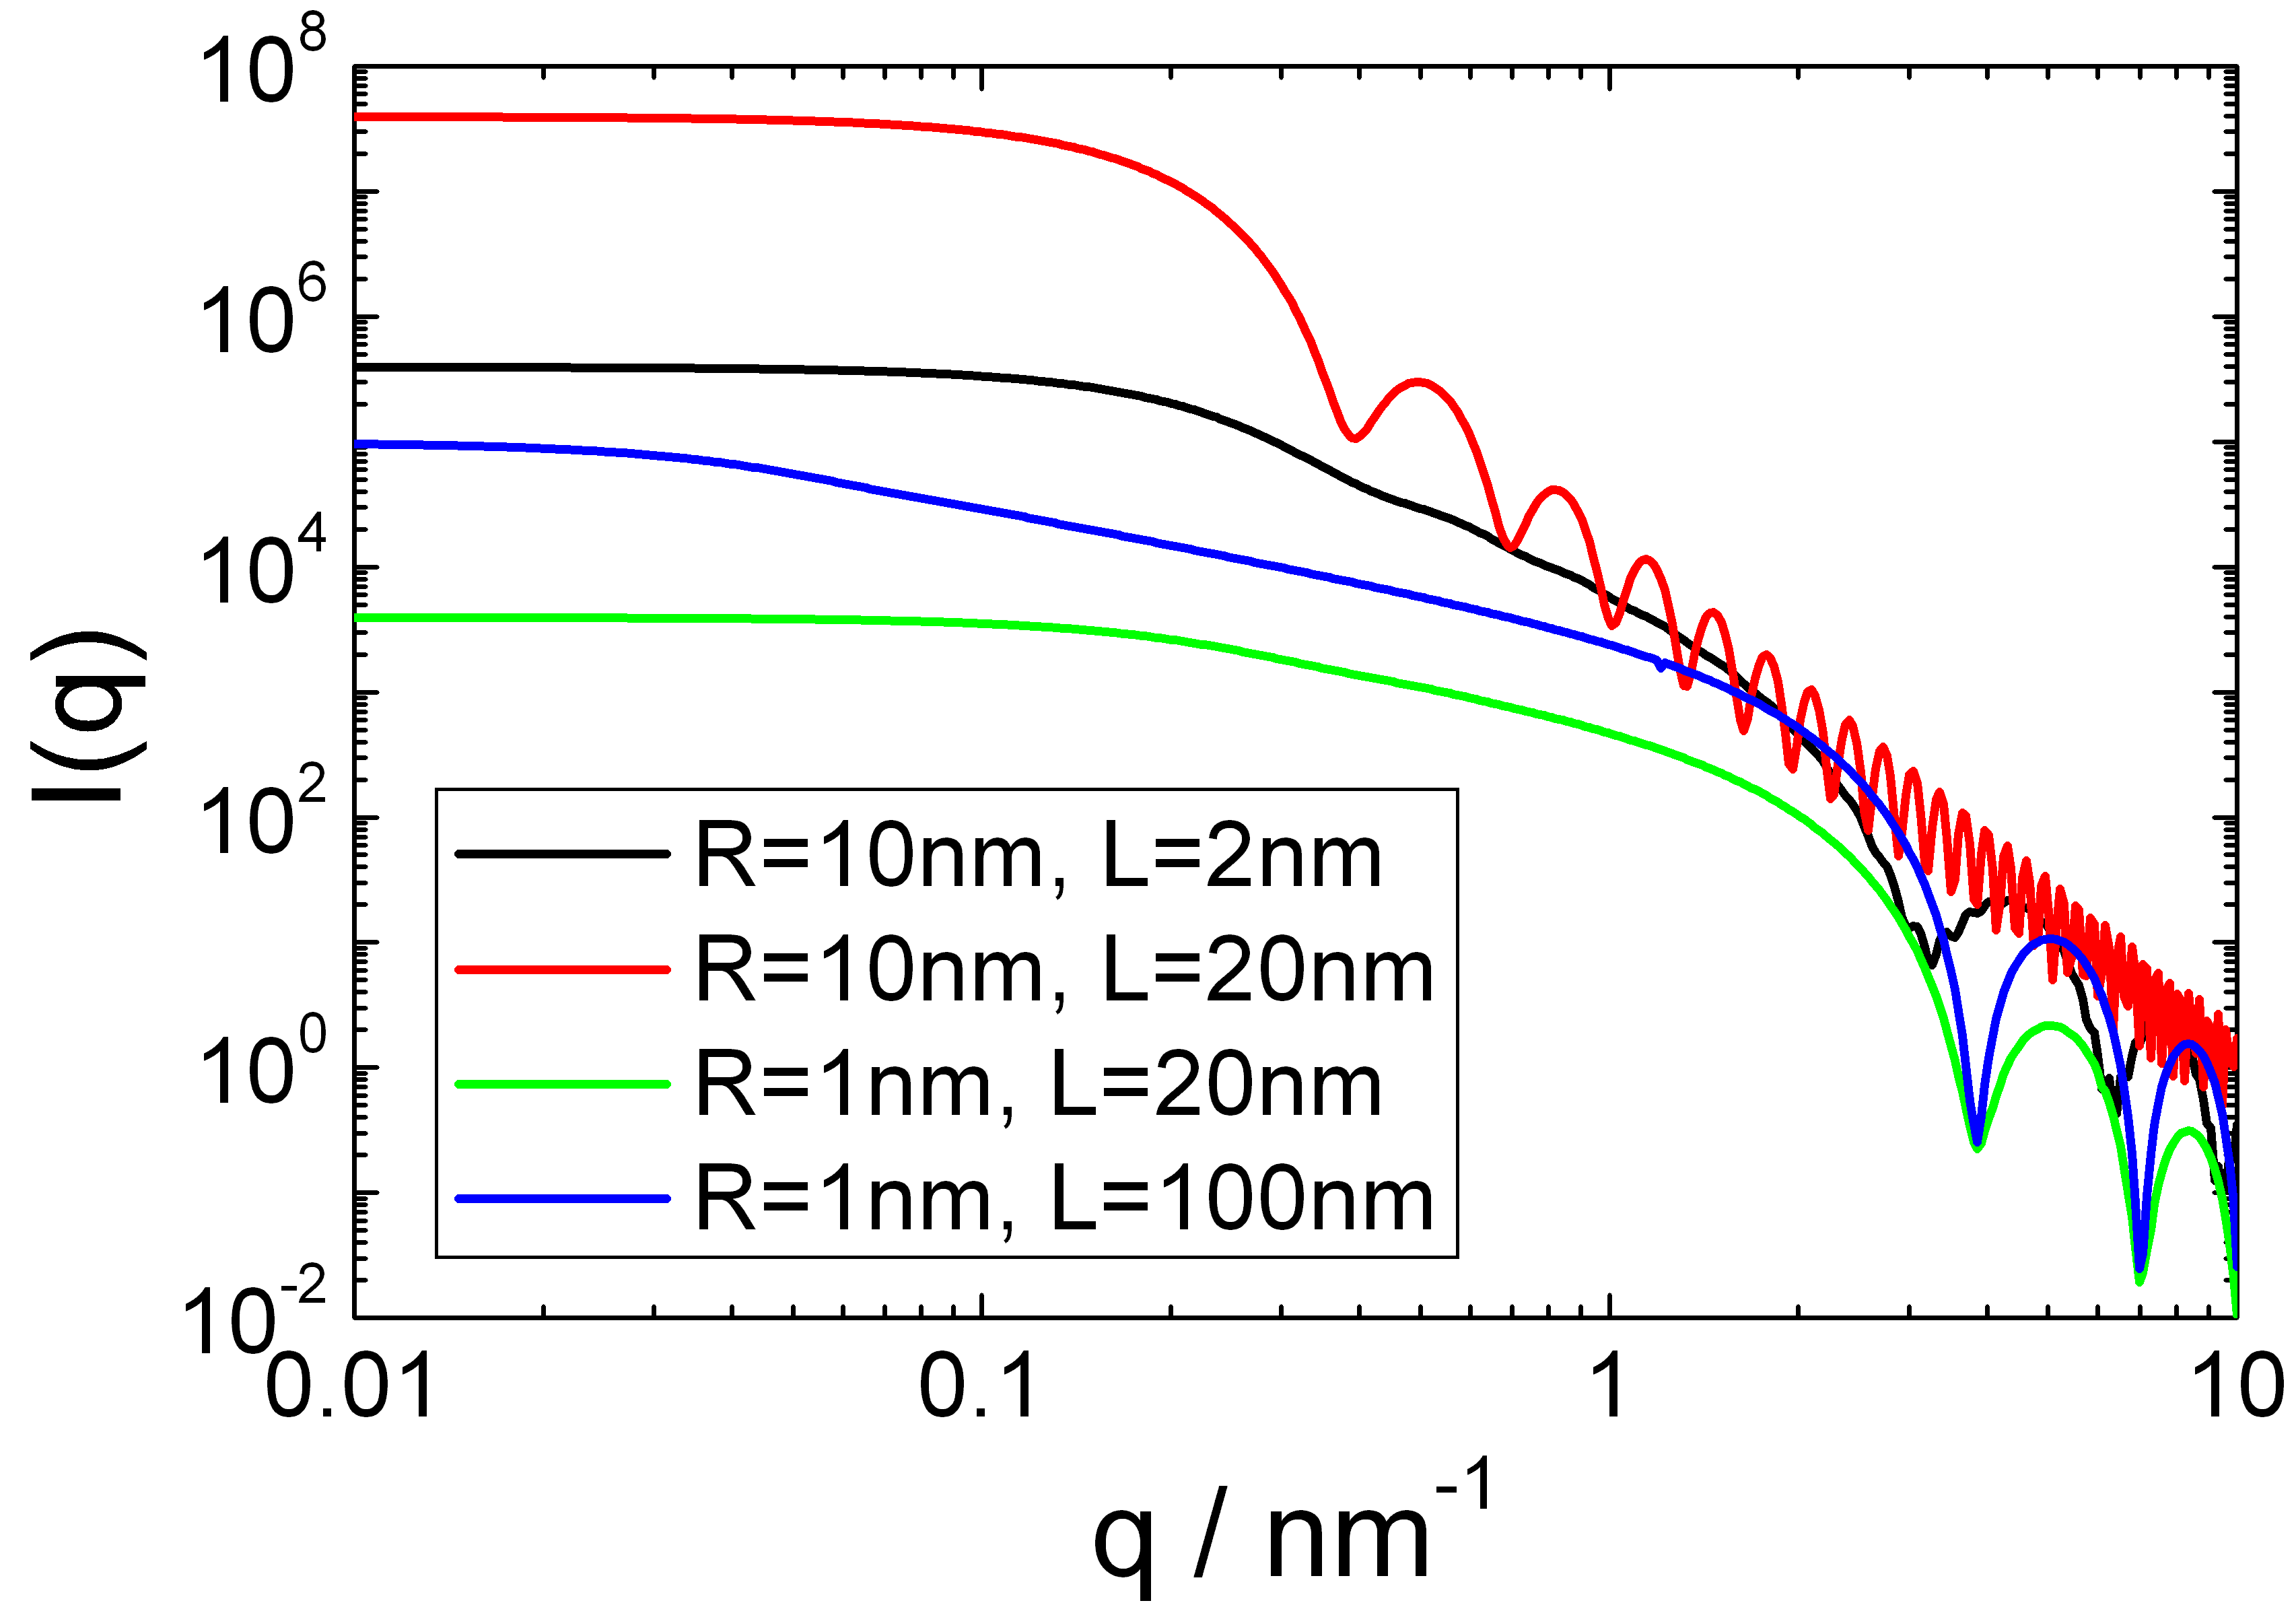
\includegraphics[width=0.55\textwidth]{../images/form_factor/cylindrical_obj/ExactCylinder.png}
\end{center}
\caption{Scattering intensity of a cylinder for different radii radius $R$ nm and lengths $L$.
The scattering length density contrast is set to 1.}
\label{fig:ExactCylinder}
\end{figure}

%%%%%%%%%%%%%%%%%%%%%%%%%%%%%%%%%%%%%%%%%%%%%%%%%%%%%%%%%%%%%%%%%%%%%%%%%%

\clearpage
\subsection{Random oriented cylindrical shell with circular cross-section}
\label{sect:randomCylindricalShell}
~\\

\begin{figure}[htb]
\begin{center}
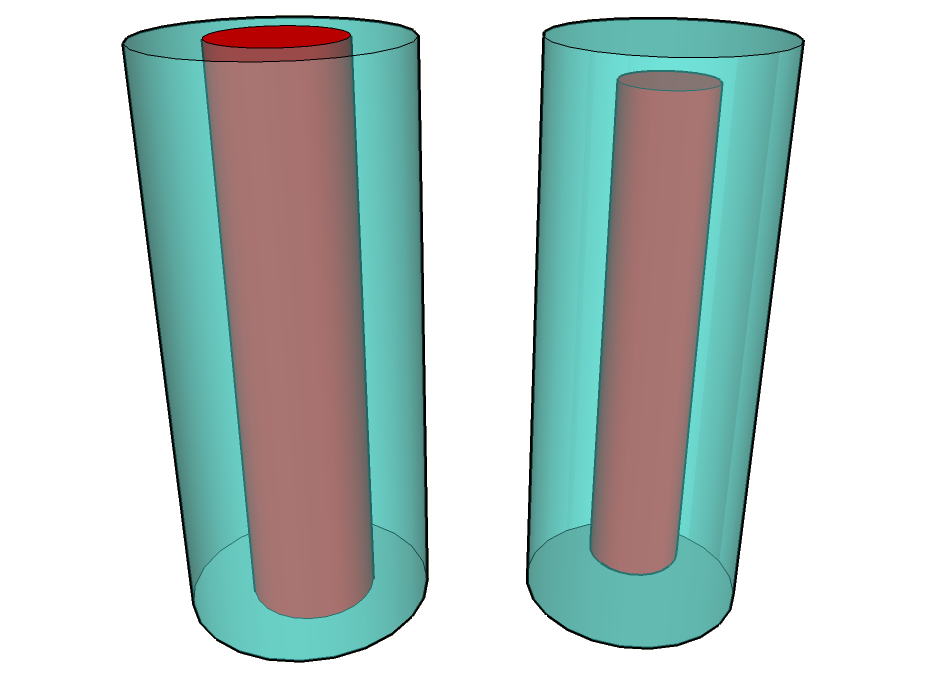
\includegraphics[width=0.4\textwidth]{../images/form_factor/cylindrical_obj/CylShell.png}
\hspace{0.1\textwidth}
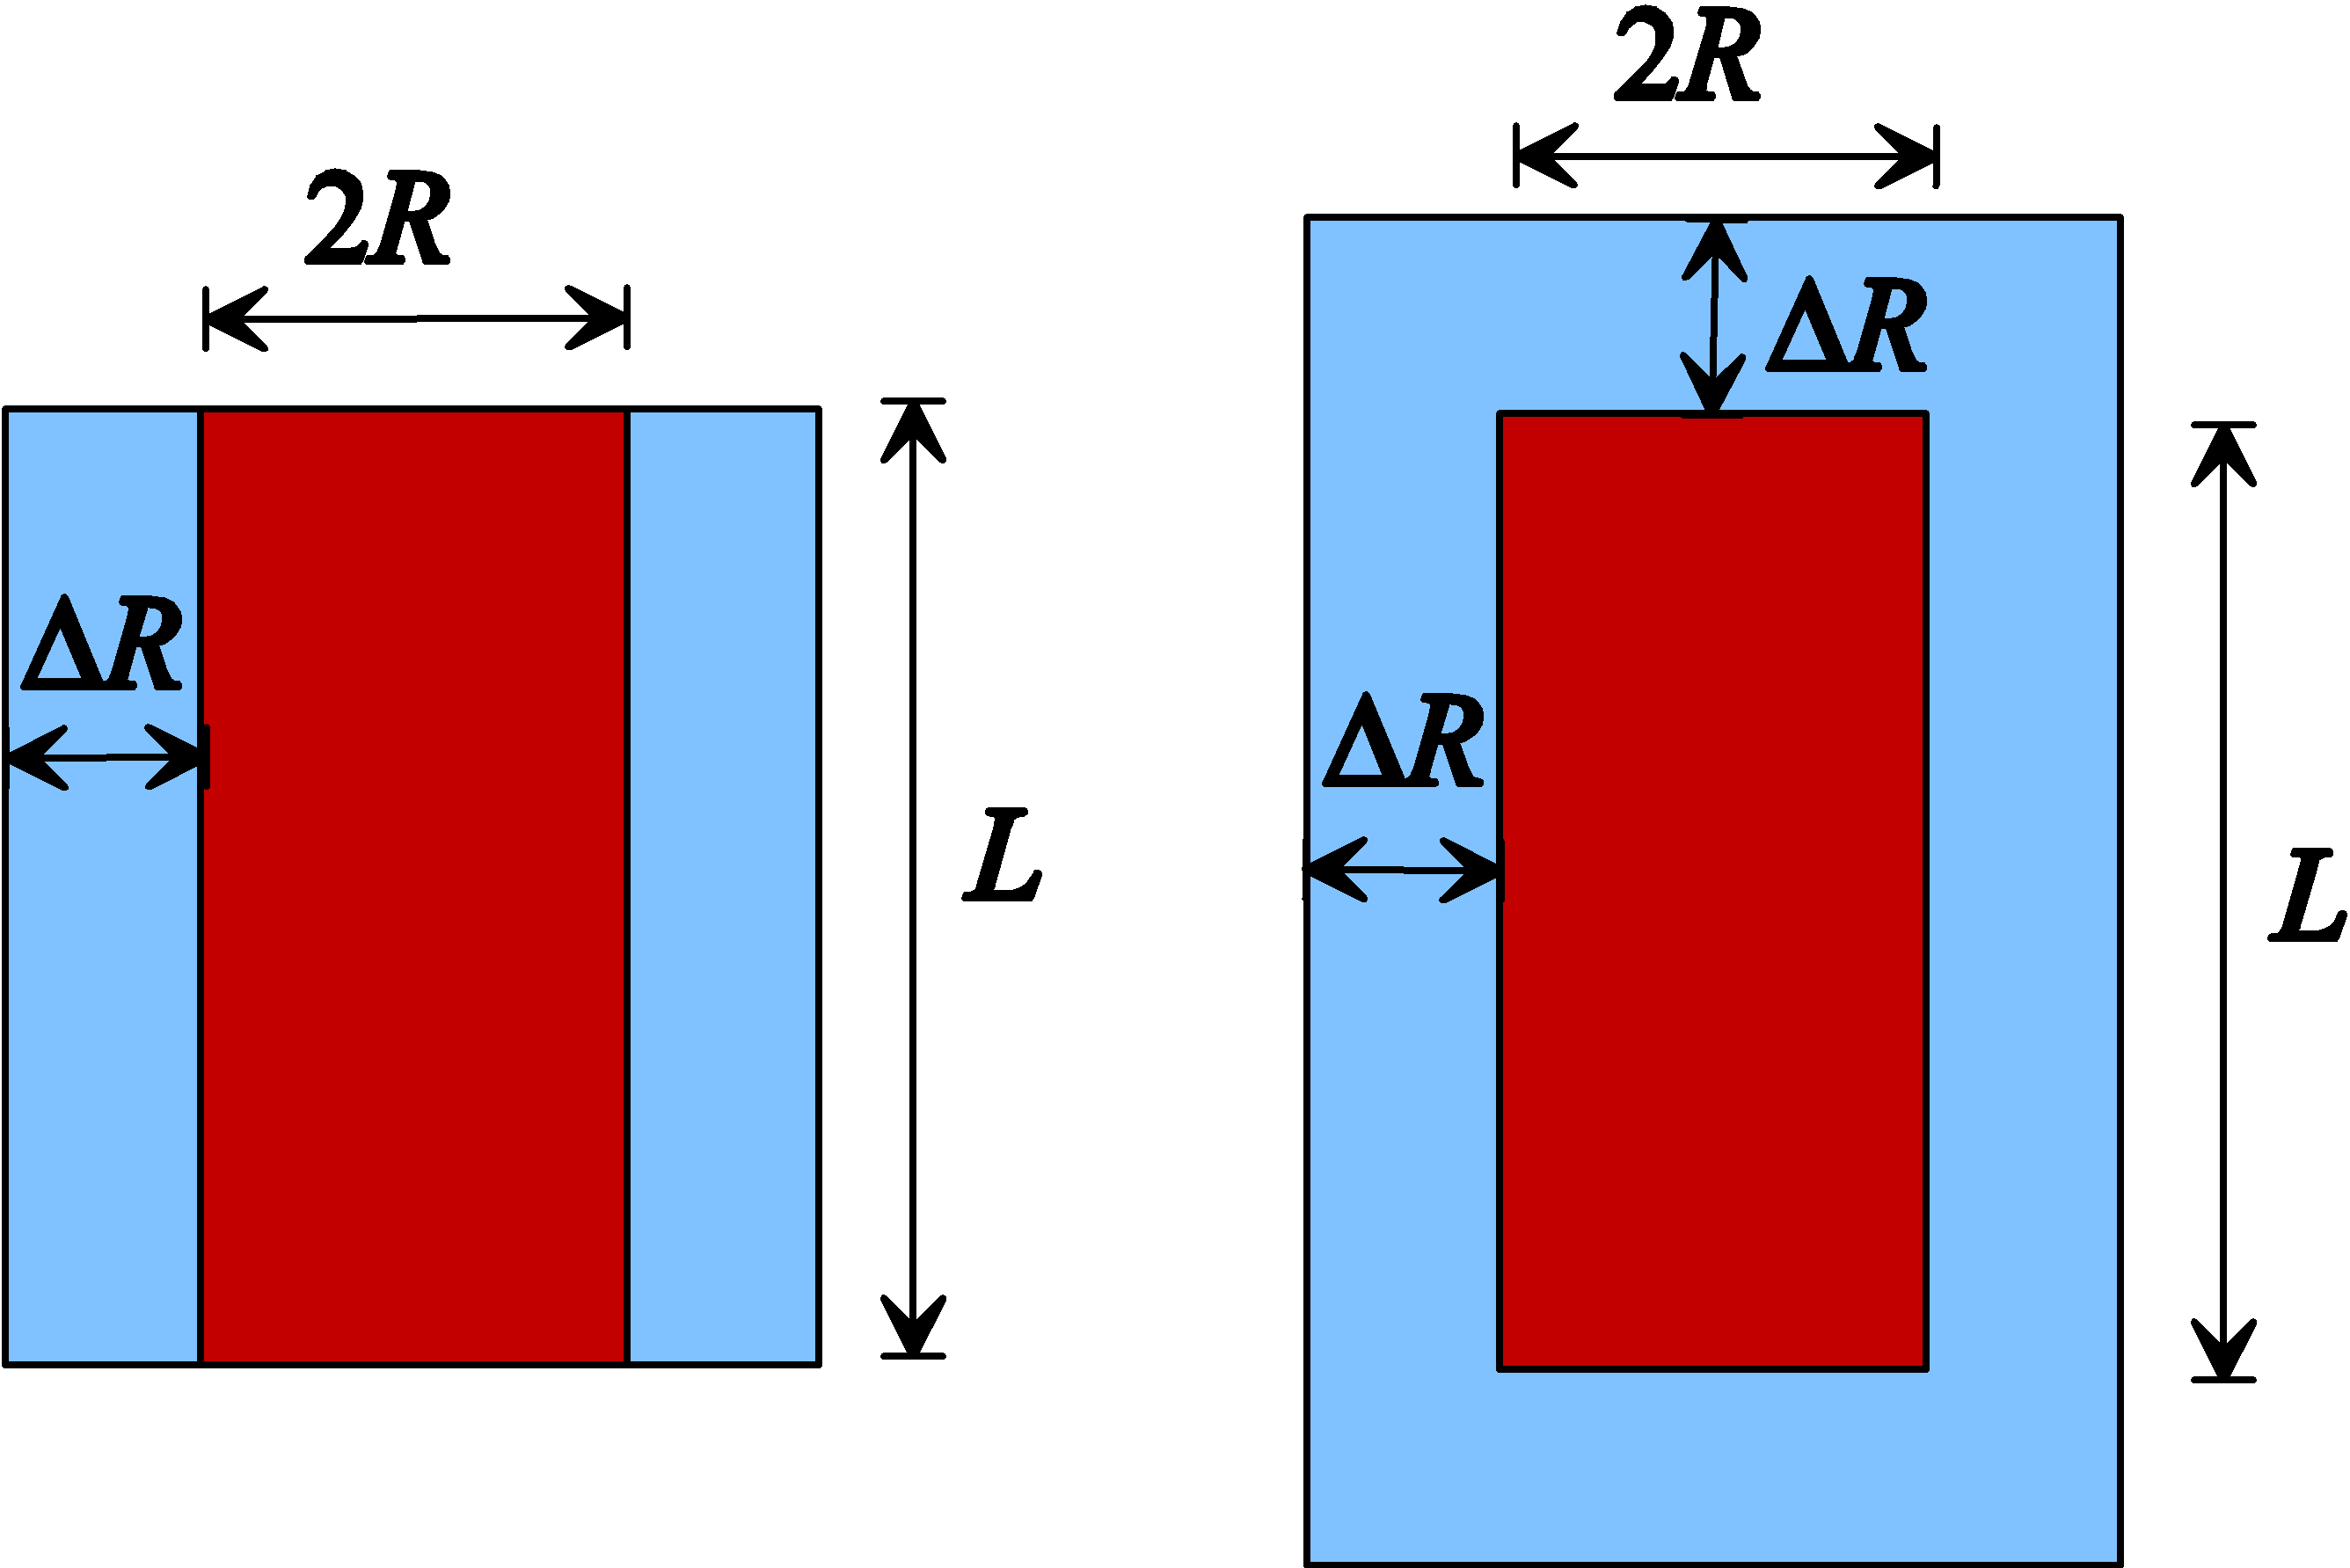
\includegraphics[width=.4\textwidth]{../images/form_factor/cylindrical_obj/cylshell2D.png}
\end{center}
\caption{cylindrical shell with circular cross-section}
\label{cylshell}
\end{figure}

To different versions for a random oriented cylindrical shell with a
circular cross-section has been implemented. One without  \texttt{CylShell1}
and one with \texttt{CylShell2} capped flat ends. For very long cylinders a faster
approximation for the uncapped version can be used \texttt{LongCylShell}

\begin{align}
K_\text{Cyl}(Q,\Delta\eta,R,L,x) =
2 \pi R^2 L \Delta \eta
    \frac{J_1\left(Q R \sqrt{1-x^2}\right)}{Q R \sqrt{1-x^2}}
    \frac{\sin(Q L x/2)}{QL x/2}
\end{align}

\begin{align}
I_\text{CylShell1} =
\int_0^1 \biggl(
  &
  K_\text{Cyl}\left(Q,\eta_\text{core}-\eta_\text{shell},R,L,x\right) \\
+&  K_\text{Cyl}\left(Q,\eta_\text{shell}-\eta_\text{solv},R+t,L,x\right)
\biggr)^2 dx \nonumber \\
I_\text{CylShell2} =
\int_0^1 \biggl(
 &  K_\text{Cyl}\left(Q,\eta_\text{core}-\eta_\text{shell},R,L,x\right) \\
+&  K_\text{Cyl}\left(Q,\eta_\text{shell}-\eta_\text{solv},R+t,L+2t,x\right)
\biggr)^2 dx \nonumber
\end{align}

\begin{align}
  I_\text{LongCylShell}(Q) = & P'(Q) P_\text{cs}(Q) \\
  P'(Q)  = & 2 \frac{\text{Si}(Q L)}{QL} - \left(\frac{\sin(QL/2)}{QL/2}\right)^2 \\
  \text{Si}(x) & = \int_0^x\!\frac{\sin t}{t}\,\,dt \\
  P_\text{cs}(Q)  =  & \biggl(
            2\frac{J_1(QR)}{QR}
            \left(\eta_\text{core}-\eta_\text{shell}\right)R^2L\pi + \\
         & \qquad
            2\frac{J_1(Q(R+t))}{Q(R+t)}
            \left(\eta_\text{shell}-\eta_\text{solv}\right)(R+t)^2L\pi
      \biggr)^2  \nonumber
\end{align}


\vspace{5mm}

\hspace{1pt}\\
\uline{Input Parameters for models \texttt{CylShell1}, \texttt{CylShell2} and \texttt{LongCylShell}:}\\
\begin{description}
\item[\texttt{R}] core radius $R$
\item[\texttt{t}] shell thickness $t$
\item[\texttt{L}] cylinder length $L$
\item[\texttt{eta\_core}] scattering length density $\eta_\text{core}$ of cylinder core
\item[\texttt{eta\_shell}] scattering length density $\eta_\text{shell}$ of cylinder shell
\item[\texttt{eta\_solv}] scattering length density $\eta_\text{solv}$ of solvent
\end{description}

\uline{Note:}
\begin{itemize}
\item The approximation for a long cylindrical shell (\texttt{LongCylShell}) only holds for $L \gg 2R$.
\end{itemize}

\begin{figure}[htb]
\begin{center}
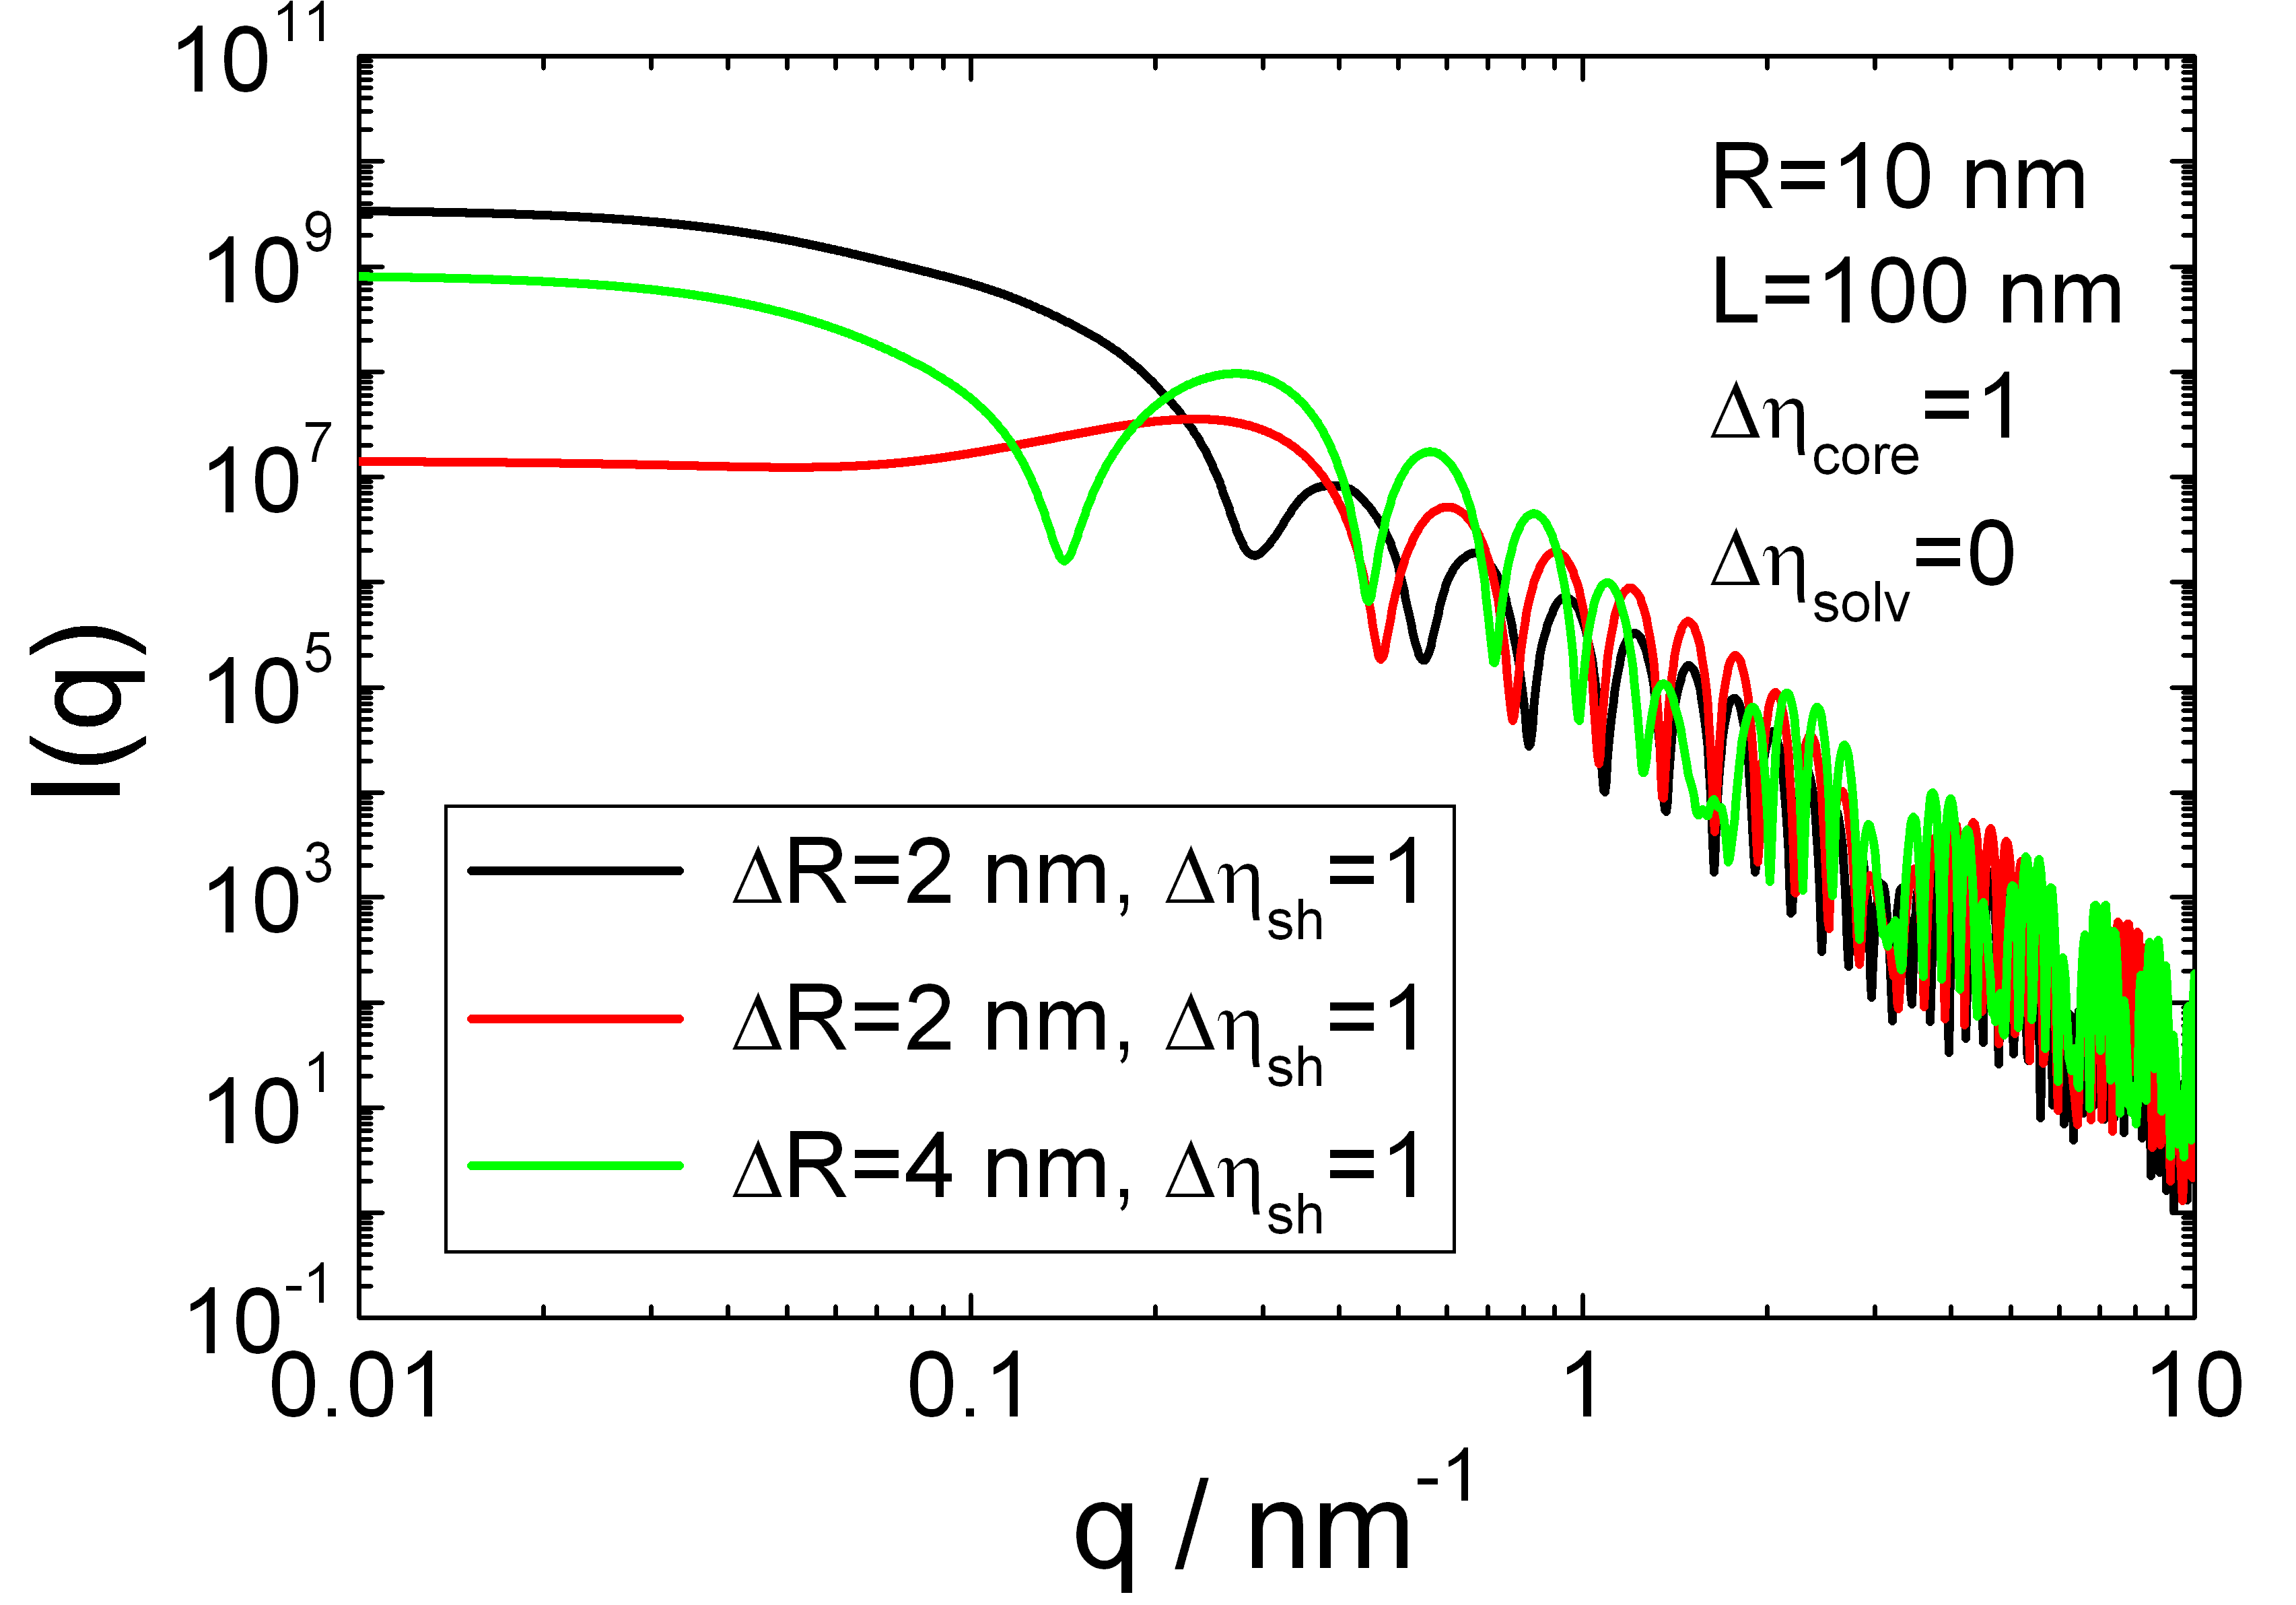
\includegraphics[width=0.55\textwidth]{../images/form_factor/cylindrical_obj/CylShell1IQ.png}
\end{center}
\caption{Scattering intensity of a cylinder shell \texttt{CylShell1}.}
\label{fig:CylShell1}
\end{figure}

\begin{figure}[htb]
\begin{center}
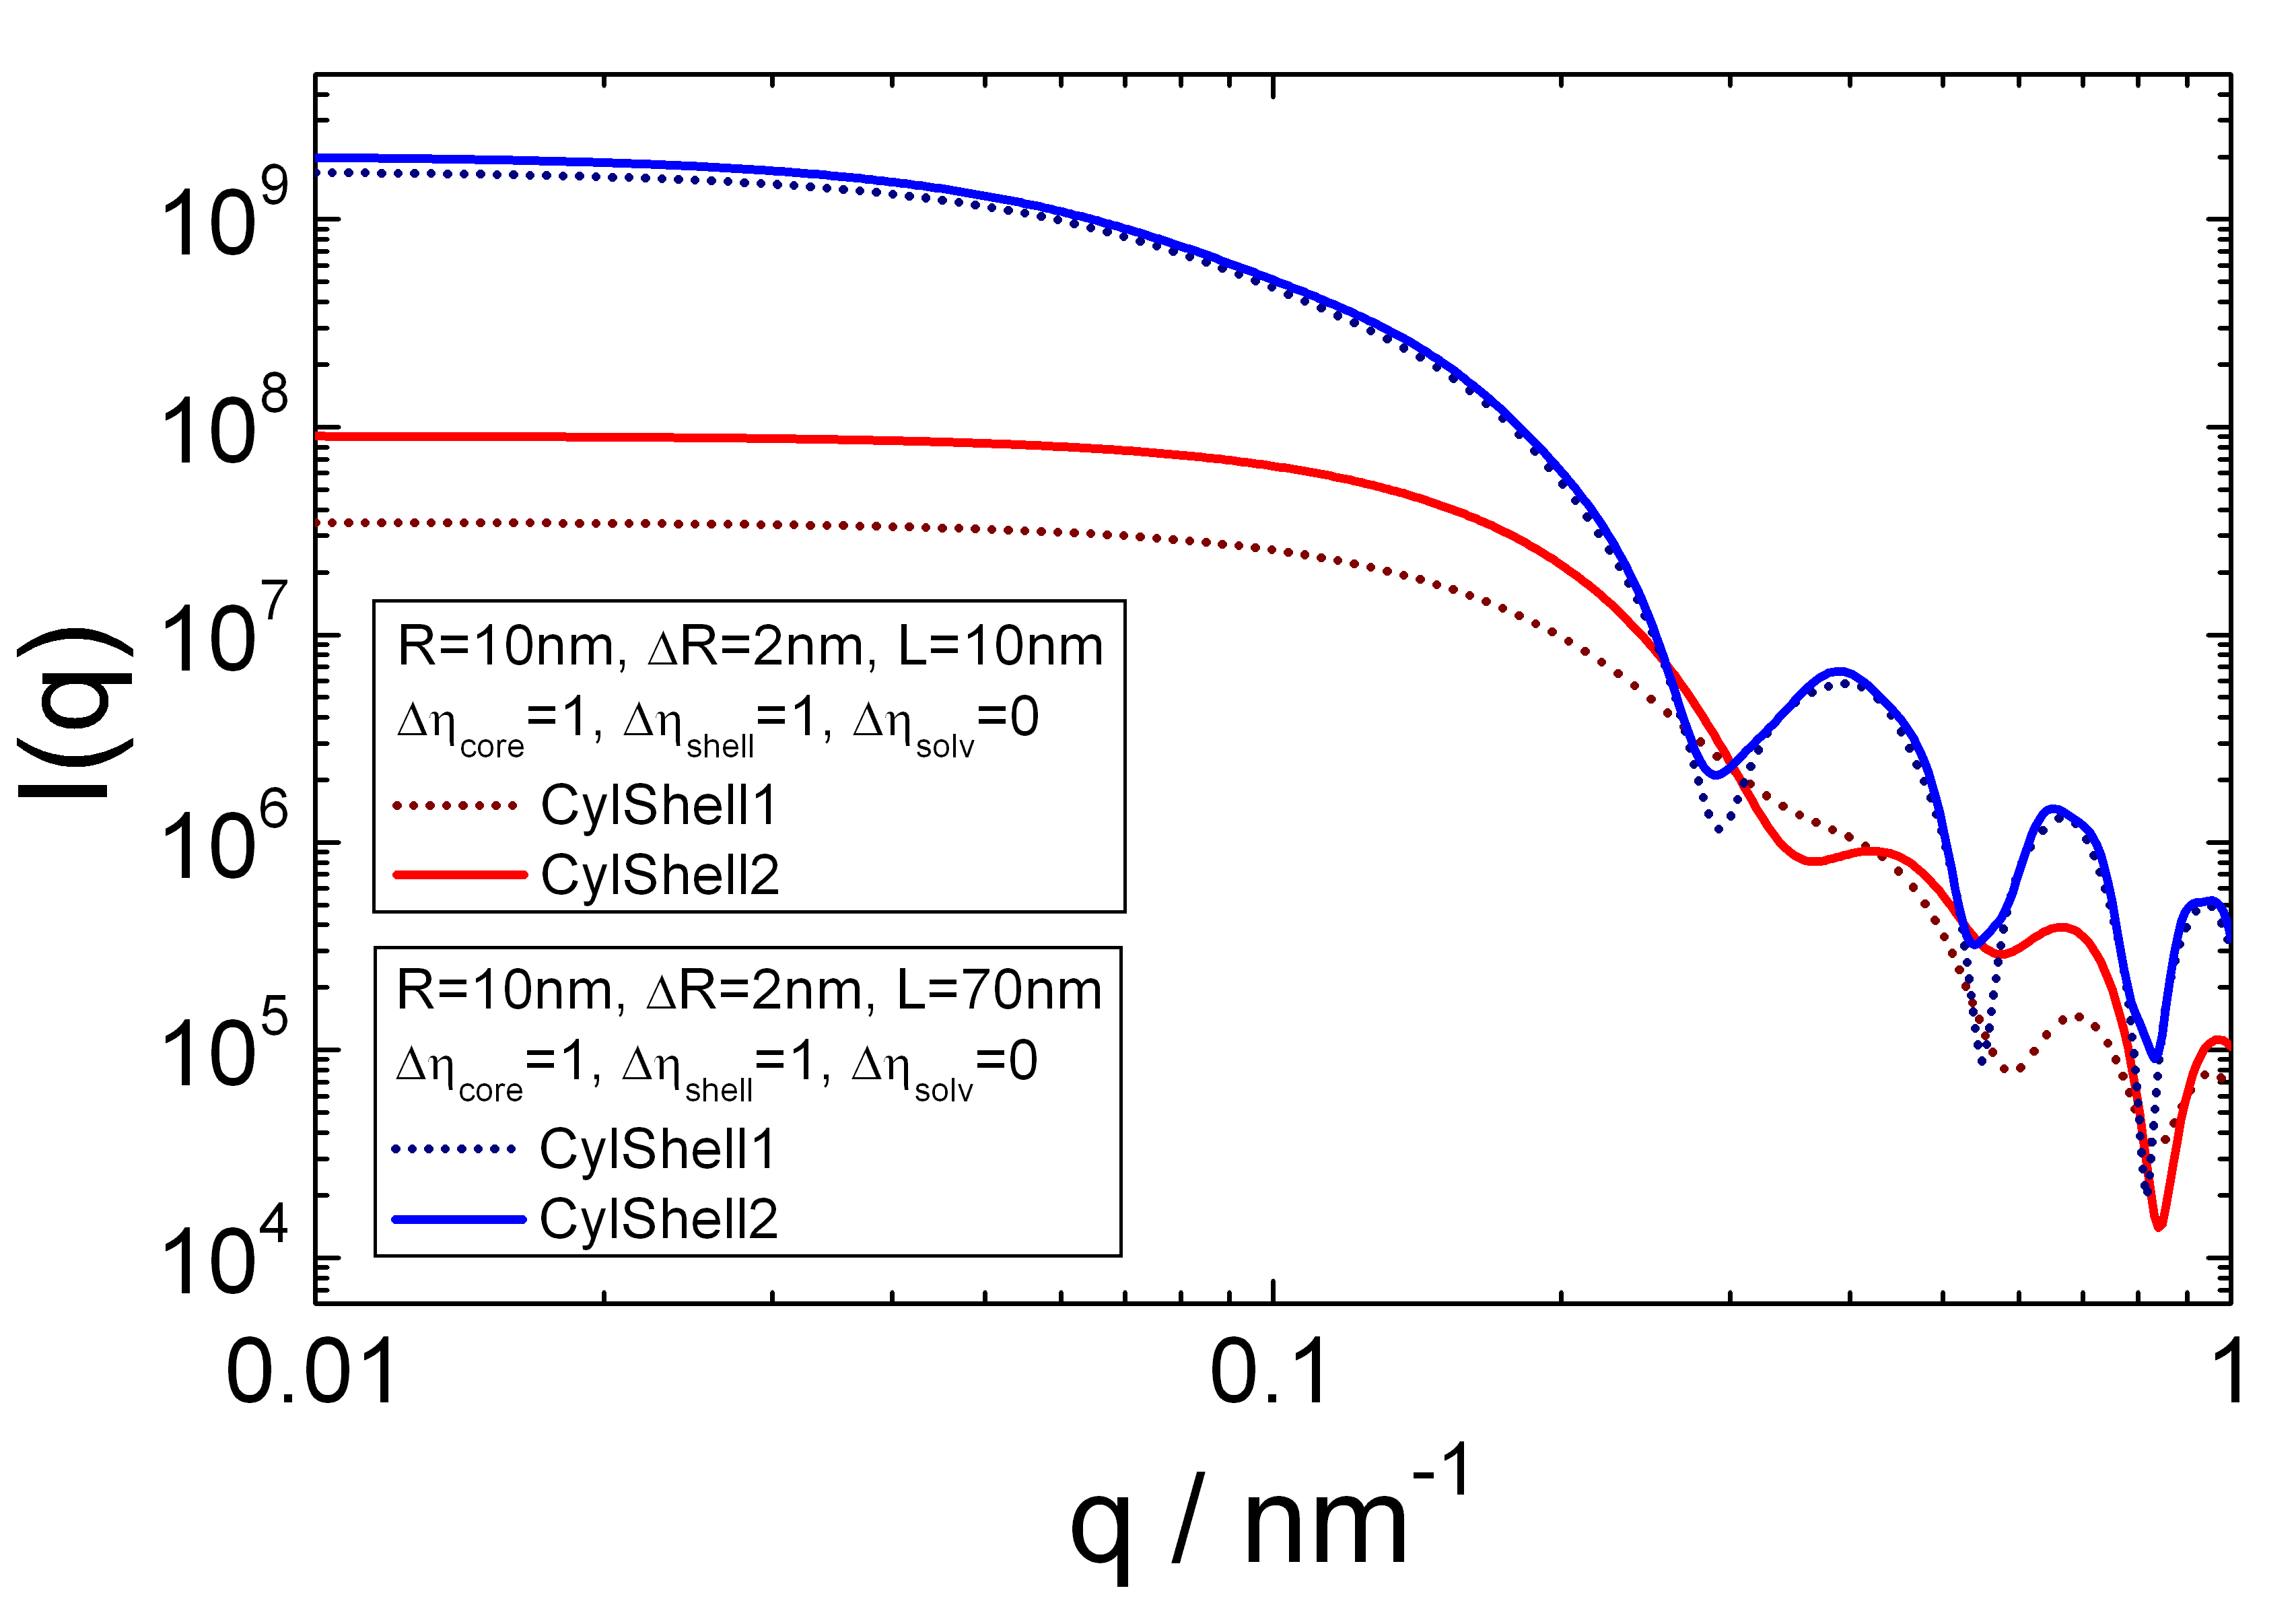
\includegraphics[width=0.55\textwidth]{../images/form_factor/cylindrical_obj/CylShell2IQ.png}
\end{center}
\caption{Scattering intensity of a cylinder shell \texttt{CylShell2}.}
\label{fig:CylShell2}
\end{figure}


%%%%%%%%%%%%%%%%%%%%%%%%%%%%%%%%%%%%%%%%%%%%%%%%%%%%%%%%%%%%%%%%%%%%%%%%%%%%%%%%%%%%%%%%%%%%

\clearpage
\subsection{Random oriented cylindrical shell with elliptical cross-section}
\label{sect:random_ellCylinderShell}
~\\

\begin{figure}[htb]
\begin{center}
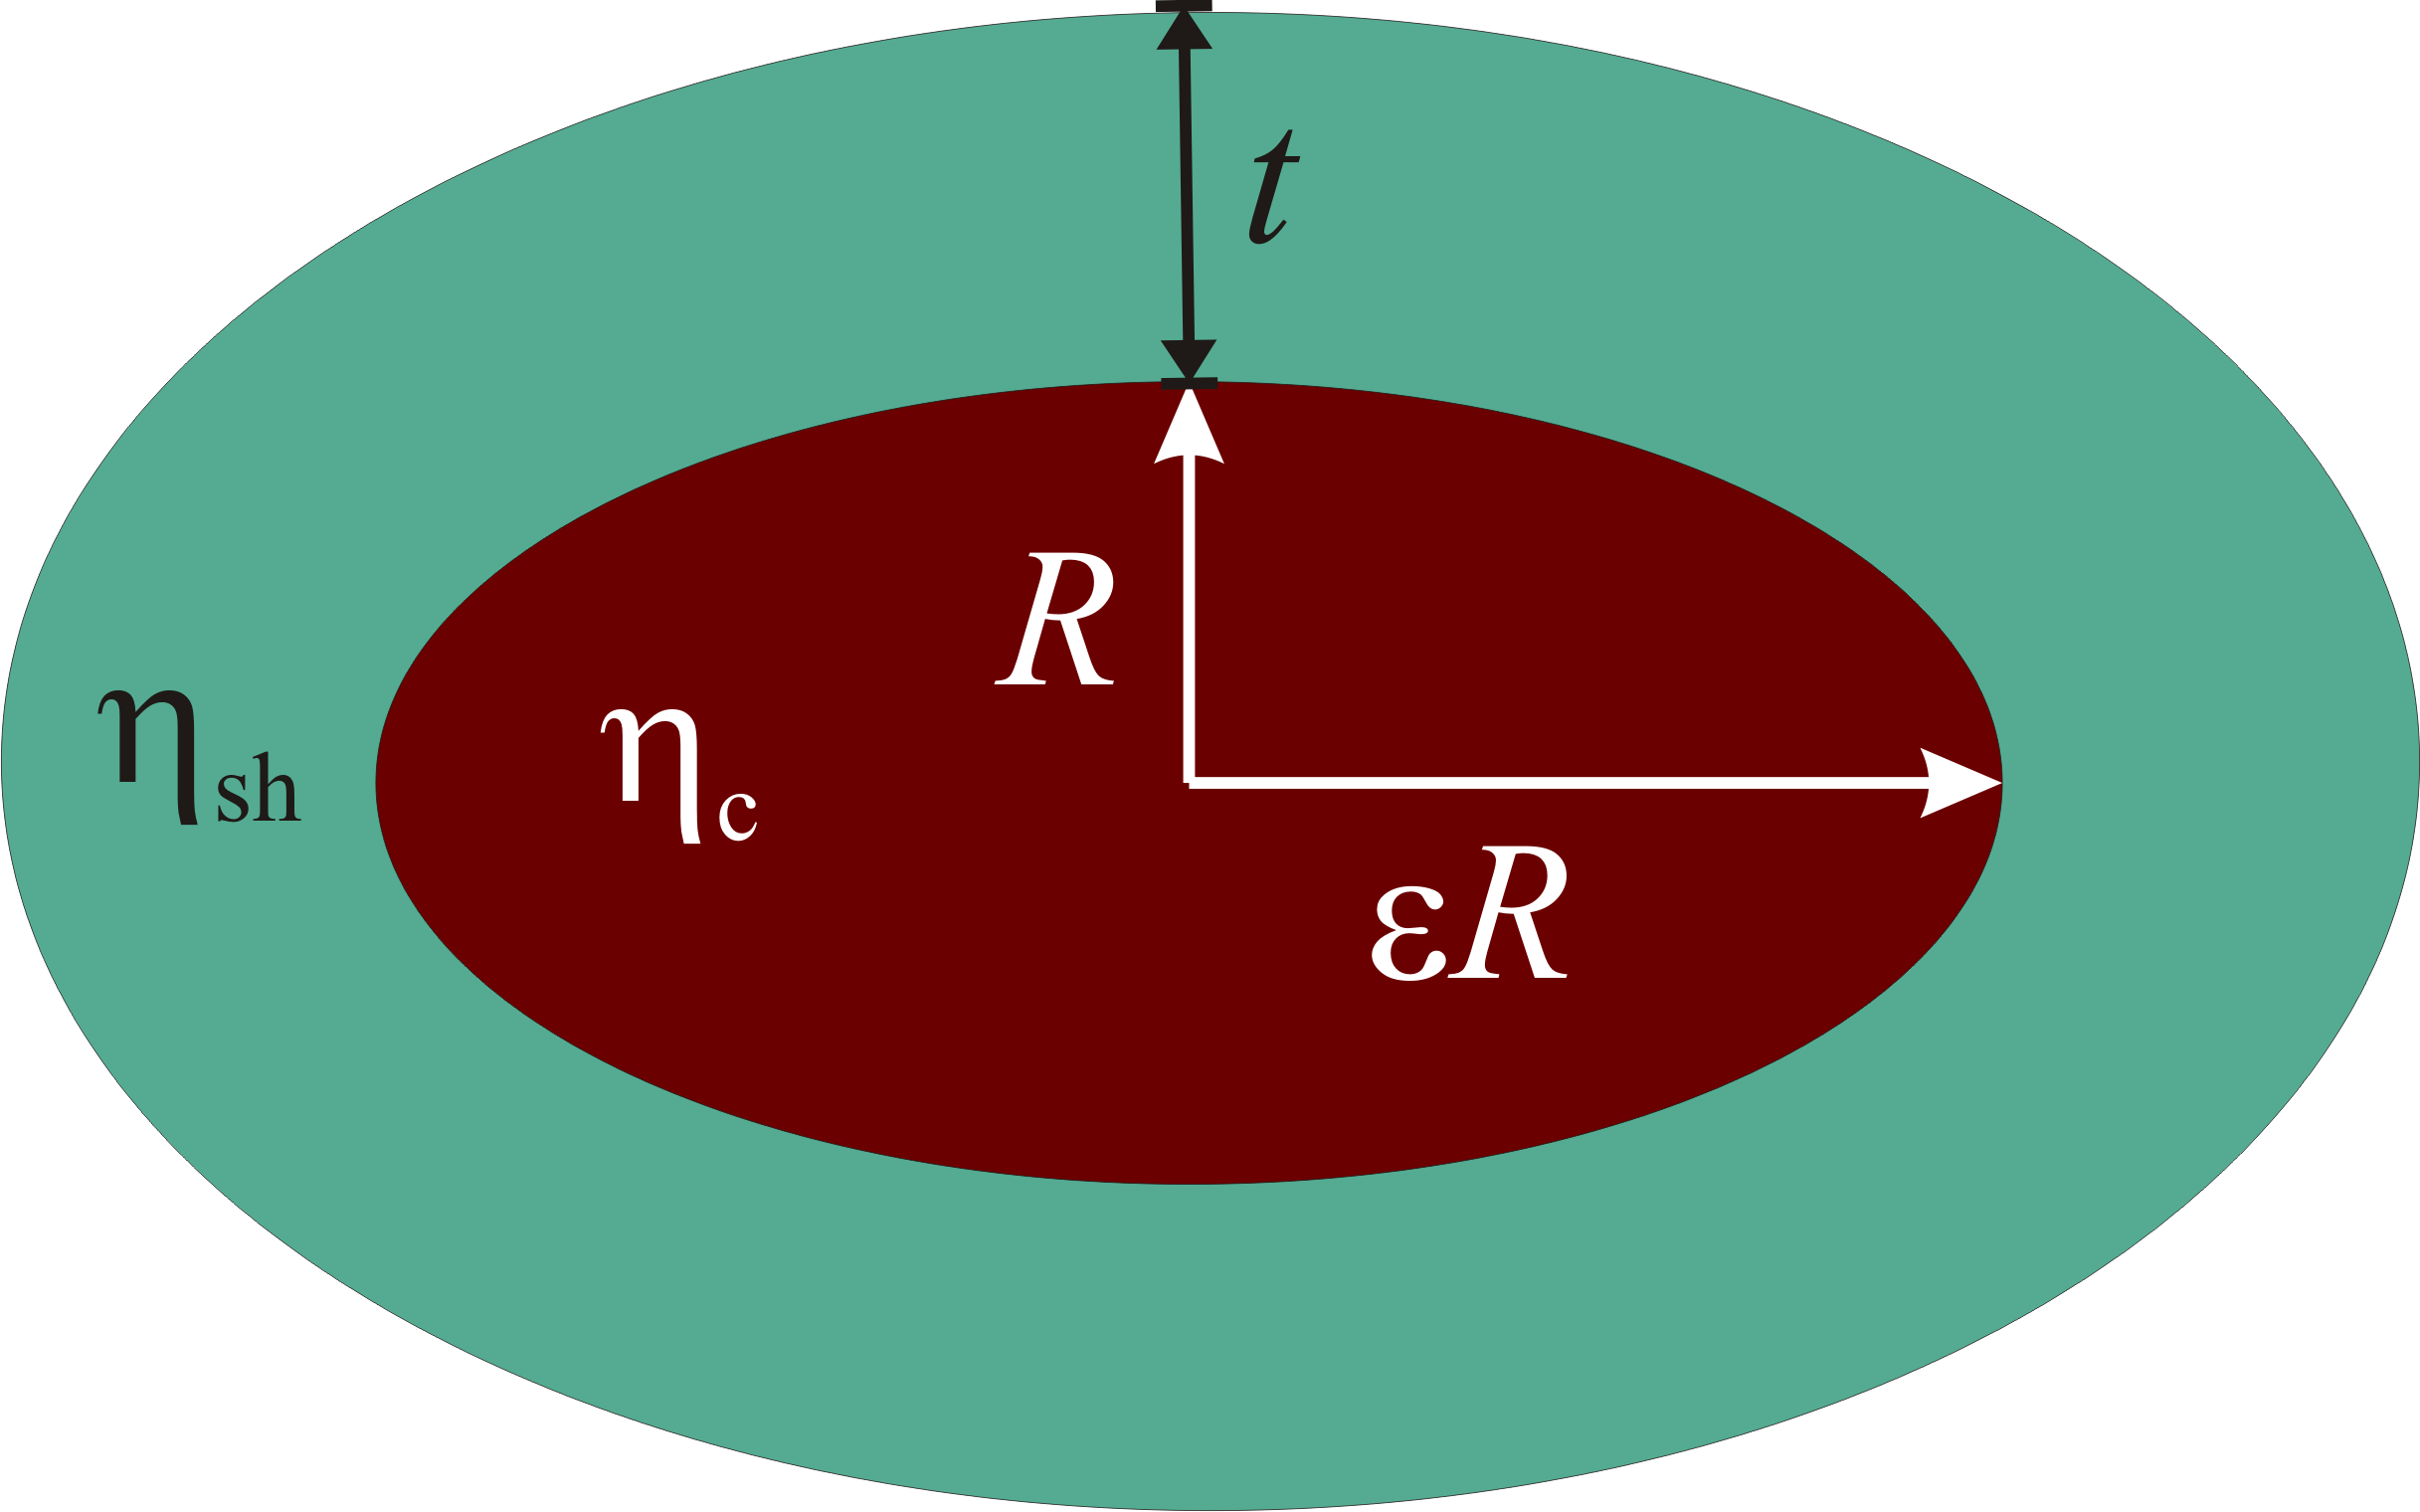
\includegraphics[width=0.4866\textwidth]{../images/form_factor/cylindrical_obj/ellCylShell_shape.png}
\hspace{0.0\textwidth}
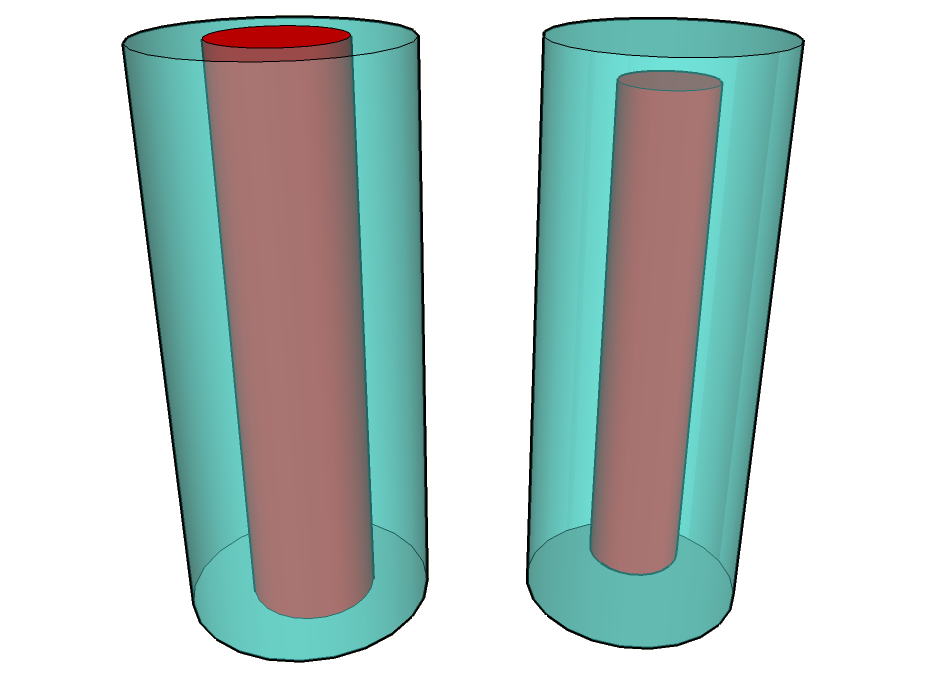
\includegraphics[width=0.4\textwidth]{../images/form_factor/cylindrical_obj/CylShell.png}
\end{center}
\caption{cylindrical shell with elliptical cross-section}
\label{fig:ellCylShell}
\end{figure}

To different versions for a random oriented cylindrical shell with
an elliptical cross-section has been implemented. One without
\texttt{ellCylShell1} and one with \texttt{ellCylShell2} capped flat
ends.

\begin{align}
K_\text{ellCyl}(q,\Delta\eta,R,\epsilon,L,t,\phi,\alpha) &= \pi \epsilon R(\epsilon R+t) L
\Delta \eta \\
    & \times \frac{2J_1\left(q r(R,\epsilon,t,\phi,\alpha) \right)}{q r(R,\epsilon,t,\phi,\alpha)}
    \frac{\sin(q \frac{L}{2}\cos(\alpha))}{q\frac{L}{2}\cos(\alpha)} \nonumber \\
r(R,\epsilon,t,\phi,\alpha) &= \sqrt{(R+t)^2\sin^2(\phi)+(\epsilon R+t)^2\cos^2(\phi)}
\end{align}

\begin{align}
I_\text{ellCylShell1}(q) = \frac{2}{\pi}\int_0^{\frac{\pi}{2}} \!\! \int_0^{\frac{\pi}{2}} \biggl(
  &
  K_\text{ellCyl}\left(q,\eta_\text{core}\mathord-\eta_\text{shell},R,\epsilon,L,0,\phi,\alpha\right) \\
+&  K_\text{ellCyl}\left(q,\eta_\text{shell}\mathord-\eta_\text{sol},R,\epsilon,L,t,\phi,\alpha\right)
\biggr)^2 \sin(\alpha) \,d\alpha\, d\phi \nonumber \\
I_\text{ellCylShell2}(q) = \frac{2}{\pi}\int_0^{\frac{\pi}{2}} \!\!  \int_0^{\frac{\pi}{2}}  \biggl(
 &  K_\text{ellCyl}\left(q,\eta_\text{core}\mathord-\eta_\text{shell},R,\epsilon,L,0,\phi,\alpha\right) \\
+&  K_\text{ellCyl}\left(q,\eta_\text{shell}\mathord-\eta_\text{sol},R,\epsilon,L\mathord+2t,t,\phi,\alpha\right) \biggr)^2 \sin(\alpha) \,d\alpha \,d\phi  \nonumber
\end{align}


\vspace{5mm}

\hspace{1pt}\\
\uline{Input Parameters for models \texttt{ellCylShell1} and \texttt{ellCylShell2}:}\\
\begin{description}
\item[\texttt{R}] core radius $R$
\item[\texttt{epsilon}] stretching factor $\epsilon$ of cross-section
\item[\texttt{L}] cylinder length $L$
\item[\texttt{t}] shell thickness $t$
\item[\texttt{eta\_core}] scattering length density $\eta_\text{core}$ of cylinder core
\item[\texttt{eta\_shell}] scattering length density $\eta_\text{shell}$ of cylinder shell
\item[\texttt{eta\_sol}] scattering length density $\eta_\text{sol}$ of solvent
\end{description}

\begin{figure}[htb]
\begin{center}
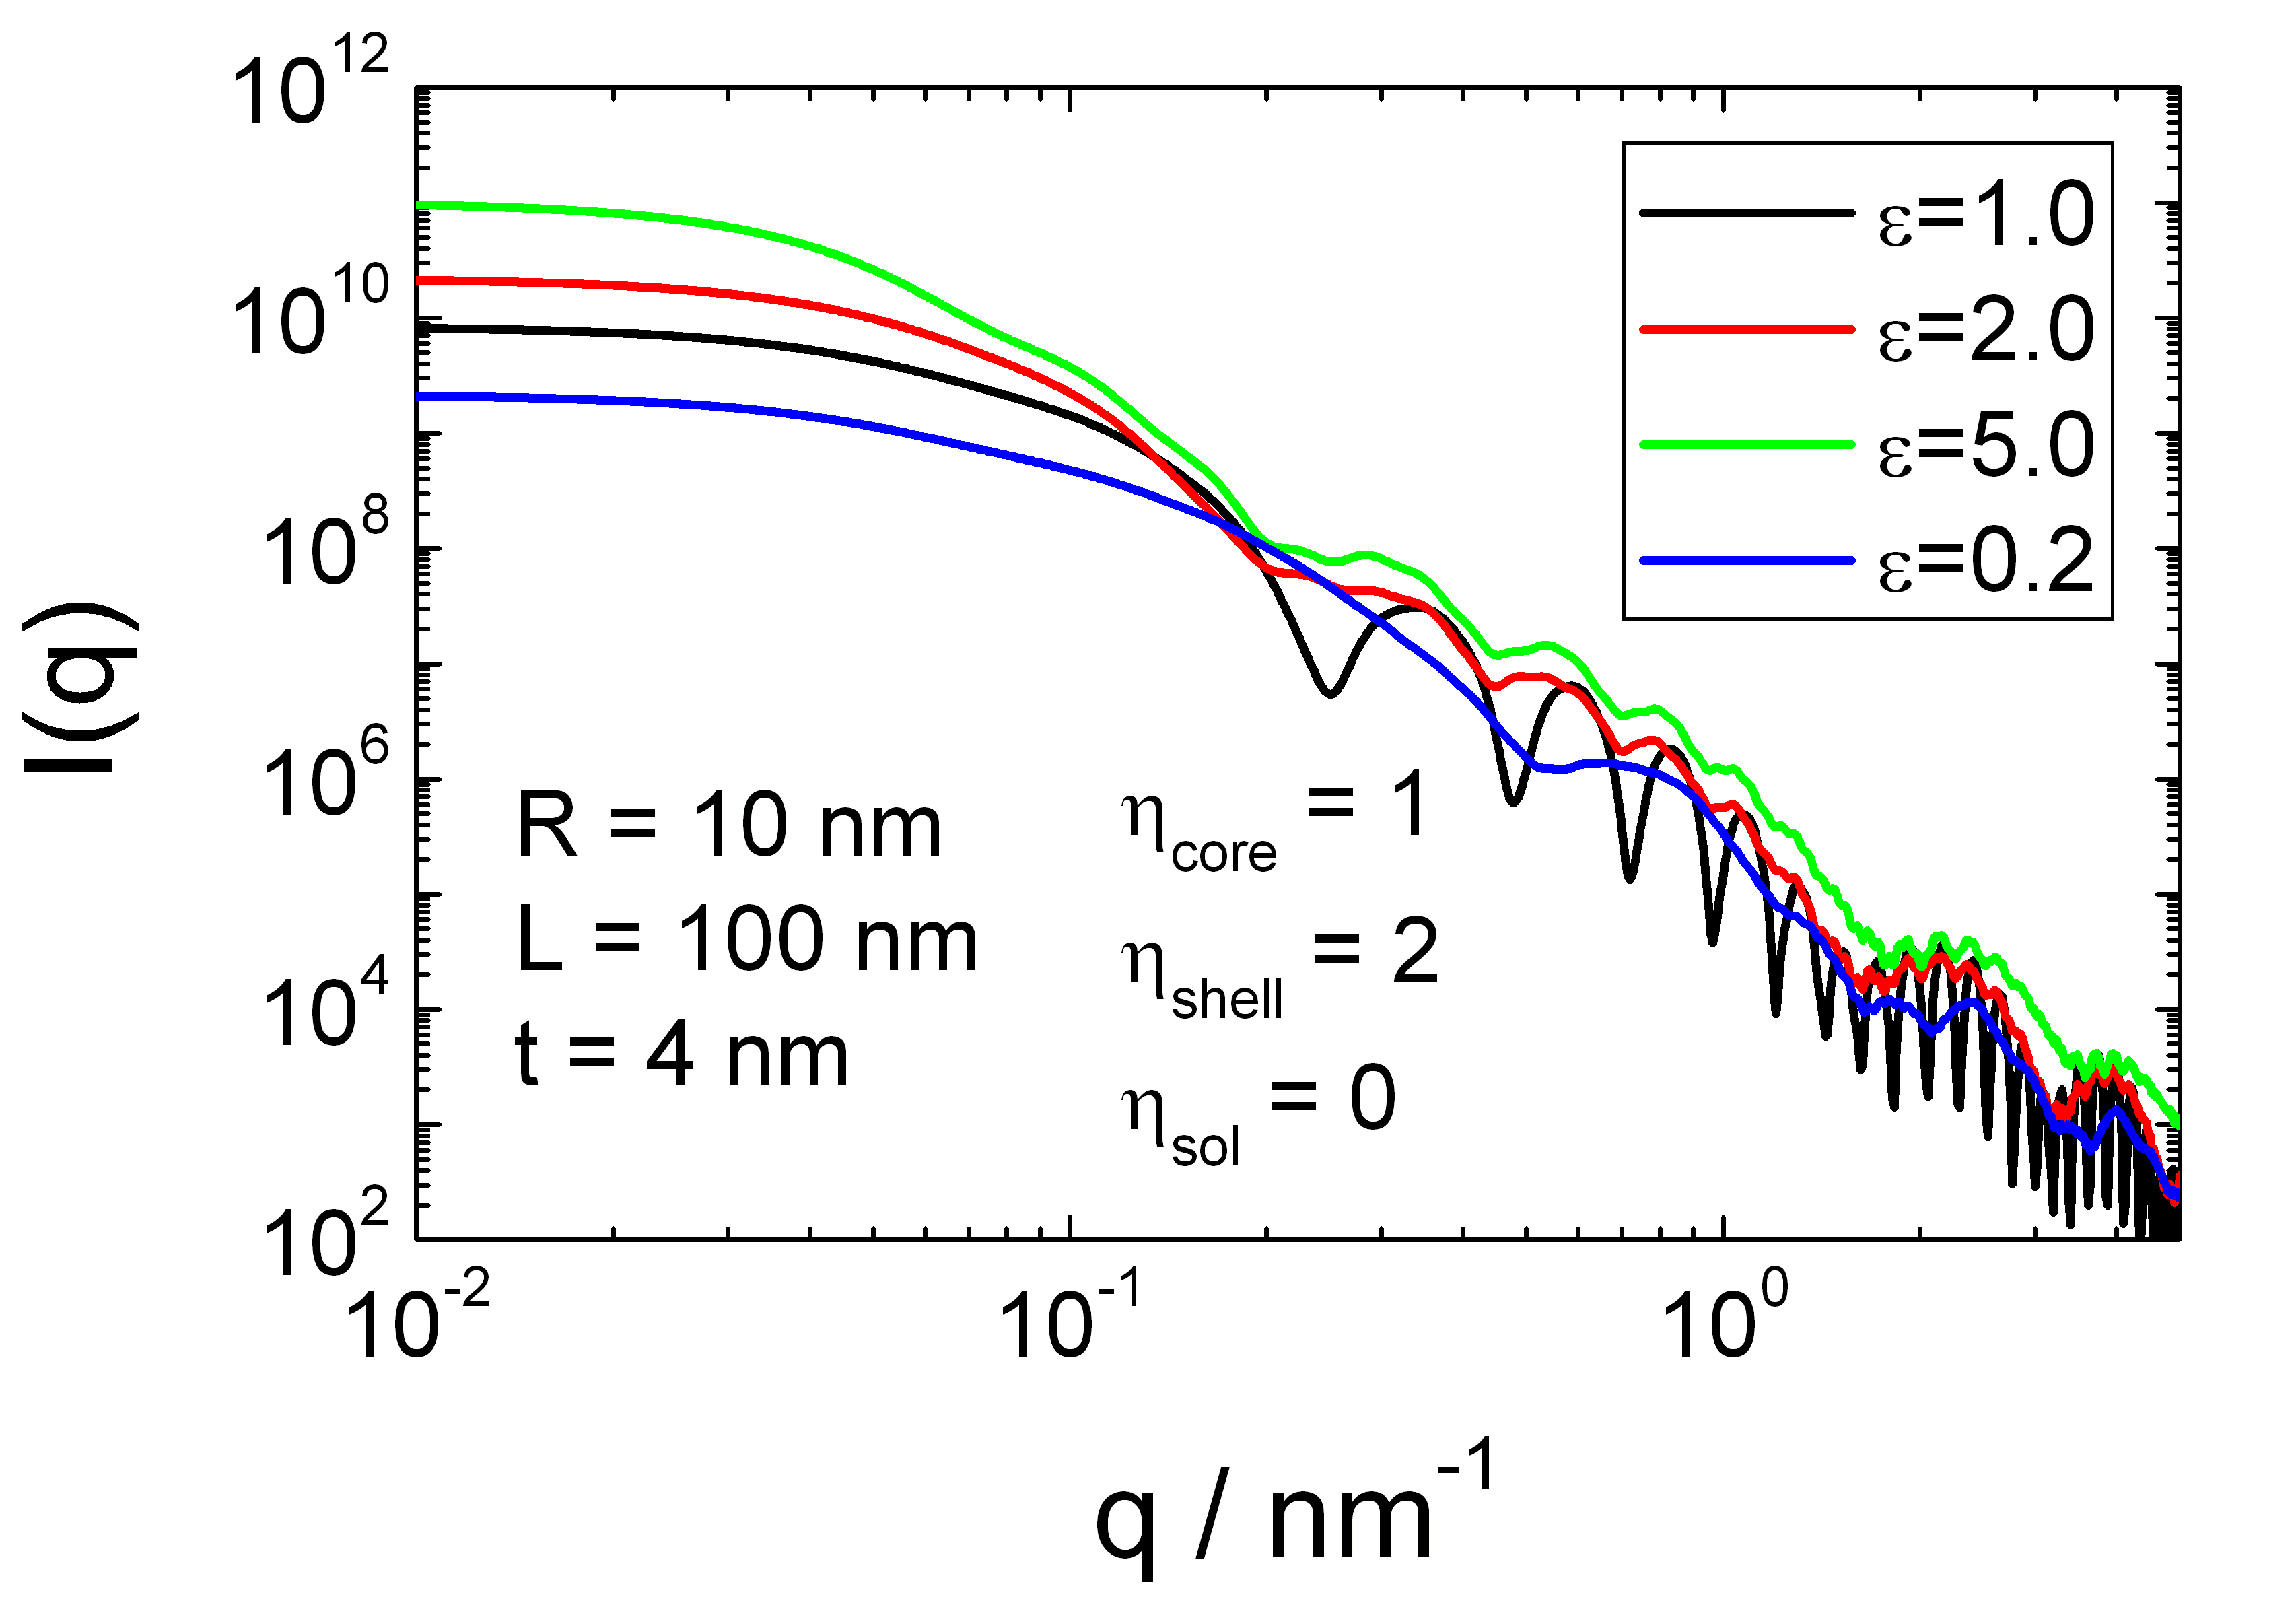
\includegraphics[width=0.65\textwidth]{../images/form_factor/cylindrical_obj/ellCylShell1.png}
\end{center}
\caption{Scattering intensity of a cylinder with elliptical cross-section.}
\label{fig:ellCylShell1}
\end{figure}

\begin{figure}[htb]
\begin{center}
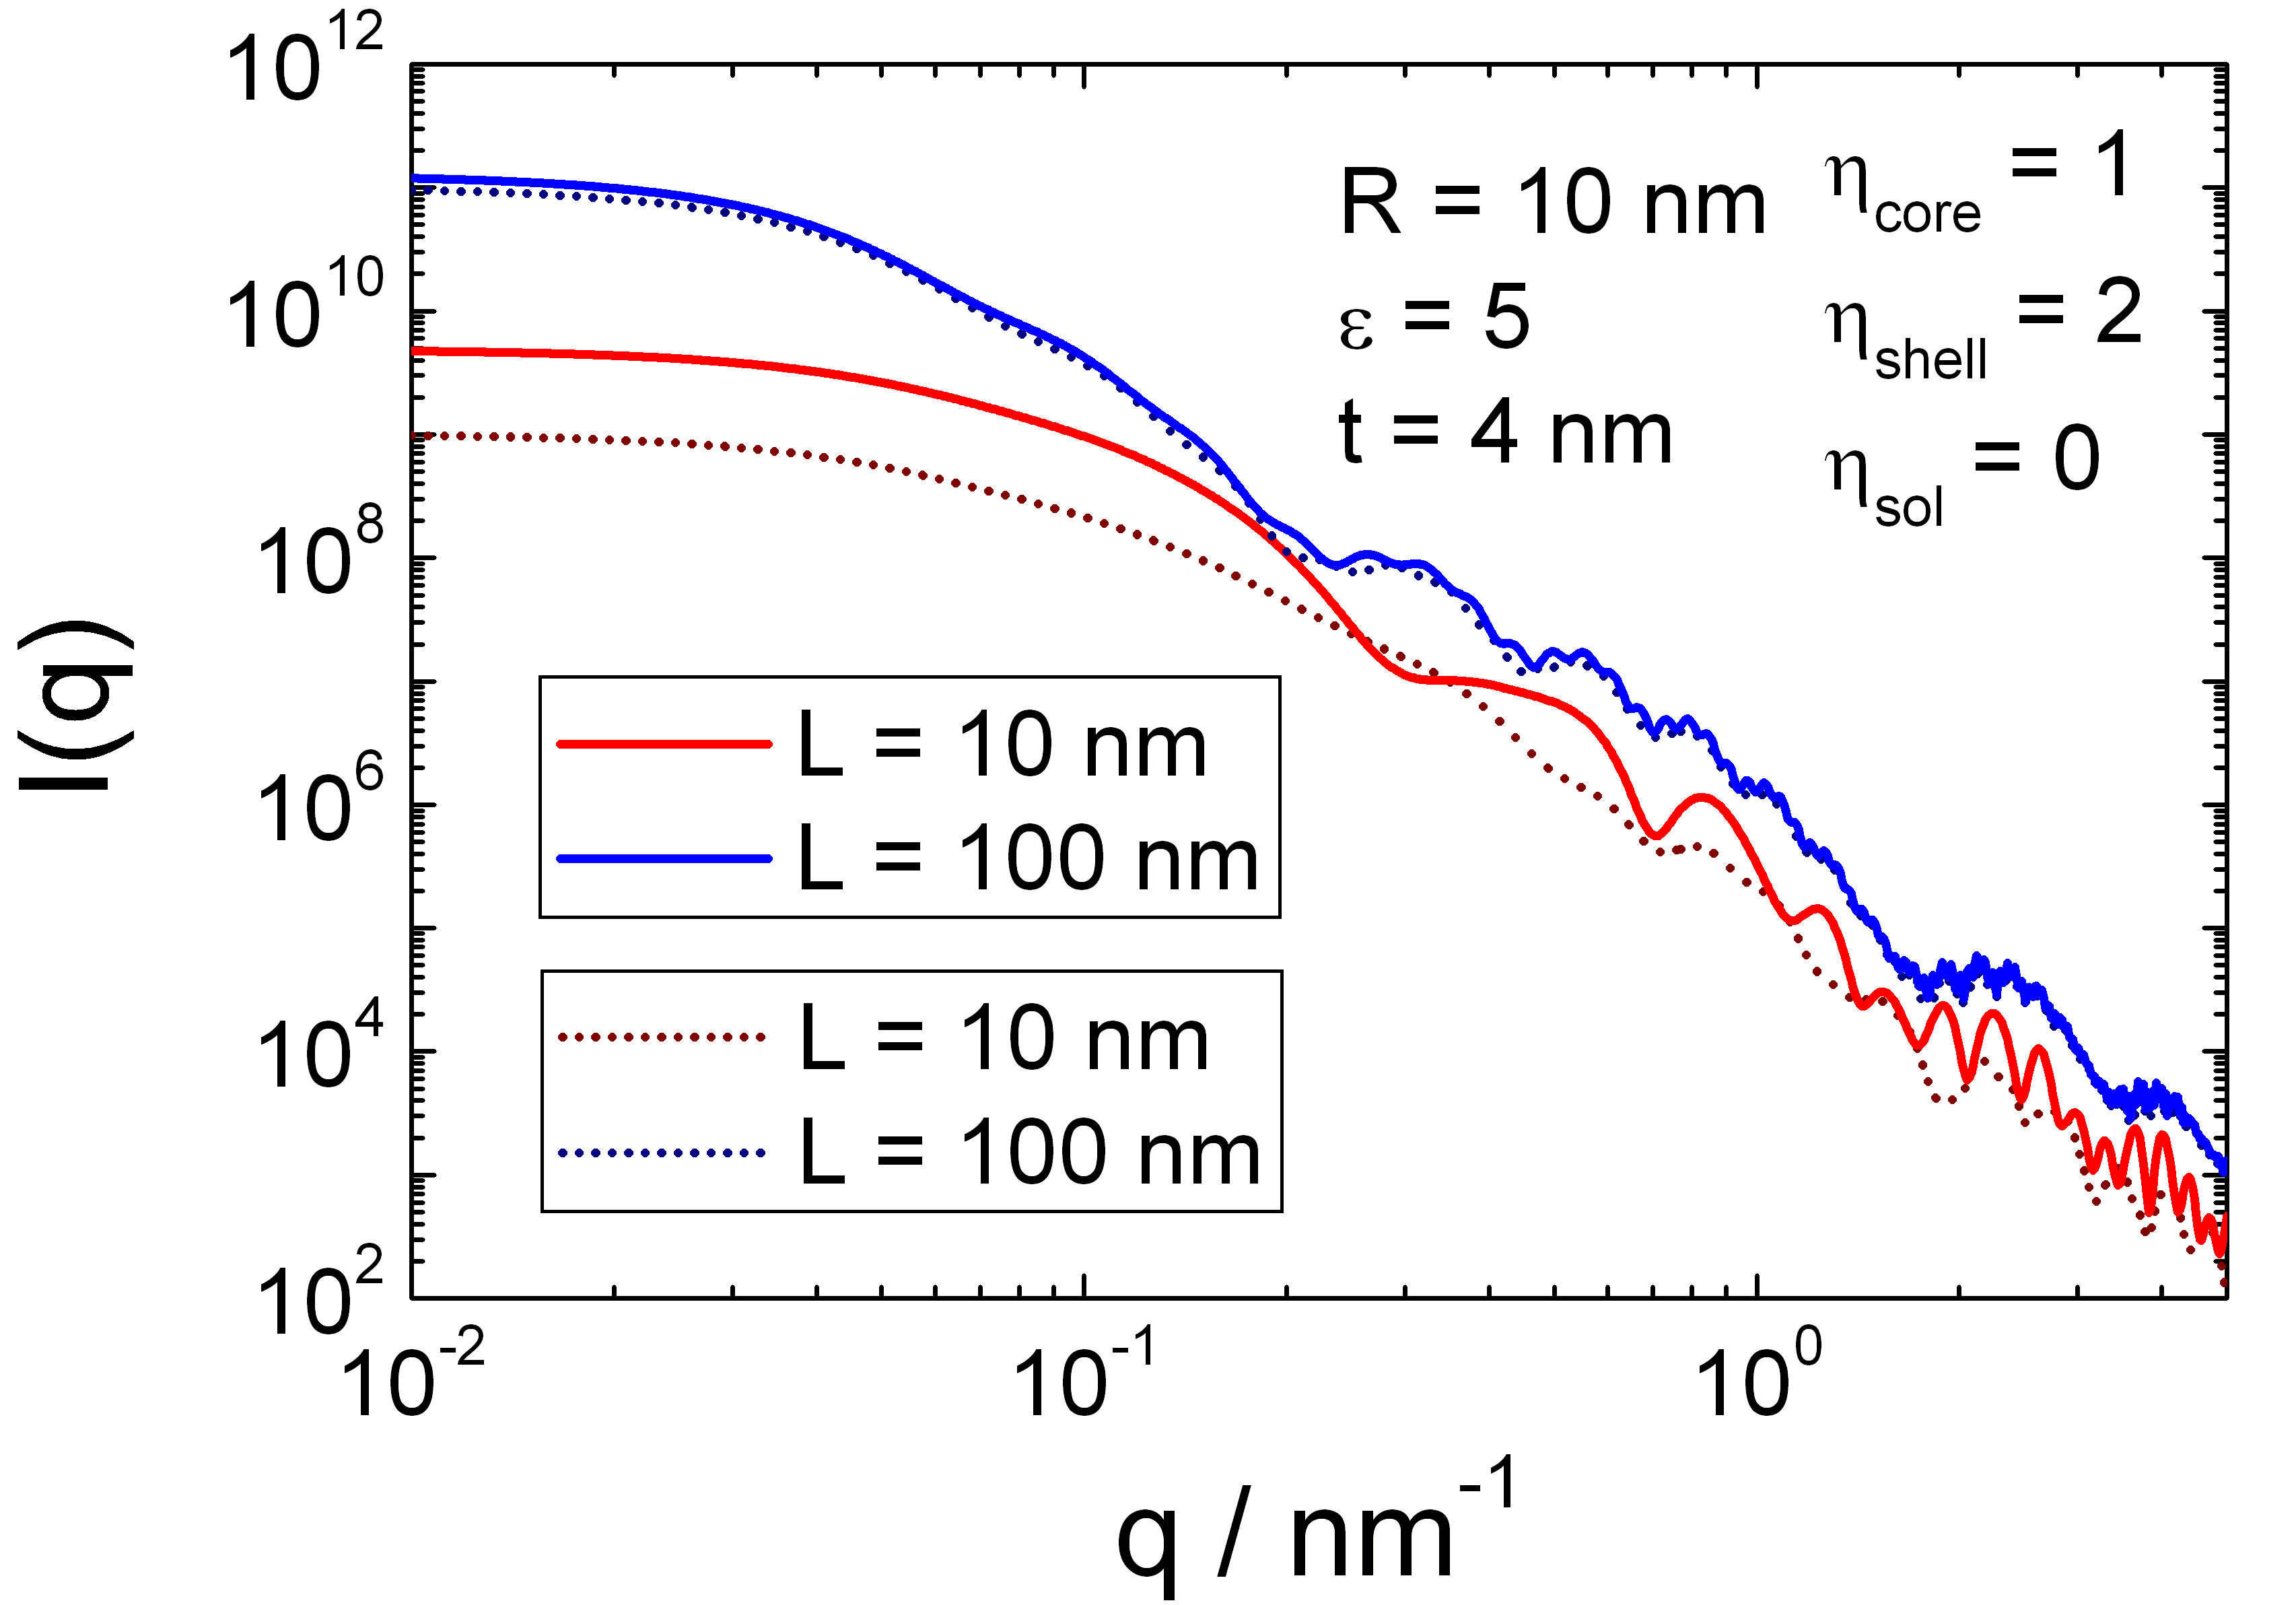
\includegraphics[width=0.65\textwidth]{../images/form_factor/cylindrical_obj/ellCylShell1_2.png}
\end{center}
\caption{Scattering intensity of a cylinder with elliptical cross-section with and without capped flat ends.}
\label{fig:ellCylShell1_2}
\end{figure}

\vspace{5mm}

\noindent For very long cylinders a faster approximation for the
uncapped version can be used \texttt{Pcs:ellCylSh}
combined with the structure factor \texttt{P'(Q):Rod}.
The implemented approximation is the following
\begin{align}
  I_\text{Long\_ellCylShell}(q) = & P'(q) P_\text{cs}(q) \\
  P'(q)  = & 2 \frac{\text{Si}(q L)}{qL} - \left(\frac{\sin(qL/2)}{qL/2}\right) \\
  \text{Si}(x) & = \int_0^x\!\frac{\sin t}{t}\,\,dt \\
  r(R,\epsilon,t,\phi) &= \sqrt{(R+t)^2\sin^2(\phi)+(\epsilon R+t)^2\cos^2(\phi)}\\
  P_\text{cs}(q)  =  \frac{2}{\pi} \int_0^{\frac{\pi}{2}}& \biggl(
            \frac{2J_1(qr(R,\epsilon,0,\phi))}{qr(R,\epsilon,0,\phi)}
            \left(\eta_\text{core}-\eta_\text{shell}\right)\epsilon R^2L\pi + \label{eq:PcsEllCylSh}\\
         &
            \frac{2J_1(q(r(R,\epsilon,t,\phi))}{qr(R,\epsilon,t,\phi)}
            \left(\eta_\text{shell}-\eta_\text{sol}\right)(R+t)(\epsilon R+t)L\pi
      \biggr)^2  \, d\phi \nonumber
\end{align}

\hspace{1pt}\\
\uline{Input Parameters for model \texttt{Pcs:ellCylSh}:}\\
\begin{description}
\item[\texttt{R}] core radius $R$
\item[\texttt{epsilon}] stretching factor $\epsilon$ of cross-section
\item[\texttt{t}] shell thickness $t$
\item[\texttt{eta\_core}] scattering length density $\eta_\text{core}$ of cylinder core
\item[\texttt{eta\_shell}] scattering length density $\eta_\text{shell}$ of cylinder shell
\item[\texttt{eta\_sol}] scattering length density $\eta_\text{sol}$ of solvent
\end{description}

\begin{figure}[htb]
\begin{center}
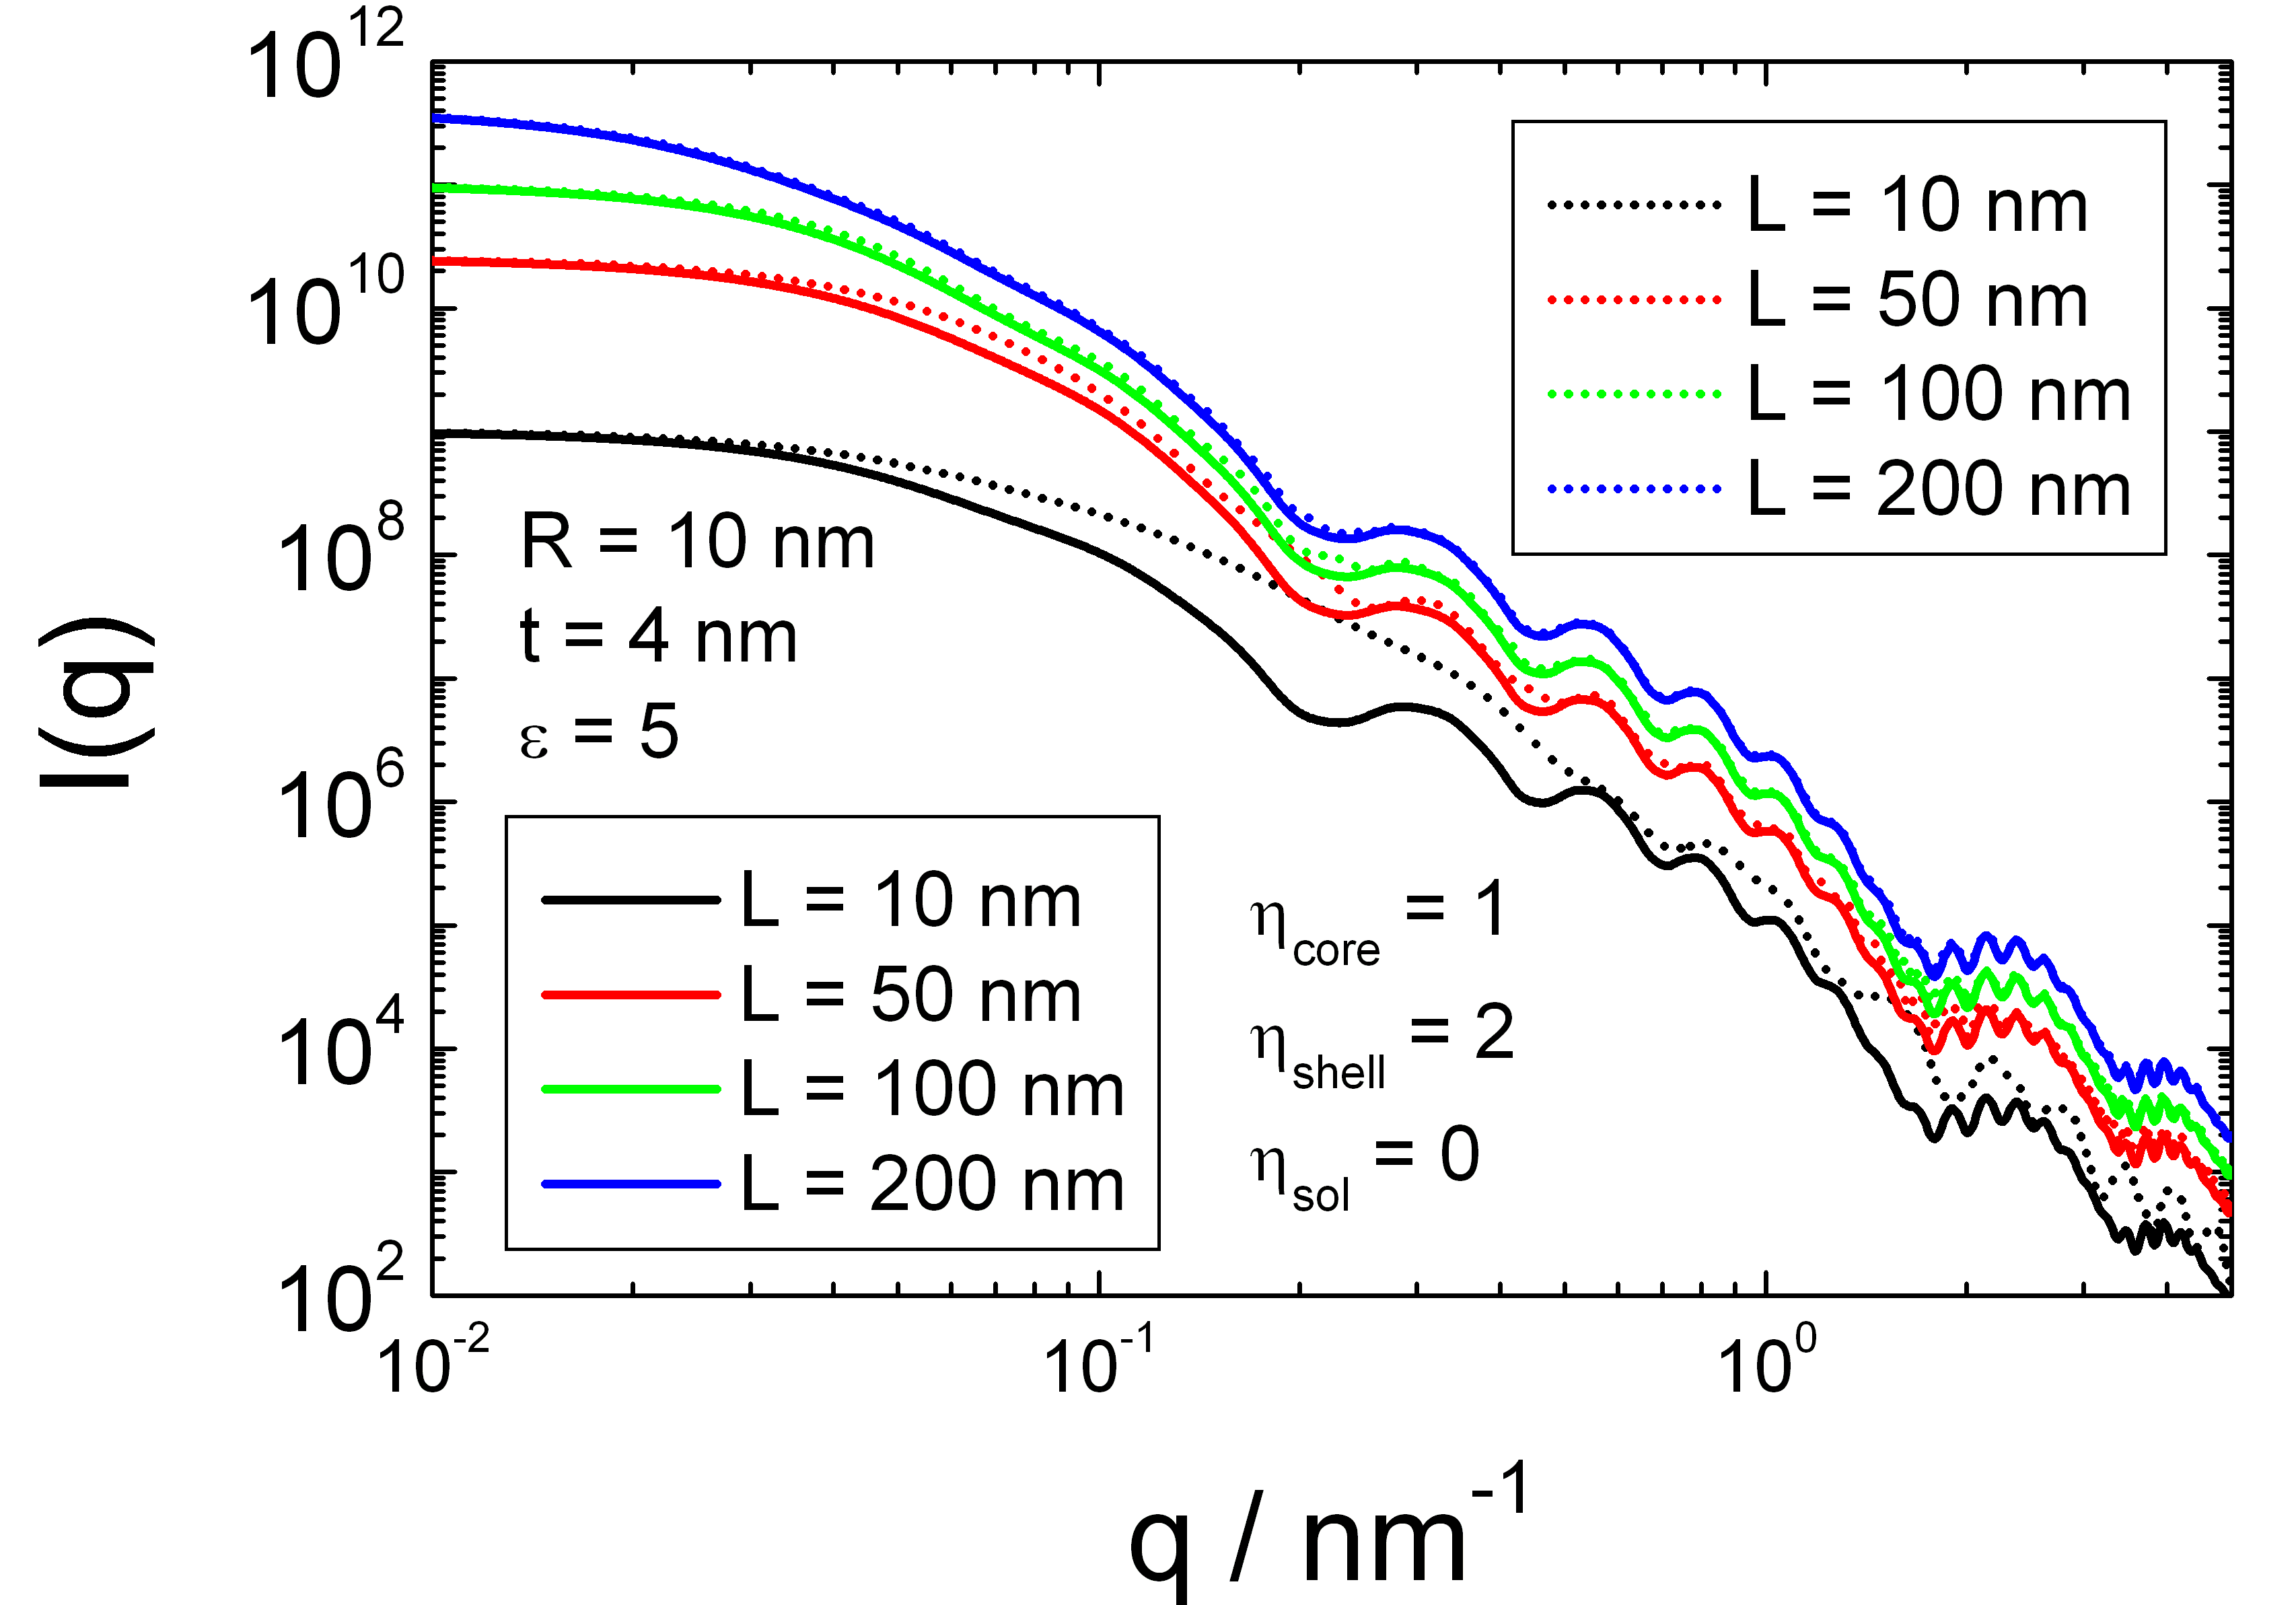
\includegraphics[width=0.65\textwidth]{../images/form_factor/cylindrical_obj/Pcs_ellCylShell.png}
\end{center}
\caption{Scattering intensity of a cylinder with elliptical cross-section.
The exact solutions \texttt{ellCylShell1} (dotted lines) are compared
with \texttt{Pcs:ellCylSh} (solid lines), which is only valid for very long cylinders $L \gg 2R$. }
\label{fig:Pcs_ellCylShell}
\end{figure}

%%%%%%%%%%%%%%%%%%%%%%%%%%%%%%%%%%%%%%%%%%%%%%%%%%%%%%%%%%%%%%%%%%%%%%%%%%%%%%%%%%%%%%%%%%%%

\clearpage
\subsection{Random oriented solid cylinder with circular cross-section and globular end caps}
\label{sect:capped_cylinder}
~\\

\begin{figure}[htb]
\begin{center}
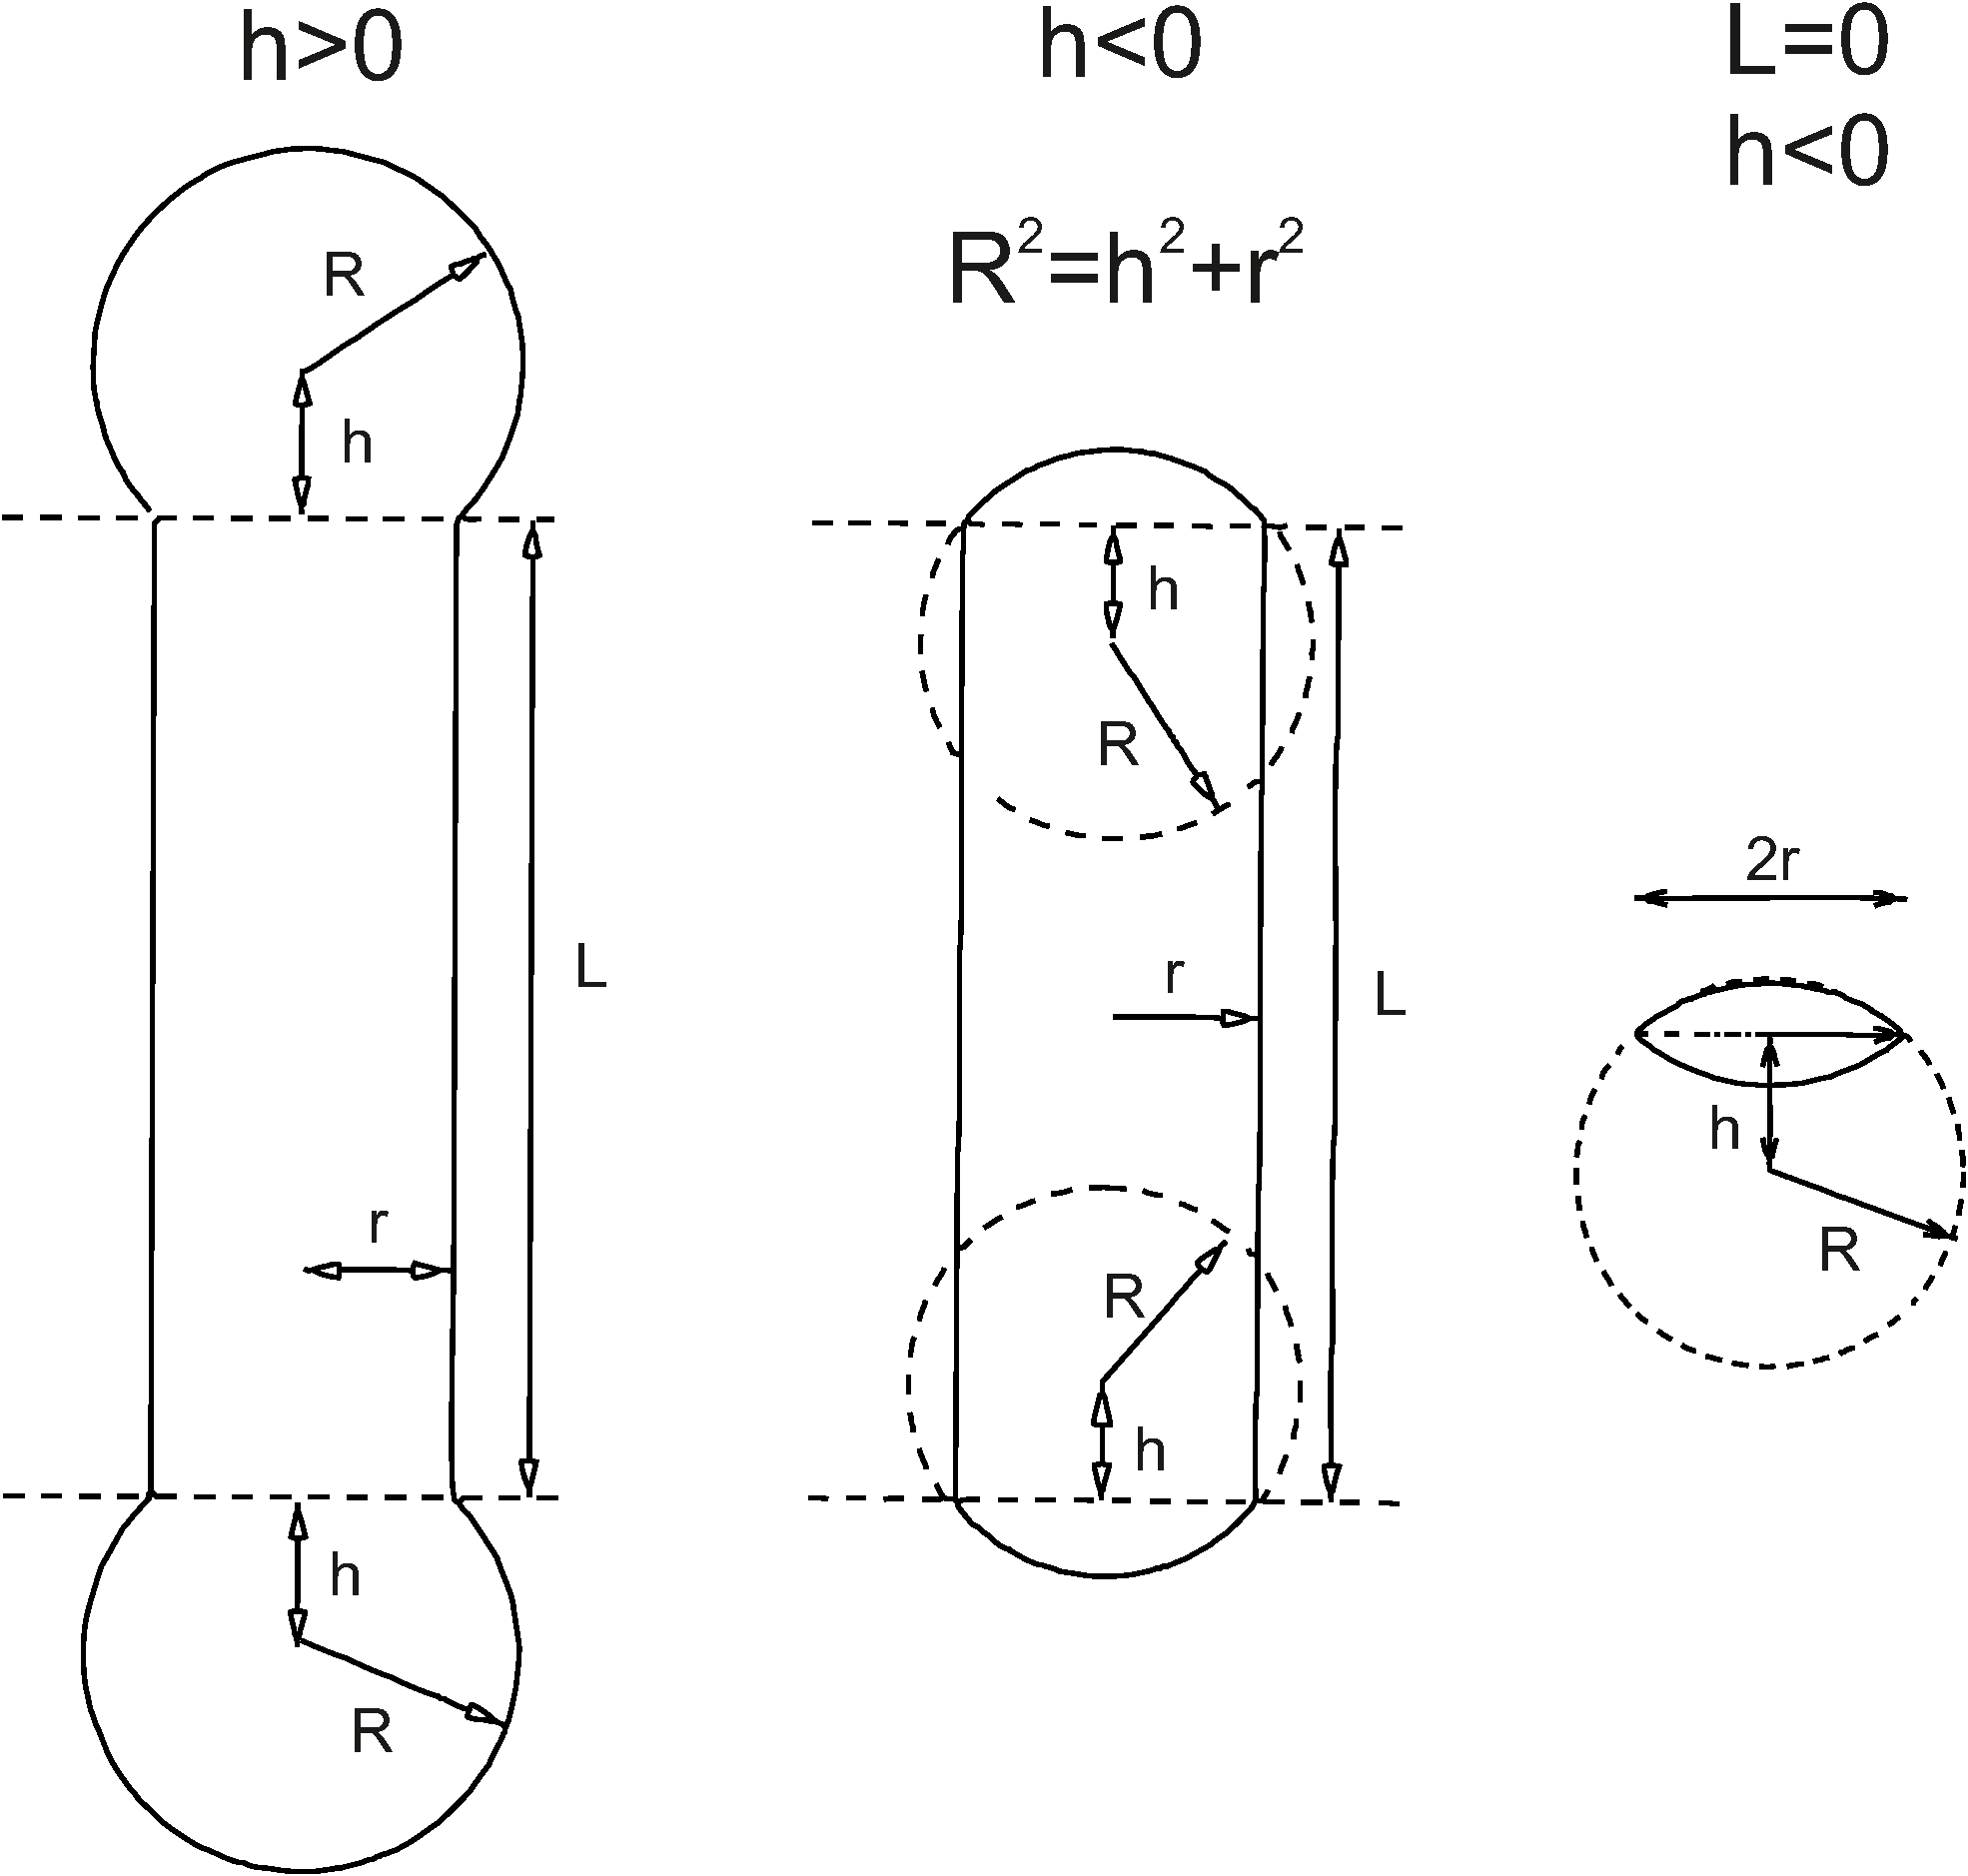
\includegraphics[width=0.75\textwidth]{../images/form_factor/cylindrical_obj/capped_cylinder.pdf}
\end{center}
\caption{solid cylinders with circular cross-section and globular end caps}
\label{fig:capped_cylinder}
\end{figure}

The scattering from cylinders with globular end caps have been studied by \cite{Kaya:aj5008,Kaya:aj5016}.
There form factor also contain the special case of hemispherical end-caps given by \cite{Cusack1981}. They obtain for the scattering amplitude the expression
\begin{align}\label{eq:CappedCylinders}
\begin{split}
  F(Q,r,L,h,\theta) &= \pi r^2 L \frac{QL/2 \cos(\theta)}{QL/2 \cos(\theta)} \frac{2\operatorname{J}_1(Qr\sin(\theta))}{Qr\sin(\theta)} \\
  & + 4\pi R^3 \int_{-h/R}^1 \mathrm{d}t \; \cos\left(Q(Rt+h+L/2)\cos(\theta)\right)\\
  & \times (1-t^2) \frac{\operatorname{J}_1\left(QR\sin(\theta)\sqrt{1-t^2}\right)}{QR\sin(\theta)\sqrt{1-t^2}}
\end{split}
\end{align}
Here $r$ is the radius of the cylinder, $R=\sqrt{h^2+r^2}$ the radius of the globular end caps, $h$ the offset of the globular end cap from the end of the cylinder and $L$ is the length of the cylinder. For $h>0$ the end caps are barbel like and for $h<0$ they are flat.

The scattering intensity of a random oriented cylinder with globular end caps reads as
\begin{align}\label{eq:randomoriented_cappedcylinders}
  I(Q) &= \int_0^{\pi/2} \abs{F(Q,r,L,h,\theta)}^2 \sin\theta \; \mathrm{d}\theta
\end{align}

\hspace{1pt}\\
\uline{Input Parameters for model \texttt{capped\_cylinder}:}\\
\begin{description}
\item[\texttt{r}] cylinder radius $r$
\item[\texttt{h}] center offset of cap from surface $h$. ($h<0$: flat end cap, $h>0$: barbel end caps)
\item[\texttt{L}] cylinder length $L$
\item[\texttt{eta}] scattering length density $\eta$ of cylinder
\end{description}

\noindent\uline{Note:}
\begin{itemize}
\item $r$ and $L$ are only physical for values larger than 0.
\item $h$ can be positive or negative depending on the direction of the offset.
\item the integration algorithm can be configured via GUI (via \texttt{integration strategy})
\end{itemize}

\begin{figure}[htb]
\begin{center}
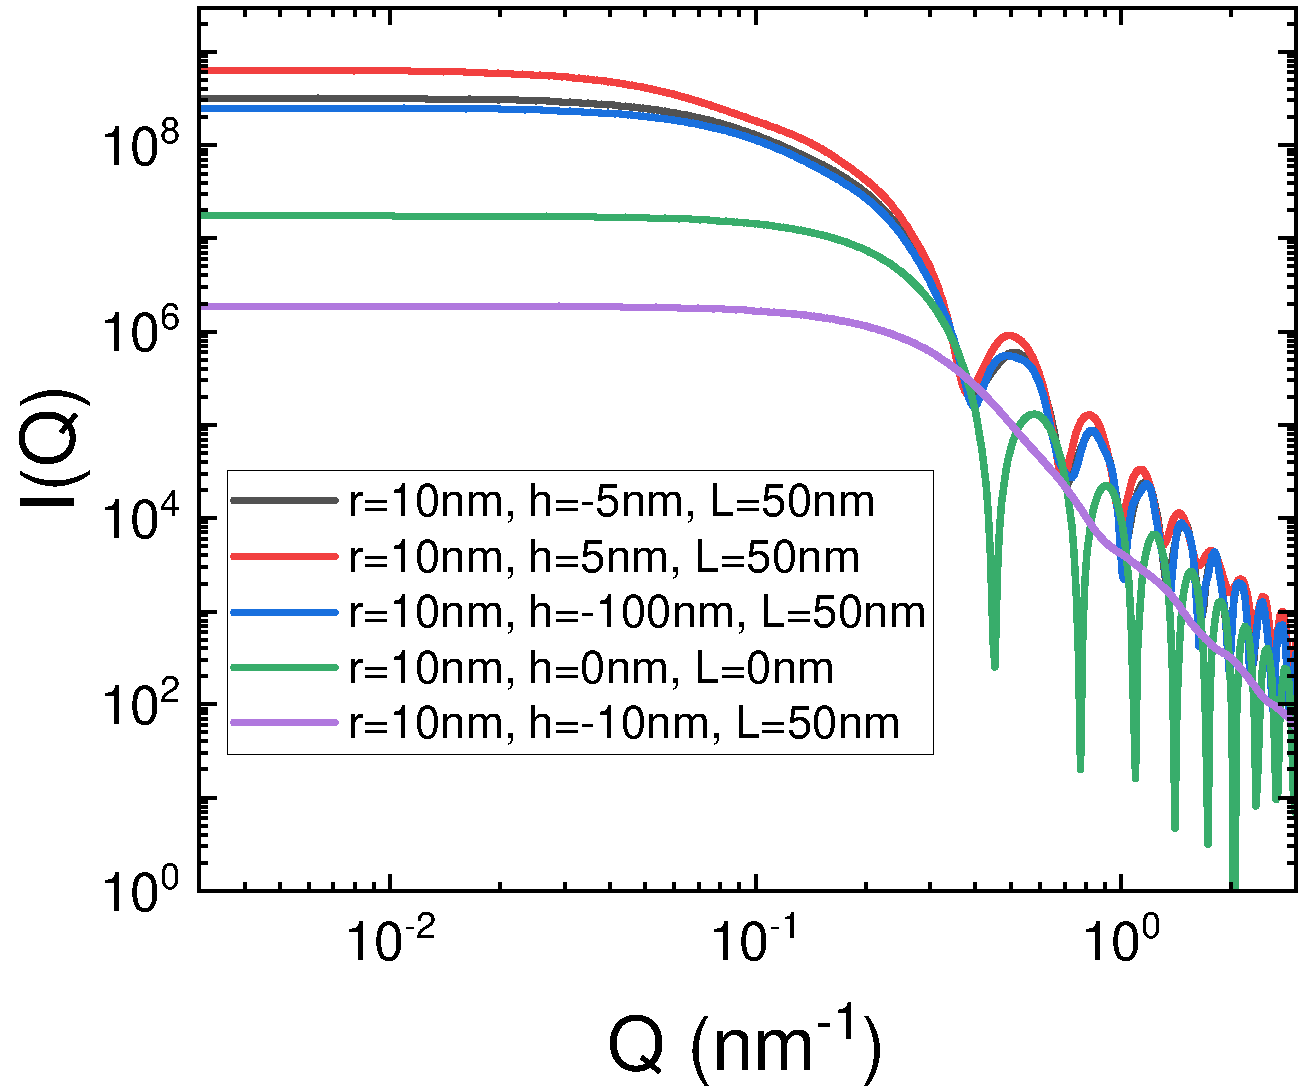
\includegraphics[width=0.75\textwidth]{../images/form_factor/cylindrical_obj/capped_cylinder_IQ.pdf}
\end{center}
\caption{scattering curves of random oriented capped cylinders with circular cross-section and globular end caps}
\label{fig:capped_cylinder_IQ}
\end{figure}

%%%%%%%%%%%%%%%%%%%%%%%%%%%%%%%%%%%%%%%%%%%%%%%%%%%%%%%%%%%%%%%%%%%%%%%%%%%%%%%%%%%%%%%%%%%%
\clearpage

\subsection{Cylinders packed in a hexagonal lattice with paracrystalline distortion}
\label{sect:CylHex_paracrystalline}
\hspace{1pt}\\
\begin{figure}[htb]
\begin{center}
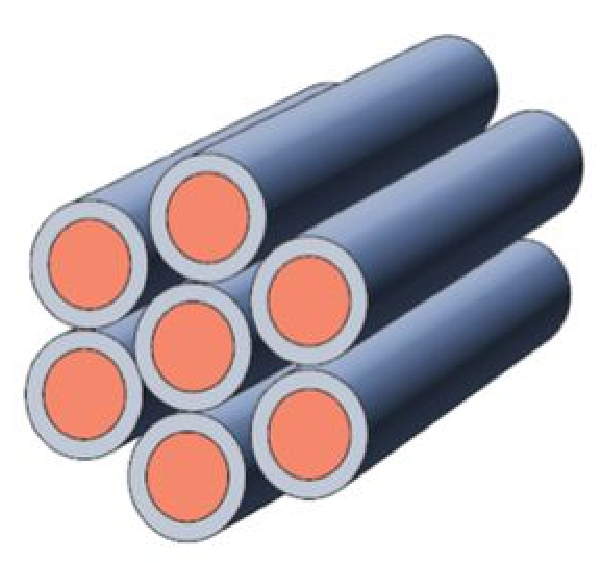
\includegraphics[width=0.5\textwidth]{../images/form_factor/cylindrical_obj/HEXcyl.pdf}
\end{center}
\caption{hexagonal packed long cylinders}
\label{fig:hex_long_cylinder}
\end{figure}
Hashimoto has given in \cite{Hashimoto1994} an analytical expression for hexagonal packed infinite long cylinders with a paracrystalline disorder. In a first case the scattering perpendicular to the cylinder axis is derived but also the random oriented case is given, where simply a Lorentz factor of $q^{-1}$ needs to be multiplied \cite{Shibayama1989,Glatter1982}.
In principle the two cases can be considered as the case of very thin rod-like structures as discussed in \ref{sec:very_anisotropic_particles}. For such thin random orientated particles the form factor can be factorized  in a cross-section term $P_\text{cs}(Q)$ for the shorter or thin dimension and a shape factor $P'(Q)$ for the long dimension.
\begin{align}
\label{eq:PprimePcs}
I(Q) &=P'(Q) P_{cs}(Q).
\end{align}
The cross section term for cylinder-symmetric structures is the zero order Hankel transform of the radial scattering length density profile $\eta(\rho)$
\begin{align}\label{eq:PcsHankel}
  P_{cs}(Q) & \abs{\int_0^\infty \eta(\rho) \rho\operatorname{J}_0(Q\rho)}^2
\end{align}
The cross-section term alone describes the scattering perpendicular to the cylinder axes and has to be used if the cylinder axis is perfectly aligned to the beam direction, i.e.\ perpendicular to the scattering vector, as e.g.\ done in \cite{Penttilae2019} to analyse textured wood samples.
In \cite{Hashimoto1994,Penttilae2019} the cross section term $P_{cs}(Q)$ is named $P_{cs}=I_\mathrm{cyl}(Q)$. The given model assumes, that also for the aligned cases only the cylinder axis are aligned to the beam axis but otherwise random orientations around that axis is assumed.
\begin{subequations}
\begin{align}
  I_\mathrm{cyl}(Q) &= \frac{1}{2\pi}\int_0^\infty I_\perp(Q,\psi) \mathrm{d}\psi \label{eq:paracystalHEXcylperp} \\
  I_\perp(Q,\psi) &= \langle \abs{F_\mathrm{cs}(Q)^2}\rangle + \abs{\langle F_\mathrm{cs}(Q)\rangle}^2 \left(S(Q)-1\right)\\
  F_\mathrm{cs}(Q,R) &= \int_0^\infty \eta(\rho) \rho\operatorname{J}_0(Q\rho) \mathrm{d}\rho = \pi R^2 \frac{\operatorname{J}_1(Qr)}{QR} \\
  S(Q) &= Z_1 Z_2  \\
  Z_k &= \frac{1-\abs{F_k}^2}{1-2\abs{F_k}\cos\left(\mathbf{Q}\mathbf{a}_k\right) + \abs{F_k}^2}  \label{eq:paraHEXZkvers_1} \\
  F_k &= \exp\left( -\frac12 \left(\frac{\Delta a}{a}\right)^2\left[\left(\mathbf{Q}\mathbf{a}_1\right)^2 + \left(\mathbf{Q}\mathbf{a}_2\right)^2\right]\right) \\
  \mathbf{Q}\mathbf{a}_1 &= -aQ\cos\left(\psi-\pi/6\right)\\
  \mathbf{Q}\mathbf{a}_2 &=  aQ\sin\left(\psi\right)
\end{align}
\end{subequations}
The lattice constant $a$ is assumed to have a certain paracrystalline distortion quantified by $\Delta a$. The structure factor of the hexagonal lattice has been introduced using the decoupling approach \cite{Kotlarchyk1983}, which involves two averages $\langle \abs{F_\mathrm{cs}(Q)^2}\rangle$ and $\abs{\langle F_\mathrm{cs}(Q)\rangle}^2$ of the cross-section amplitude. In case of a Gaussian distribution (see \ref{sec:GaussSD}) of cylinder radii with $\overline{R}$ being the maximum of the Gaussian distribution and $\Delta R=\sigma$ the width parameter according to eq.\ \ref{eq:GaussDistribution} so that
\begin{align}
\langle F_\mathrm{cs}(Q)\rangle &= \int_0^\infty \text{Gauss}(R,1,\Delta R,\overline{R}) F_\mathrm{cs}(Q,R) \mathrm{d}R \\
\langle F_\mathrm{cs}^2(Q)\rangle &= \int_0^\infty \text{Gauss}(R,1,\Delta R,\overline{R}) F_\mathrm{cs}^2(Q,R) \mathrm{d}R
\end{align}
To suppress the upturn in the structure factor at small $Q$-values a modification of the lattice factor $Z_k$  has been suggested in \cite{Penttilae2019} by approximating the lattice factor by
\begin{align}\label{eq:modifiedZk}
  Z_k &=
  \begin{cases}
        Z_k(Q_0), & 	\text{if $Q \leq  Q_0$}  \\
        Z_k(Q) 	, & 	\text{if $Q >     Q_0$}
  \end{cases} \\
  Q_0 &= 7.061\times 10^{-5} a^2 - 0.007413a + 0.2465
\end{align}
The polynominal dependencies of $Q_0$ has been determined in \cite{Penttilae2019}, where they found, that it is also almost independent on $\Delta a$.

~\\
\subsubsection{Scattering perpendicular to paracrystalline hexagonal packed cylinders} ~\\

For the scattering of the hexagonal packed cylinders perpendicular to the cylinder axes the intensity is given by eq.\ \ref{eq:paracystalHEXcylperp}. If the correction of the lattice factor in eq.\ \ref{eq:modifiedZk} is used or not can be set via a flag parameter. If \texttt{vers}$\le0$ the corrected lattice factor is used otherwise the original one in eq.\ \ref{eq:paraHEXZkvers_1}.

\begin{figure}[htb]
\begin{center}
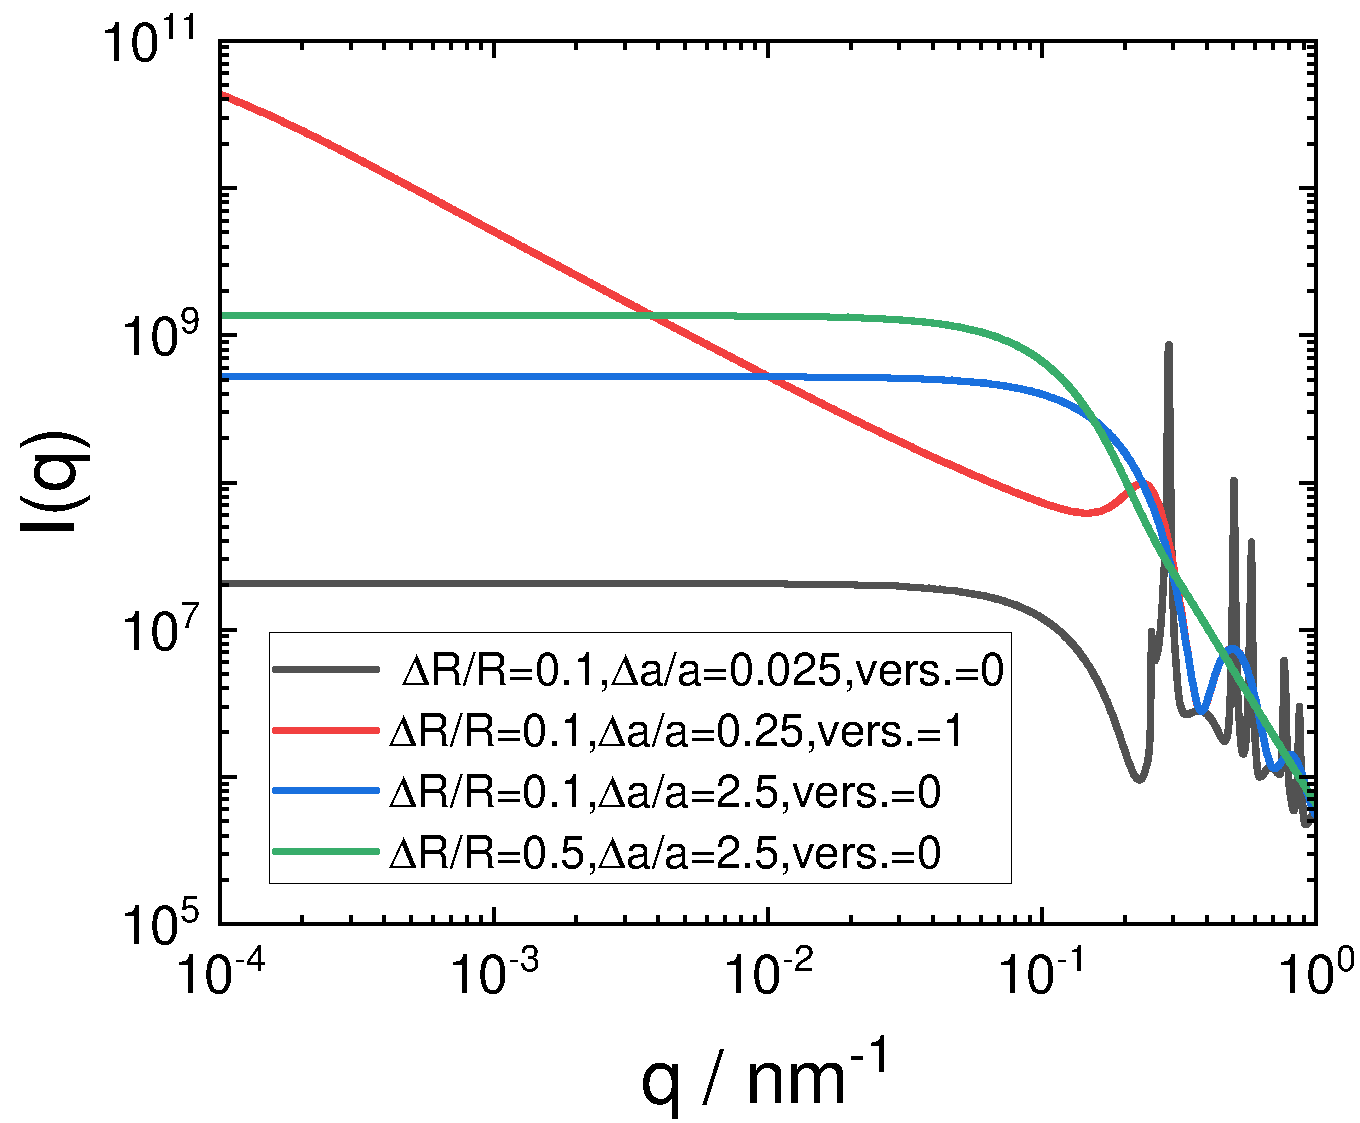
\includegraphics[width=0.75\textwidth]{../images/form_factor/cylindrical_obj/paracrystHEXcyl_perp.pdf}
\end{center}
\caption{Scattering intensity perpendicular to paracrystalline hexagonal packed cylinders.}
\label{fig:paracrystHEXcyl_perpIQ}
\end{figure}

\hspace{1pt}\\
\uline{Input Parameters for model \texttt{paracryst\_hex\_cyl\_perp}:}\\
\begin{description}
\item[\texttt{R}] avg.\ cylinder radius $R$
\item[\texttt{dR\_ratio}] Gaussian width parameter $\Delta R$ divided by average radius $\Delta R/R$
\item[\texttt{dummy}] not used
\item[\texttt{dummy}] not used
\item[\texttt{a}] lattice parameter $a$
\item[\texttt{da\_ratio}] paracrystalline distortion parameter $\Delta a$ divided by lattice constant $\Delta a/a$
\item[\texttt{vers.}] flag how the structure factor is calculated
\end{description}

\noindent\uline{Note:}
\begin{itemize}
\item the integration algorithm can be configured via GUI (via \texttt{integration strategy})
\end{itemize}

~\\
\subsubsection{Scattering of randomly oriented bundles of paracrystalline hexagonal packed cylinders} ~\\

The random oriented version of the previous form factor is in principle also able to probe the length of the cylinders. The form factor is given by eq.\ \ref{eq:PprimePcs} with the cross-section term of eq.\ \ref{eq:paracystalHEXcylperp} and $P'(Q)$ given by eq.\ \ref{eq:PprimeRod} describing the scattering of a thin rod with a LogNorm length distribution. As for the previous version a parameter is introduced to define if the correction of the lattice factor in eq.\ \ref{eq:modifiedZk} is used or not. The version  can be set via a flag parameter. If \texttt{vers}$\le0$ the corrected lattice factor is used otherwise the original one in eq.\ \ref{eq:paraHEXZkvers_1}.

\hspace{1pt}\\
\uline{Input Parameters for model \texttt{paracryst\_hex\_cyl\_rnd}:}\\
\begin{description}
\item[\texttt{R}] avg.\ cylinder radius $R$
\item[\texttt{dR\_ratio}] Gaussian width parameter $\Delta R$ divided by average radius $\Delta R/R$
\item[\texttt{dummy}] not used
\item[\texttt{dummy}] not used
\item[\texttt{a}] lattice parameter $a$
\item[\texttt{da\_ratio}] paracrystalline distortion parameter $\Delta a$ divided by lattice constant $\Delta a/a$
\item[\texttt{vers.}] flag how the structure factor is calculated
\item[\texttt{L}] mode of cylinder length distribution $L$
\item[\texttt{sigma\_L}] LogNorm width parameter for cylinder length $\sigma_\mathrm{L}$
\end{description}

\begin{figure}[htb]
\begin{center}
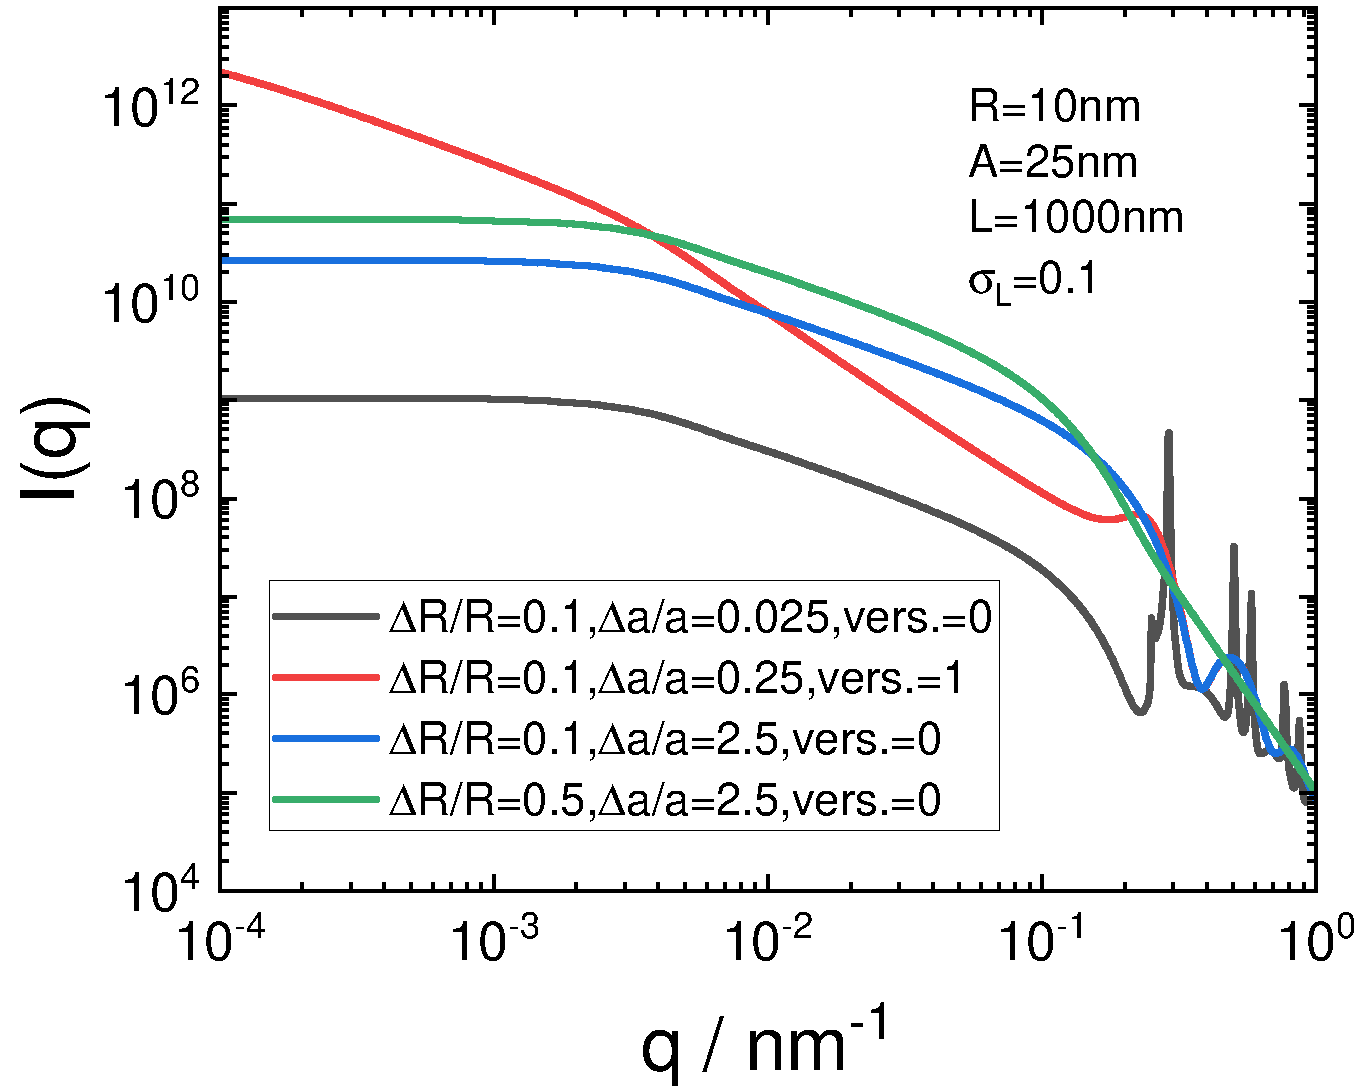
\includegraphics[width=0.75\textwidth]{../images/form_factor/cylindrical_obj/paracrystHEXcyl_rnd.pdf}
\end{center}
\caption{Scattering intensity randomly oriented bundles of paracrystalline hexagonal packed cylinders.}
\label{fig:paracrystHEXcyl_rndIQ}
\end{figure}

\noindent\uline{Note:}
\begin{itemize}
\item the integration algorithm can be configured via GUI (via \texttt{integration strategy})
\end{itemize}
%%%%%%%%%%%%%%%%%%%%%%%%%%%%%%%%%%%%%%%%%%%%%%%%%%%%%%%%%%%%%%%%%%%%%%%%%%%%%%%%%%%%%%%%%%%%
\clearpage

\subsection{Torus with elliptical shell cross-section}  \cite{Kawaguchi2001,Forster1999}
\label{sect:Torus}
\hspace{1pt}\\

\begin{figure}[htb]
\begin{center}
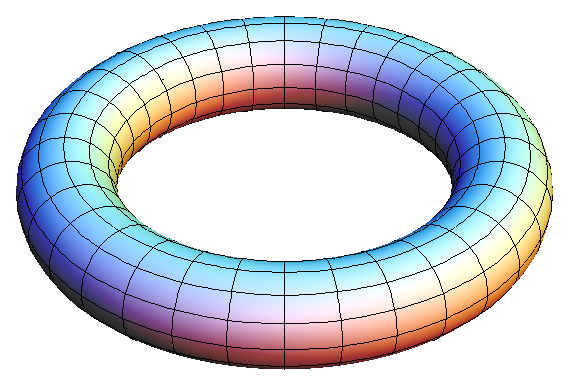
\includegraphics[width=0.575\textwidth]{torus.png}
\end{center}
\begin{center}
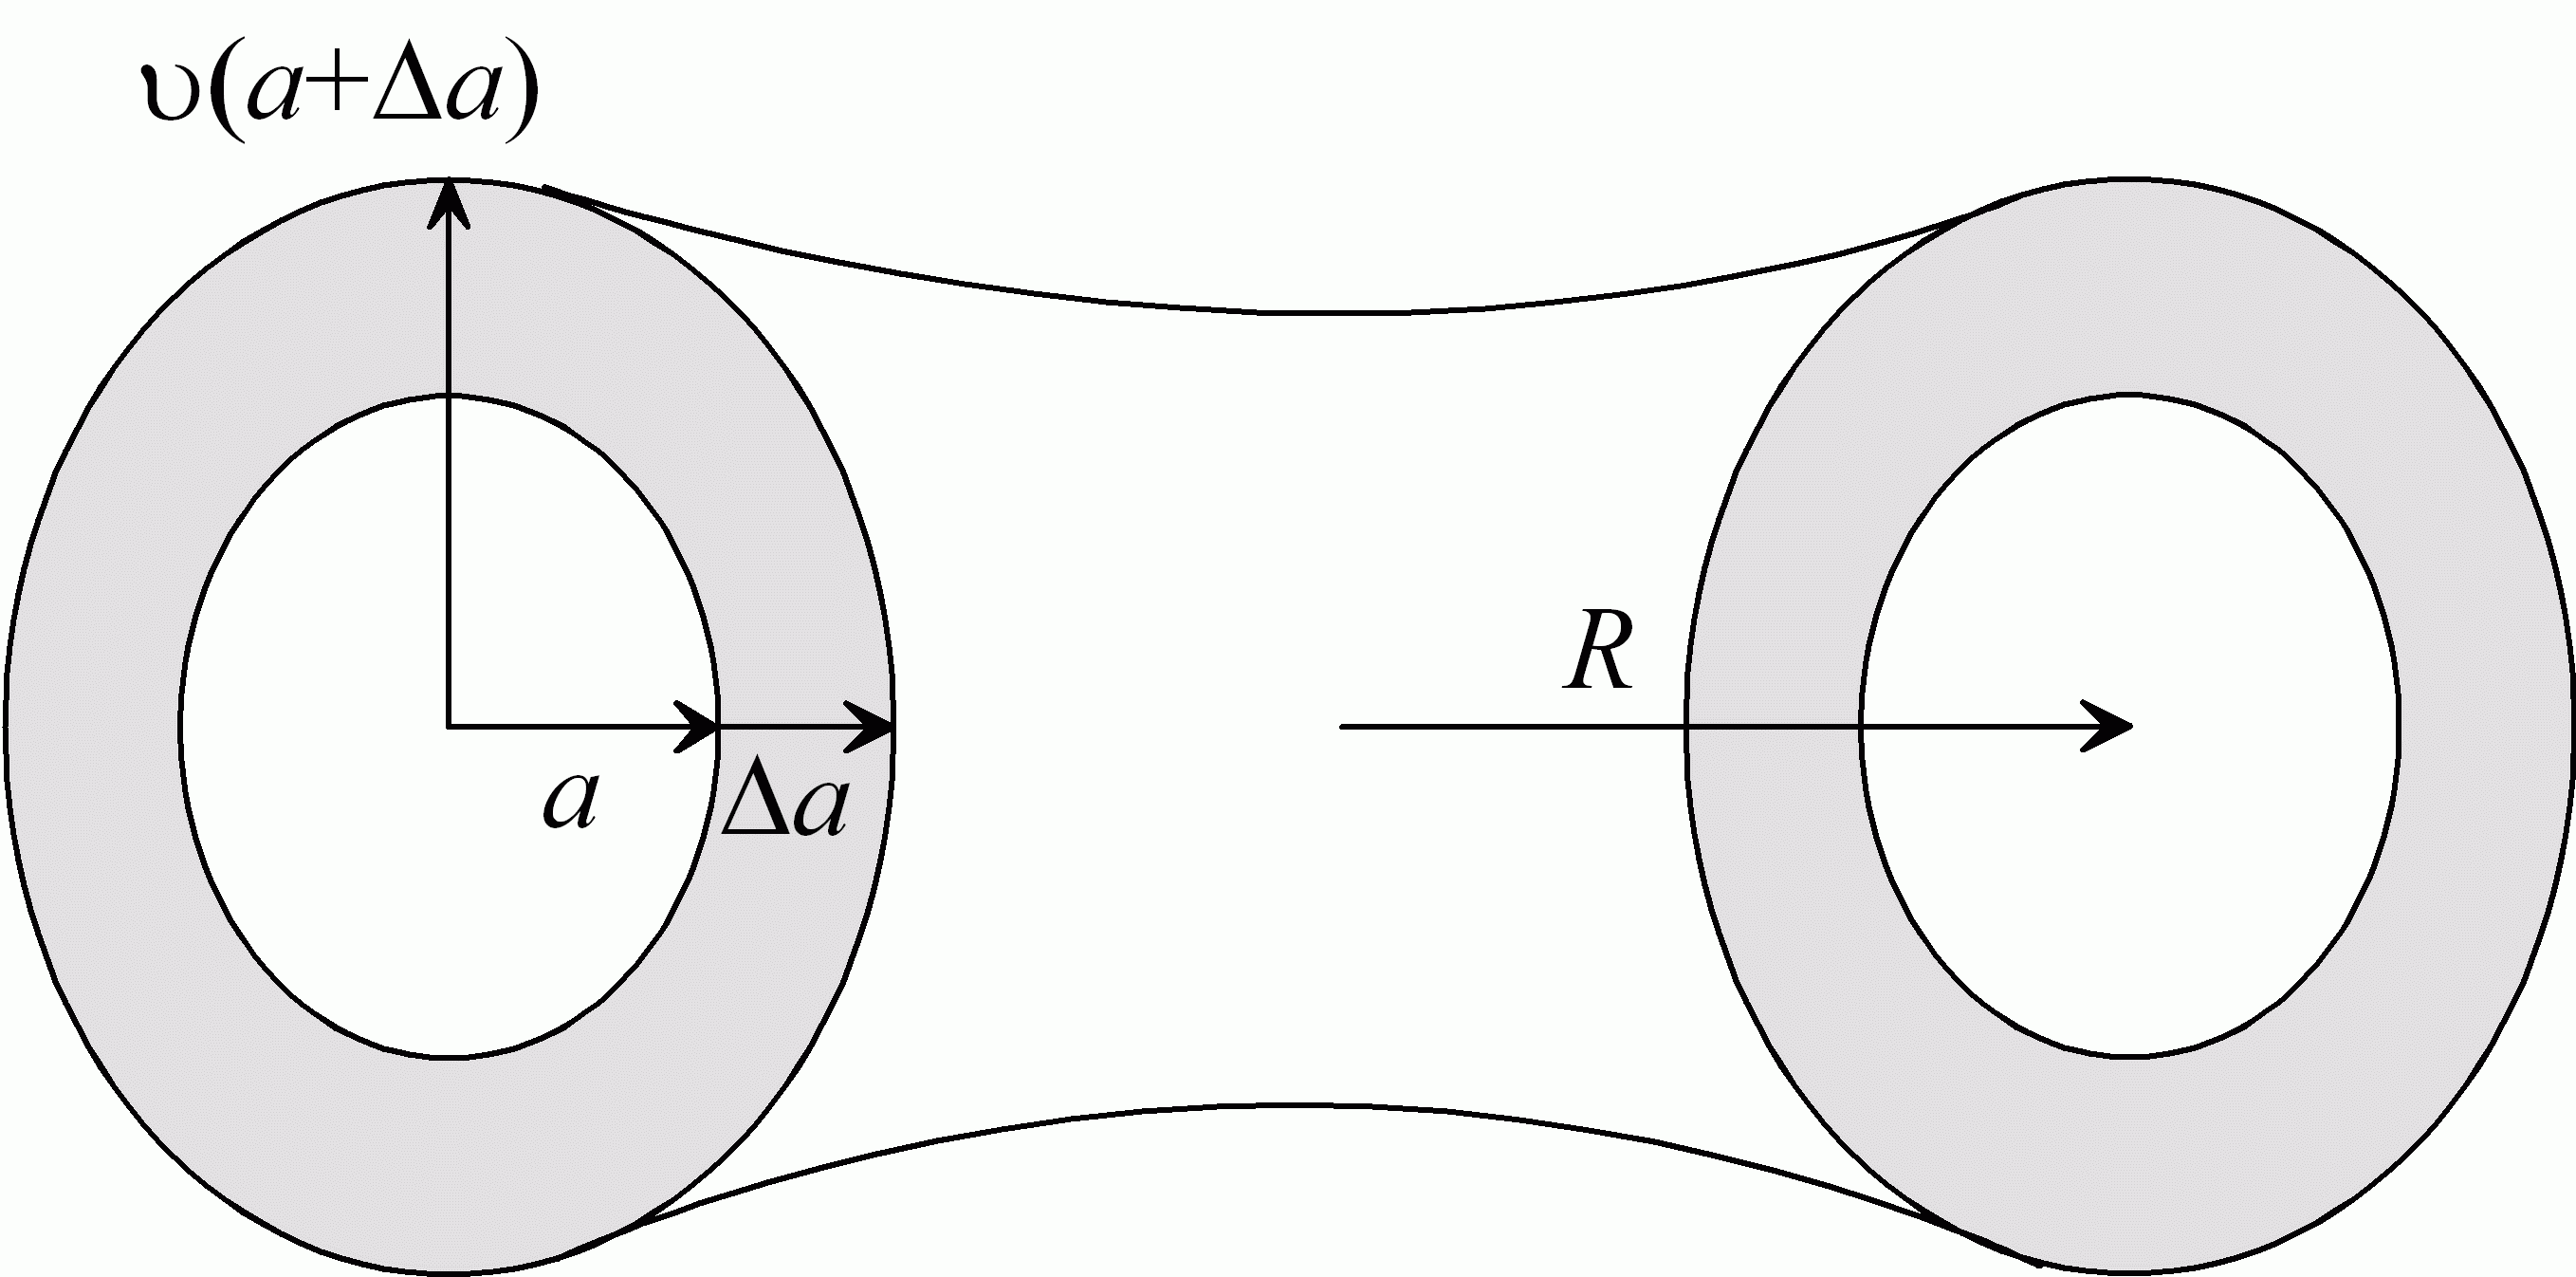
\includegraphics[width=0.6\textwidth]{torus_sh_xsect.png}
\end{center}
\caption{} \label{torus}
\end{figure}
\begin{align}
F_\text{torus}(Q,\Theta,R,x,\nu,\Delta\eta) & = \int_{\operatorname{max}\{0,R-x\}}^{R+x}
4\pi r \Delta\eta \frac{J_0(Qr\sin\Theta) \sin(
Q\gamma(r)\cos\Theta)}{Q\cos(\Theta)} \; dr \label{eq:torus1}
\end{align}
\begin{align}
\text{with } \gamma(r) &= \nu \sqrt{x^2-(r-R)^2}
\end{align}
\begin{align}
I_\text{torus}(Q,R,a,\nu,\Delta\eta) &= \int_0^{\pi/2}
\abs{F_\text{torus}(Q,\Theta,R,a,\nu,\Delta\eta)}^2 \sin\Theta  \;
d\Theta
\end{align}
\begin{align}
I_\text{torus,sh}(Q,R,a,\Delta a,\nu,\Delta\eta_{sh},\Delta\eta_c)
= \int_0^{\pi/2} \Bigl\lvert & F_\text{torus}(Q,\Theta,R,a+\Delta
a,\nu,\Delta\eta_{sh}) \\
-&F_\text{torus}(Q,\Theta,R,a,\nu,\Delta\eta_c)\Bigr\rvert^2
\sin\Theta  \;  d\Theta \nonumber
\end{align}
An alternative form factor for $F_\text{torus}$ following \cite{Forster1999} is
\begin{align}
F_\text{torus}(Q,\Theta,R,x,\nu,\Delta\eta)  = 2\pi\int_{-x}^{x}
\bigg[
 & R_{(+)} J_1(QR_{(+)}\sin\theta) \\
-& R_{(-)} J_1(QR_{(-)}\sin\theta) \bigg]
\frac{\cos(Qz\cos\theta)}{Q\sin\theta} \; dz \nonumber
\end{align}
with $R_{(\pm)} = R\pm\nu\sqrt{x^2-z^2}$

\hspace{1pt}\\
\uline{Input Parameters for model \texttt{torus}:}\\
\begin{description}
\item[\texttt{R}] distance between center of tube to center of torus $R$
\item[\texttt{a}] radius of tube core
\item[\texttt{Delta\_a}] shell thickness of tube shell $\Delta a$
\item[\texttt{nu}] stretching factor of elliptical torus cross-section $\nu$
\item[\texttt{eta\_c}] scattering length density of core $\eta_c$
\item[\texttt{eta\_sh}] scattering length density of shell $\eta_{sh}$
\item[\texttt{eta\_sol}] scattering length density of core $\eta_{sol}$
\end{description}

\noindent\uline{Note:}
\begin{itemize}
\item the integration algorithm can be configured via GUI (via \texttt{integration strategy})
\item for $R-a-\Delta a <0$ the integration in \ref{eq:torus1} starts at 0 as a lower limit. In the extreme case $R=0$ the form factor is the one of an elliptical shell.
\end{itemize}

\begin{figure}[htb]
\begin{center}
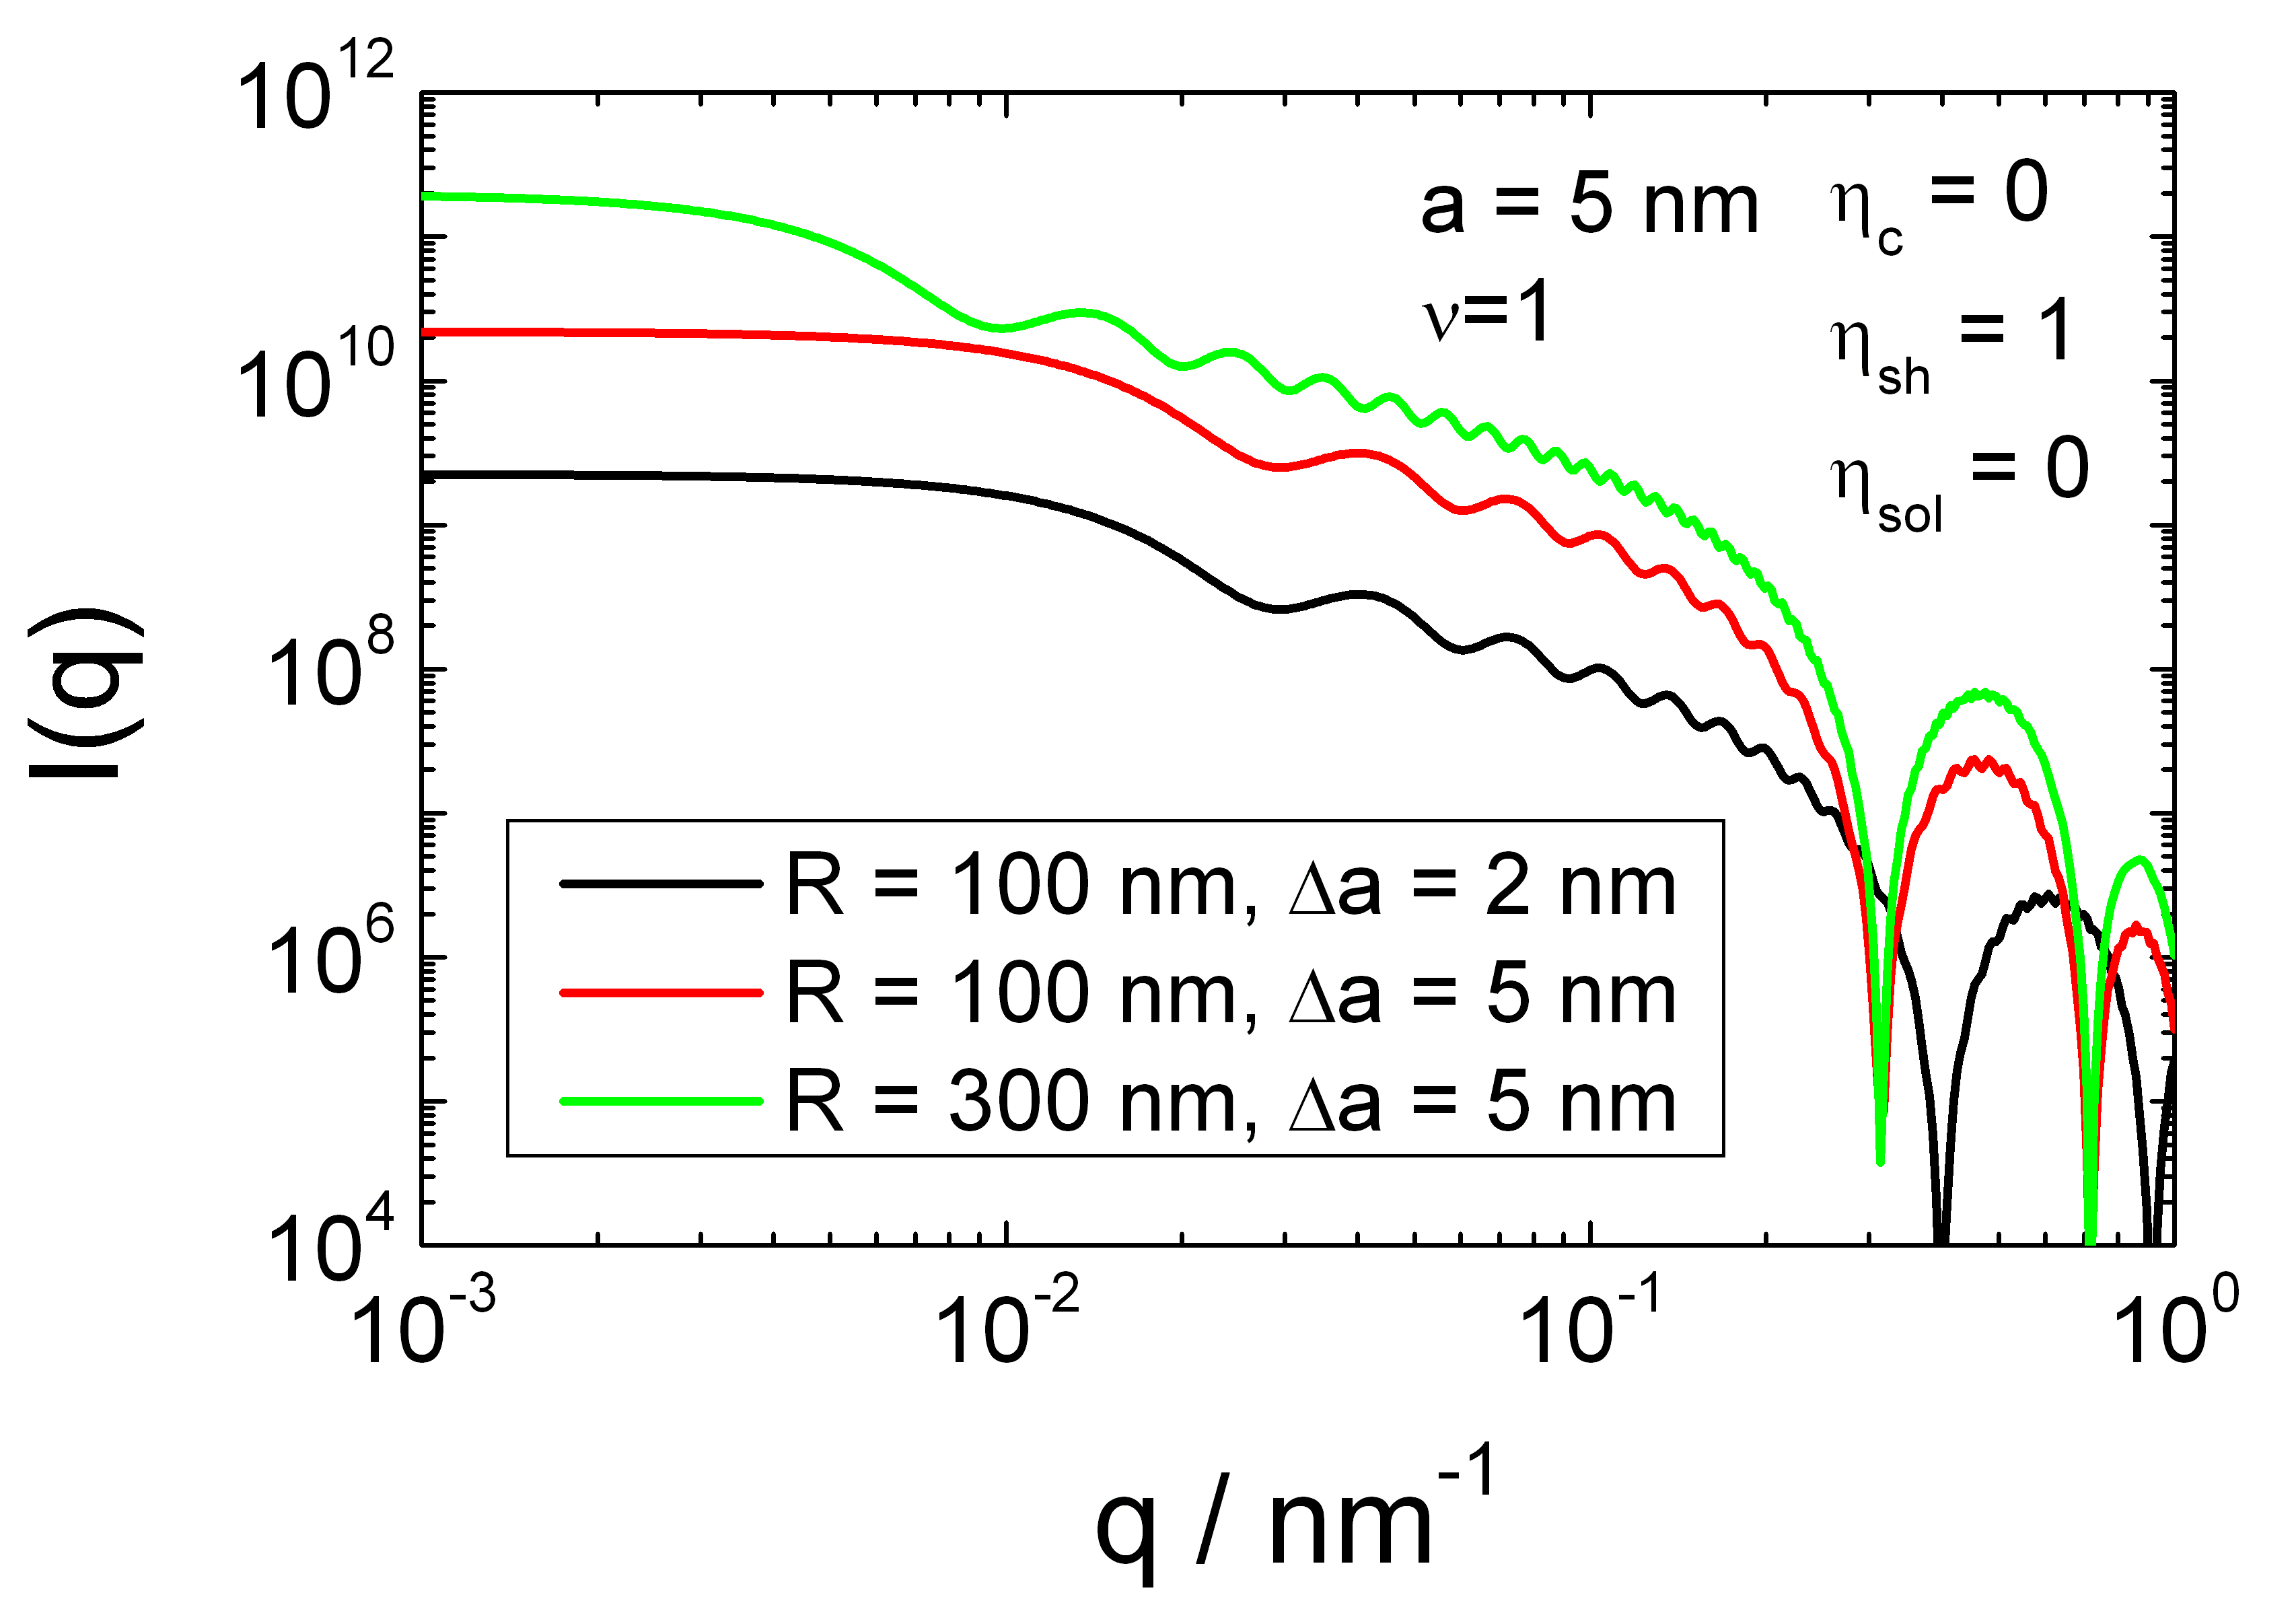
\includegraphics[width=0.75\textwidth]{../images/form_factor/cylindrical_obj/Torus.png}
\end{center}
\caption{Scattering intensity of a torus.}
\label{fig:Torus}
\end{figure}


%%%%%%%%%%%%%%%%%%%%%%%%%%%%%%%%%%%%%%%%%%%%%%%%%%%%%%%%%%%%%%%%%%%%%%

%\newpage
%\subsection{stacked tori with elliptical shell cross-section} ~\\
%\begin{figure}[htb]
%\begin{center}
%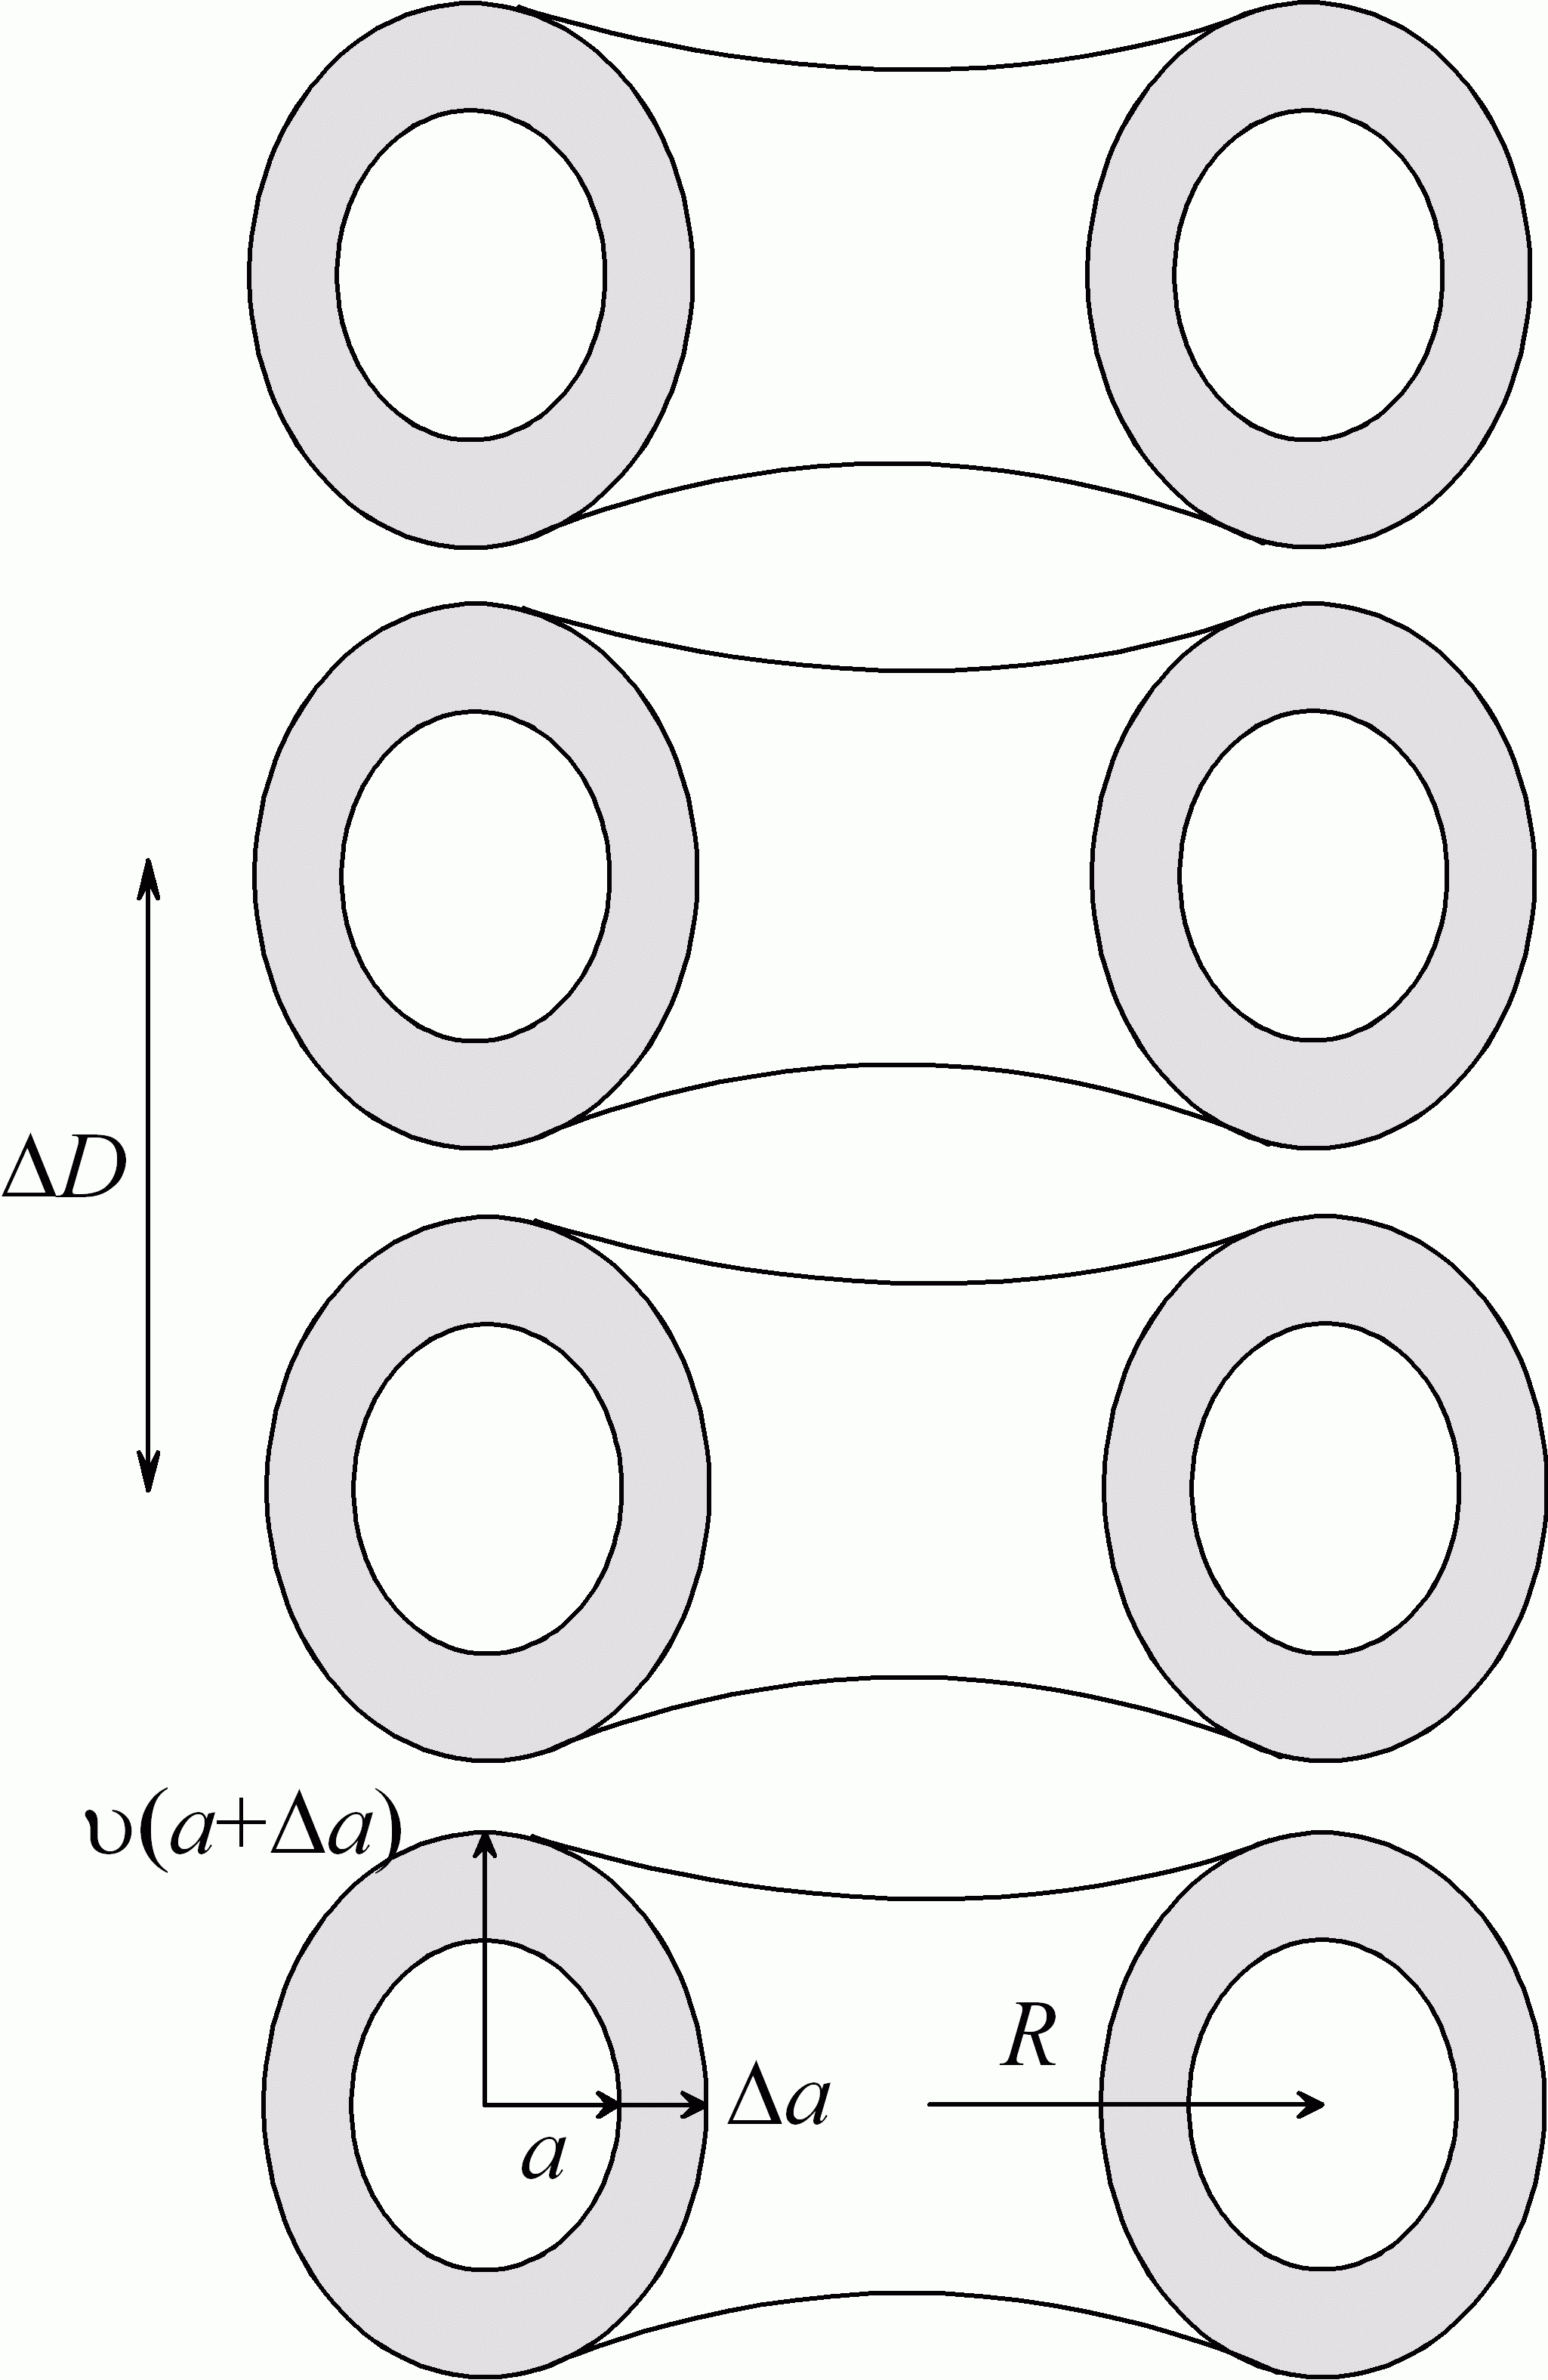
\includegraphics[width=0.55\textwidth,height=0.8\textwidth]{stacked_torus.png}
%\end{center}
%\caption{} \label{stackedTori}
%\end{figure}
%\begin{align}
%F_\text{stacked} & _\text{tori}(Q,\Theta,R,x,\nu,\Delta\eta,\Delta D,N)  =  \\
%& \sum_{n=1}^N \quad \int_{R-x}^{R+x} 4\pi r \Delta\eta
%\frac{J_0(Qr\sin\Theta) \sin(
%Q(\gamma(r)+\frac{2(n-1)-(N-1)}{4}\Delta
%D)\cos\Theta)}{Q\cos(\Theta)} \; dr \nonumber
%\end{align}
%The scattering intensity is than calculated in the same way as for
%a single torus with an elliptical shell cross-section.

%%%%%%%%%%%%%%%%%%%%%%%%%%%%%%%%%%%%%%%%%%%%%%%%%%%%%%%%%%%%%%%%%%%%%%%%%

\clearpage
\subsection{Helical structures} ~\\
Several approaches for describing the small angle scattering signal from randomly oriented helical structures have been published.
In \cite{Franklin1956,Puigjaner1974} a model of a double helix with a round cross section for each strand has been developed. For a fanlike cross section of a double helix a solution has been given by \cite{Schmidt1970,Pringle1971}. Fukuda et al.\ \cite{Fukuda2002} have extended the model to an arbitrary shaped cross section. In a model developed by Lebedev et al.\ \cite{Lebedev2003} it is assumed, that beads are arranged on a helical path assuming a single strand. In all models the helix is straight and its length dimension is large compared to all other characteristic length of the helix.
In \cite{Benham1980} a solution of a single helical strand which can have a secondary coiling has been described. In this paper the cross section of the helical strand is assumed to be infinitesimal thin.

~\\
\subsubsection{Fanlike helix} ~\\
Double helices with a fanlike cross section in the plane perpendicular to the helix axis have been described by by Schmidt and Pringle \cite{Schmidt1970,Pringle1971}. The model has been generalized by Fakuda et al.\ \cite{Fukuda2002} for an arbitrarily shaped cross section and by Teixeira et al.\ \cite{Teixeira2010} to a multi radial shell with fanlike cross section.
\begin{figure}[htb]
\begin{subfigure}[b]{.48\textwidth}
   \centering
   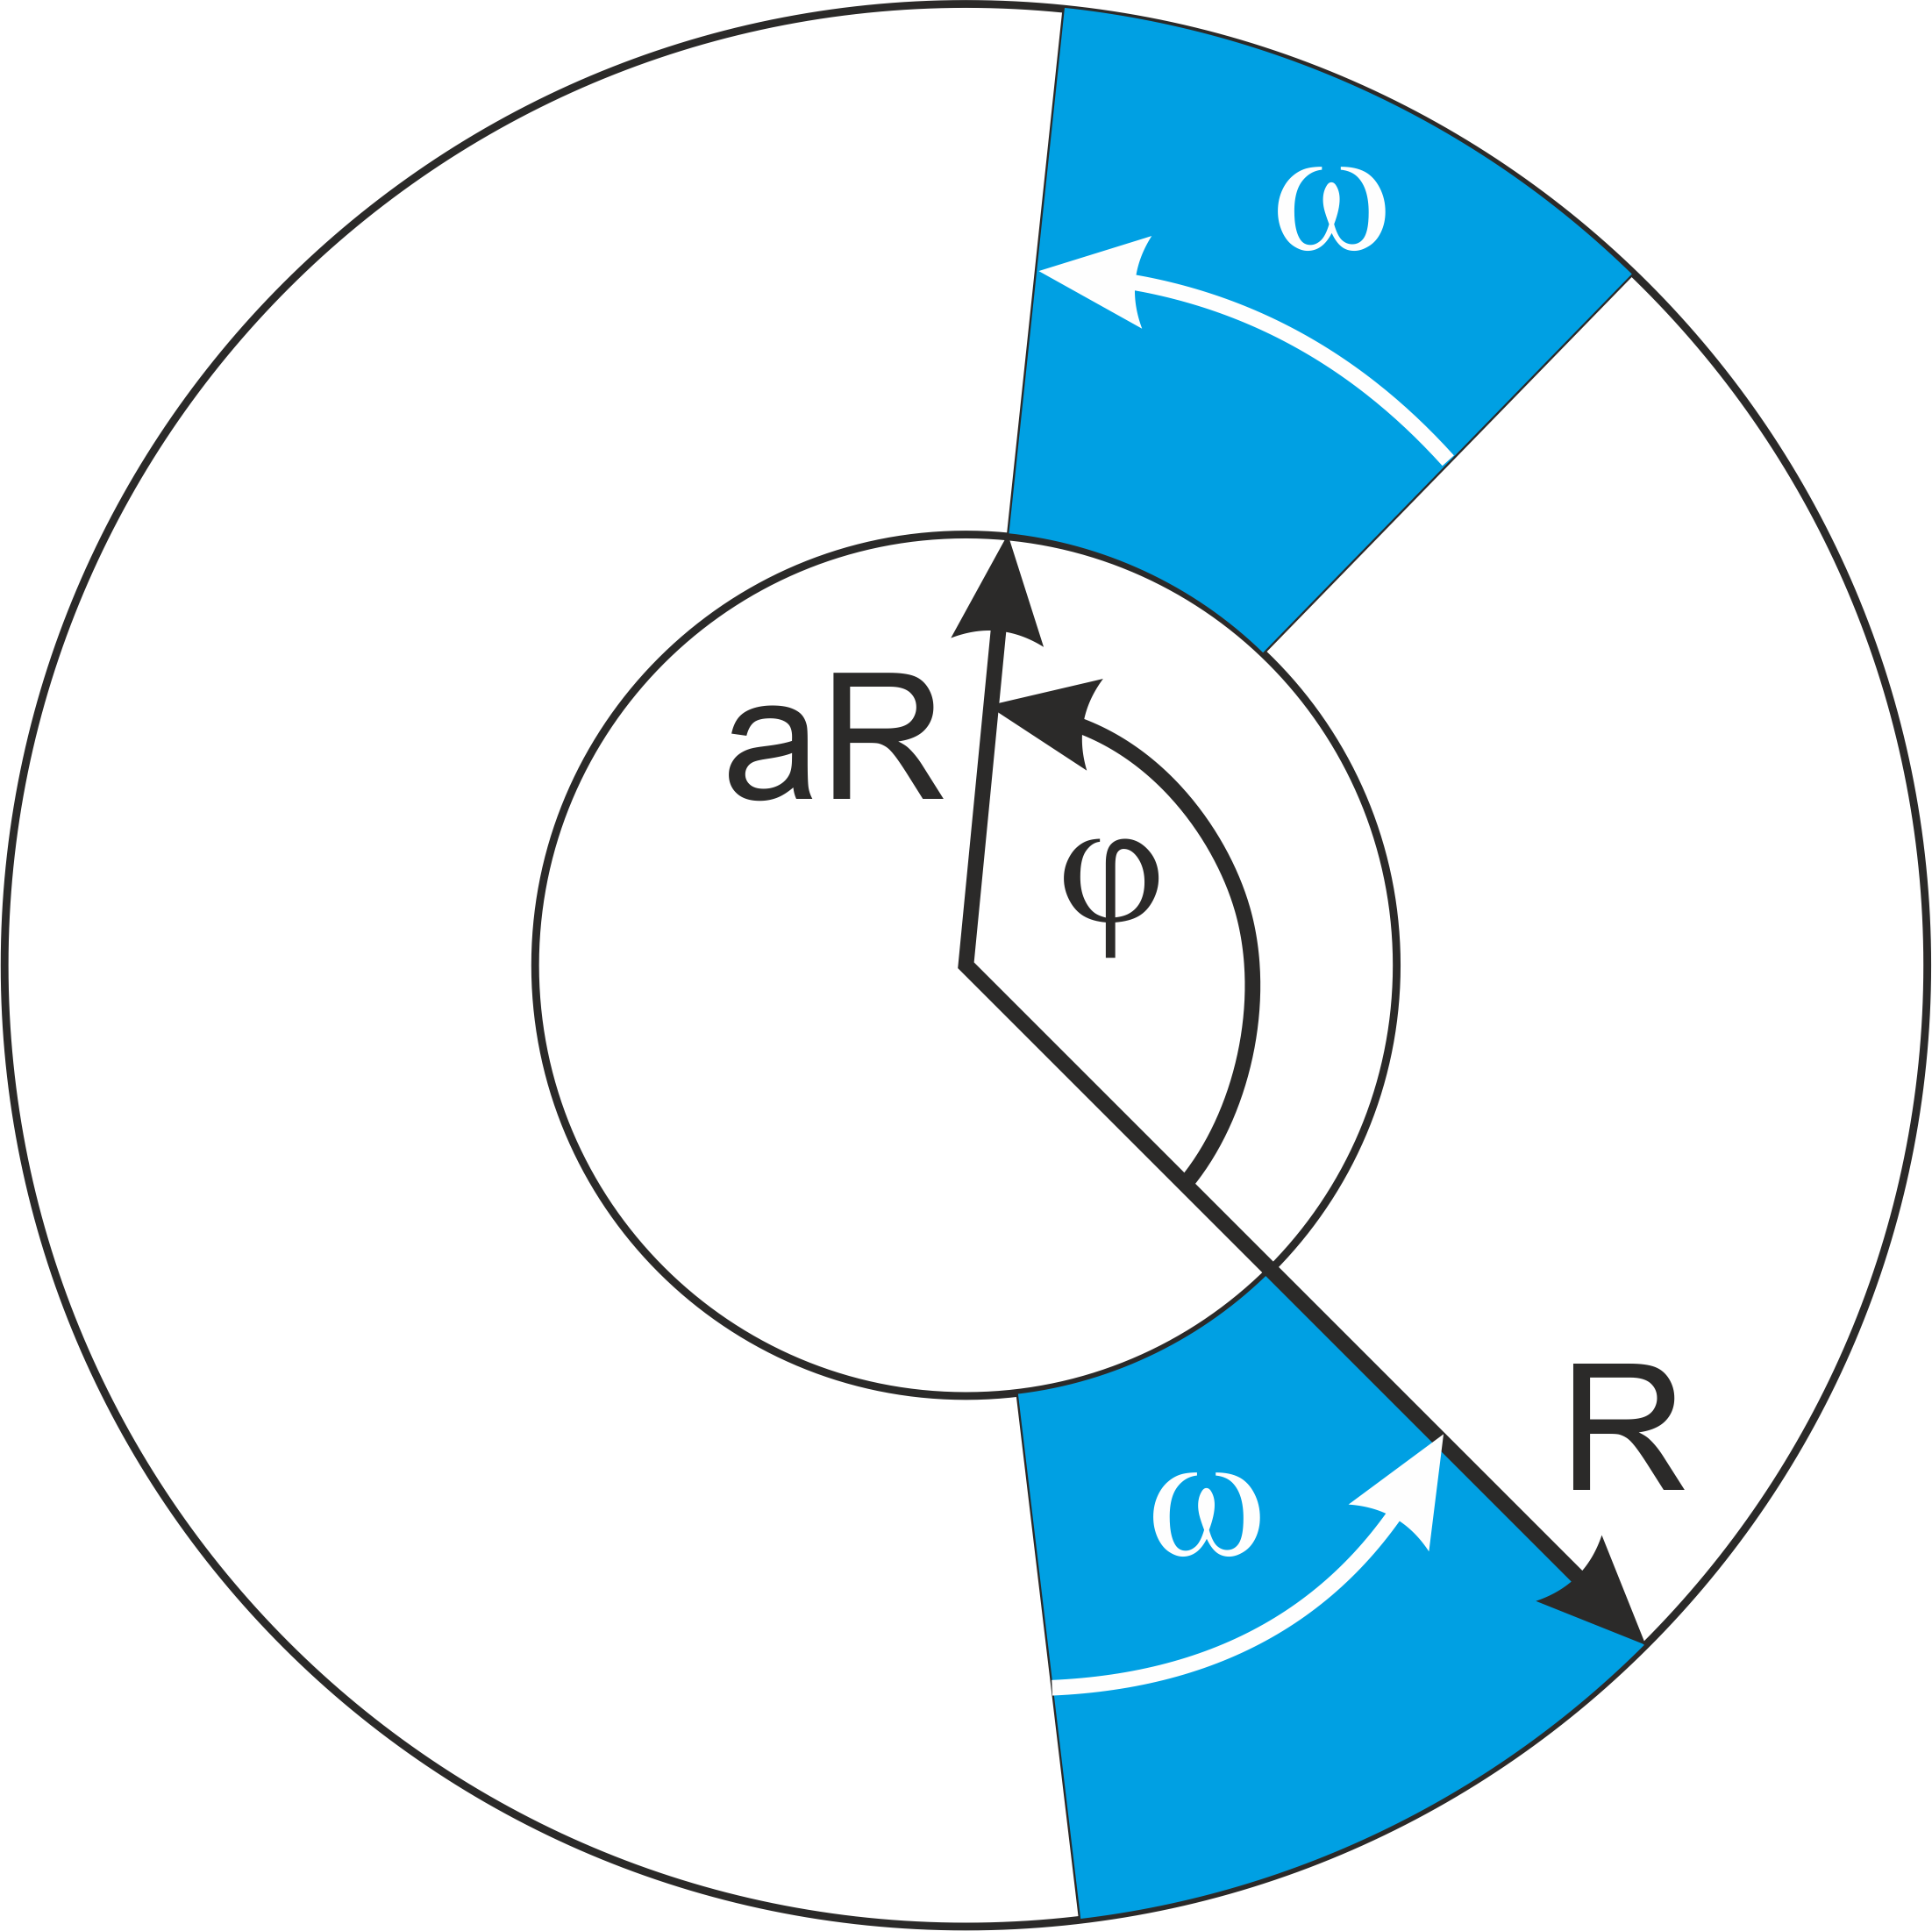
\includegraphics[width=1\textwidth]{../images/form_factor/cylindrical_obj/fanlike_helicesXS.png}
   \caption{top on view}
   \label{fig:fanhelixside1}
\end{subfigure}
\hfill
\begin{subfigure}[b]{.48\textwidth}
   \centering
   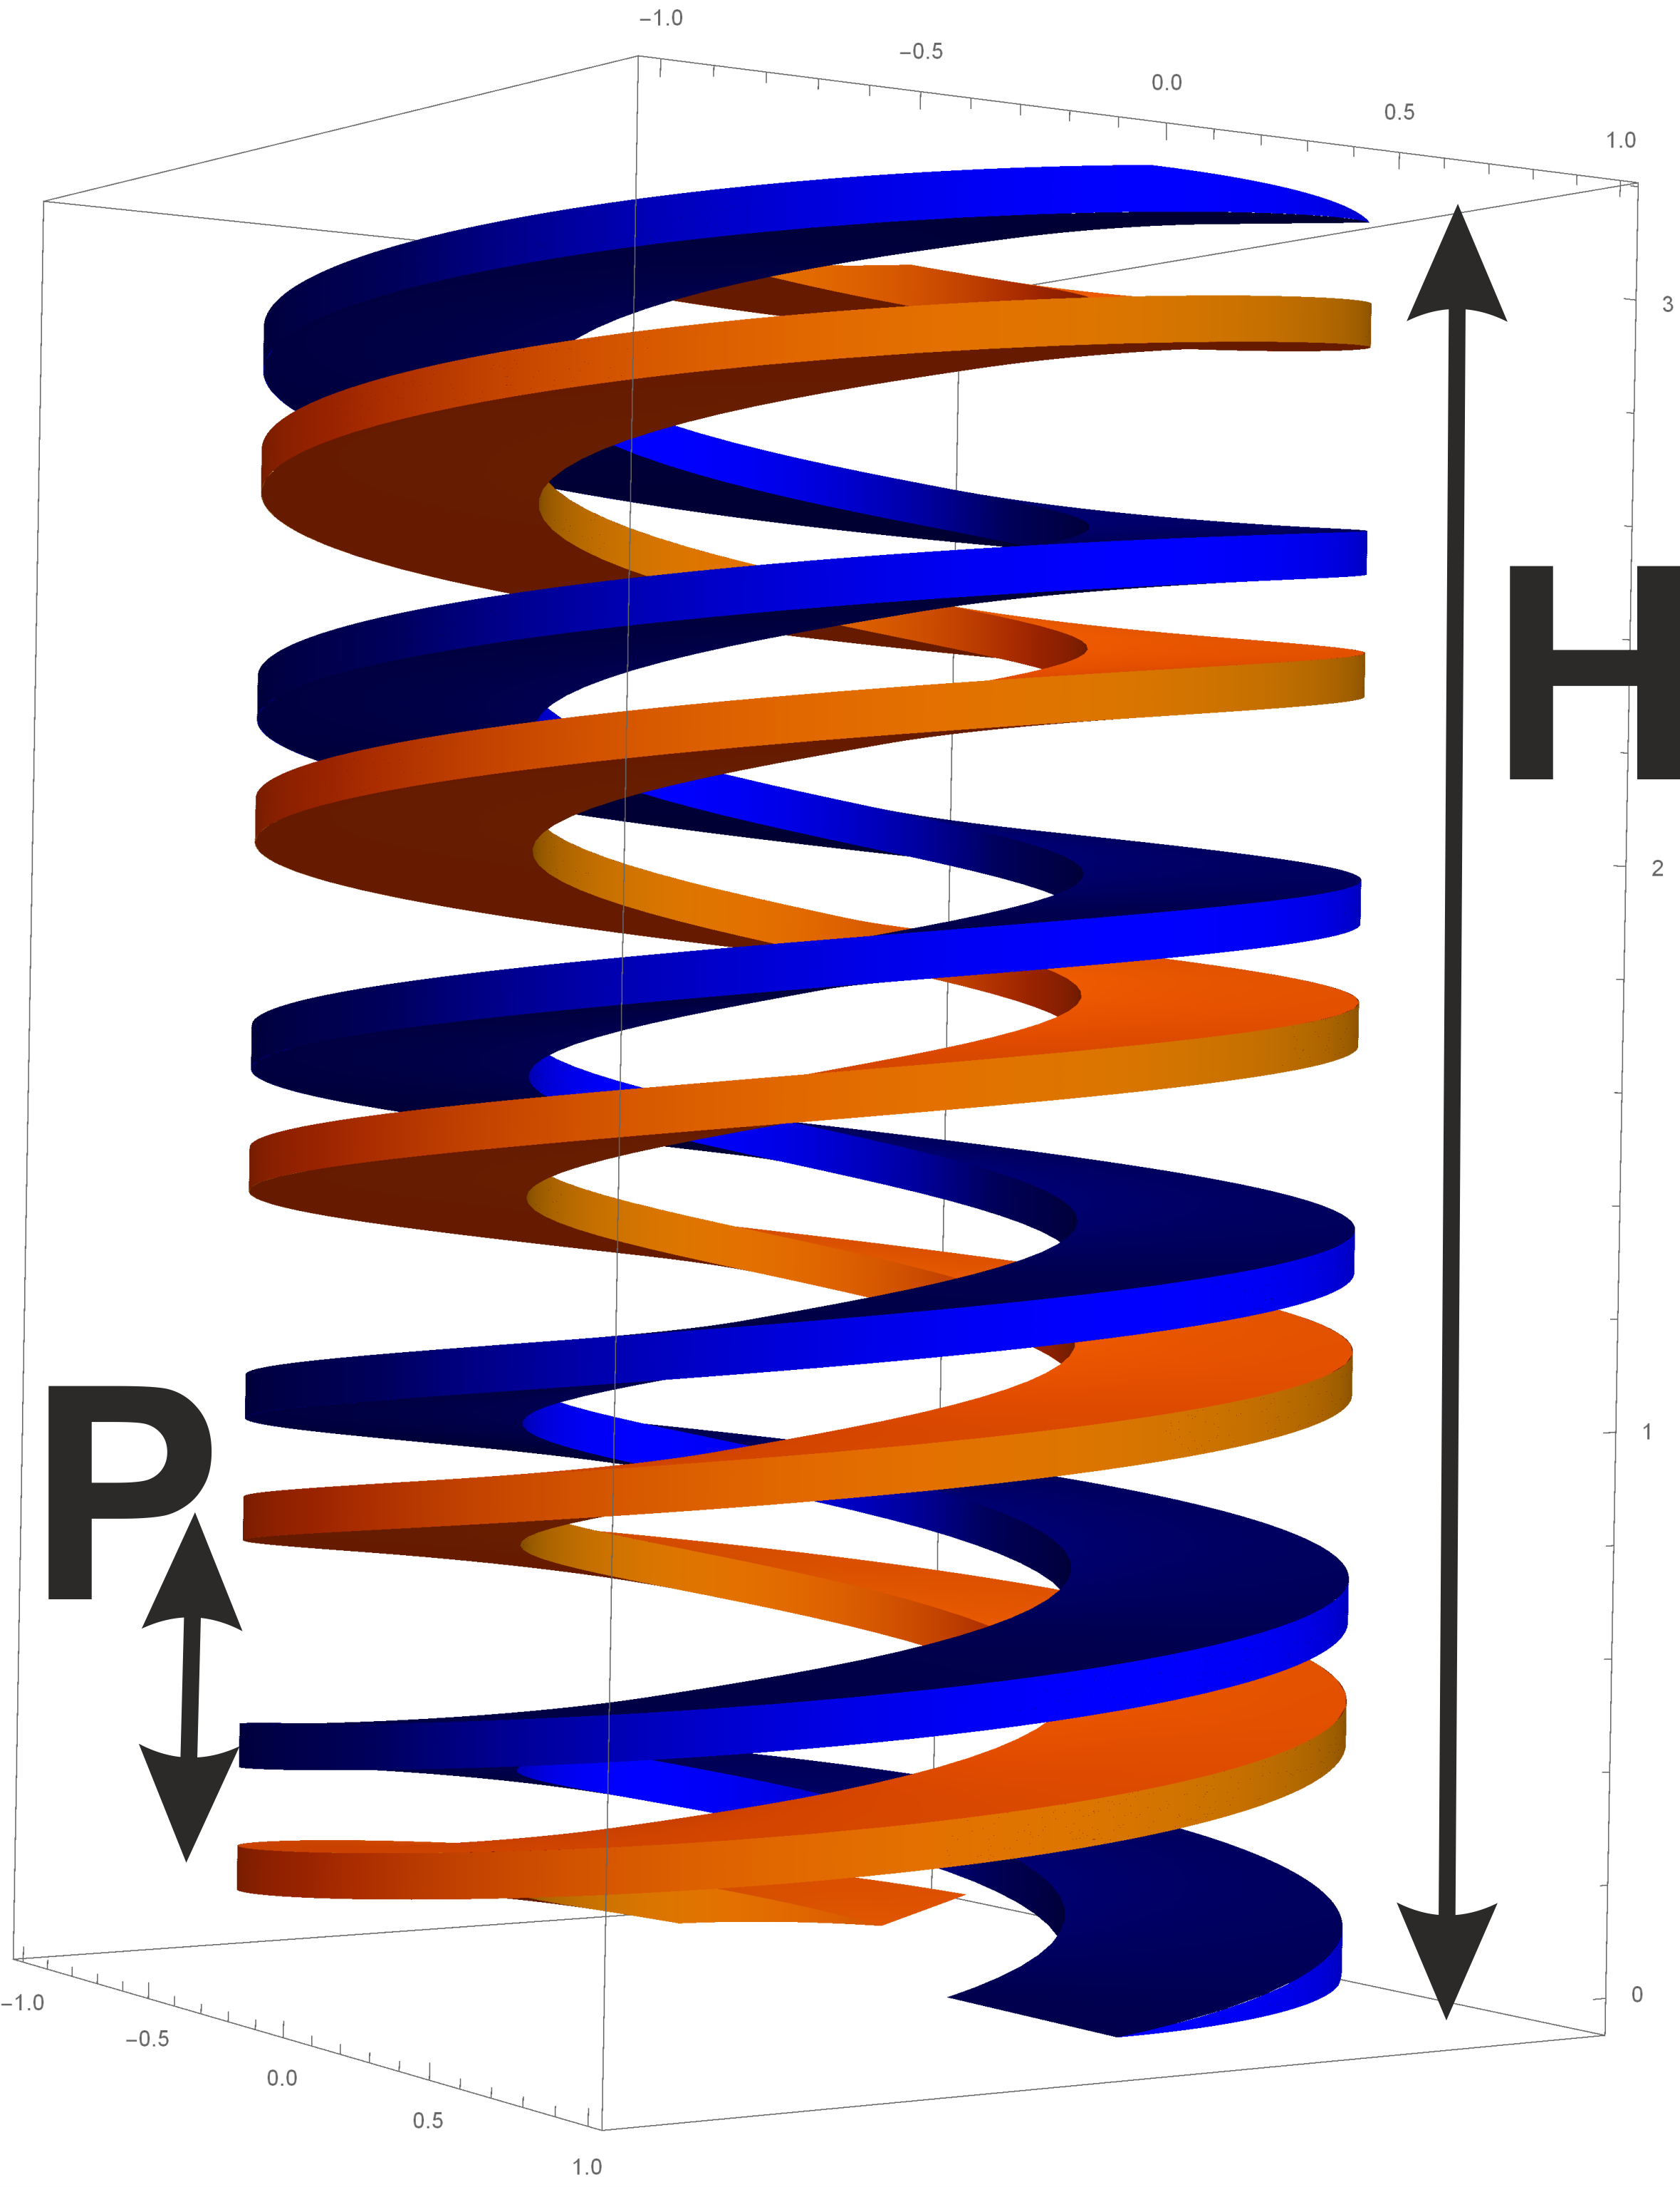
\includegraphics[width=1\textwidth]{../images/form_factor/cylindrical_obj/fanlike_helices3D.png}
   \caption{side view}
   \label{fig:fanhelixside2}
\end{subfigure}
\caption{Double helix with strands of round cross sections.} \label{fig:fanhelix}
\end{figure}

\begin{align}
\begin{split}
I(Q) &= P_\text{rod}(Q,H) \left(\left(\eta_\text{h}-\eta_\text{solv}\right)\omega R^2\left(1-a^2\right)\right)^2 \\
&\times \sum_{n=0}^\infty \epsilon_n \left( \cos(n\varphi/2) \frac{\sin(n\omega/2)}{n\omega/2} g_n\left(Q,R,a\right)\right)^2
\end{split} \\
g_n\left(Q,R,a\right) &= \frac{2}{R^2\left(1-a^2\right)} \int_{aR}^R r' J_n\left(Qr'\left(1-q_n^2\right)\right)\mathrm{d}r' \\
q_n &=
\begin{cases}
\begin{array}{rcl}
\frac{2\pi n}{QP} & \text{for} & Q\geq \frac{2\pi n}{P}\\
1 & \text{for} & Q < \frac{2\pi n}{P}
\end{array}
\end{cases} \\
P_\text{rod}(Q,H) &= H^2 \left(2\frac{\mathrm{Si}(QH)}{(QH)}-\left(\frac{\sin(QH/2)}{QH/2}\right)^2\right)
\end{align}
with $\epsilon_n=1$ for $n=0$ and $\epsilon_n=2$ for $n\geq 1$.

The sum converges very fast and for small $Q$-values the first few terms are already sufficient. However, {\tt SASfit} is continuing the sum until the relative change of the sum is less than $10^{-10}$.

The forward scattering of the model is normalized to the squared scattering length density contrast and squared total volume of the helix so that
\begin{align}
I(Q=0) &= \left(H\left(\eta_\text{h}-\eta_\text{solv}\right)\omega R^2\left(1-a^2\right)\right)^2
\end{align}

\vspace{5mm}

\uline{Input Parameters for model \texttt{fanlike helix}:}\\
\begin{description}
\item[\texttt{R}] external helix radius $R$
\item[\texttt{a}] inner helix radius $aR$, with $0\leq a\leq 1$
\item[\texttt{omega}] angular of the sector of material $\omega$
\item[\texttt{phi}] angle between the two sectors of matrerial $\varphi$
\item[\texttt{dummy}] not used
\item[\texttt{P}] height of one helix period $P$
\item[\texttt{H}] total length of helix $H$
\item[\texttt{eta\_h}] scattering length density of helix $\eta_\text{h}$
\item[\texttt{dummy}] not used
\item[\texttt{eta\_solv}] scattering length density of solvent $\eta_\text{solv}$
\end{description}

\noindent\uline{Note:}
\begin{itemize}
\item The helix is assumed to be stiff and long so that it scattering intensity can be factorized in a cross-section contribution and a shape contribution, whereas the shape contribution can be described by an infinitesimal thin rod of length $H$.
\item $R$, $P$, and $H$ are only physical for values larger than 0.
\item The model is an approximation for the limit $H \gg P$ and $H \gg R$.
\item $0\leq a\leq 1$
\end{itemize}

\begin{figure}[htb]
\begin{center}
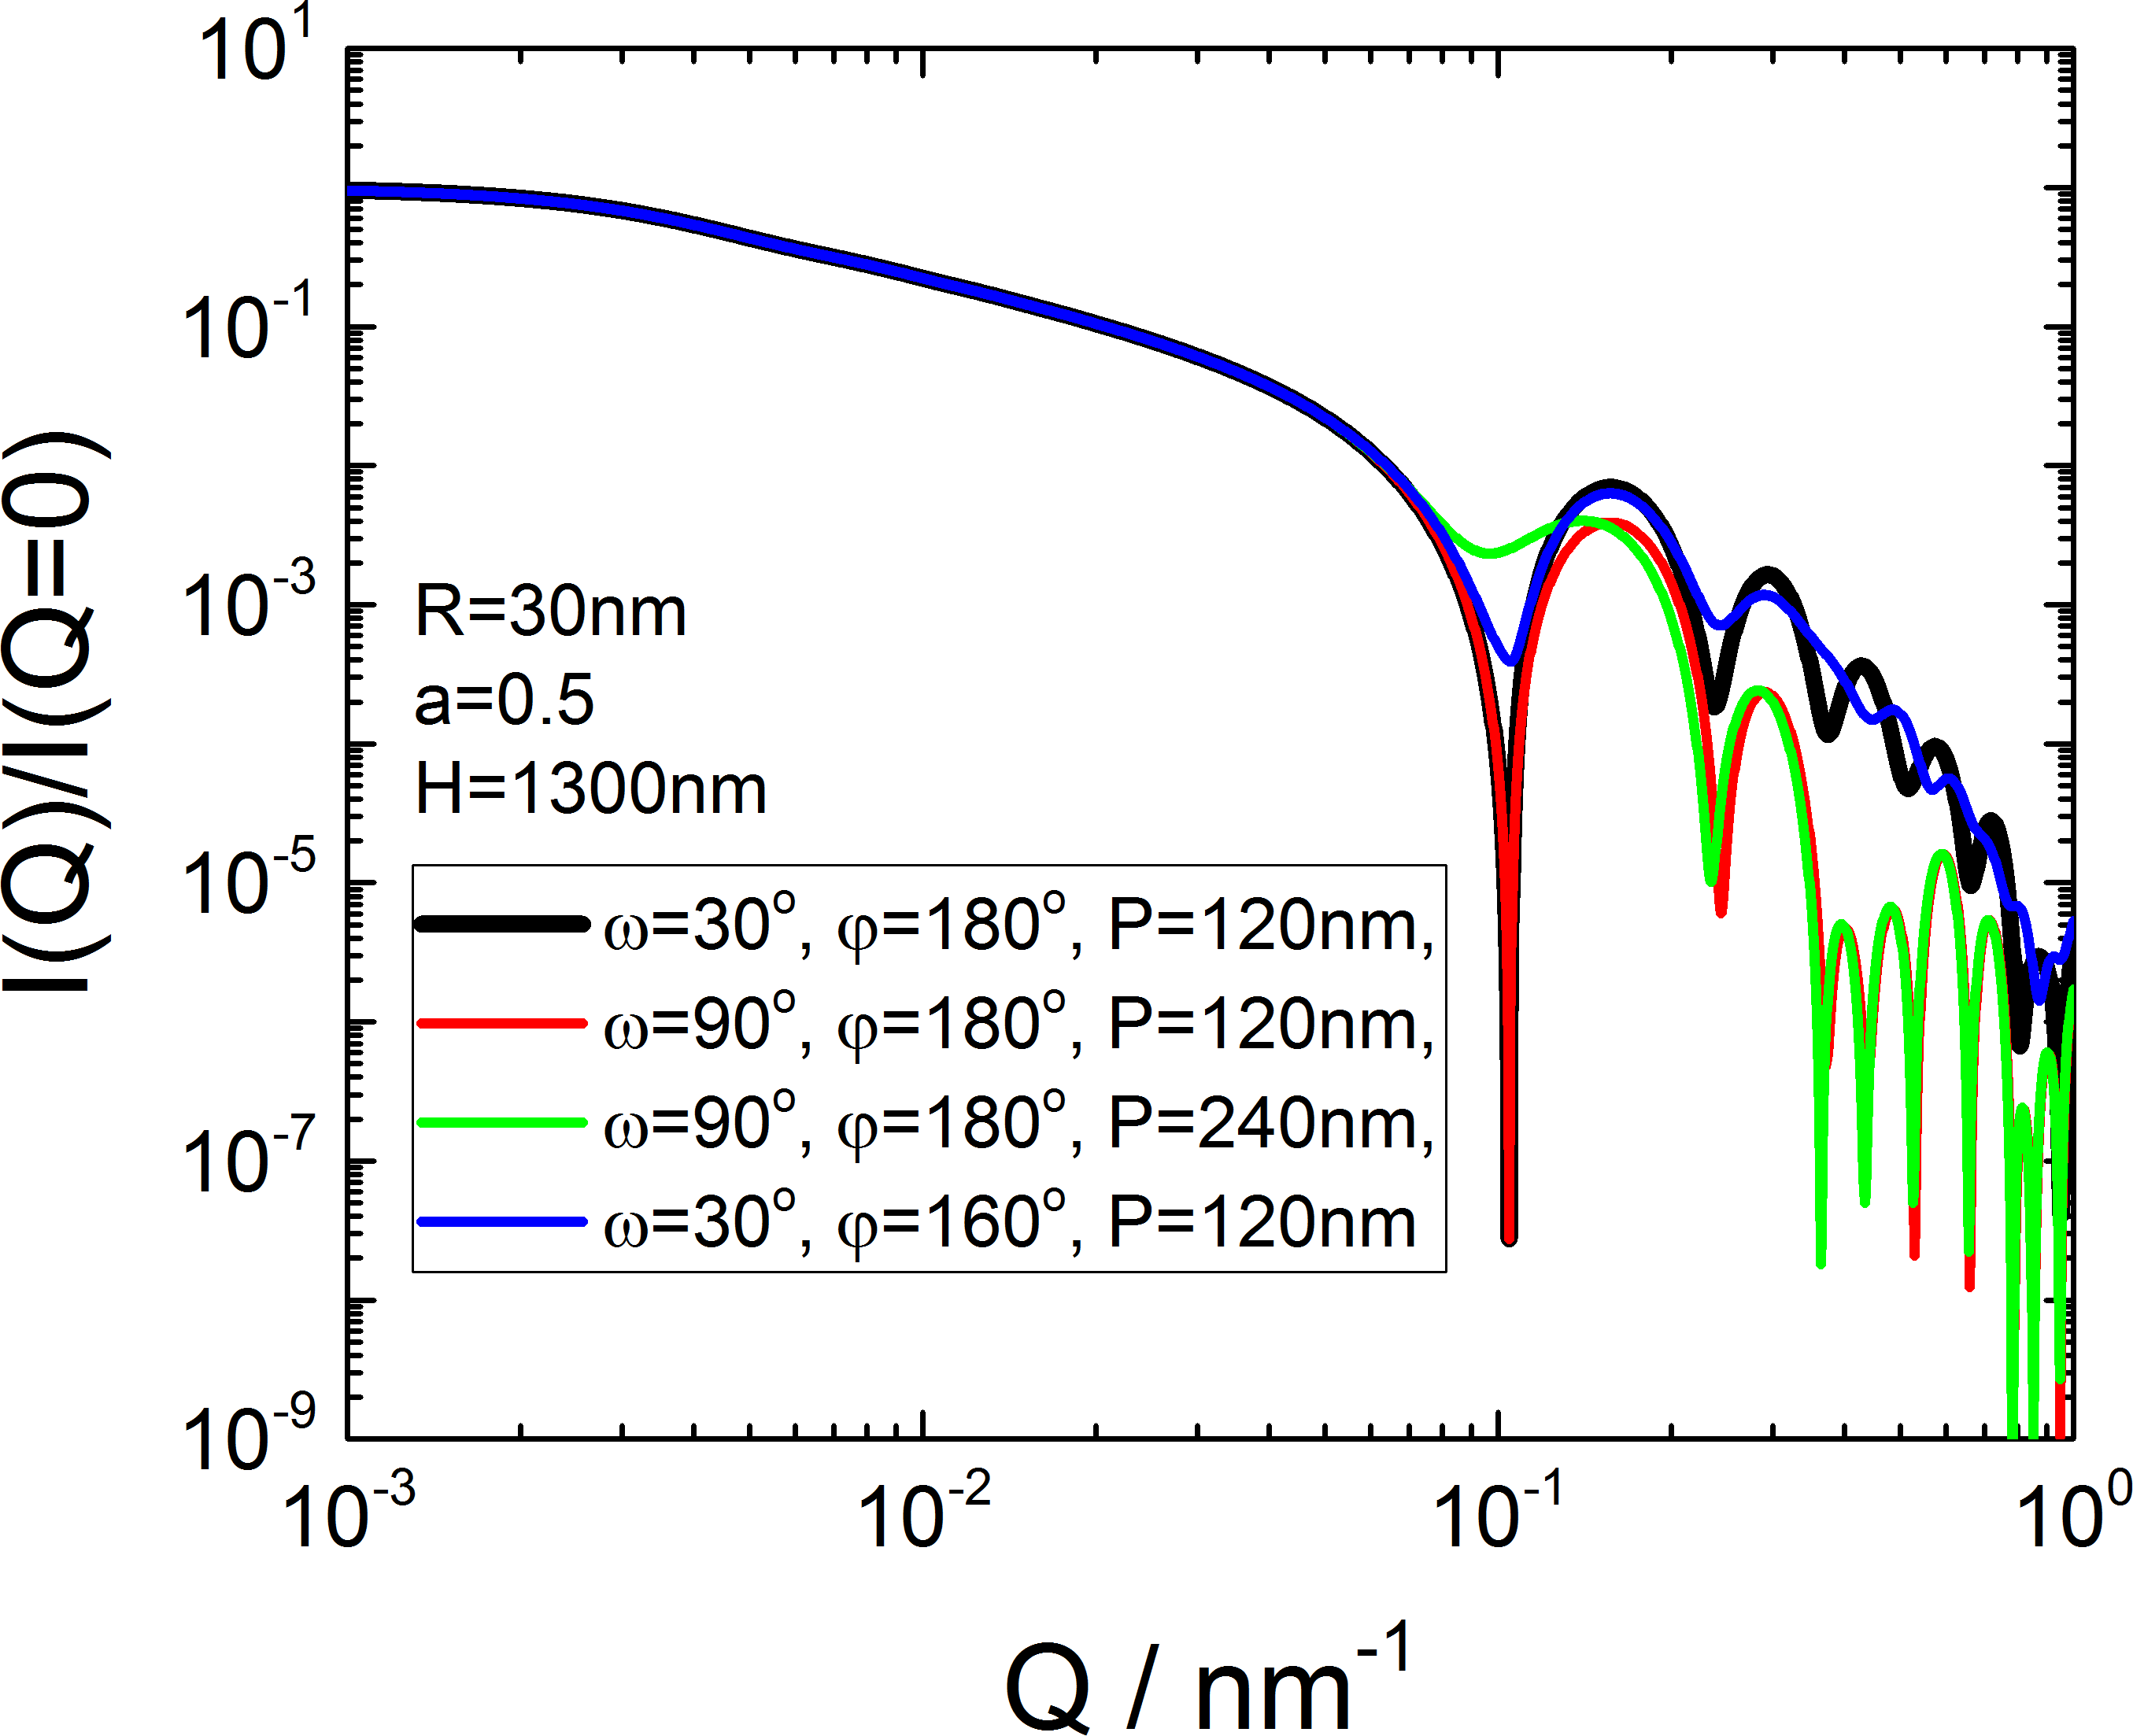
\includegraphics[width=0.7\textwidth]{../images/form_factor/cylindrical_obj/helix_fanlike_IQ.png}
\end{center}
\caption{Normalized scattering curves of fanlike helices.}
\label{fig:helixfanlikeIQ}
\end{figure}

%\phantom{.}~\\
\newpage
\subsubsection{Helix with round cross-section} ~\\
Originally Franklin et al.\ \cite{Franklin1956} and Puigjaner et al.\ \cite{Puigjaner1974} have given the form factor of a cylinder with a groove of a double helix shape of round cross section. Fukada \cite{Fukuda2002} is discussing the form factor of the random oriented double helices alone, but with arbitrary cross-sections.
\begin{figure}[htb]
\begin{subfigure}[b]{.48\textwidth}
   \centering
   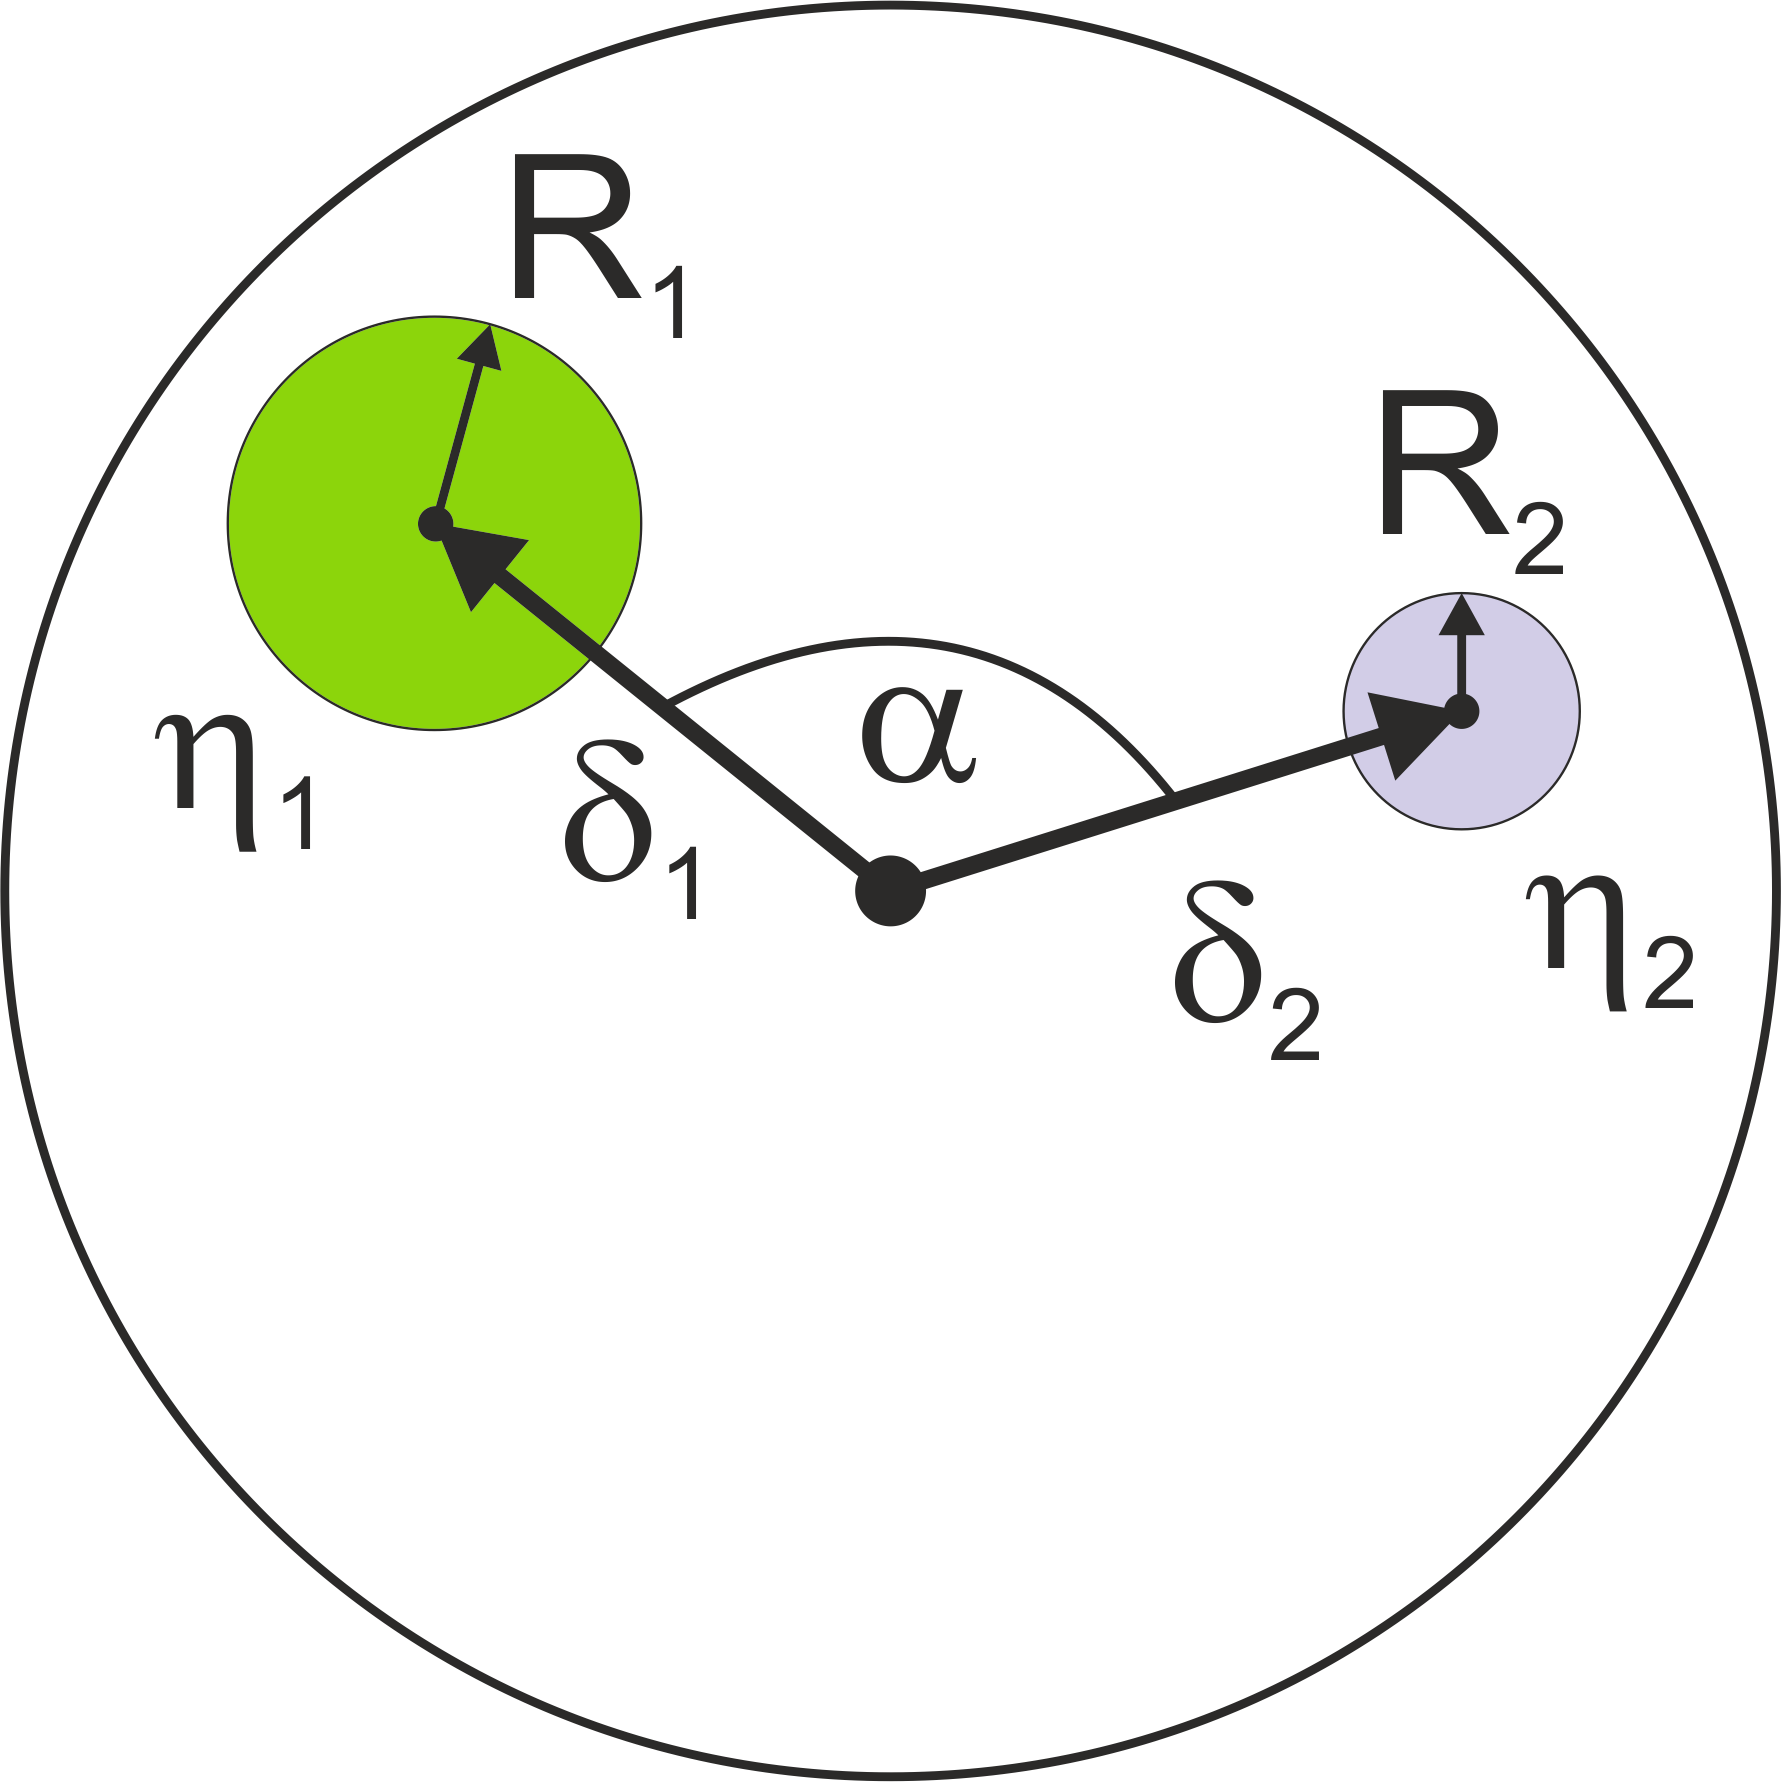
\includegraphics[width=1\textwidth]{../images/form_factor/cylindrical_obj/roundhelices1.png}
   \caption{top on view}
   \label{fig:roundhelix1}
\end{subfigure}
\hfill
\begin{subfigure}[b]{.48\textwidth}
   \centering
   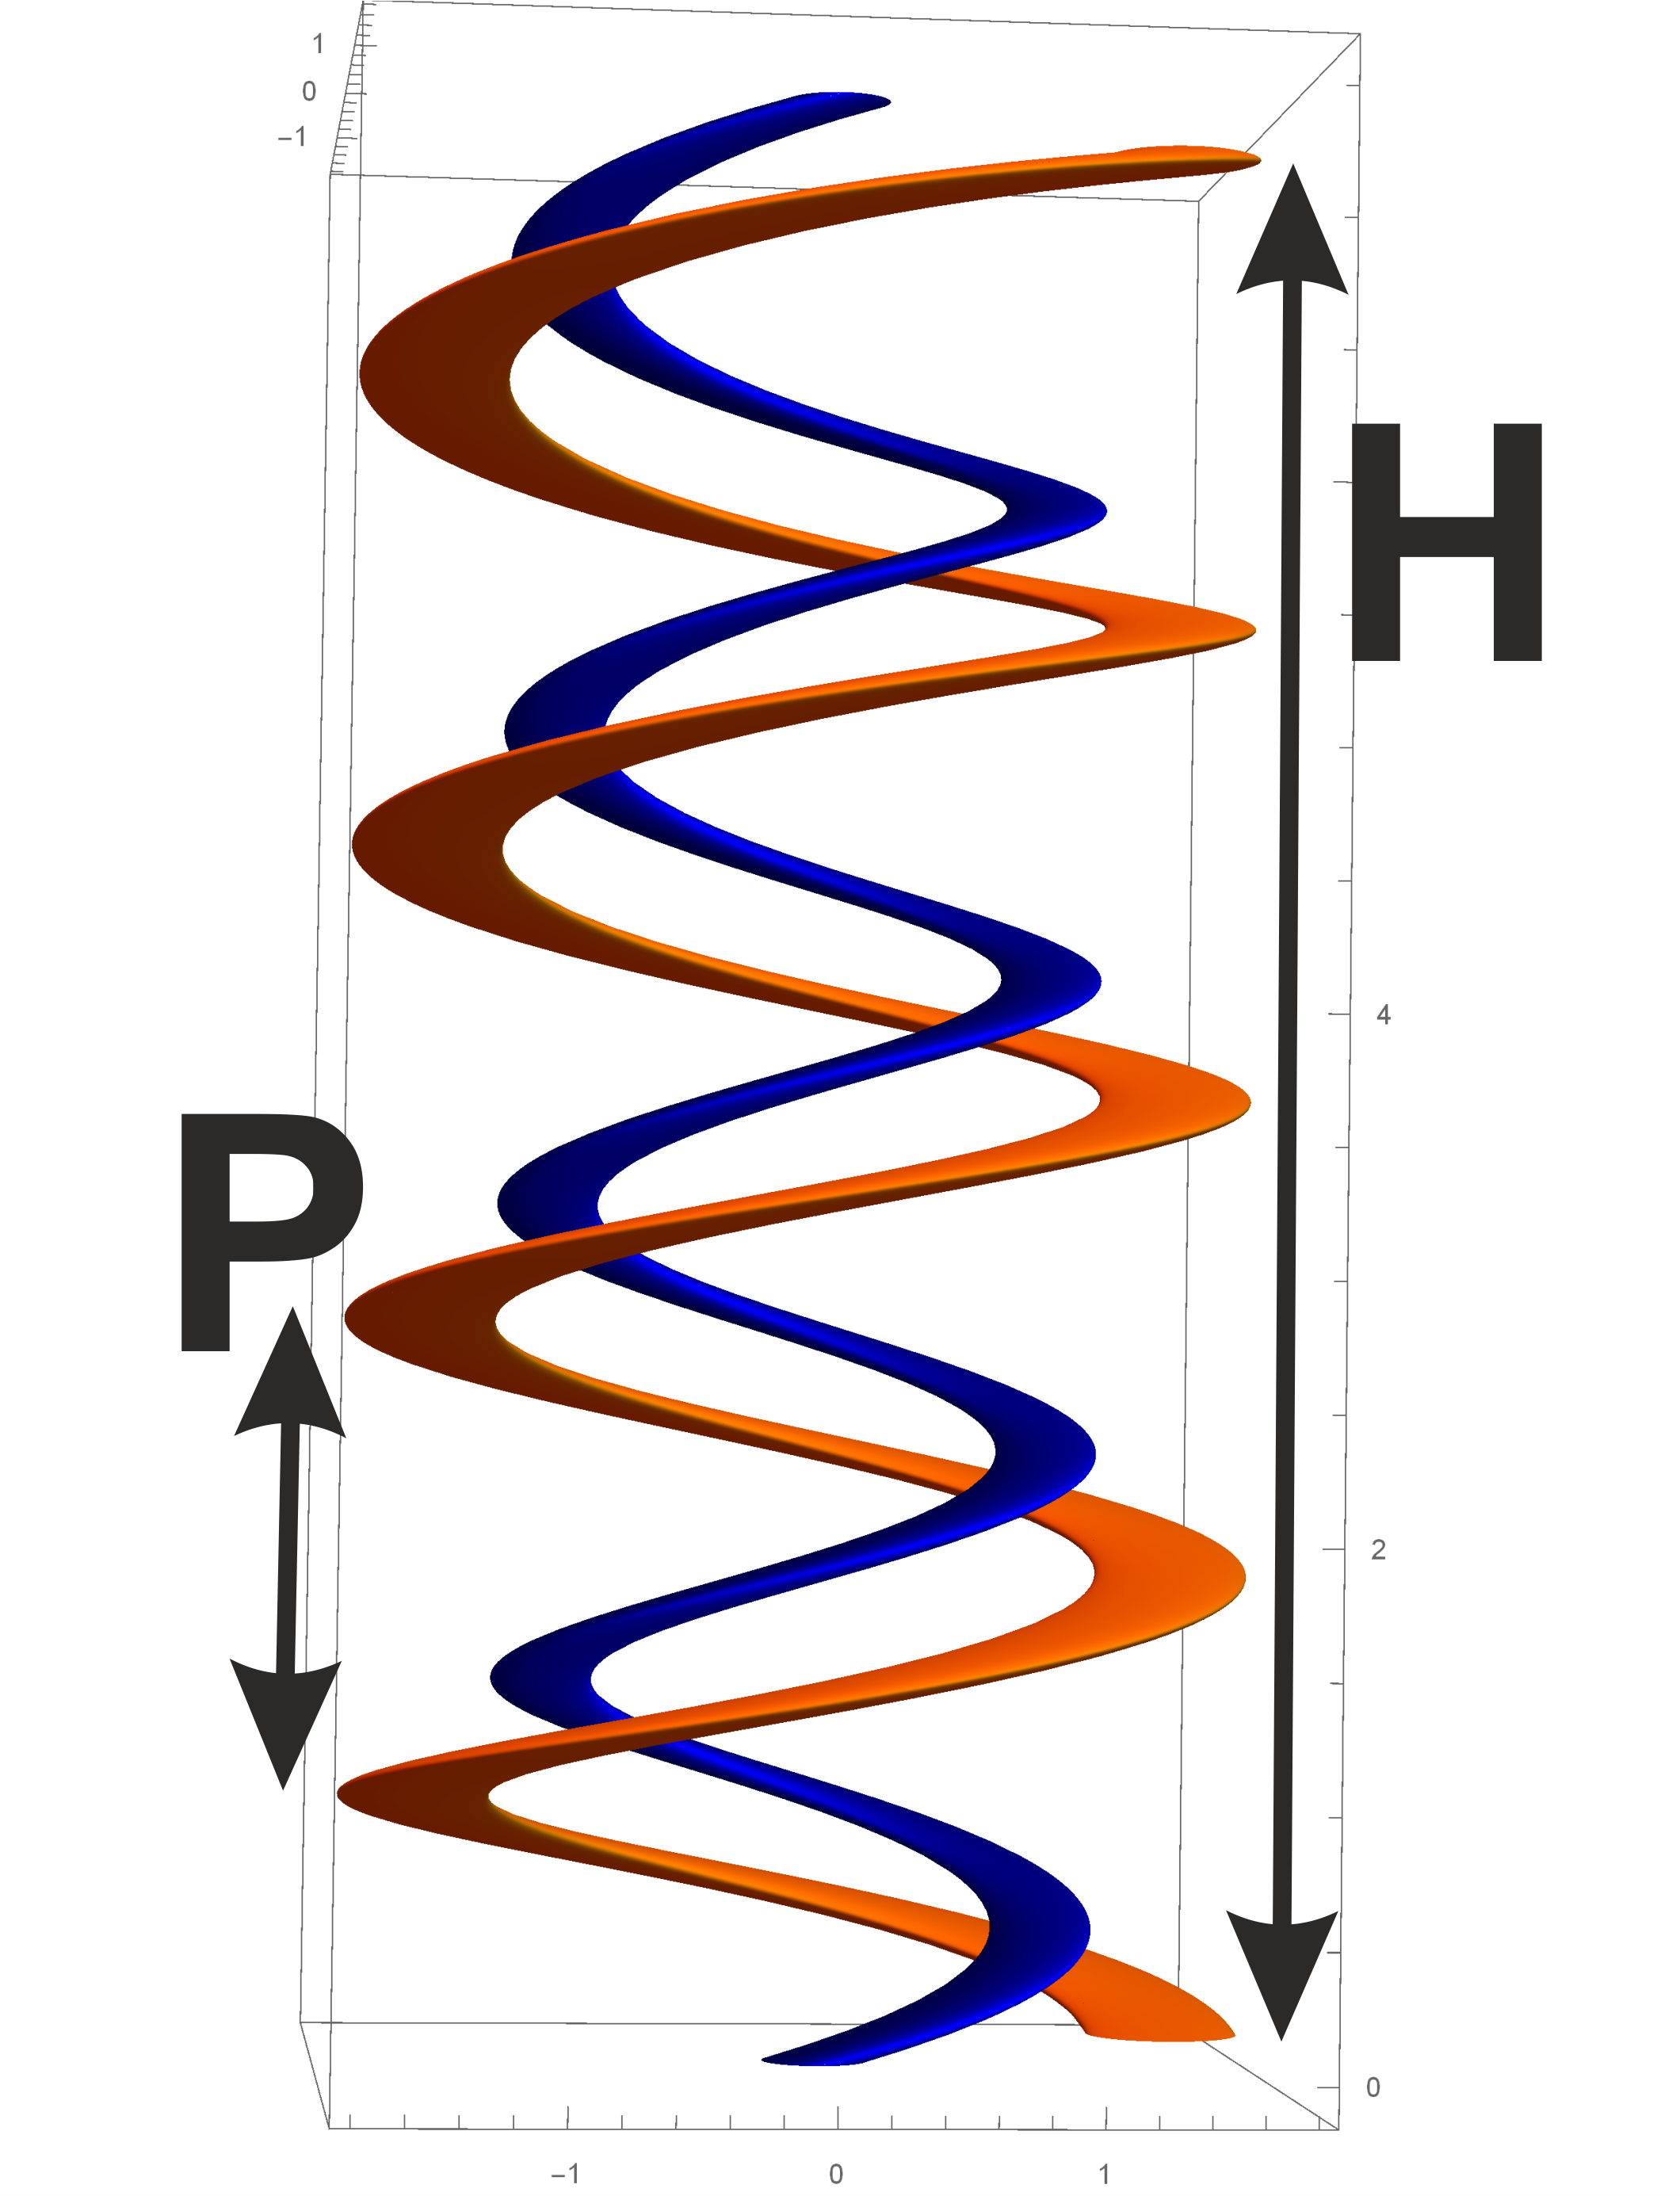
\includegraphics[width=1\textwidth]{../images/form_factor/cylindrical_obj/round_helices3D.png}
   \caption{side view}
   \label{fig:roundhelix2}
\end{subfigure}
\caption{Double helix with strands of round cross sections. The cross-sections are round in the plane perpendicular to the helix axis.} \label{fig:roundhelix}
\end{figure}

\begin{align}
I(Q) &= P_\text{rod}(Q,H) \sum_{n=0}^{\infty} \epsilon_n \left( A_{1n}^2 + A_{2n}^2+2A_{1n}A_{2n}\cos n\alpha\right)
\label{eq:roundhelix1}
\end{align}
where
\begin{align}
A_{in} &= J_n\left(\delta_i Q_\perp\right) \pi R_i^2 \left(\eta_i-\eta_\mathrm{solv}\right)\frac{2J_1\left(R_i Q_\perp\right)}{R_i Q_\perp} \\
Q_\perp^2 &= Q^2-\left[\frac{2\pi n}{P}\right]^2
\end{align}
with $\epsilon_j=1$ for $j=0$ and $\epsilon_j=2$ for $j\geq 1$. Furthermore $R_1$ and $R_2$ are the radii of the round helical strands.
$\delta_1$ and $\delta_2$ are the distances of the strands to the helix axis.
The pitch of the helix is denoted by $P$, whereas $\alpha$ is the angle between the two strands.

The sum converges very fast and for small $Q$-values the first few terms are already sufficient. However, {\tt SASfit} is continuing the sum until the relative change of the sum is less than $10^{-10}$.

The forward scattering of the model is normalized to the squared scattering length density contrast and squared total volume of the helix so that
\begin{align}
I(Q=0) &= H^2\left(\left(\eta_\text{1}-\eta_\text{solv}\right)\pi R_1^2+\left(\eta_\text{2}-\eta_\text{solv}\right)\pi R_2^2\right)^2
\end{align}

\vspace{5mm}

\uline{Input Parameters for model \texttt{helix with round XS}:}\\
\begin{description}
\item[\texttt{R\_1}] radius of first strand thickness $R_1$
\item[\texttt{delta\_1}] distance of first strand to helix axis $\delta_1$
\item[\texttt{R\_2}] radius of second strand thickness $R_2$
\item[\texttt{delta\_2}] distance of second strand to helix axis $\delta_2$
\item[\texttt{alpha}] angle $\alpha$ between the two strands
\item[\texttt{P}] height of one helix period $P$
\item[\texttt{H}] total length of helix $H$
\item[\texttt{eta\_1}] scattering length density of first strand $\eta_1$
\item[\texttt{eta\_2}] scattering length density of second strand $\eta_2$
\item[\texttt{eta\_solv}] scattering length density of solvent $\eta_\text{solv}$
\end{description}

\noindent\uline{Note:}
\begin{itemize}
\item The helix is assumed to be stiff and long so that it scattering intensity can be factorized in a cross-section contribution and a shape contribution, whereas the shape contribution can be described by an infinitesimal thin rod of length $H$.
\item $R_1$, $R_2$, $\delta_1$, $\delta_2$ $P$, and $H$ are only physical for values larger than 0.
\item The model is an approximation for the limit $H \gg P$ and $H \gg R$.
\end{itemize}

\begin{figure}[htb]
\begin{center}
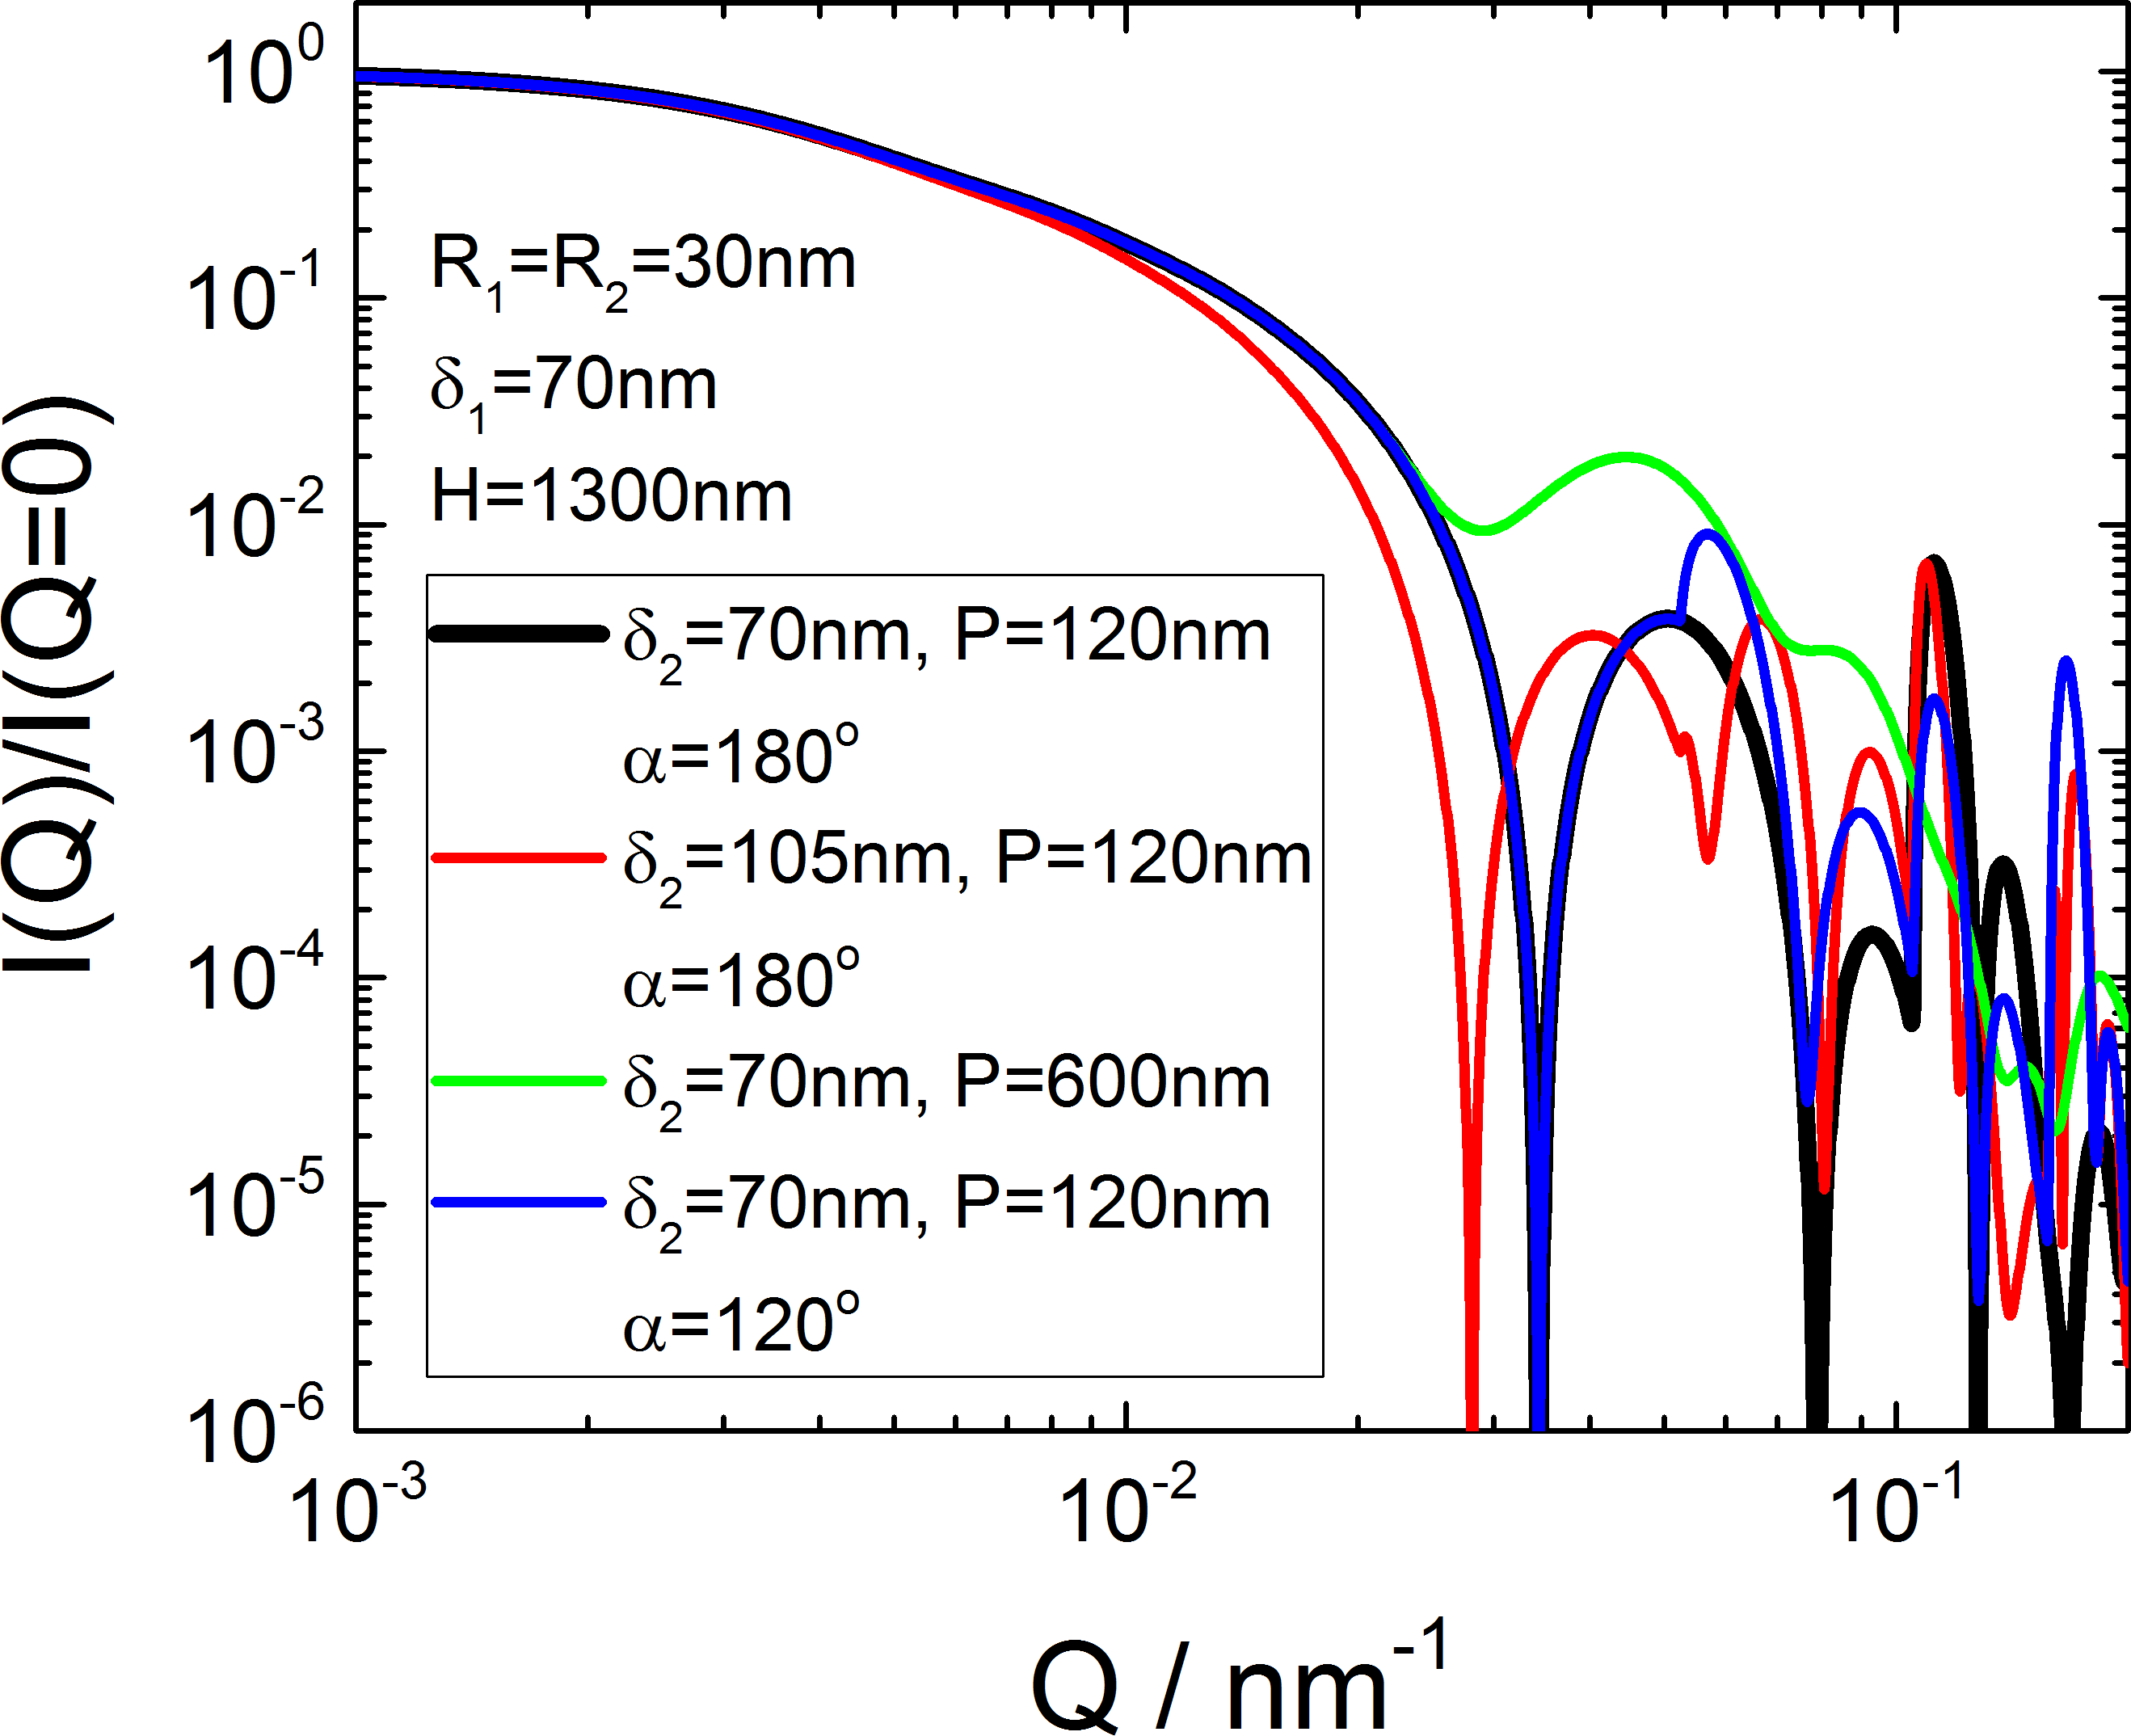
\includegraphics[width=0.7\textwidth]{../images/form_factor/cylindrical_obj/helix_round_IQ.png}
\end{center}
\caption{Normalized scattering curves of helices with round cross sections.}
\label{fig:helixroundIQ}
\end{figure}

%\phantom{.}~\\
\newpage
\subsubsection{Beads model of a single helical strand} ~\\
In this model  \cite{Lebedev2003,Avdeev2013} it is assumed that spherical beads are arranged along the path of a single helical strand. It is the product of the form factor of a sphere and the structure factor described by a helix with an infinitesimal thin single strand.

\begin{figure}[htb]
\begin{subfigure}[b]{.48\textwidth}
   \centering
   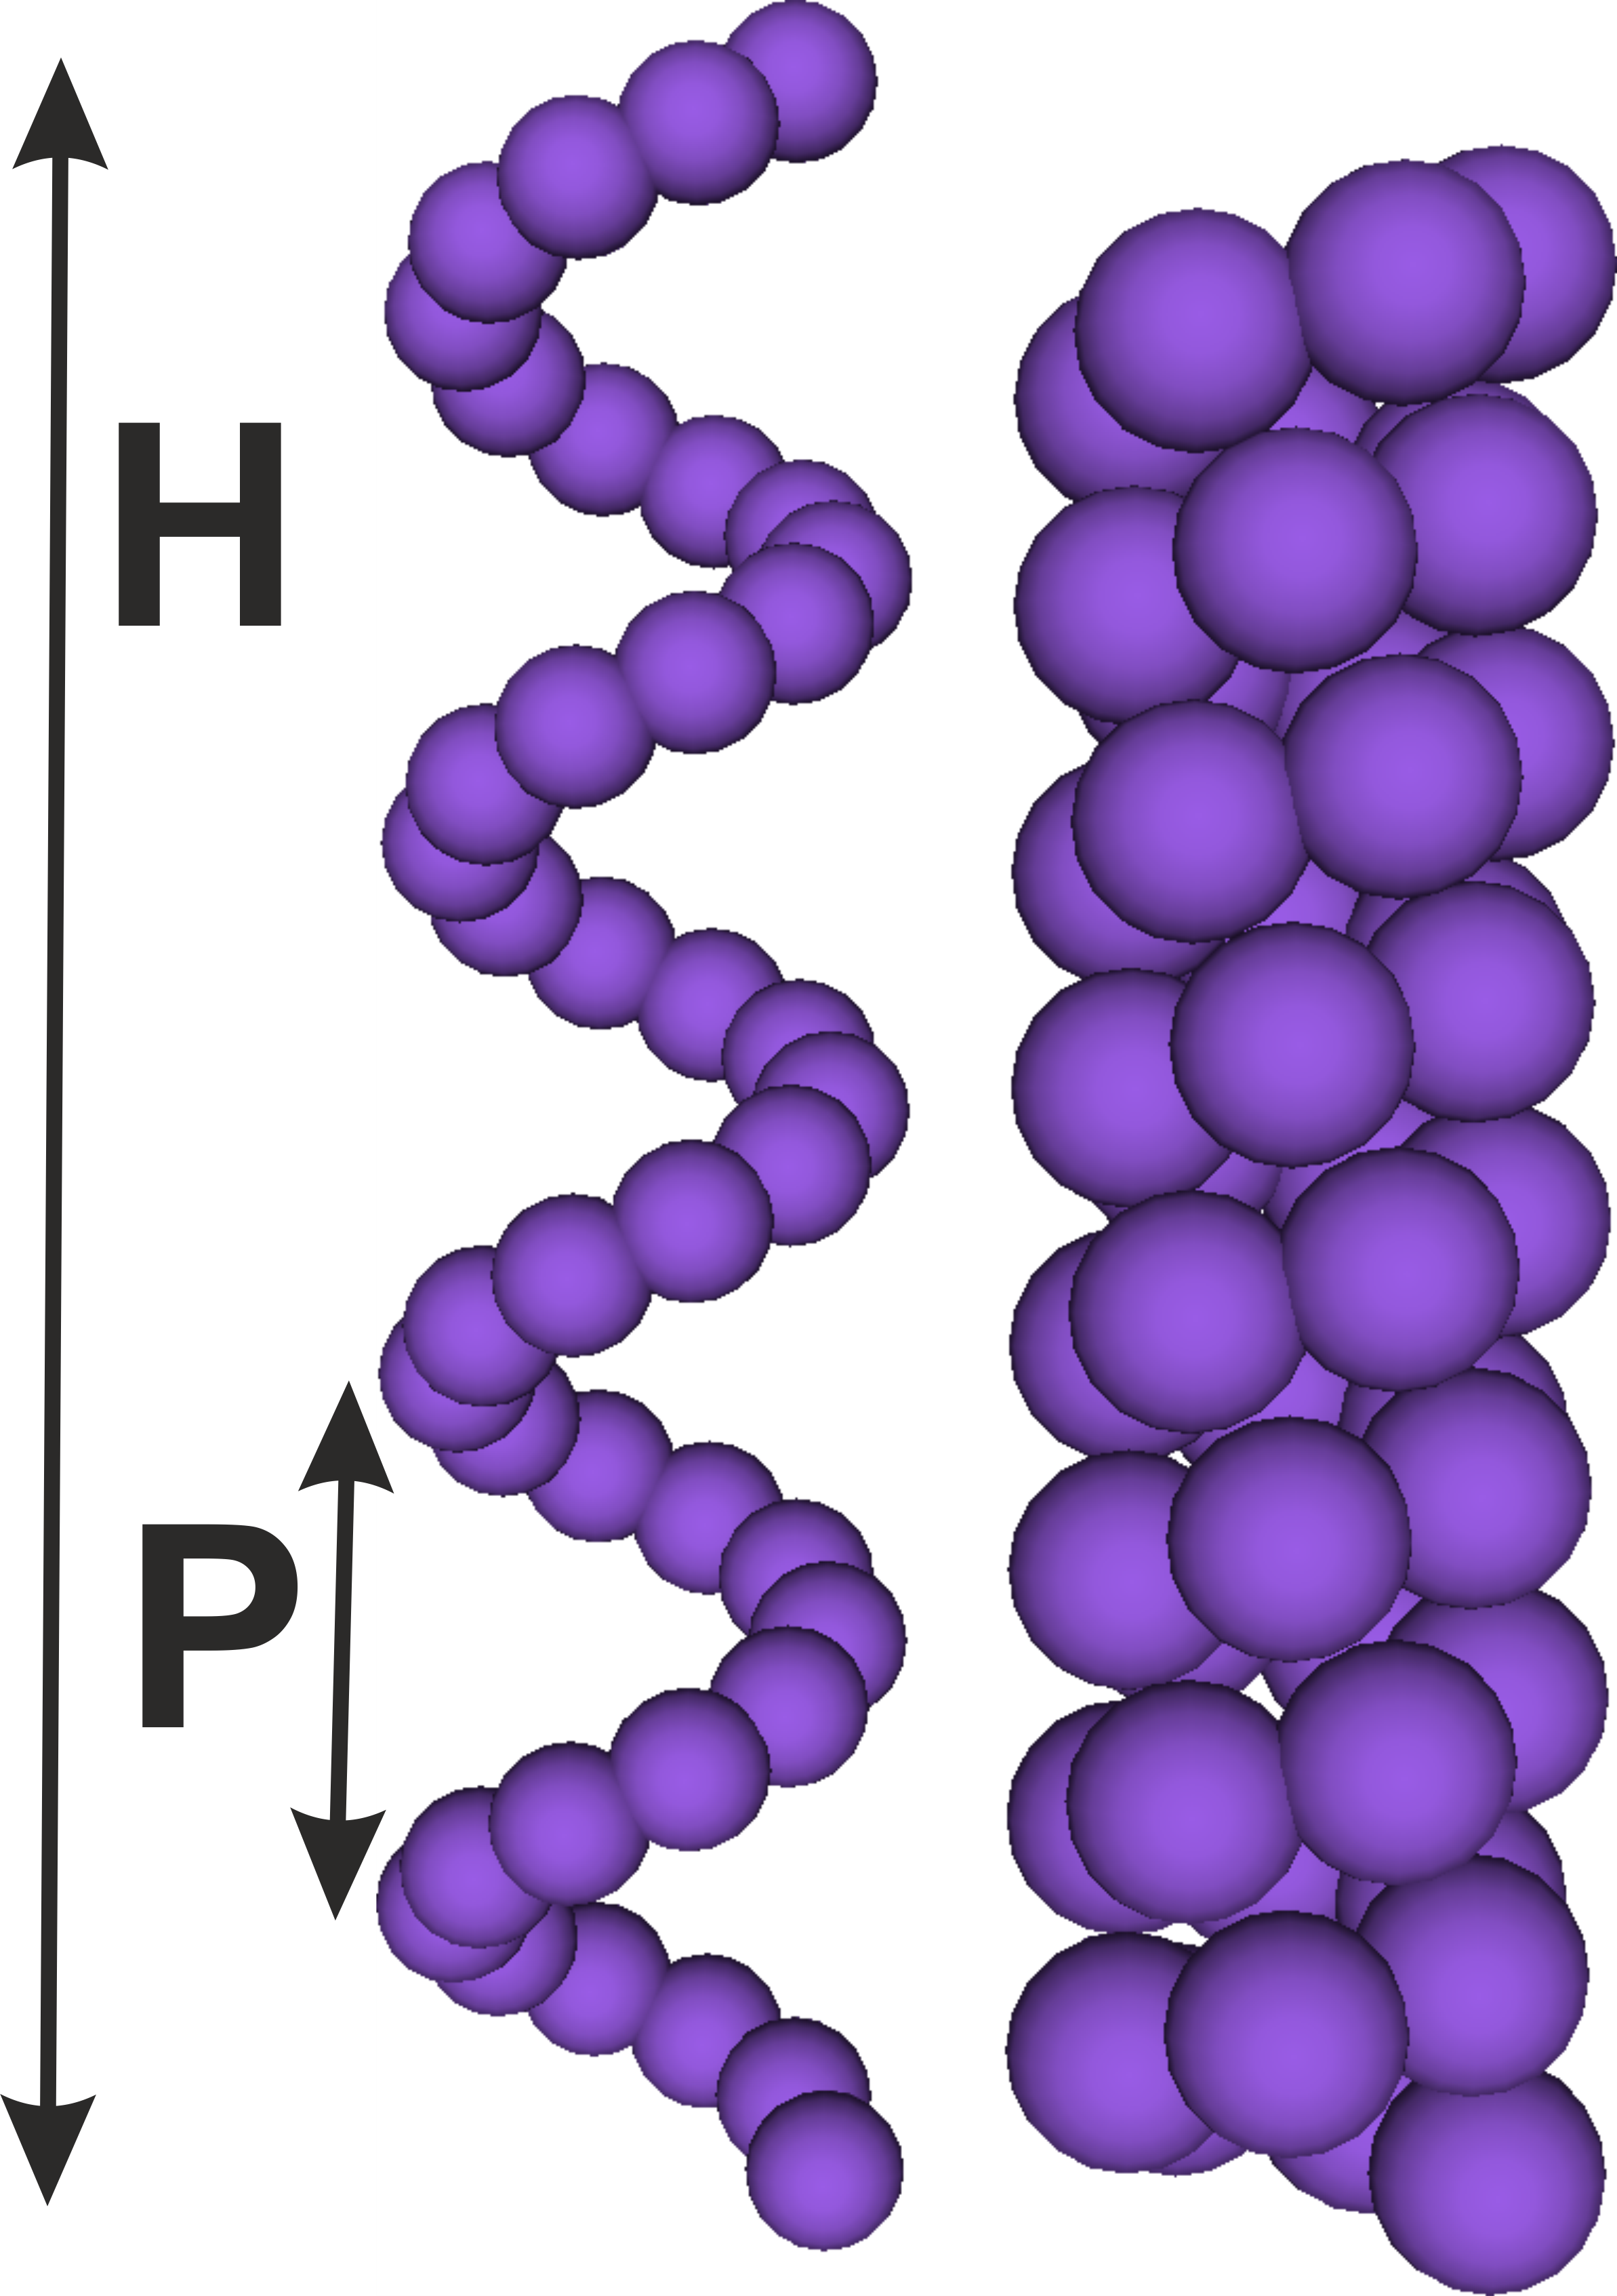
\includegraphics[width=0.9\textwidth]{../images/form_factor/cylindrical_obj/beads_helix_model_1.png}
   \caption{side view}
   \label{fig:beadshelixside1}
\end{subfigure}
\hfill
\begin{subfigure}[b]{.48\textwidth}
   \centering
   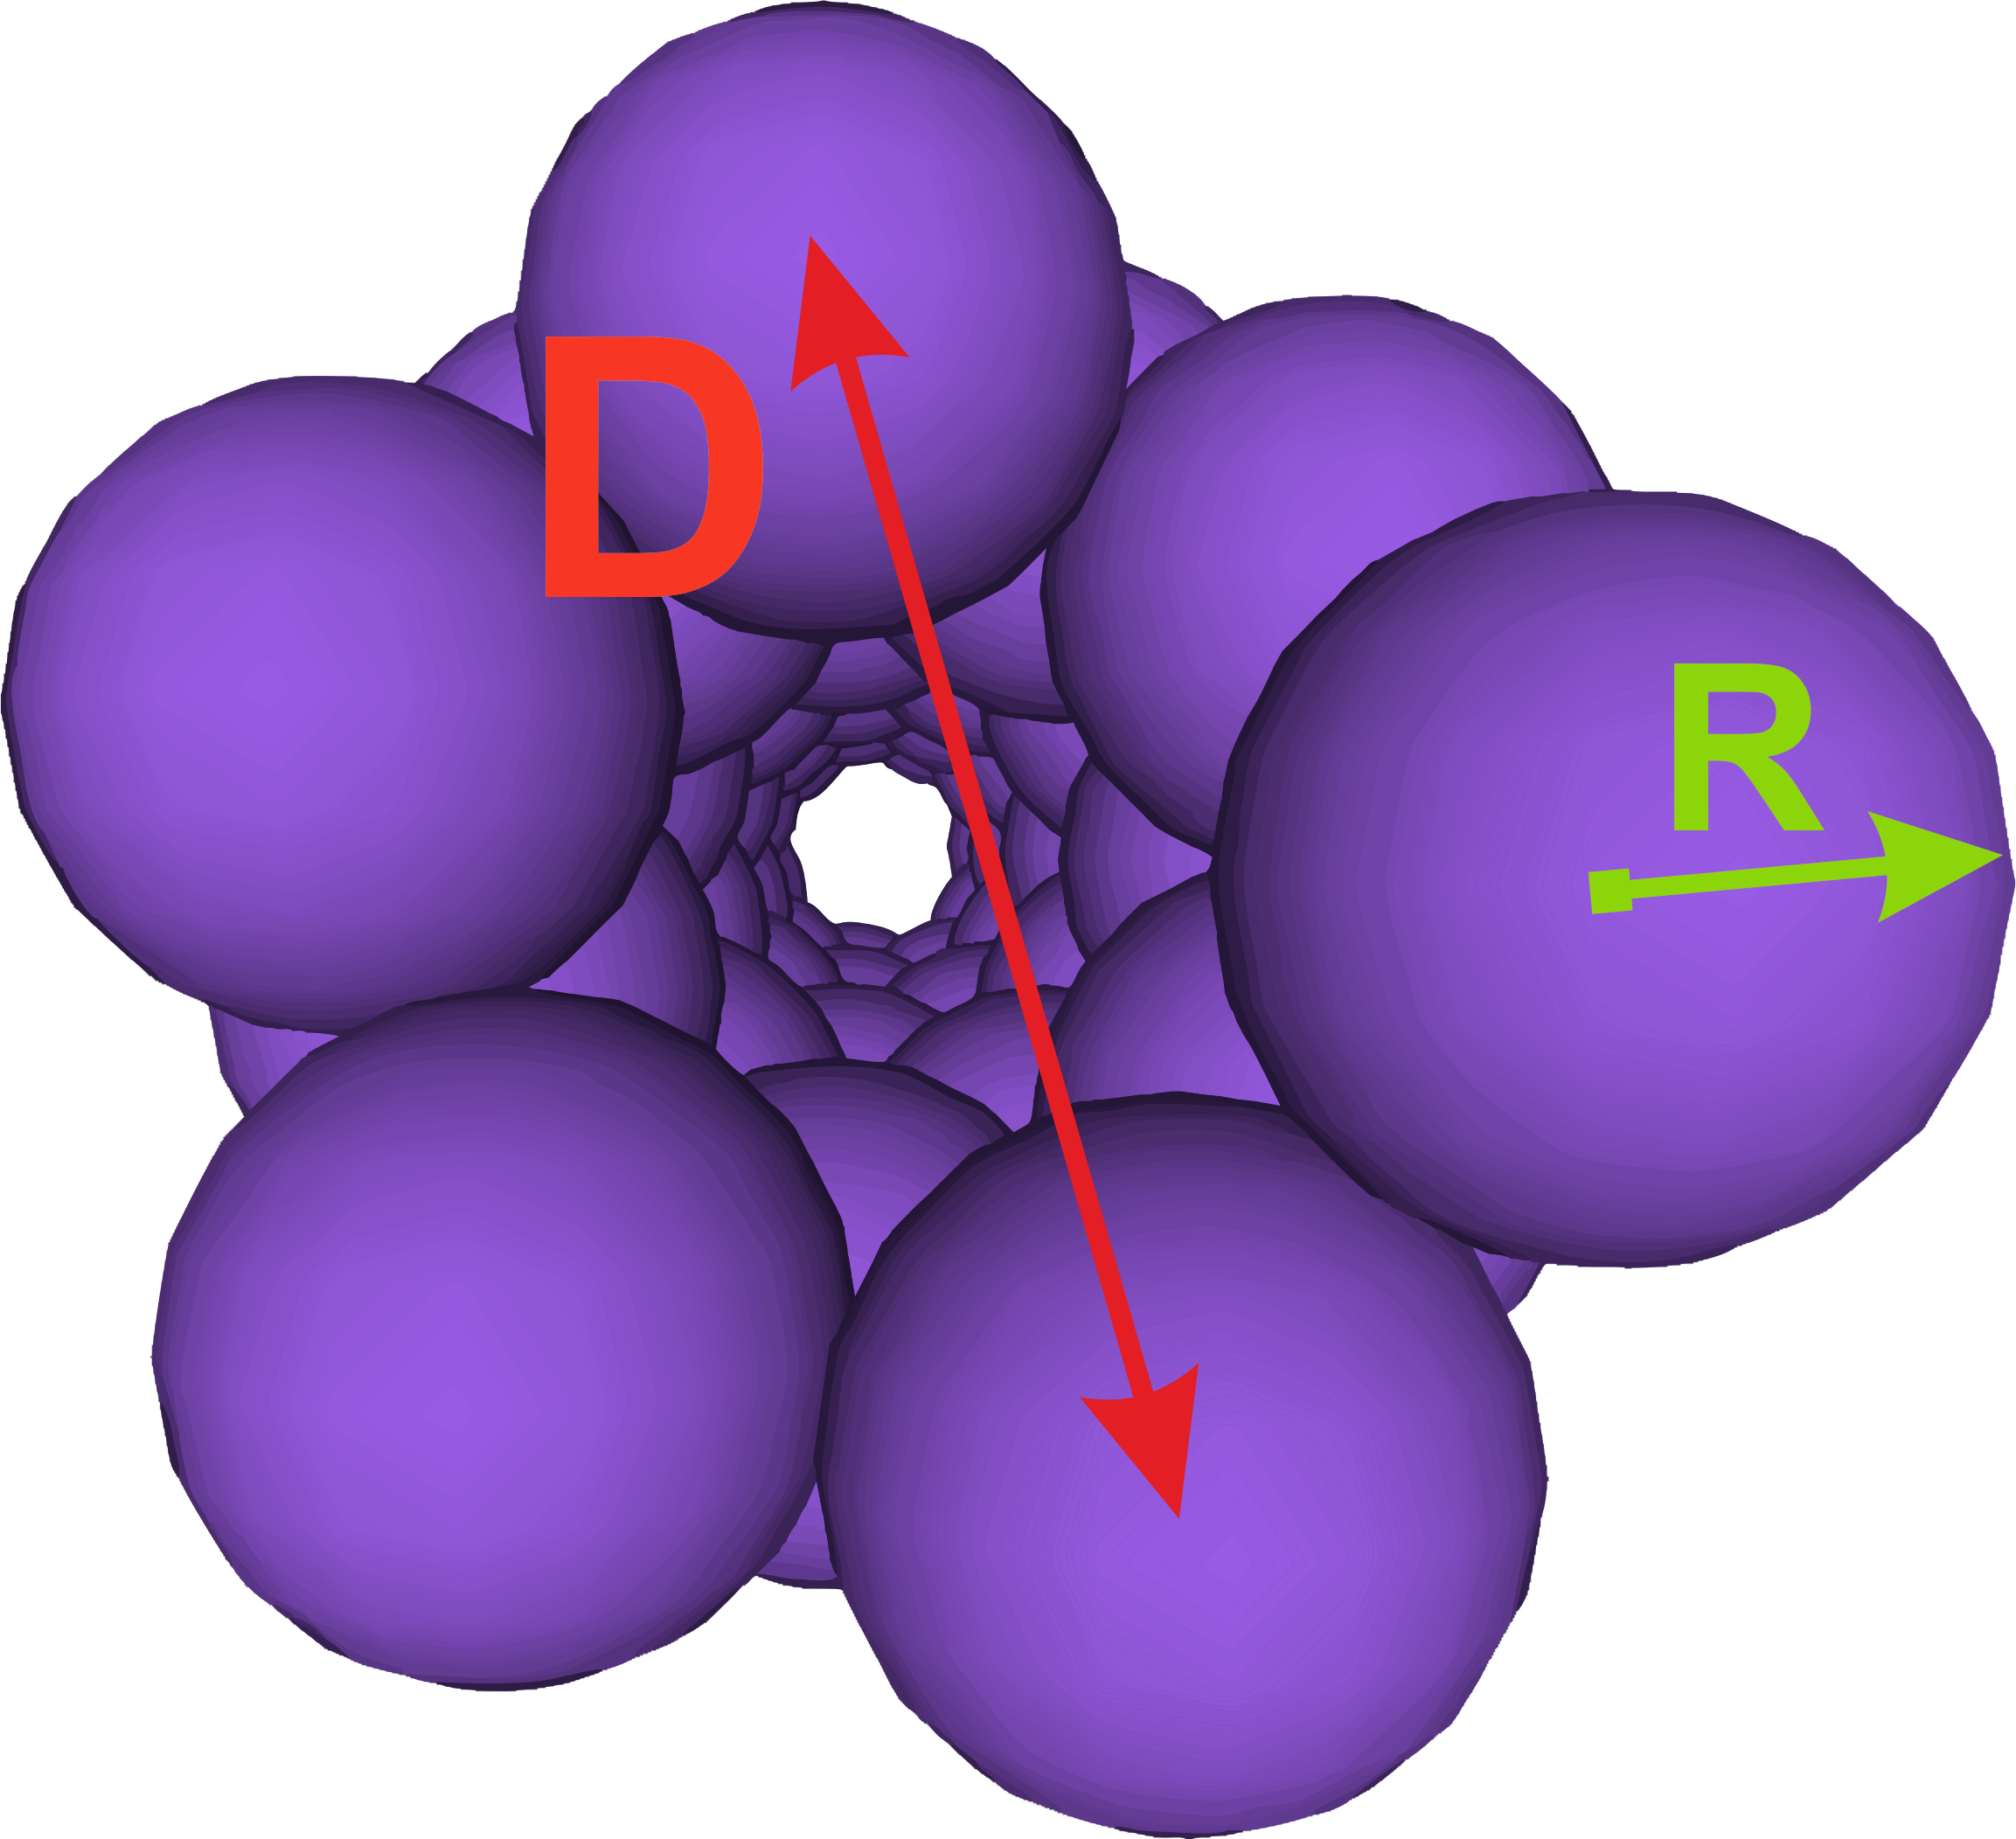
\includegraphics[width=0.9\textwidth]{../images/form_factor/cylindrical_obj/beads_helix_model_2.png}
   \caption{top on view}
   \label{fig:beadshelixside2}
\end{subfigure}
\caption{Bead model of a helix. In figure a) bead helices with different bead radius and different number of beads per turn are shown} \label{fig:beadshelix}
\end{figure}

\begin{align}
I(Q) &= P_\text{rod}(Q,H) \sum_{j=-\infty}^{\infty} \abs{\frac{nH}{P}\Psi_j\left(QD,\frac{2\pi j}{PQ}\right) \Phi(Q,R)}^2
\label{eq:beadshelix1}
\end{align}
with
\begin{align}
\Psi_j\left(QD,\frac{2\pi j}{PQ}\right) &=
\begin{cases}
\begin{array}{rcl}
J_j\left(\frac{QD}{2}\sqrt{1-\left(\frac{2\pi j}{PQ}\right)}\right) & \text{for} & Q\geq \frac{2\pi\abs{j}}{P}\\
0 & \text{for} & Q < \frac{2\pi\abs{j}}{P}
\end{array}
\end{cases}\\
\Phi(Q,R) &= 3\frac{4\pi}{3}R^3\left(\eta_\text{b}-\eta_\text{solv}\right)\frac{\sin(QR)-QR\cos{QR}}{\left(QR\right)^3} \\
P_\text{rod}(Q,H) &= H^2 \left(2\frac{\mathrm{Si}(QH)}{(QH)}-\left(\frac{\sin(QH/2)}{QH/2}\right)^2\right)
\end{align}
where $\mathrm{Si}(x)=\int_0^x\frac{\sin t}{t}\mathrm{d}t$ is the sine integral. $P_\text{rod}(Q,H)$ is the form factor of an infinitesimal thin rod of length $H$.
$J_j$ is the regular cylindrical Bessel function, for which $J_{j}(x)=(-1)^\abs{j}J_{-j}(x)$ if $j\in \mathbb{Z}$ (integer value) and $j \neq 0$.
Therefore the sum in eq.\ \ref{eq:beadshelix1} can be written as
\begin{align}
I(Q) &= P_\text{rod}(Q,H) \sum_{j=0}^{\infty} \epsilon_j \abs{\frac{nH}{P}\Psi_j\left(QD,\frac{2\pi j}{PQ}\right) \Phi(Q,R)}^2
\label{eq:beadshelix2}
\end{align}
with $\epsilon_j=1$ for $j=0$ and $\epsilon_j=2$ for $j\geq 1$.

The sum converges very fast and for small $Q$-values the first two term are already sufficient. However, {\tt SASfit} is continuing the sum until either the argument below the square root becomes negative or the relative change of the sum is less than $10^{-10}$.

The forward scattering of the model is normalized so that
\begin{align}
I(Q=0) &= \left(H\frac{nH}{P}\frac{4\pi}{3}R^3\left(\eta_\text{b}-\eta_\text{solv}\right)\right)^2
\end{align}

\vspace{5mm}

\uline{Input Parameters for model \texttt{beads helix}:}\\
\begin{description}
\item[\texttt{R}] radius of monomer units/beads $R$
\item[\texttt{D}] mean diameter of helix $D$
\item[\texttt{n}] number of monomer beads per turn $n$
\item[\texttt{dummy}] not used
\item[\texttt{dummy}] not used
\item[\texttt{P}] height of one helix period $P$
\item[\texttt{H}] total length of helix $H$
\item[\texttt{eta\_b}] scattering length density of monomer beads $\eta_\text{b}$
\item[\texttt{dummy}] not used
\item[\texttt{eta\_solv}] scattering length density of solvent $\eta_\text{solv}$
\end{description}

\noindent\uline{Note:}
\begin{itemize}
\item The helix is assumed to be stiff and long so that it scattering intensity can be factorized in a cross-section contribution and a shape contribution, whereas the shape contribution can be described by an infinitesimal thin rod of length $H$.
\item $R$, $P$, $D$, $H$, and $n$ are only physical for values larger than 0.
\item The model is an approximation for the limit $H \gg P$ and $H \gg D$.
\end{itemize}

\begin{figure}[htb]
\begin{center}
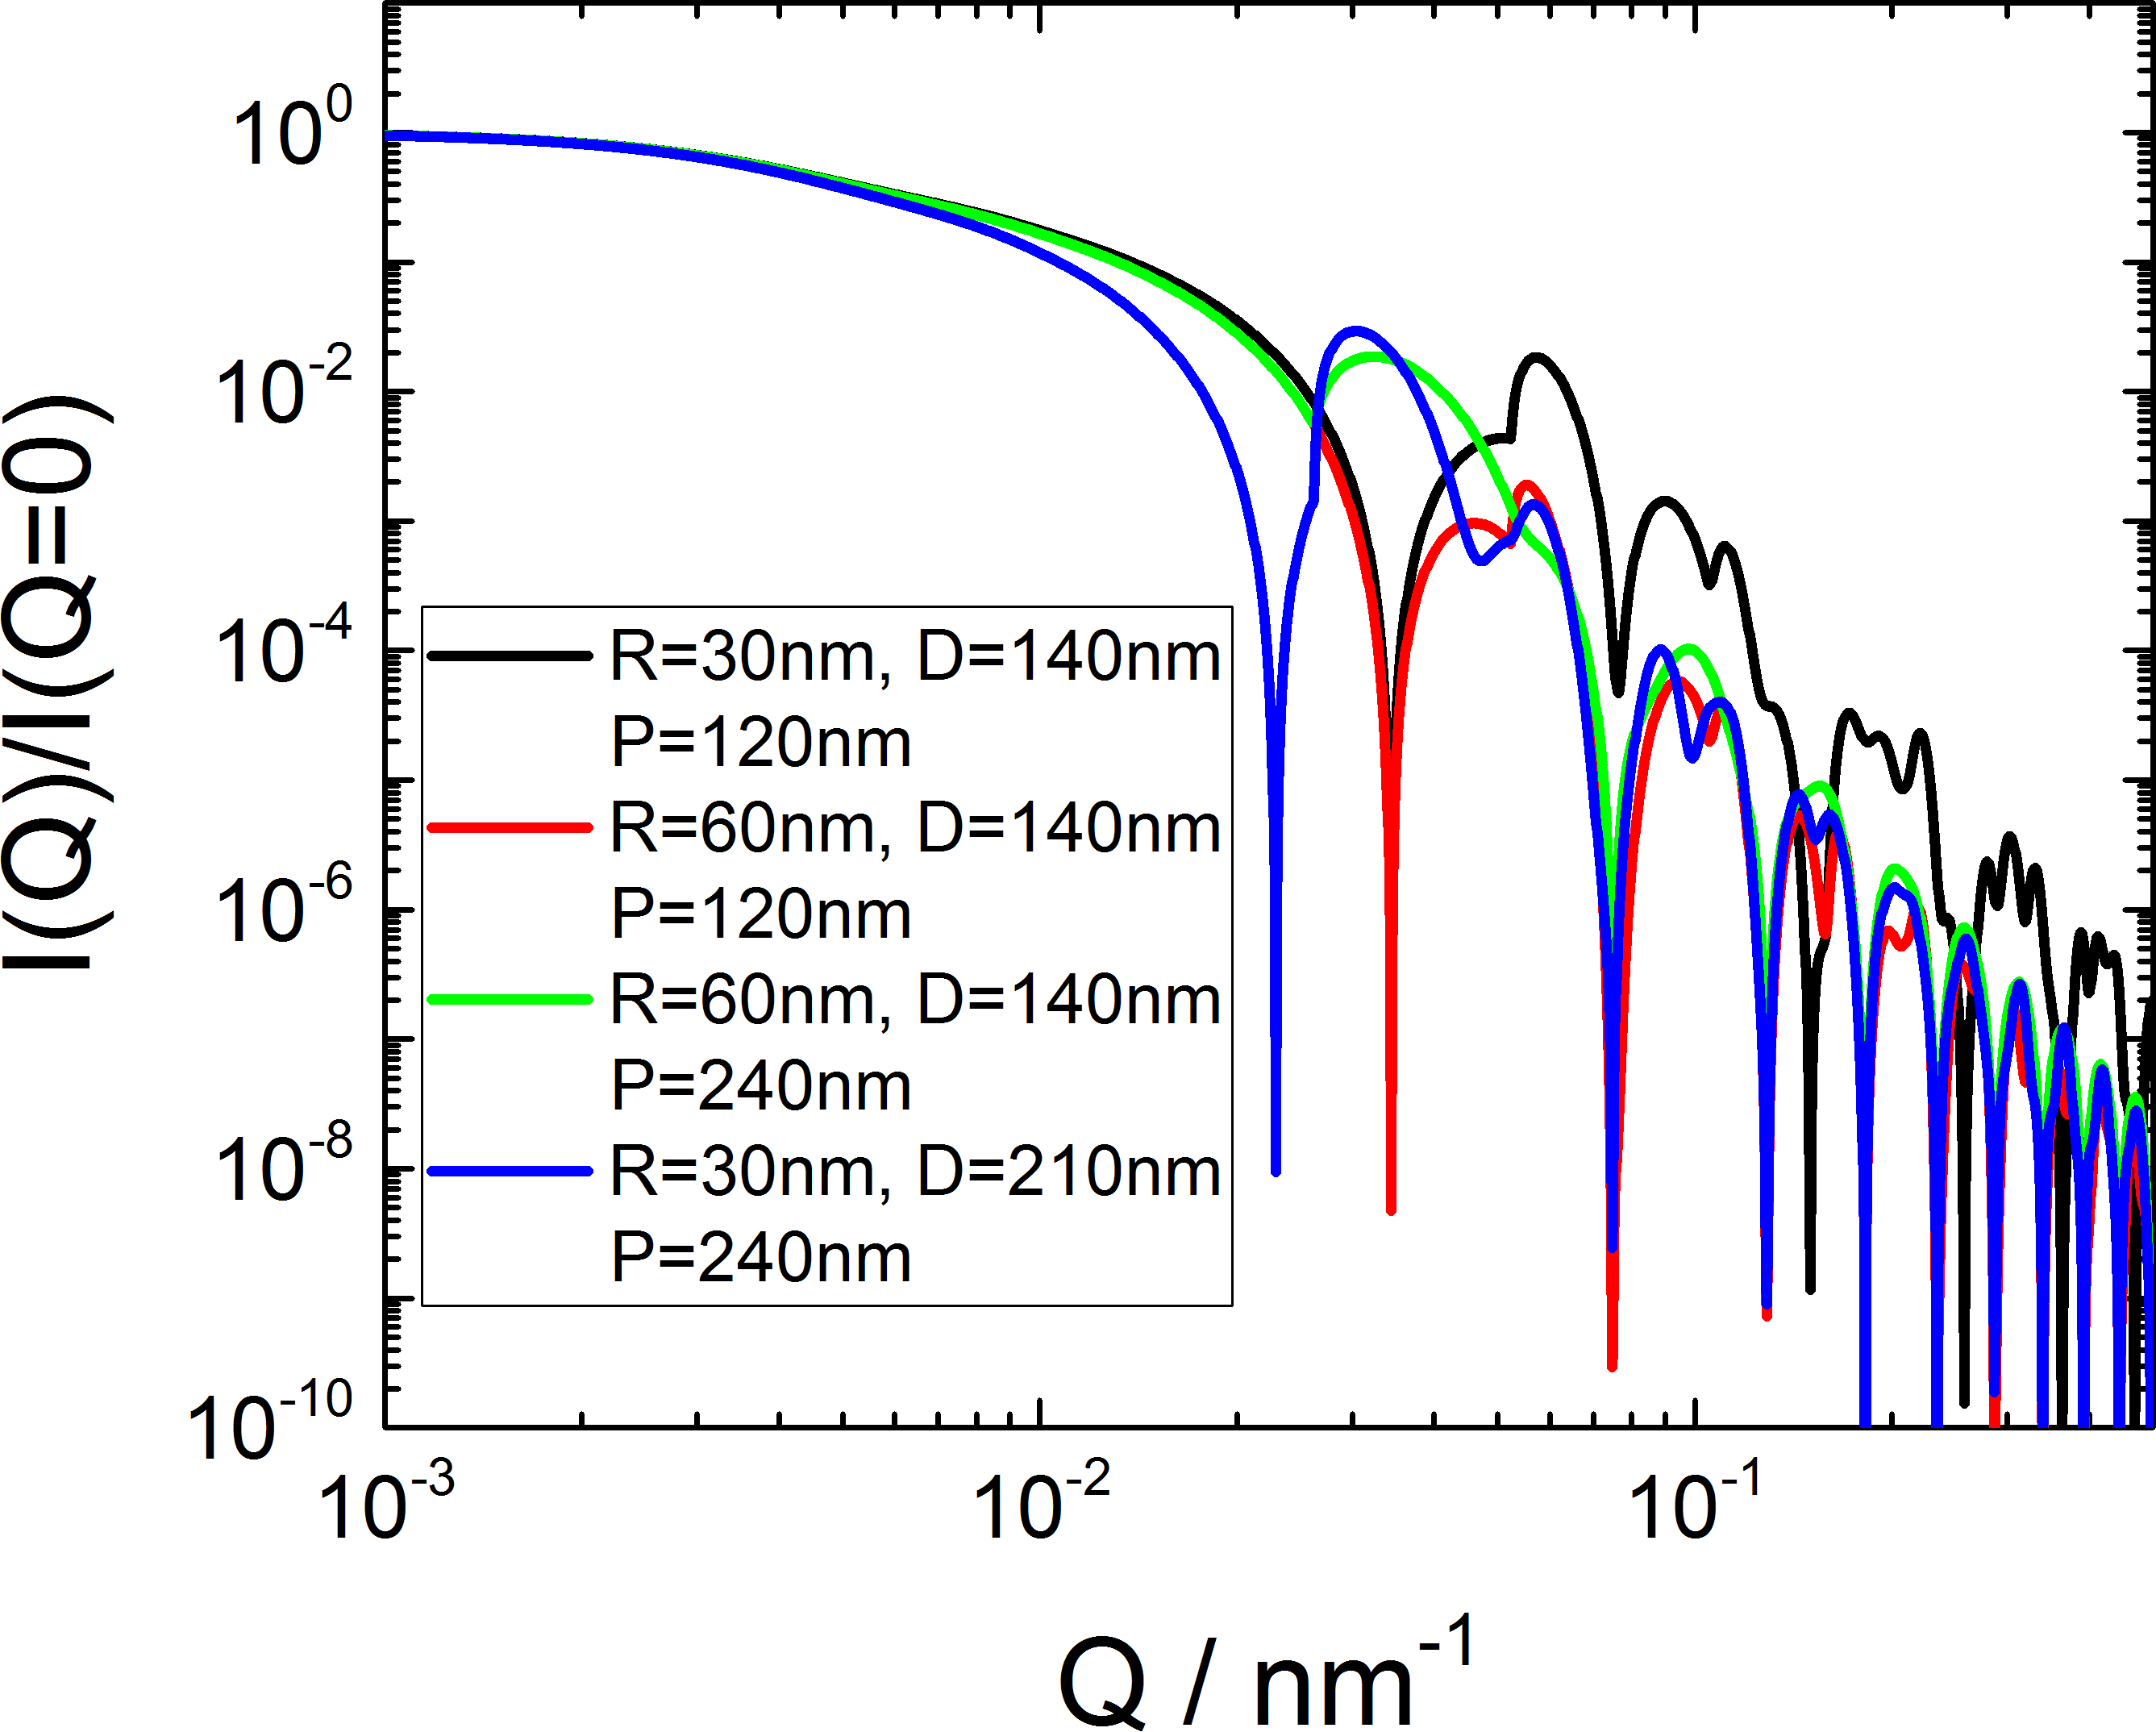
\includegraphics[width=0.7\textwidth]{../images/form_factor/cylindrical_obj/helix_beadsIQ.png}
\end{center}
\caption{Normalized scattering curves of a single stranded helices formed by spherical beads.}
\label{fig:helixbeadsIQ}
\end{figure}


%\phantom{.}~\\
\newpage
\subsubsection{straight superhelix} ~\\
Benham et al.\ \cite{Benham1980} and Crick \cite{Crick1953} describe single helices with a secondary helical curvature, which they call coiled superhelices or coiled coil. They assume in their analysis an infinitesimal thin helical strand.
\begin{figure}[htb]
\begin{center}
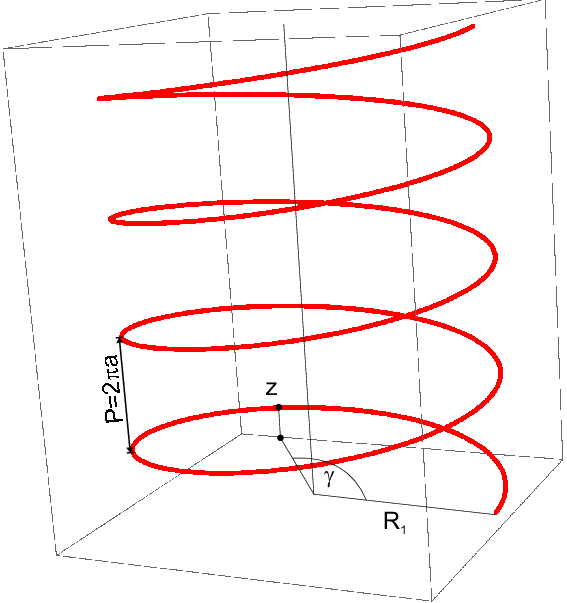
\includegraphics[width=0.497\textwidth]{../images/form_factor/cylindrical_obj/straightSuperhelix.png}
\end{center}
\caption{infinitesimal thin single stranded helix} \label{fig:straightsuperhelix}
\end{figure}
 The straight superhelix is their starting geometry without a secondary coiling. The expression for a random oriented straight superhelix of finite length can be written exact in form of a single integral and is given by
\begin{align}
I(Q) &= 2 \int_0^{\mathcal{L}} \frac{(\mathcal{L}-w)\sin Q\psi}{Q\psi} \mathrm{d}w \\
\psi &= + \sqrt{2 R_1^2\left[1-\cos\left(\frac{w}{\sqrt{R_1^2+a^2)}}\right) \right]+\frac{a^2w^2}{R_1^2+a^2}} \\
\mathcal{L} &= 2\pi \frac{H}{P} \sqrt{R_1^2+a^2} \\
a &= \frac{P}{2\pi}
\end{align}
$\mathcal{L}$ is the arclength of the helix, $R_1$ the distance to the helix axis and $P$ the pitch of the helix. The intensity is normalized to the squared arclength of the helix. i.e.
\begin{align}
I(Q=0)&=\mathcal{L}^2
\end{align}

\vspace{5mm}

\uline{Input Parameters for model \texttt{straight superhelix}:}\\
\begin{description}
\item[\texttt{R\_1}] distance to the helix axis $R_1$
\item[\texttt{dummy}] not used
\item[\texttt{dummy}] not used
\item[\texttt{dummy}] not used
\item[\texttt{dummy}] not used
\item[\texttt{P}] height of one helix period $P$
\item[\texttt{H}] total length of helix $H$
\item[\texttt{dummy}] not used
\item[\texttt{dummy}] not used
\item[\texttt{dummy}] not used
\end{description}

\noindent\uline{Note:}
\begin{itemize}
\item the model assumes an infinitesimal thin single helical strand.
\item $R_1$, $P$, and $H$ are only physical for values larger than 0.
\item The model is exact.
\end{itemize}

\begin{figure}[htb]
\begin{center}
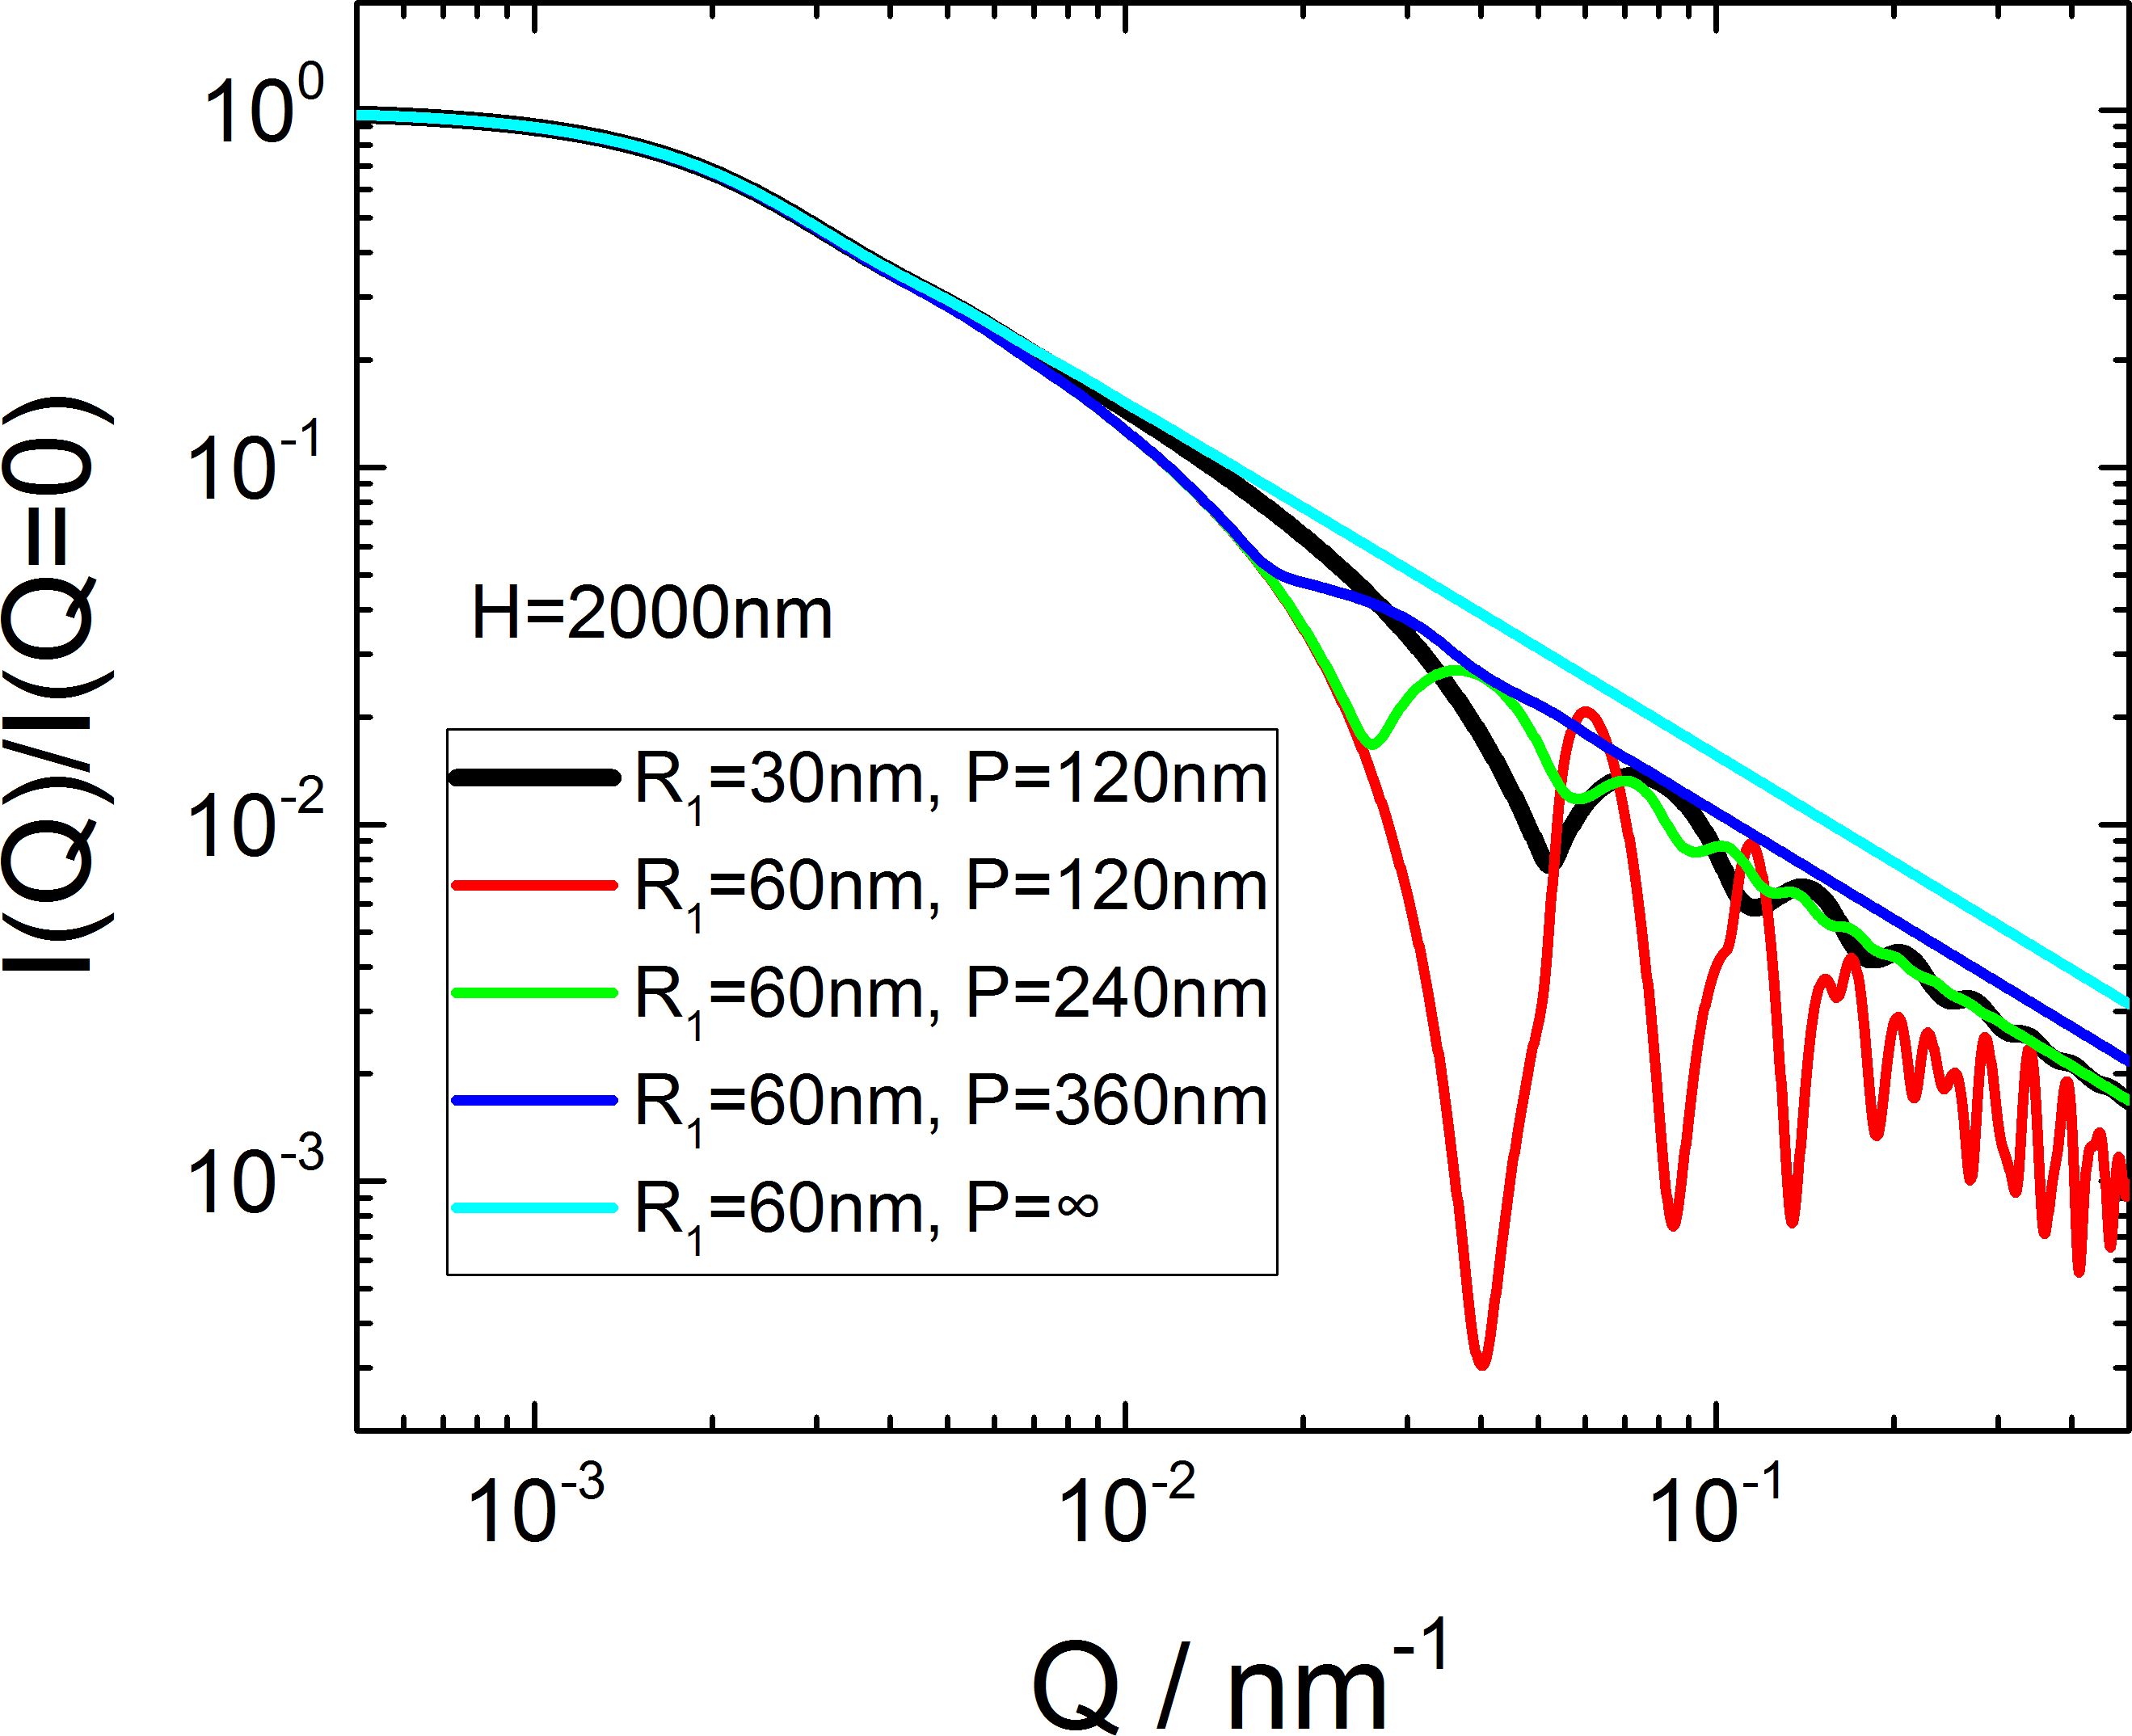
\includegraphics[width=0.7\textwidth]{../images/form_factor/cylindrical_obj/helix_straightIQ.png}
\end{center}
\caption{Normalized scattering curves of single infinitesimal thin stranded helices.}
\label{fig:helixstraightIQ}
\end{figure}

%\phantom{.}~\\
\newpage
\subsubsection{coiled superhelix} ~\\
A coiled superhelix or coiled coil is a helix with a small repeat whose axis is slightly deformed and follows a larger more graded helical path \cite{Benham1980,Crick1953}.
\begin{figure}[htb]
\captionsetup[subfigure]{position=b}
\centering
\subcaptionbox{[A superhelix with primary and secondary turns. The bottom one has ten times more primary turns per secondary turn than the top one \label{fig:superhelixcoiled1} }{
\begin{minipage}[b]{0.45\textwidth}
  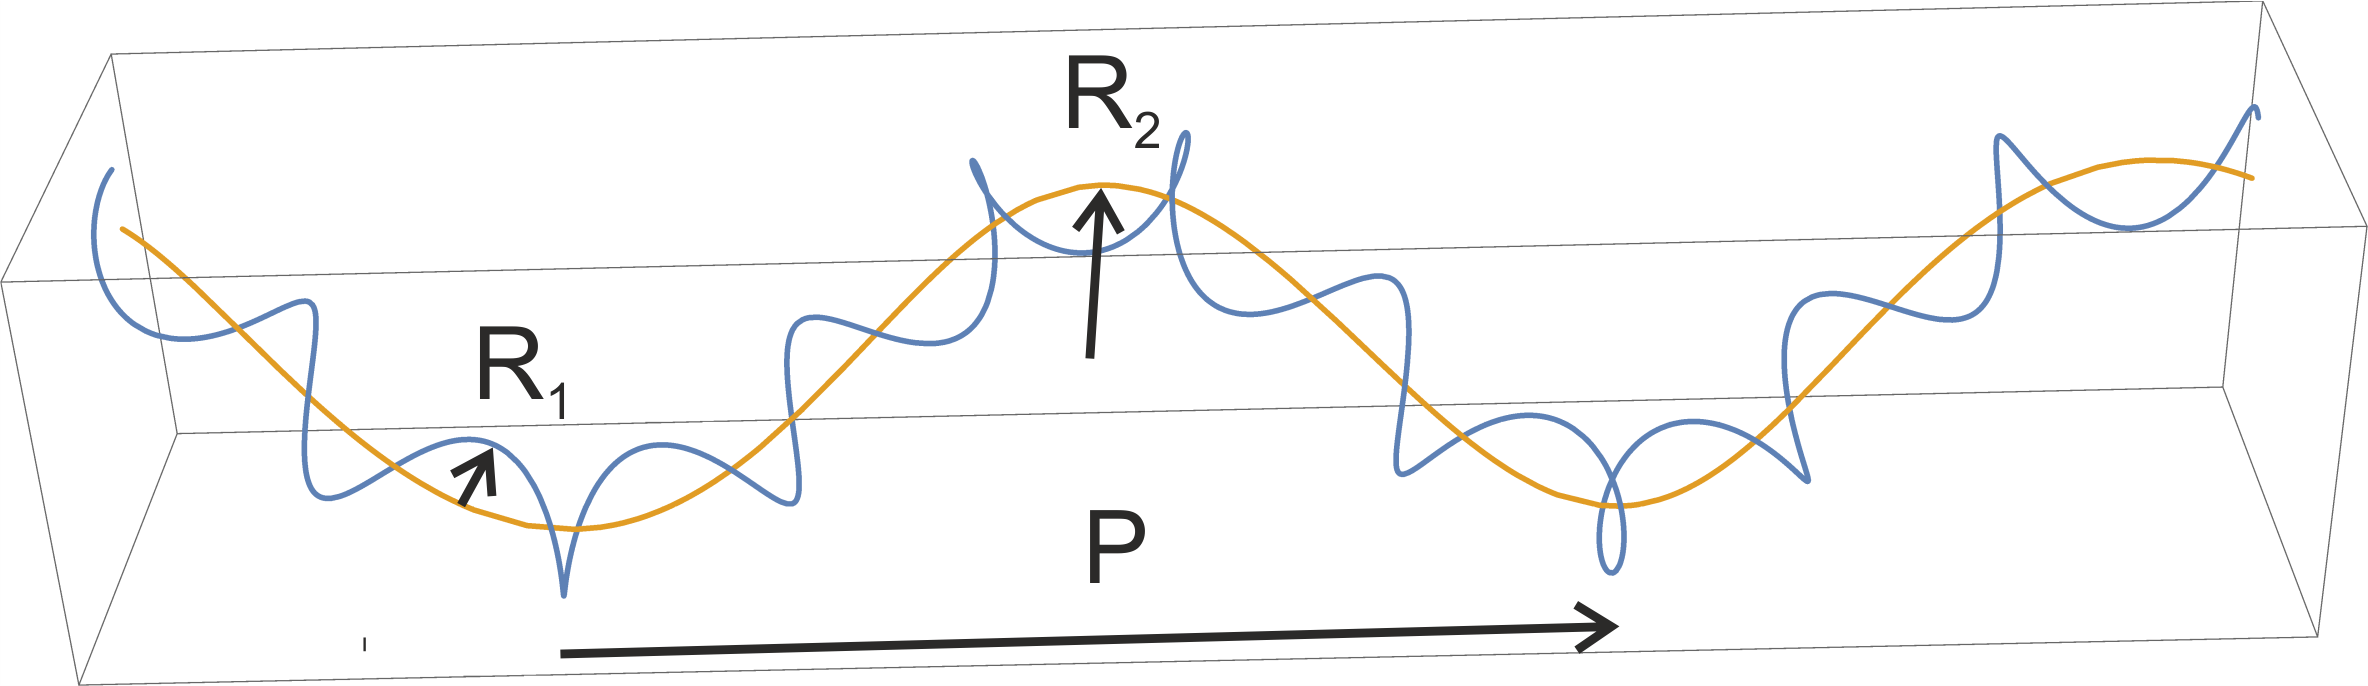
\includegraphics[width=\textwidth]{../images/form_factor/cylindrical_obj/superhelixcoiled1.png} \\
  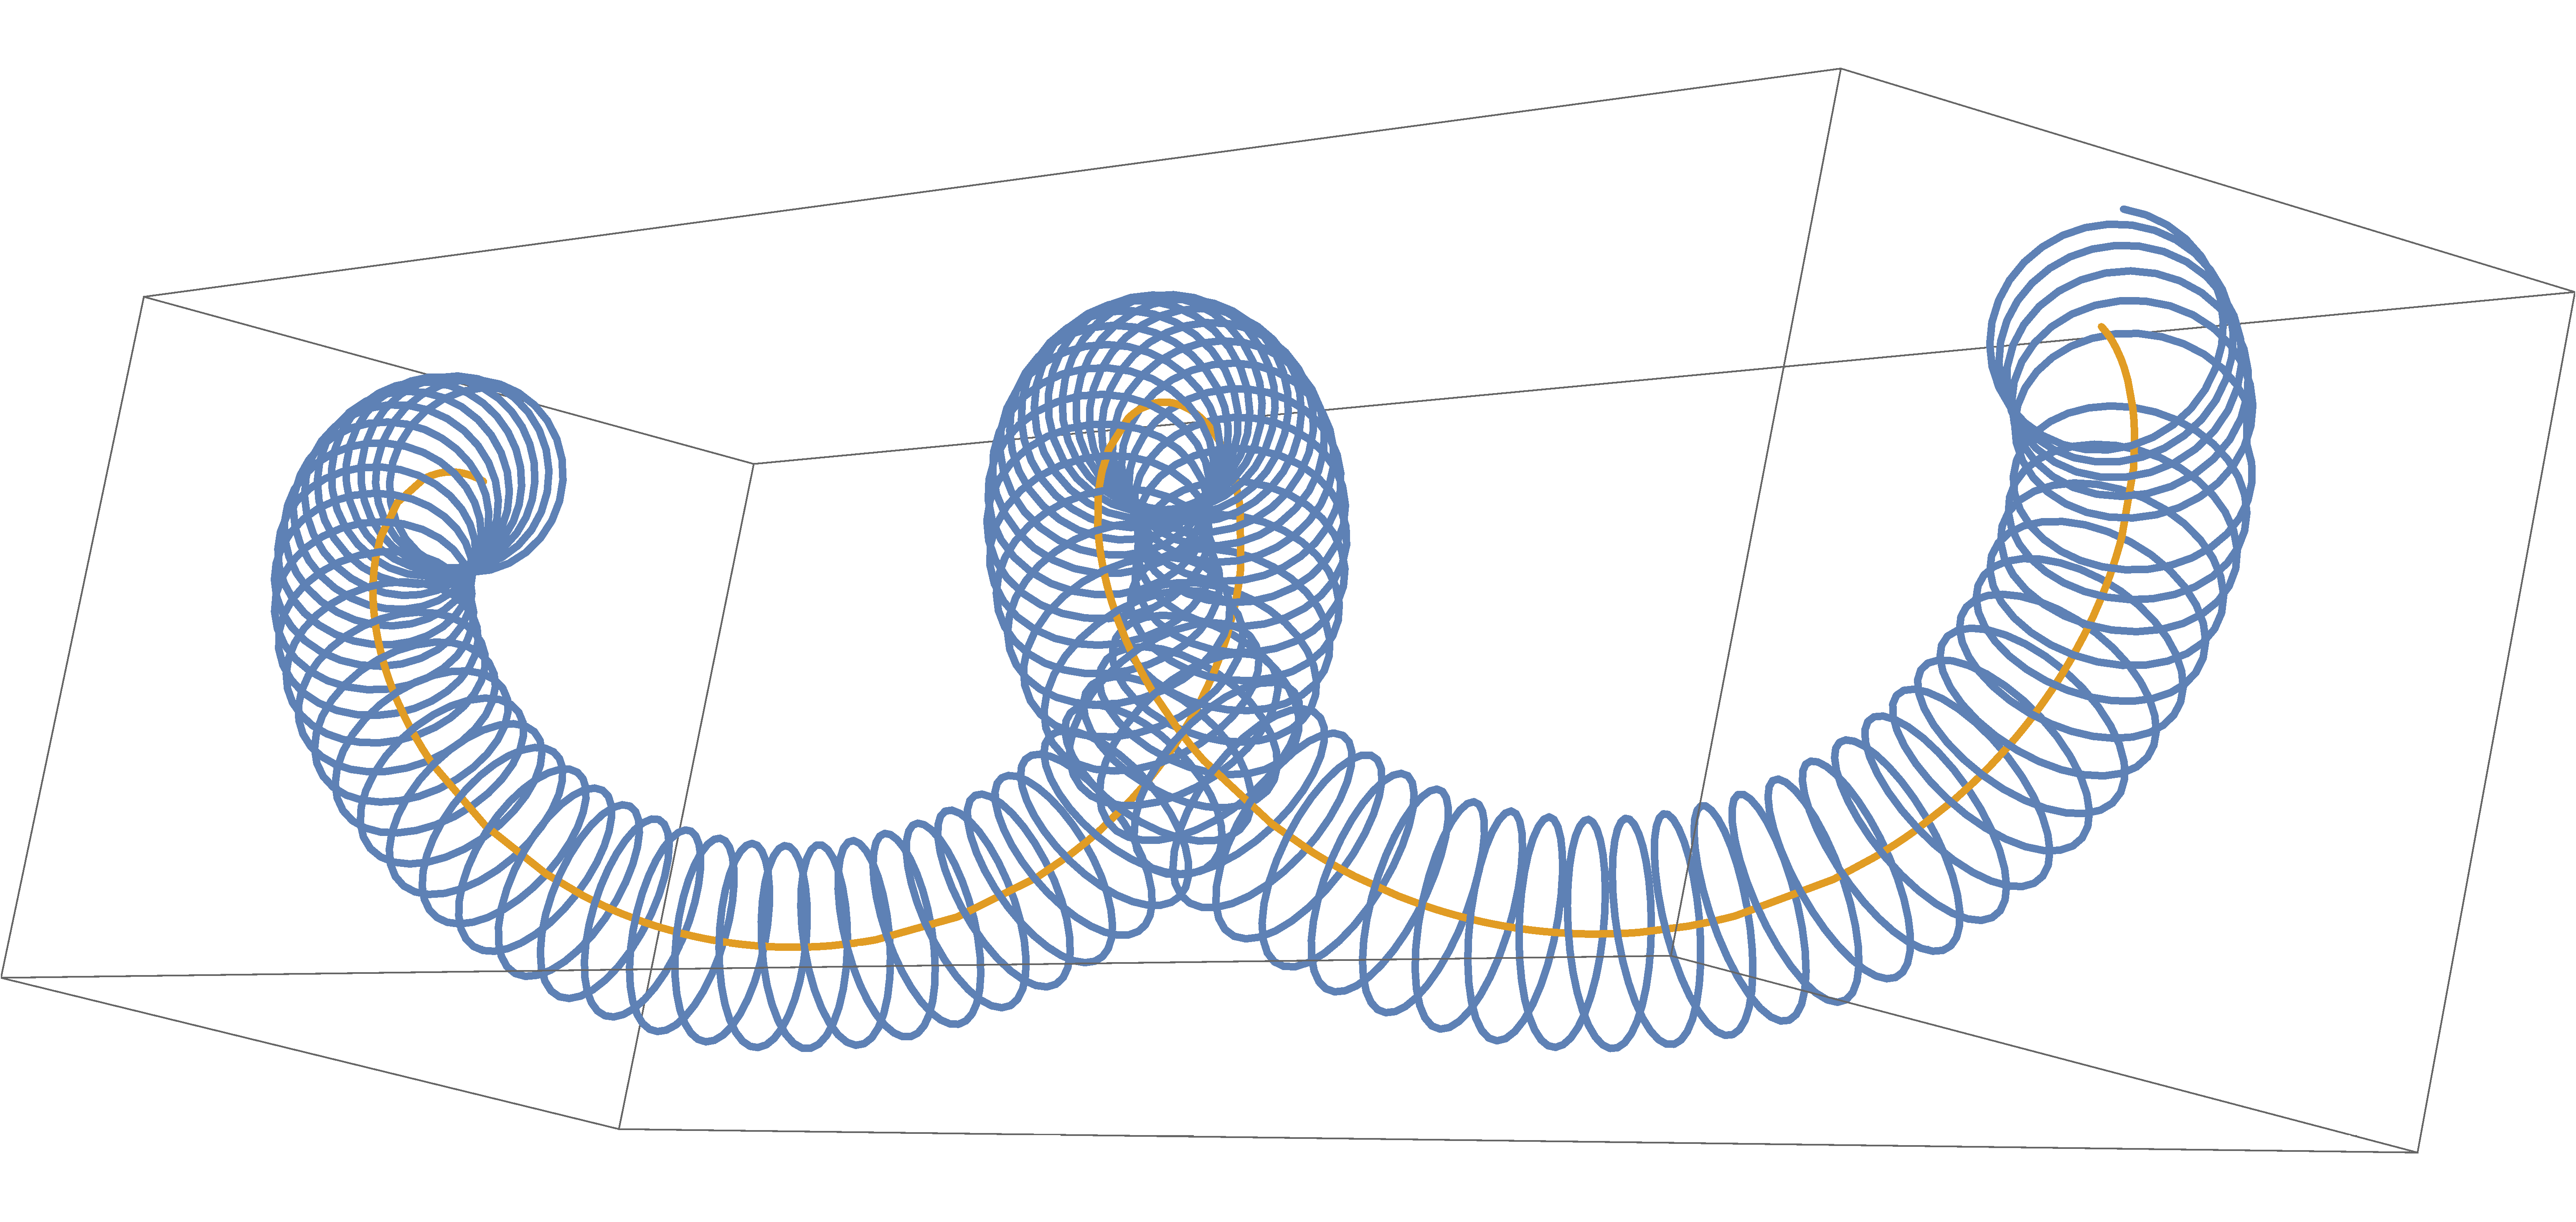
\includegraphics[width=\textwidth]{../images/form_factor/cylindrical_obj/superhelixcoiled2.png}
  \end{minipage}
}
\hfill
\subcaptionbox{A superhelix with zero pitch forms a toroidal helix \label{fig:superhelixcoiled2} }{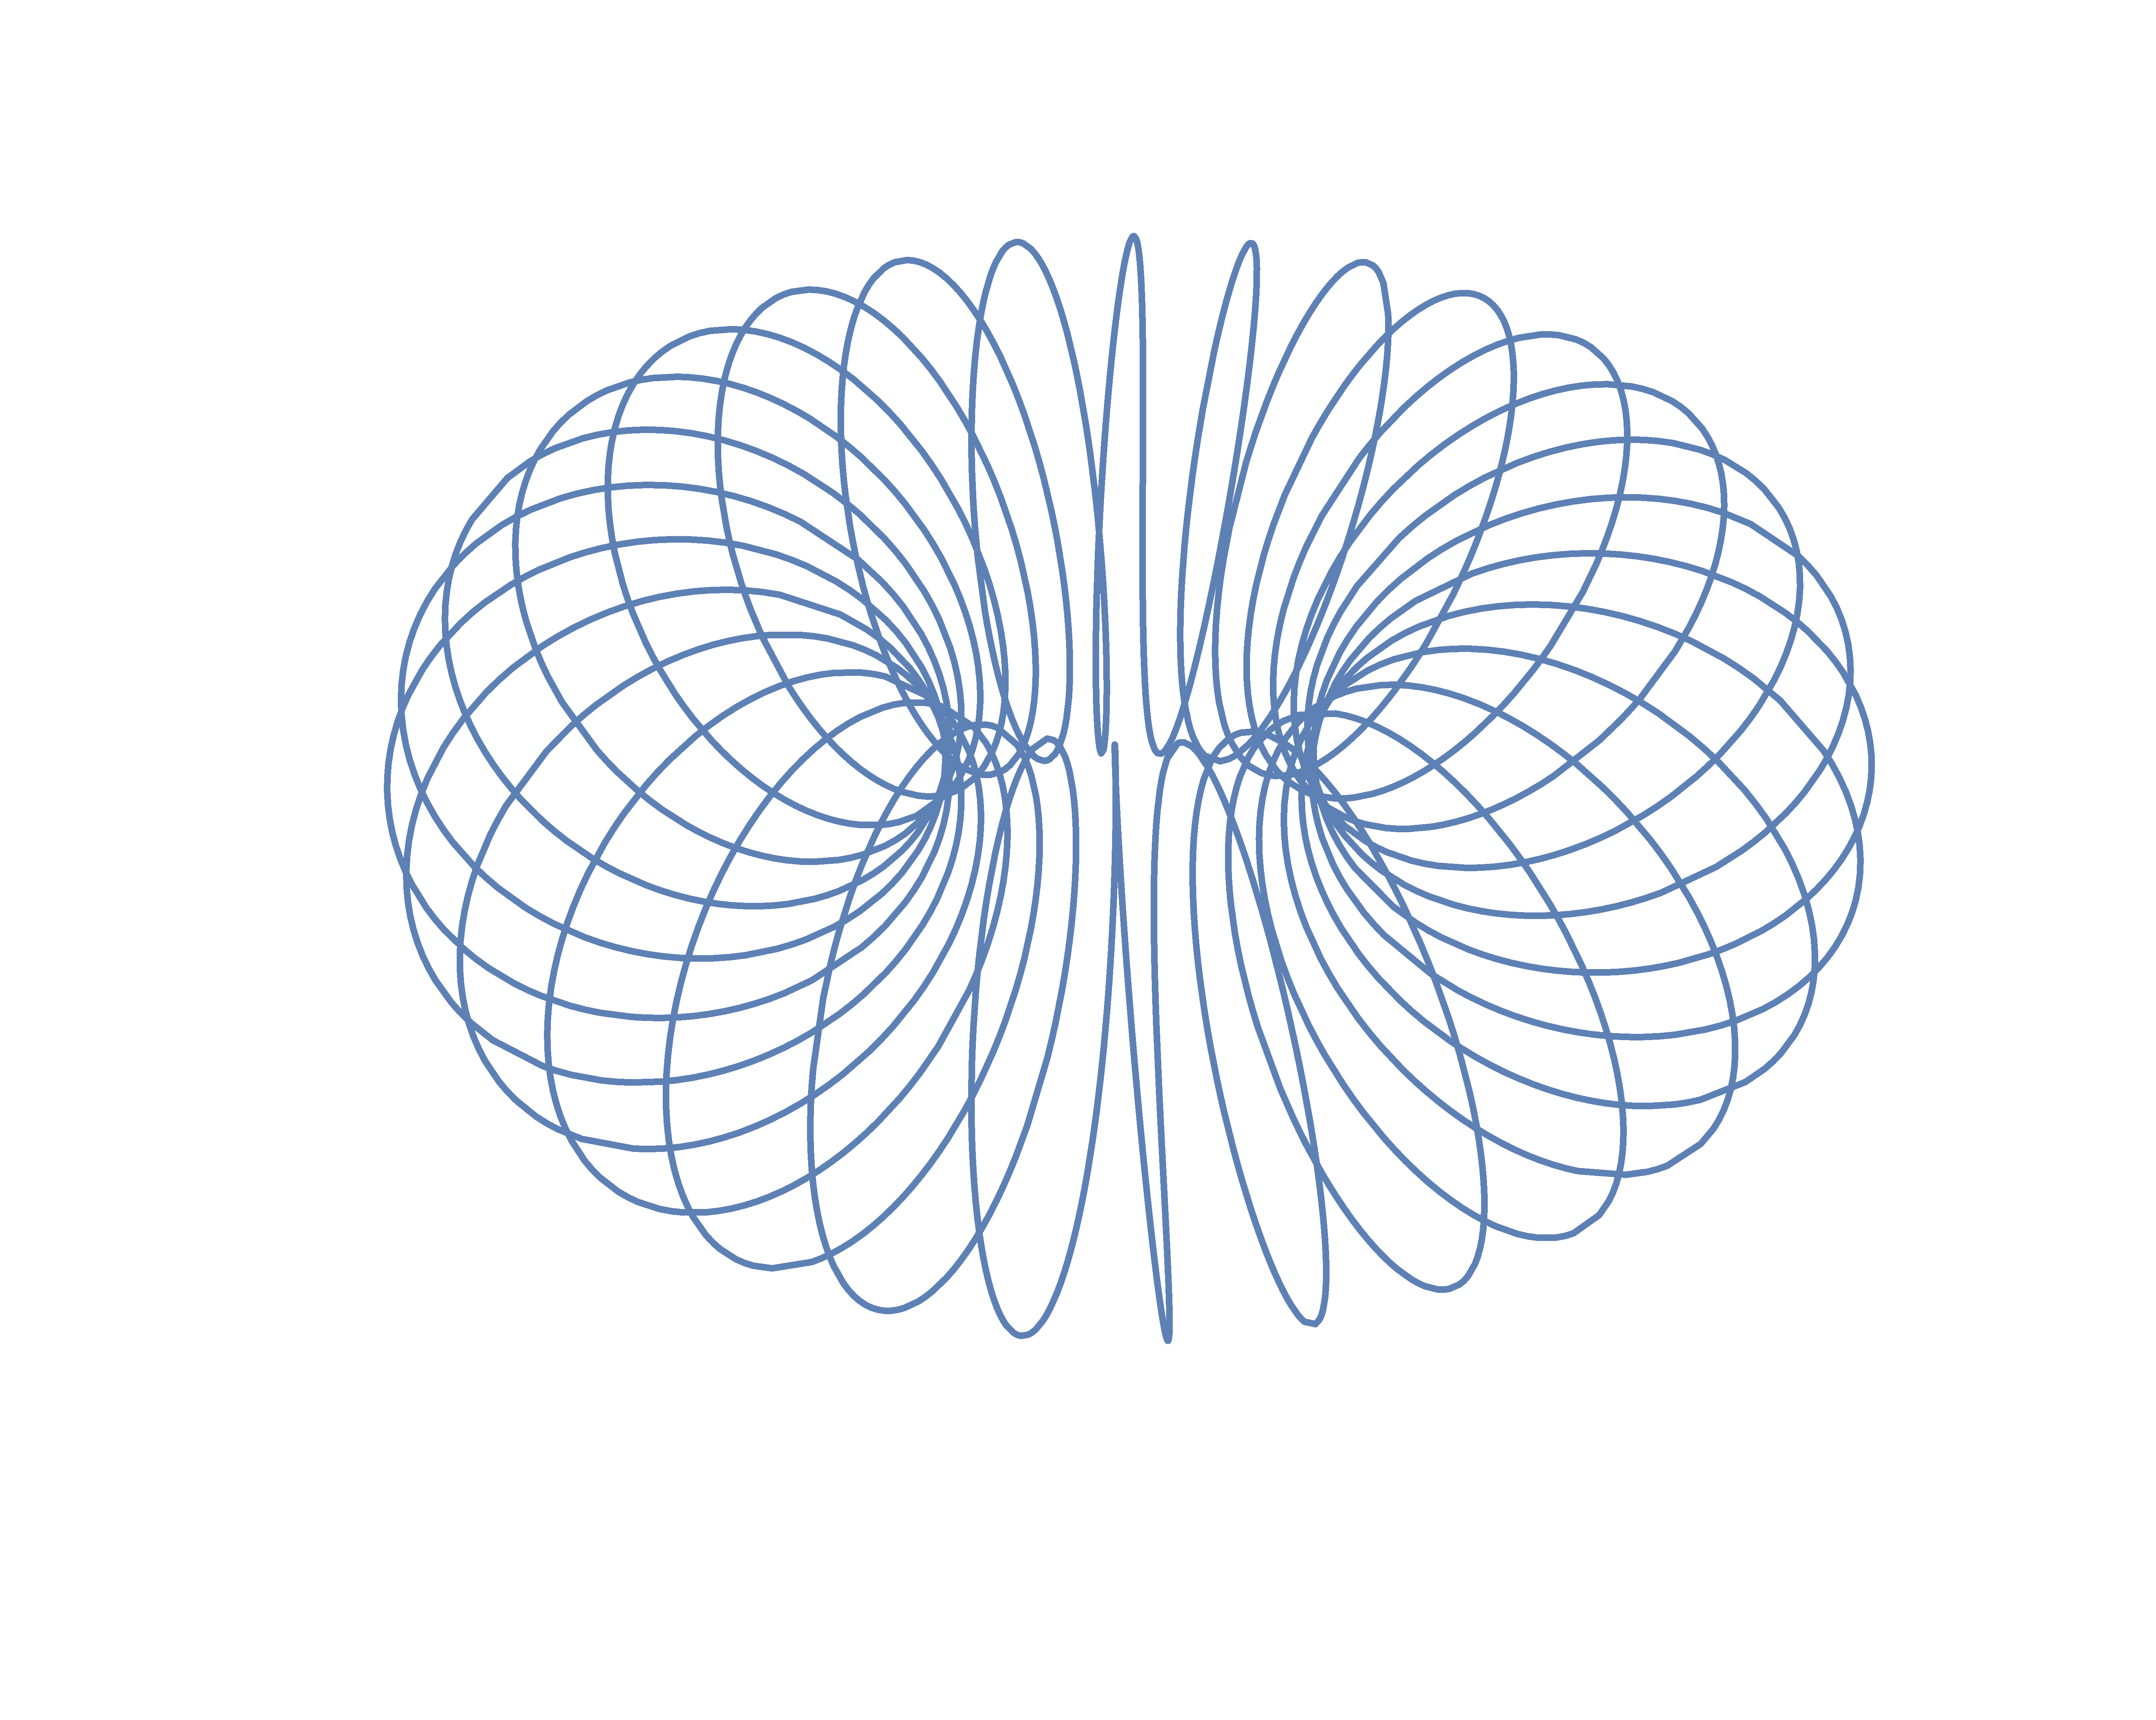
\includegraphics[width=0.45\textwidth]{../images/form_factor/cylindrical_obj/superhelixcoiled3.png}}
\caption{Combinations of two helical orders are
referred to as coiled coils or coiled superhelix.} \label{fig:superhelixcoiled}
\end{figure}


The points $p(\gamma)=\left[x(\gamma),y(\gamma),z(\gamma)\right]$ on the coiled superhelix are parametrized by
\begin{align}
x(\gamma) &= \cos\left(\gamma\right) \left(R_2+R_1\cos\left(N\gamma\right)\right)
            - R_1\cos\left(\alpha_2\right)\sin\left(\gamma\right)\sin\left(N\gamma\right) \\
y(\gamma) &= \sin\left(\gamma\right) \left(R_2+R_1\cos\left(N\gamma\right)\right)
            - R_1\cos\left(\gamma\right)\sin\left(N\gamma\right)\cos\left(\alpha_2\right) \\
z(\gamma) &= \frac{P}{2\pi}\gamma - R_1\sin\left(\alpha_2\right)\sin\left(N\gamma\right)
\end{align}
$R_1$ and $R_2$ are the radii of the primary and secondary coiling of the superhelix. $P$ is the pitch of the secondary coiling and $\alpha_2= \arctan\left(\frac{2\pi R_2}{P}\right)$ its pitch angle. $N$ is the number of first order tuns in the primary coiling for each turn of the secondary coiling.
The arc length of the helix $\mathcal{L}$ can be calculated by
\begin{align}
\mathcal{L} &= \int_0^{\gamma_\mathrm{max}} \sqrt{f(\gamma)} \mathrm{d}\gamma
\end{align}
with
\begin{align}
\begin{split}
f(\gamma) &= R_2^2+R_1^2N^2 \left(\cos^2\left(N\gamma\right)+\sin^2\left(N\gamma\right)\cos^2(\alpha_2)\right) \\
&+\frac{P^2}{(2\pi)^2} + 2R_2R_1\cos\left(N\gamma\right) +2R_1^2N\cos(\alpha_2)
\end{split}
\end{align}
and
\begin{align}
\gamma_\mathrm{max} &= 2\pi N_\mathrm{2nd}
\end{align}
where $N_\mathrm{2nd}$ is the number of secondary turns of the coiled superhelix.
The scattering intensity is than given by
\begin{align}
I(Q) &= \int_0^{\gamma_\mathrm{max}} \mathrm{d}\gamma_2 \int_0^{\gamma_\mathrm{max}} \sqrt{f(\gamma_2)f(\gamma_1)}
\frac{\sin\left( Qr(\gamma_1,\gamma_2)\right)}{Qr(\gamma_1,\gamma_2)} \mathrm{d}\gamma_2
\end{align}
with
\begin{align}
r^2(\gamma_1,\gamma_2) &= \left( \begin{pmatrix}
                            x(\gamma_2) \\
                            y(\gamma_2) \\
                            z(\gamma_2) \\
                          \end{pmatrix}
                        - \begin{pmatrix}
                            x(\gamma_1) \\
                            y(\gamma_1) \\
                            z(\gamma_1) \\
                          \end{pmatrix} \right)^2
\end{align}
The intensity is normalized to the squared arclength of the helix. i.e.
\begin{align}
I(Q=0)&=\mathcal{L}^2
\end{align}

\vspace{5mm}

\uline{Input Parameters for model \texttt{coiled superhelix}:}\\
\begin{description}
\item[\texttt{R\_1}] distance to the primary helix axis $R_1$
\item[\texttt{R\_2}] distance to the primary helix axis $R_1$
\item[\texttt{dummy}] not used
\item[\texttt{N}] number of primary turns $N$ per secondary turn
\item[\texttt{dummy}] not used
\item[\texttt{P}] pitch length of secondary helix $P$
\item[\texttt{turns}] number of secondary turns $N_\mathrm{2nd}$
\item[\texttt{dummy}] not used
\item[\texttt{dummy}] not used
\item[\texttt{dummy}] not used
\end{description}

\noindent\uline{Note:}
\begin{itemize}
\item the model assumes an infinitesimal thin single helical strand with an additional secondary coiling.
\item $R_1$,$R_2$, $P$, $N_\mathrm{2nd}$ and $N$ are only physical for values larger than 0.
\item The model is exact.
\item The calculation of the scattering intensity requires a double integration, which is the reason for the longer computing time.
\end{itemize}

\begin{figure}[htb]
\begin{center}
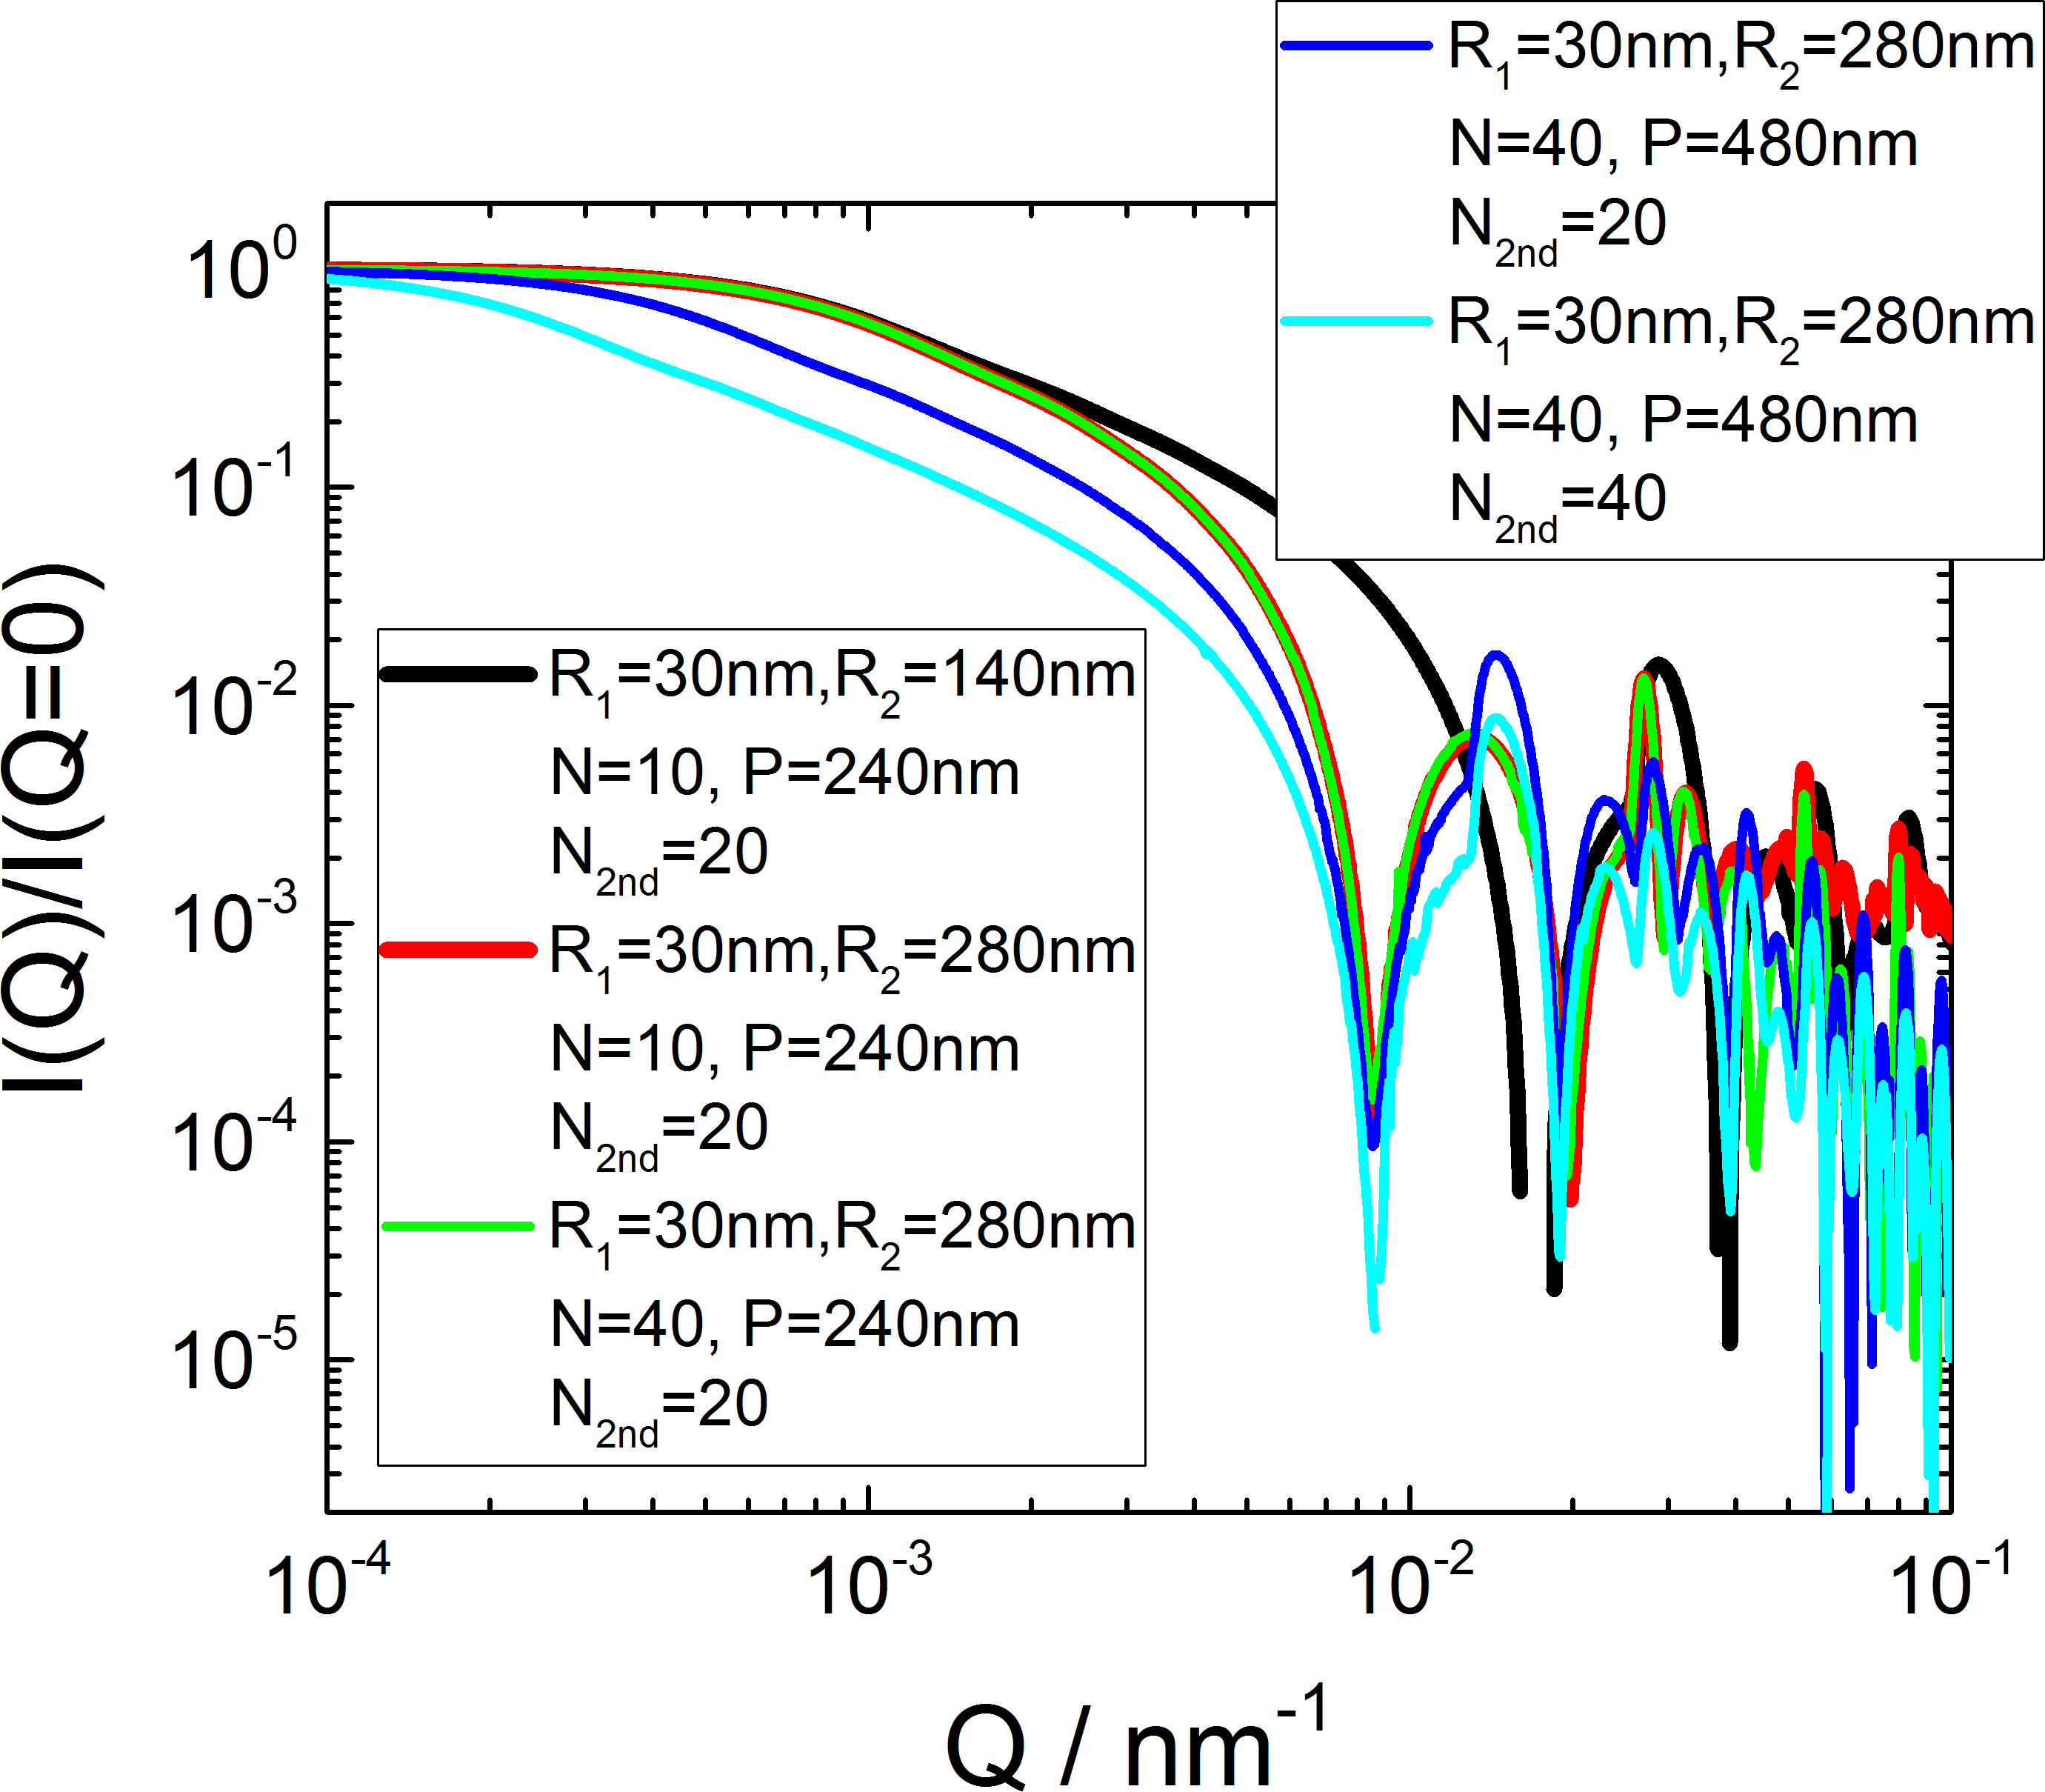
\includegraphics[width=0.7\textwidth]{../images/form_factor/cylindrical_obj/helix_coiledIQ.png}
\end{center}
\caption{Normalized scattering curves of single stranded infinitesimal thin coiled helices.}
\label{fig:helixcoiledIQ}
\end{figure} 